% Class, Font size, Paper shape, isDraft
\documentclass[a4paper, 10pt, final]{article} % Document class: [draft] sets pdf output to draft quality, [<number>pt] sets font size in range of 10-12pt
\usepackage{import} % Import other latex documents (here for 3d plot variables definition)
\usepackage{shellesc}

%% Todo
\usepackage[obeyFinal]{easy-todo}

%% Margins
\usepackage[margin=2.5cm]{geometry} % Margins: \newgeometry{<options>} can set margins individually

%% Language, Fonts, Encoding
\usepackage[english]{babel}                         % Input encoding language
\usepackage{fontspec}                               % XeTeX font settings
\defaultfontfeatures{Ligatures=TeX, Numbers=Lining} % OTF font features for all fonts
\setmainfont{Linux Libertine O}                     % Set serif (main) font
\setsansfont{Linux Biolinum O}                      % Set sans serif font
\setmonofont{Inconsolata}                           % Set monospace font
\usepackage{amsmath, amssymb}                       % Math support
\newcommand{\mathbff}[1]{$\boldsymbol{#1}$}

%% Paragraph, Line spacings
\setlength{\parindent}{2em}
\setlength{\parskip}{1.5ex}
\renewcommand{\baselinestretch}{1.0}

%% Text alignment
\usepackage{ragged2e} % Text alignment correction (\Centering, \RaggedRight, \RaggedLeft, \justifying)

%% Headers & Footers
\usepackage{fancyhdr}                                                        % Headers conFiguration package
\pagestyle{fancy}                                                            % {fancy}: keyword for custom headers and footers
\fancyhead[L]{\textbf{LAM: Design of Analog Filters}}                           % Header settings
\fancyhead[R]{2021/2022}
\fancyfoot[R,L]{}                                                            % Footer settings
\fancyfoot[C]{\thepage}
\renewcommand{\headrulewidth}{0.5pt}                                         % Header line thickness
\renewcommand{\footrulewidth}{1pt}                                           % Footer line thickness
\usepackage[stable, marginal, bottom, para]{footmisc}                        % Footers fix: [stable] prevents footers in titles, [bottom] deletes space left on the bottom,[marginal] puts footers near margin, [para] puts multiple footers on one line
\renewcommand{\footnoterule}{\noindent\smash{\rule[3pt]{\textwidth}{0.5pt}}} % Footnote line

%% Bibliography, References
\usepackage[style=apa, sorting=nty]{biblatex}             % Bibliography: [style=apa] won't mix references with footer naming, [sorting=nty] "Name, Title, Year" is most sensible to use in terms of searchability
\usepackage{csquotes}                                     % Babel & quotes behaviour fix
\addbibresource{LAM_Design_dei_filtri_analogici.bib}      % File with bibliograpy sorces information
\newcommand{\parenciteit}[2]{\textit{\parencite[#1]{#2}}} % Italic parencite (citation in parenthesis)
\usepackage{hyperref}                                     % Clickable references: [hidelinks]
\hypersetup{
    colorlinks=true,
    linkcolor=blue,
    filecolor=blue,
    citecolor=blue,
    urlcolor=cyan,
}
%% Biblates Hyperref fix
\DeclareFieldFormat{citehyperref}{%
  \DeclareFieldAlias{bibhyperref}{noformat}% Avoid nested links
  \bibhyperref{#1}}

\DeclareFieldFormat{textcitehyperref}{%
  \DeclareFieldAlias{bibhyperref}{noformat}% Avoid nested links
  \bibhyperref{%
    #1%
    \ifbool{cbx:parens}
      {\bibcloseparen\global\boolfalse{cbx:parens}}
      {}}}

\savebibmacro{cite}
\savebibmacro{textcite}

\renewbibmacro*{cite}{%
  \printtext[citehyperref]{%
    \restorebibmacro{cite}%
    \usebibmacro{cite}}}

\renewbibmacro*{textcite}{%
  \ifboolexpr{
    ( not test {\iffieldundef{prenote}} and
      test {\ifnumequal{\value{citecount}}{1}} )
    or
    ( not test {\iffieldundef{postnote}} and
      test {\ifnumequal{\value{citecount}}{\value{citetotal}}} )
  }
    {\DeclareFieldAlias{textcitehyperref}{noformat}}
    {}%
  \printtext[textcitehyperref]{%
    \restorebibmacro{textcite}%
    \usebibmacro{textcite}}}

%% Graphics
\usepackage{graphicx}                                    % Support for images
\usepackage{ifluatex}
% \ifluatex
%   \usepackage{pdftexcmds}
%   \makeatletter
%   \let\pdfstrcmp\pdf@strcmp
%   \let\pdffilemoddate\pdf@filemoddate
%   \makeatother
% \fi
\usepackage{pdfpages}                             % Support for pdf insertion
\usepackage{tikz}                                        % Support for vector graphics
\usetikzlibrary{
    calc,                                                % Support for coordinate operations in tikz
    patterns,                                            %
    positioning,                                         %
    shapes.geometric,                                    %
    shapes.arrows,                                       %
    decorations.pathmorphing,                            %
    matrix,                                              %
    chains,                                              %
    scopes,                                              %
    arrows,                                              %
    fit,                                                 %
    shadows,                                             %
    backgrounds                                          %
}
% \usepackage{pgfkeys}
\usepackage{float}                                       % Support for floats fix
\usepackage[section]{placeins}                           % Support for FloatBarrier
\usepackage{caption}                                     % Support for cpations inside tikz
\usepackage{subcaption}                                  % Support for captions inside subfigures
\usepackage[nooldvoltagedirection, european]{circuitikz} % Support for electric circuit diagrams
\def \circuitsscale{0.6}                                 % Default value for circuit scale in this document

%% Enumerations
\usepackage{enumitem} % Support for different symbols in enumeration blocks

%% Circuit macros
\newcommand{\opampPMCenter}[1]{($(#1.+)!0.5!(#1.-)$) coordinate(opampPMCenter-PM) ($(#1.center) - (opampPMCenter-PM)$)  coordinate(opampPMCenter)} % Opamp center macro

%% Plots
\usepackage{pgfplots}
\usepackage{pgf}
\pgfplotsset{compat=1.17}
\usepgfplotslibrary{patchplots}
\usepgfplotslibrary{colormaps}
\usetikzlibrary{pgfplots.colorbrewer}

%% Styles & common definitions
\tikzset{>=stealth}
\tikzset{font_size/.style={font=\footnotesize}}
\tikzstyle{block}=[
    align=center,
    draw,
    minimum height=1.5em,
    fill=white,
    drop shadow={fill=gray}
]

\pgfplotsset{
    compat=1.9,
    clip=false,
    scaled y ticks=false,
    scaled x ticks=false,
    axis_style_default/.style={
        legend pos=outer north east,
        legend cell align={left},
        axis line style={->},
        legend style={font=\footnotesize},
        label style={font=\footnotesize},
        tick label style={font=\footnotesize},
        xlabel style={
            at={(ticklabel* cs:1)},
            anchor=west,
            font=\footnotesize,
        },
        ylabel style={
            at={(ticklabel* cs:1)},
            anchor=south,
            font=\footnotesize,
        },
        samples=500,
    },
    axis_style_default_data/.style={
        legend pos=outer north east,
        legend cell align={left},
        axis line style={->},
        legend style={font=\footnotesize},
        label style={font=\footnotesize},
        tick label style={font=\footnotesize},
        xlabel style={
            at={(ticklabel* cs:1)},
            anchor=west,
            font=\footnotesize,
        },
        ylabel style={
            at={(ticklabel* cs:1)},
            anchor=south,
            font=\footnotesize,
        },
    },
    x_axis_style_pi/.style={
        trig format plots=rad,
        scaled x ticks={real:\PI},
        xtick scale label code/.code={},
        xtick distance=pi/#1,
        xticklabel={
            \pgfmathparse{round(100*\tick)/100}
            \ifdim \pgfmathresult pt = 1pt
                \strut$\pi$
            \else\ifdim \pgfmathresult pt = -1pt
                \strut$-\pi$
            \else
                \pgfmathifisint{\pgfmathresult}{%
                    \strut$\pgfmathprintnumber[int detect]{\pgfmathresult}\pi$%
                }
                {
                    % \pi in numerator
                    \strut$\pgfmathprintnumber{\pgfmathresult}\pi$%
                    % % \pi in the numerator of the frac
                    % \pgfmathparse{\pgfmathresult*#1}%
                    % \strut$\frac{\pgfmathprintnumber[int detect]{\pgfmathresult}\pi}{#1}$%
                }
            \fi\fi
        },
        % set number plotting to frac style
        xticklabel style={
            /pgf/number format/.cd,
            frac,
            frac whole=false,
            % % if you prefer to have the same denominator value everywhere
            % frac denom=#1,
        },
    }
}
\usepackage{listings}

% define precision of \pi
\pgfmathsetmacro{\PI}{pi}

\pgfplotsset{
  colormap/twilight/.style={colormap={twilight}{[1pt]
  rgb(0pt)=(0.8857501584075443, 0.8500092494306783, 0.8879736506427196);
  rgb(25pt)=(0.38407269378943537, 0.46139018782416635, 0.7309466543290268);
  rgb(50pt)=(0.18488035509396164, 0.07942573027972388, 0.21307651648984993);
  rgb(75pt)=(0.6980608153581771, 0.3382897632604862, 0.3220747885521809);
  rgb(100pt)=(0.8857115512284565, 0.8500218611585632, 0.8857253899008712);
}},
  colormap/twilight_shifted/.style={colormap={twilight_shifted}{[1pt]
rgb(0pt)=(0.18739228342697645, 0.07710209689958833, 0.21618875376309582);
rgb(25pt)=(0.38407269378943537, 0.46139018782416635, 0.7309466543290268);
rgb(50pt)=(0.8857115512284565, 0.8500218611585632, 0.8857253899008712);
rgb(75pt)=(0.6980608153581771, 0.3382897632604862, 0.3220747885521809);
rgb(100pt)=(0.18488035509396164, 0.07942573027972388, 0.21307651648984993);
}}}

\newcommand{\InvisibleBorder}{
    (current bounding box.south west) ++($(-\fboxsep, -\fboxsep)-(0.5,0.5)$) coordinate (ll)
    (current bounding box.north east) ++($(\fboxsep, \fboxsep)+(0.5,0.5)$) coordinate (ur)
}

\captionsetup{
    format=plain,
    labelfont=bf,
    font=small,
    justification=centering
}

% Externalise optimisation
\usetikzlibrary{external}
\usepgfplotslibrary{external}
\tikzexternalize
\tikzsetexternalprefix{cache/}
% [2026 devbox rebuild] Original 2022 build externalised figures with lualatex
% (see cache/*-figure*.log). Modern pgf auto-picks xelatex here, which chokes on
% \directlua 3D-plot code — pin the system call to lualatex explicitly.
\tikzset{external/system call={lualatex \tikzexternalcheckshellescape -shell-escape -halt-on-error -interaction=nonstopmode -jobname "\image" "\texsource"}}
% [2026 devbox rebuild] tikz's includegraphics-optimization breaks pdfpages'
% \AM@currentdocname@fix in the externalisation children (TeX Live 2025):
\tikzset{external/optimize=false}

%%%%%%%%%%%%%%
%% Document %%
%%%%%%%%%%%%%%

\begin{document}
    \begin{titlepage}
        \begin{center}
            \vspace*{\stretch{2}}
            \huge\textbf Design of Analog Filters

            \vspace*{1ex}
            \Large{\texttt{Evgeny Kartashov}}

            \vspace*{3ex}
            \large{\textbf{Liceo cantonale di Lugano 1}}

            \large{\textbf{School year 2021/2022}}
            
            \vspace*{\stretch{3}}
            
            \begin{figure}[H]
                \centering
                \begin{minipage}[H]{.45\linewidth}
                    \centering
                    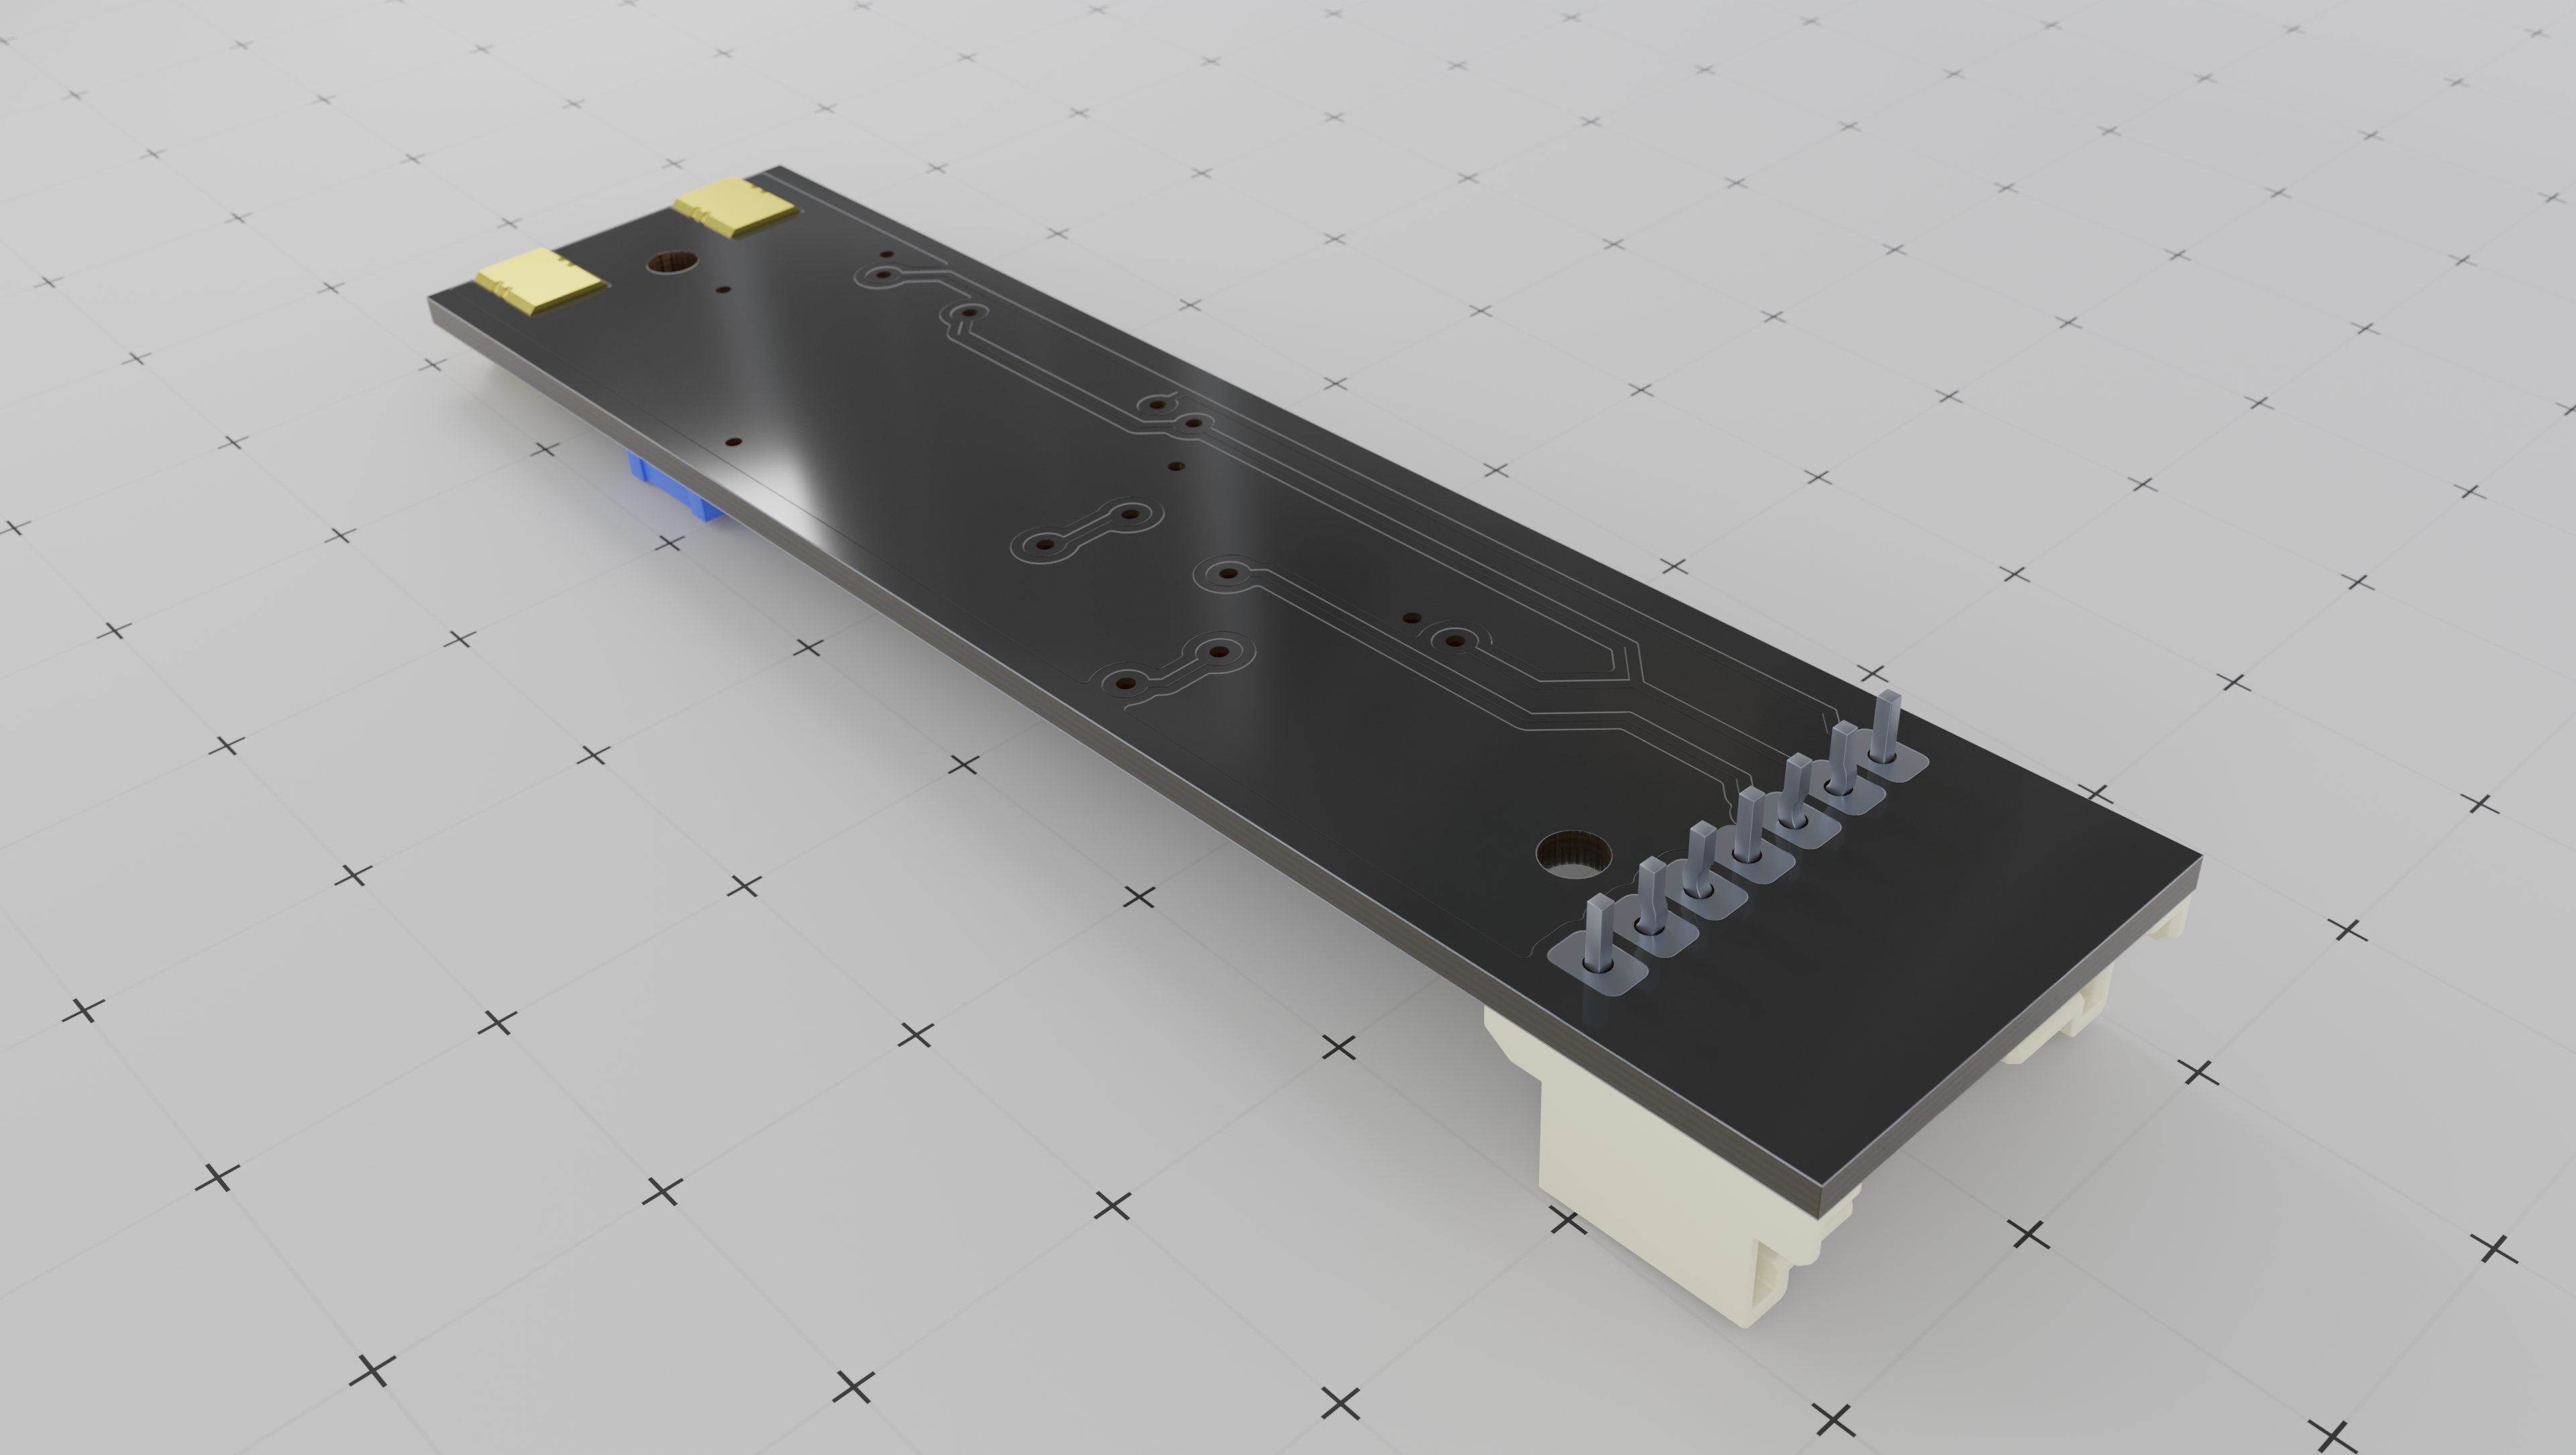
\includegraphics[width=\linewidth]{media/Render3.png}
                \end{minipage}
                \hspace{.04\linewidth}
                \begin{minipage}[H]{.45\linewidth}
                    \centering
                    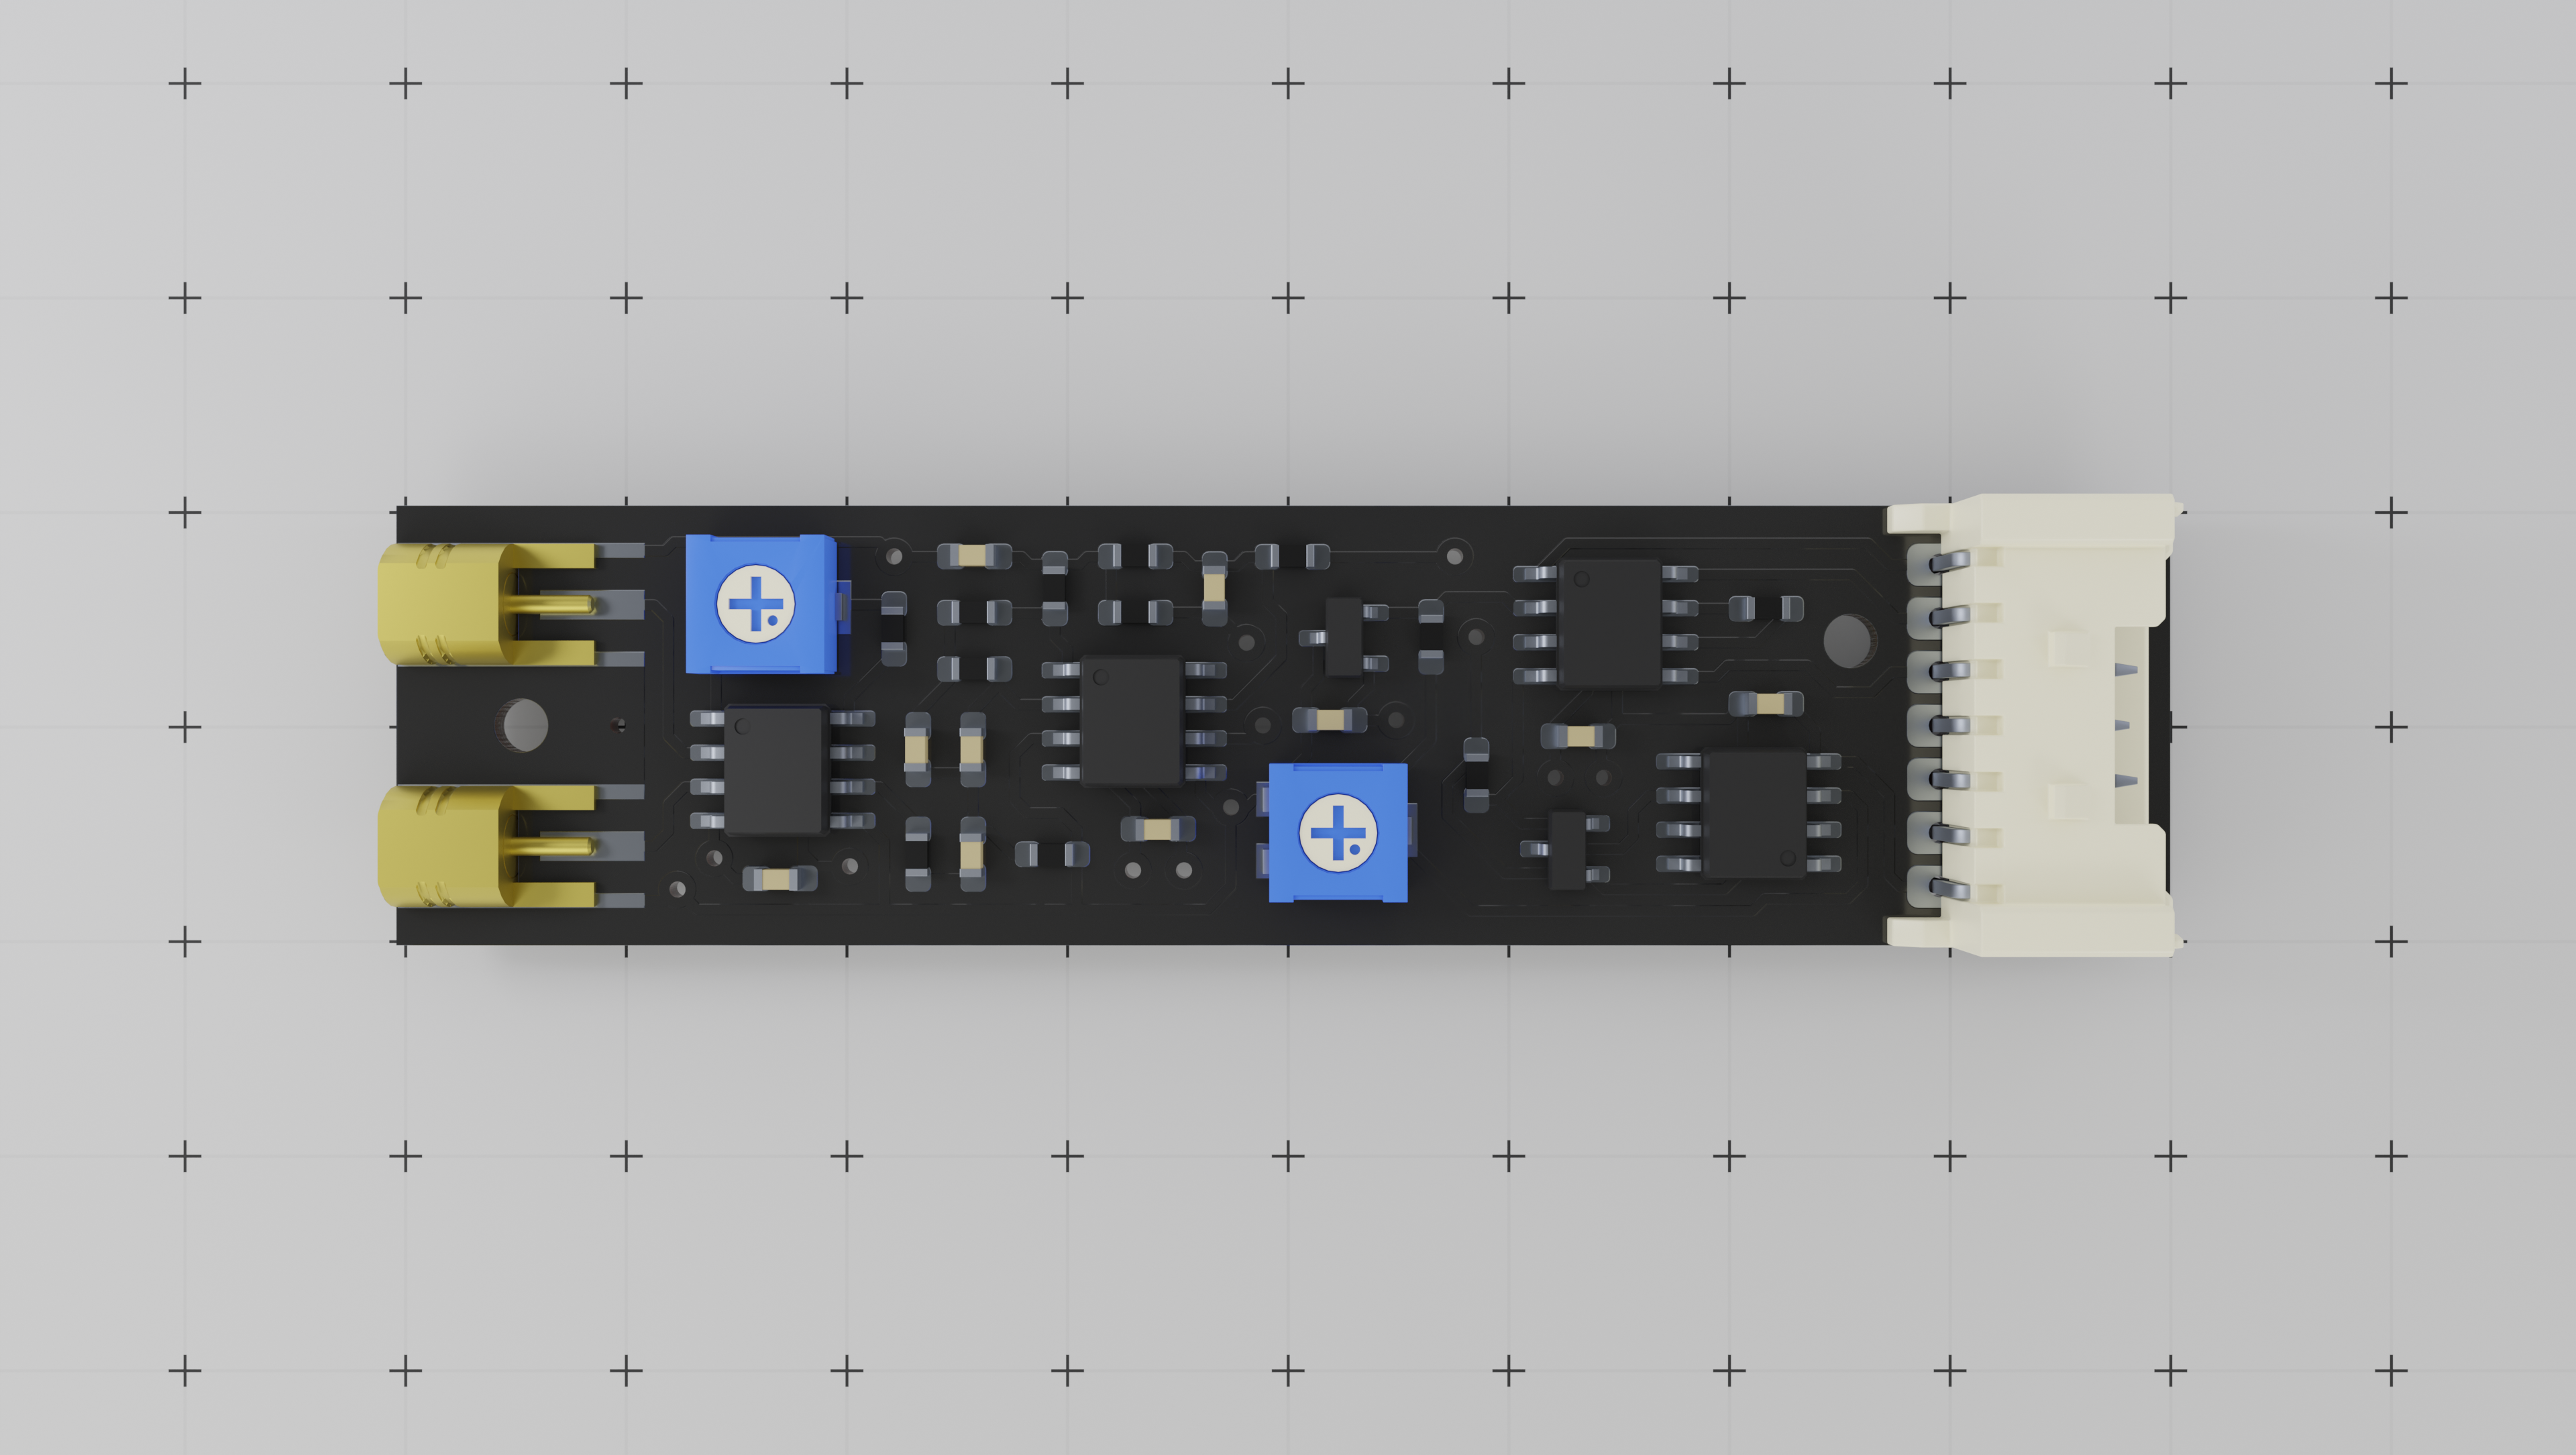
\includegraphics[width=\linewidth]{media/Render2.png}
                \end{minipage}
                \\
                \vspace*{.04\linewidth}
                \begin{minipage}[H]{.95\linewidth}
                    \centering
                    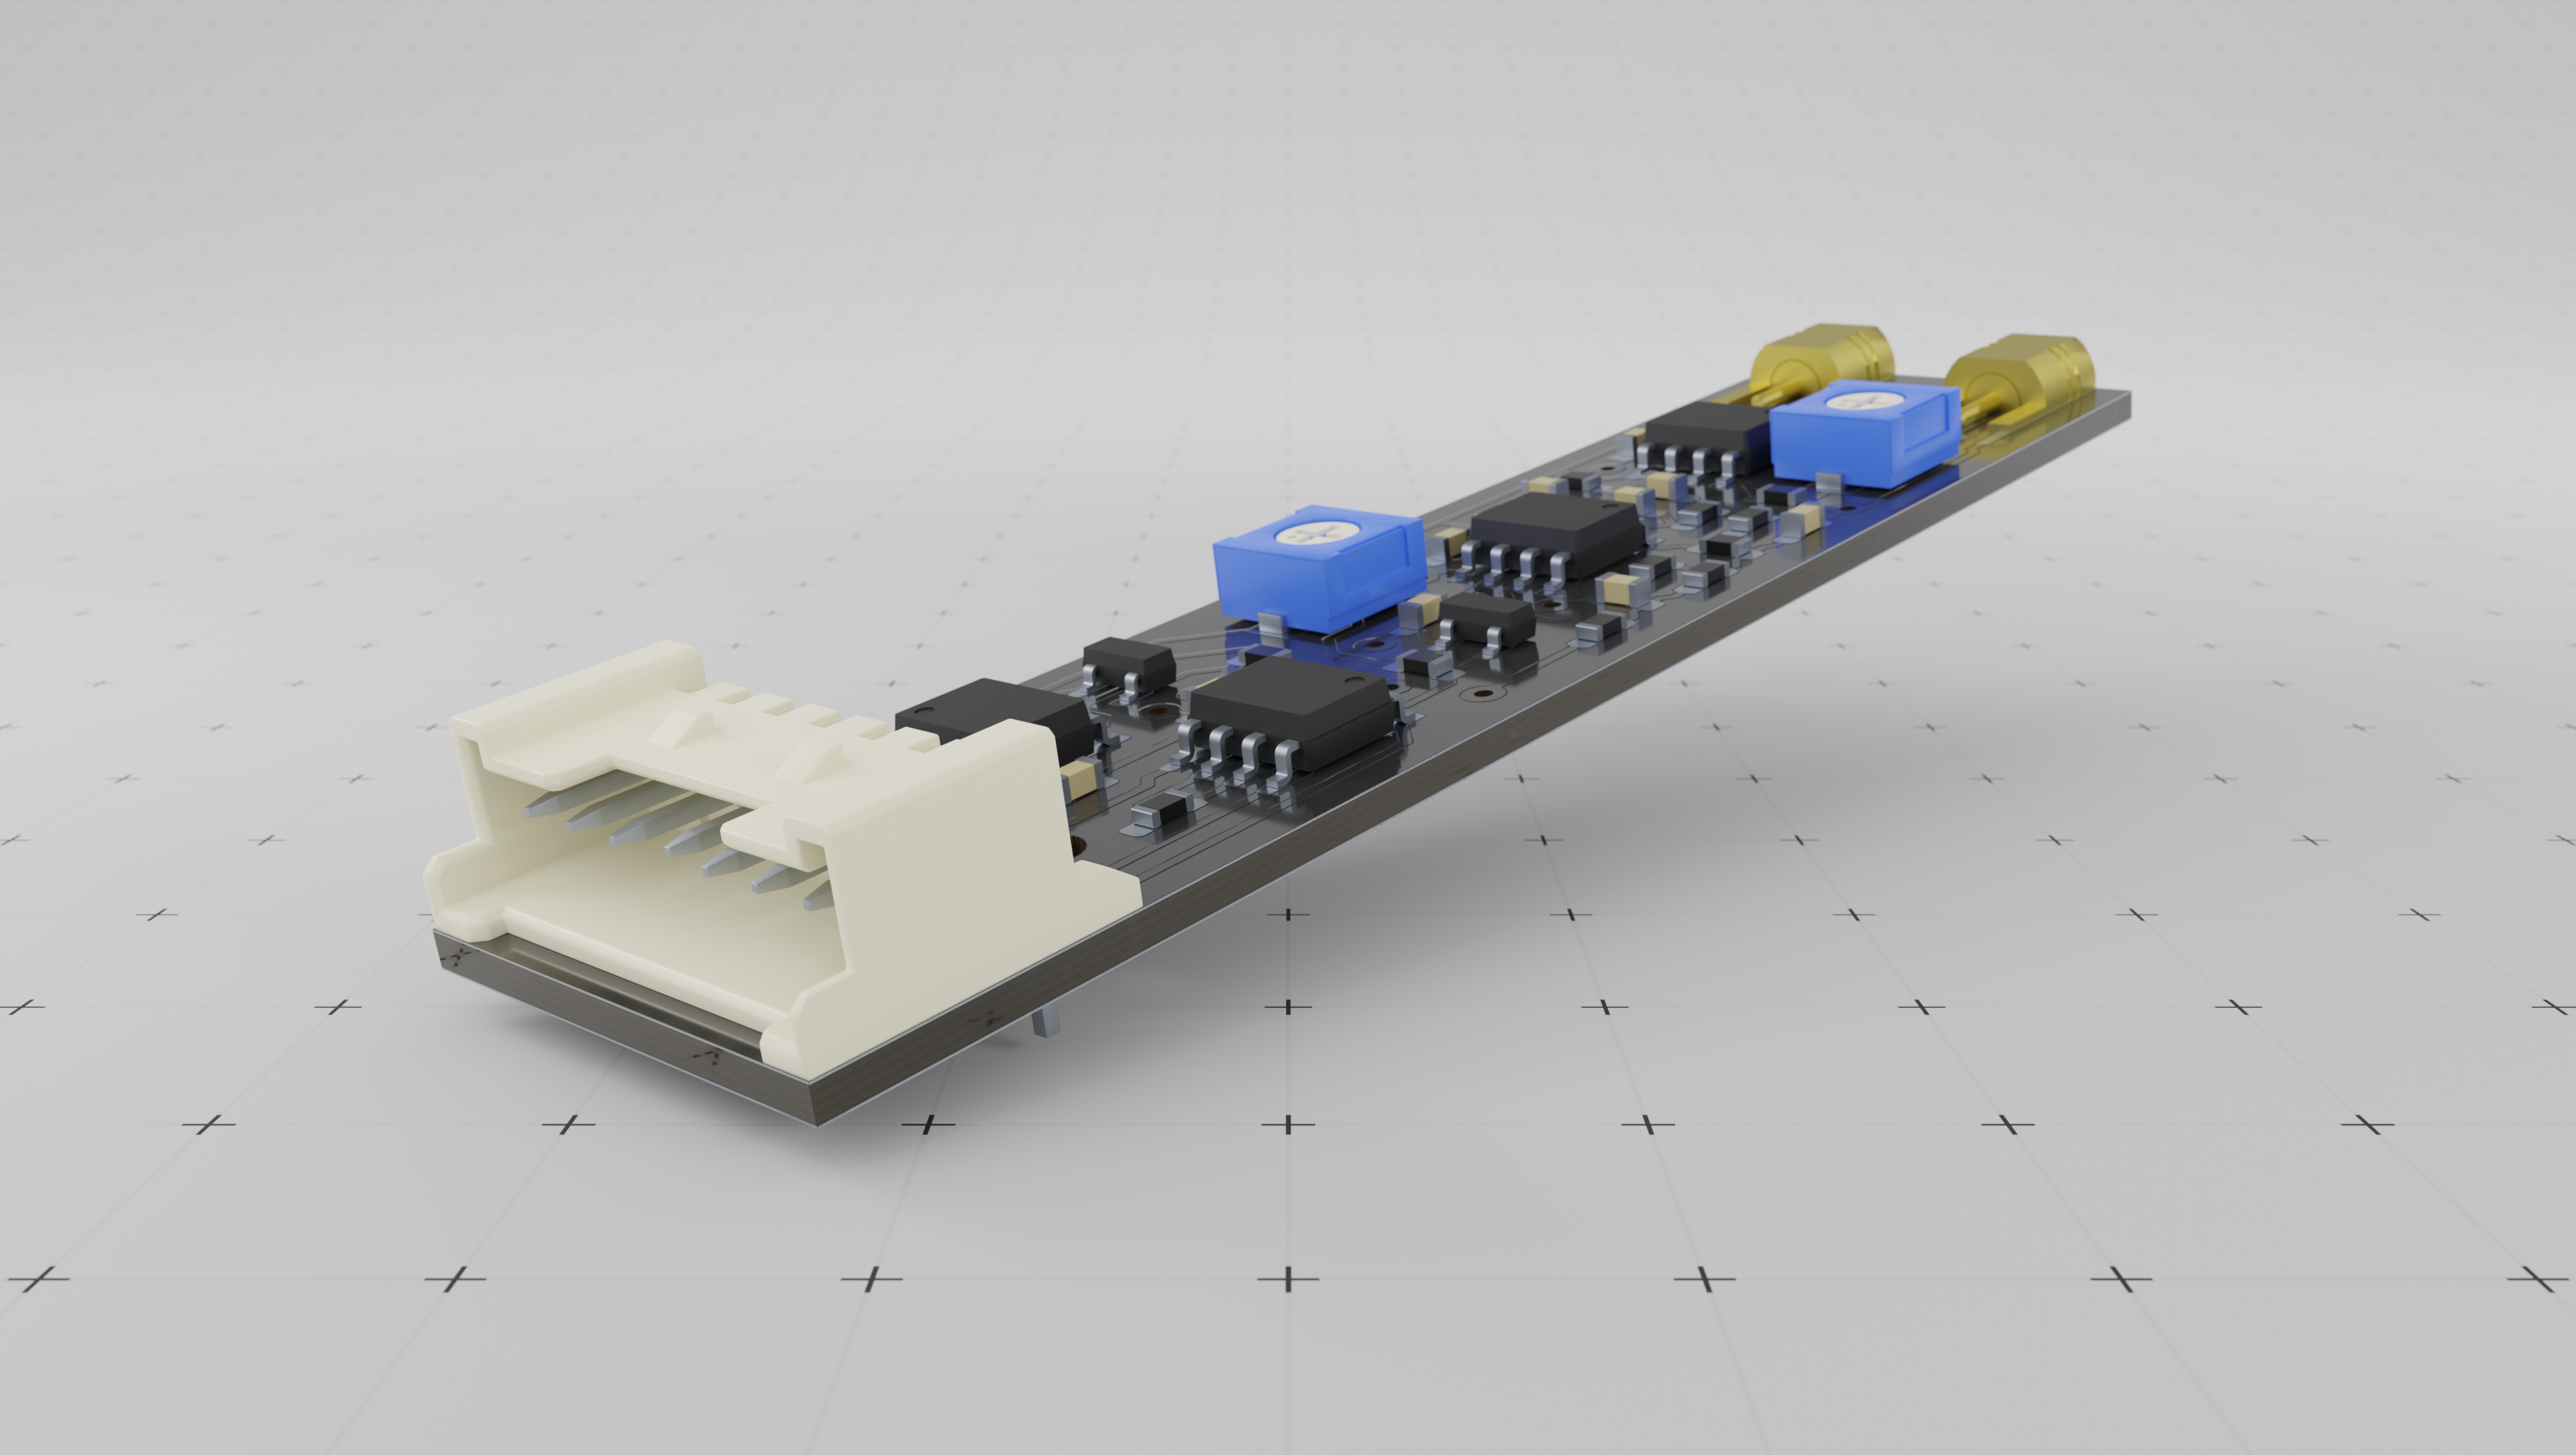
\includegraphics[width=\linewidth]{media/Render1.png}
                \end{minipage}
            \end{figure}
            
            \vspace*{\stretch{2}}
        \end{center}
    \end{titlepage}

    \clearpage
    % \listoftodos
    % \clearpage

    \section*{Abstract}
    \par Analog filters are an unavoidable\footnote{The impossibility of eliminating them is discussed in Section \ref{sec:ProjectDesignAbstractModel}, last list of 6 points}\todo{Check the number of points} and indispensable component of 21st-century technology: they are part of the internal components of electrical devices, starting from smartphones and ending with scientific measuring instruments.
    From the sources that can be found on the internet it is very complicated to extract the information needed to be able to make a practical and effective design of analog filters.
    Precisely for this reason there are many individuals among electronics enthusiasts who believe that designing filters is easy to do, that is, with a couple of formulas, which of course give some information, but what they leave out of consideration is covered by the person's sense of intuition.
    I, on the other hand, believe that this topic must be perfectly clear to everyone who considers themselves an electronics enthusiast.
    The main topic of this document is the design of analog filters not only at a theoretical level, but also at a practical level: at the end of the document a real board is presented that is able to detect extremely weak signals from the surface of the skin, amplify them and transmit them as data to the computer.
    The theory given is broad, but not too broad, just right to understand how filters work, how to design them and then build them.
    \clearpage
    \tableofcontents

    \clearpage
    \section{Introduction}\label{sec:Intro}
    \subsection{Motivation}\label{sec:IntroMotivation}
    Before starting work on the \emph{maturit\`{a}} thesis I began to notice more and more the lack of a private means of transport and I became interested in solving the problem.
    Taking into account the budget, the desired quality and the specific characteristics: portability, reduced size and weight, repairability and the possibility of replacing a means of transport, I chose to build an electric skateboard.
    
    One issue I dwelt on most was the remote control, because the skateboard requires control by the person riding it.
    Looking into it, I discovered that currently\footnote{During the year 2021} on the technology market, electric skateboards have fairly simple remote controls, equipped with buttons together with some analog variant\footnote{With more than two states} to be able to dose the power with which the motors are driven.
    So I decided\footnote{The factors that influenced the choice will be explained in Section \ref{sec:IntroReader}} to adopt a much less standard idea which, moreover, appears to me to be either new or rarely used: the concept of gesture control in combination with a means of transport.
    
    By a convenient coincidence of dates, during the development of the project I also needed to do a \emph{maturit\`{a}} thesis on a robotics topic, that is, also physics and mathematics, which involved building a robotic prototype based on personal studies and research. Naturally, I tried to keep the ongoing project, which unfortunately, taken as a whole, was excessively broad for a \emph{maturit\`{a}} thesis. So, guided by the appeal of creating a device that would not occupy the hand during use\footnote{During a fall or any unforeseen situation the immediate availability of the hands is desirable, and moreover I believe it increases comfort} and by my own opinion of the originality of the idea, I decided to present a small part of it: the analog part of the electromyographic sensor\footnote{The terms and the reasons for the choice will be clarified in Section \ref{sec:IntroReader}}, and later\footnote{Section \ref{sec:IntroMotivation}} it will become clear that it is mainly a filter.
    
    \subsection{Aim of the work}\label{sec:IntroAim}
    \noindent The aim of this \emph{maturit\`{a}} thesis is:
    \begin{enumerate}[label=\emph{(\roman*)}]
        \item To introduce the reader to the concept of filters and how they work in terms of signals
        \item To provide the terminology concerning them
        \item To answer questions that arose during the development of the project
        \item To bring to attention the considerations to take into account during theoretical and practical design
        \item To build a prototype as a proof of concept
    \end{enumerate}
    Moreover, much of the knowledge given in the \emph{maturit\`{a}} thesis is applicable in various other fields, for example: the mathematical model of filters is fully valid for digital filters as well, and the practical details\footnote{As in Section \ref{sec:BuildingHardware}} \todo{add part on bypass capacitors, inductance, ground plane and skin effect} on circuit design are applicable to almost any other type of precision circuit.
    
    The content also includes the reasoning\footnote{A detailed reasoning on the motives that lead to the use of a filter, and the consequences that their use implies} preceding the filter development process, which helps to integrate the filter into a project, instead of isolating the concept and leaving crucial questions unanswered that may arise while working on a future project.
    
    \subsection{Organization of the work}\label{sec:IntroOrganization}
    The specific characteristics of the project, such as the project management\footnote{The term and the characteristic it denotes will be discussed in Section \ref{sec:ProjectCharacteristics}} methods used and the size of the project compared to the part of it presented in the \emph{maturit\`{a}} thesis, dictate some rules for organizing the project, which I discuss in this Section.
    If the process dictated by the methods and by the complexity of the project were documented chronologically, the written content would turn out too long, poorly consistent with the topic of the \emph{maturit\`{a}} thesis and often confusing.
    
    \begin{samepage}
        \noindent The scheme I follow while documenting the whole \emph{maturit\`{a}} thesis to solve the organizational problems is the following:
        \begin{enumerate}[label=\emph{(\roman*)}]
            \item Theory \& Practice
            \item Characteristics
            \item Design
        \end{enumerate}
    \end{samepage}
    It is worth noting that this three-part scheme does not try to shape the whole \emph{maturit\`{a}} thesis in the style of "\emph{Introduction}", "\emph{Main body}", "\emph{Conclusions}", but attempts to rearrange the contents into conceptual groups in order to then build on them a cohesive discussion, with a steady and logical flow, while not denying the presence of the main scheme as the "de facto"\footnote{Taken as a formal standard because it is obvious to a large number of people} standard just mentioned.
    
    The \emph{Theory \& Practice} part serves to give the reader the information needed to grasp the topics touched on in the following parts.
    The \emph{Characteristics} part serves to understand what characteristics the subject must have or has, and which of them influence the next part and the subsequent hierarchically subordinate subjects.
    The \emph{Design} part is where the choices made are motivated and asserted through reasoning; they are always closely connected to the previous parts of the same subject and of the preceding subjects.
    Of course, the \emph{Characteristics} and \emph{Design} parts contain theoretical and practical parts, but when the information under consideration becomes too extensive to describe in one Section, it is grouped into a separate \emph{Theory \& Practice} Section placed before the two.
    
    \begin{samepage}
        \noindent An example could be:
        \begin{enumerate}[label=\emph{(\roman*)}]
            \item Section \ref{sec:IntroFiltersSignals} $\Rightarrow$ \emph{Theory \& Practice}
            \item Section \ref{sec:ProjectCharacteristics} $\Rightarrow$ \emph{Characteristics}
            \item Section \ref{sec:ProjectDesign} $\Rightarrow$ \emph{Design}
        \end{enumerate}
    \end{samepage}

    \subsection{Introduction to the work}\label{sec:IntroReader}
    To introduce the reader to the \emph{maturit\`{a}} thesis, in this Section I explain some basic concepts needed to follow the discussion, and I report in condensed form the reasoning that belongs to the part of the work done before reaching the sensor development stage.

    Between theory and practice, I prefer to start from the theoretical part to show the reader a simple model that can be developed, extended and refined over the course of the reading.
    
    Generalizing as much as possible, the problem being solved is the transmission of information over a short distance.
    I considered that the only logical choice through which to look for the solution would be electronics, because of the possibility of creating compact devices and of transmitting information via RF\footnote{Radio frequencies}, which are by definition a feature of the phenomenon of electromagnetism\footcite["The" (electromagnetic) "field can be viewed as the combination of an electric field and a magnetic field"]{Electromagnetism:Wiki} \footcite["Electricity is related to magnetism, both being part of the phenomenon of electromagnetism"]{Electricity:Wiki}.
    I then applied an abstraction technique with the help of an analogy to \emph{Input/Output} \footcite[]{IO:Wiki}.
    It consists of understanding which possible "\emph{Outputs}\footnote{Information outlets}" the subject from which information is to be collected has, what they would cause from a physical point of view, and finally choosing some phenomena to then convert into feedback\footnote{Return signal}, in our case electrical feedback.
    In the case of a human as the subject, only the \emph{movement} of the person or of their body parts and the production of \emph{sounds} \footnote{Voice, hand clapping, whistling, etc...} can allow information to be expressed.
    I chose to transmit information through movements precisely so as not to interfere with sounds, to avoid possible interference\footnote{It is also possible with movements, but it is objectively rarer, given that sounds can spread through the air} and because there is little need for an excessively complex vocabulary\footnote{Said with regard to voice control}.
    The movements can be of any kind, such as shifting the body weight forward or backward relative to the vehicle, which however turned out to lack sufficient granularity of control and to interfere with the use of the vehicle\footnote{One needs an ideal sense of balance to keep control during moments such as acceleration and braking}.
    \clearpage  
    \noindent Since no other movement seemed comfortable enough, the last remaining possibility was the hand, which proved to be very effective because of its granularity of control and flexibility.
    Applying the technique just mentioned\footnote{Technique used with the Input/Output analogy} a second time,
    there were different ideas for possible variations of the "\emph{Output}" of the subject\footnote{Input/Output analysis of the hand} \emph{(indicated by numbers)} and ideas for solutions to exploit them \emph{(indicated by letters)}:
    \begin{enumerate}[label=\emph{(\arabic*)}]
        \item Change in the position of the fingers and of the hand
            \begin{enumerate}[label=\emph{(\alph*)}]
                \item Glove with rotary encoders\footnote{Rotational encoder} \footnote{There are different types of rotary encoder: contact, optical, Hall-effect (magnetic)}\emph{(Figure \ref{fig:IdeaEncoderGlove})} with springs and wires, or flex sensors\footnote{Bend sensors} \footnote{They change their resistance depending on how much they are bent}\emph{(Figure \ref{fig:IdeaFlexGlove})}
                \item Bracelet with an electromagnetic radar such as the "Soli" chip\footcite[]{GoogleATAP:Wiki} \emph{(Figure \ref{fig:IdeaRadarGlove})}
                \item MEMS sensors\footnote{Combination of gyroscope, accelerometer and sometimes sensors of the Earth's magnetic field to precisely identify the position in space} on each finger and on the hand \emph{(Figure \ref{fig:IdeaMEMSGlove})}
            \end{enumerate}
        \item Change in muscle diameter due to contraction
        \item Change in the electric field in the nerve due to the signal it carries, and consequently also in the muscle due to its contraction \label{ItemDeltaChoice}
            \begin{enumerate}[label=\emph{(\alph*)}]
                \item Needle electrodes \emph{(Figure \ref{fig:IdeaNeedleEMGBand})}, surface-contact or surface-capacitive electrodes \emph{(Figure \ref{fig:IdeaSurfaceEMGBand})}, which are subject to changes in electric charge due to the electromagnetic fields generated by the muscle and/or the nerve \label{ItemEMG}
            \end{enumerate}
    \end{enumerate}

    \begin{figure}[H]
        \centering
        \begin{minipage}[H]{.32\linewidth}
            \centering
            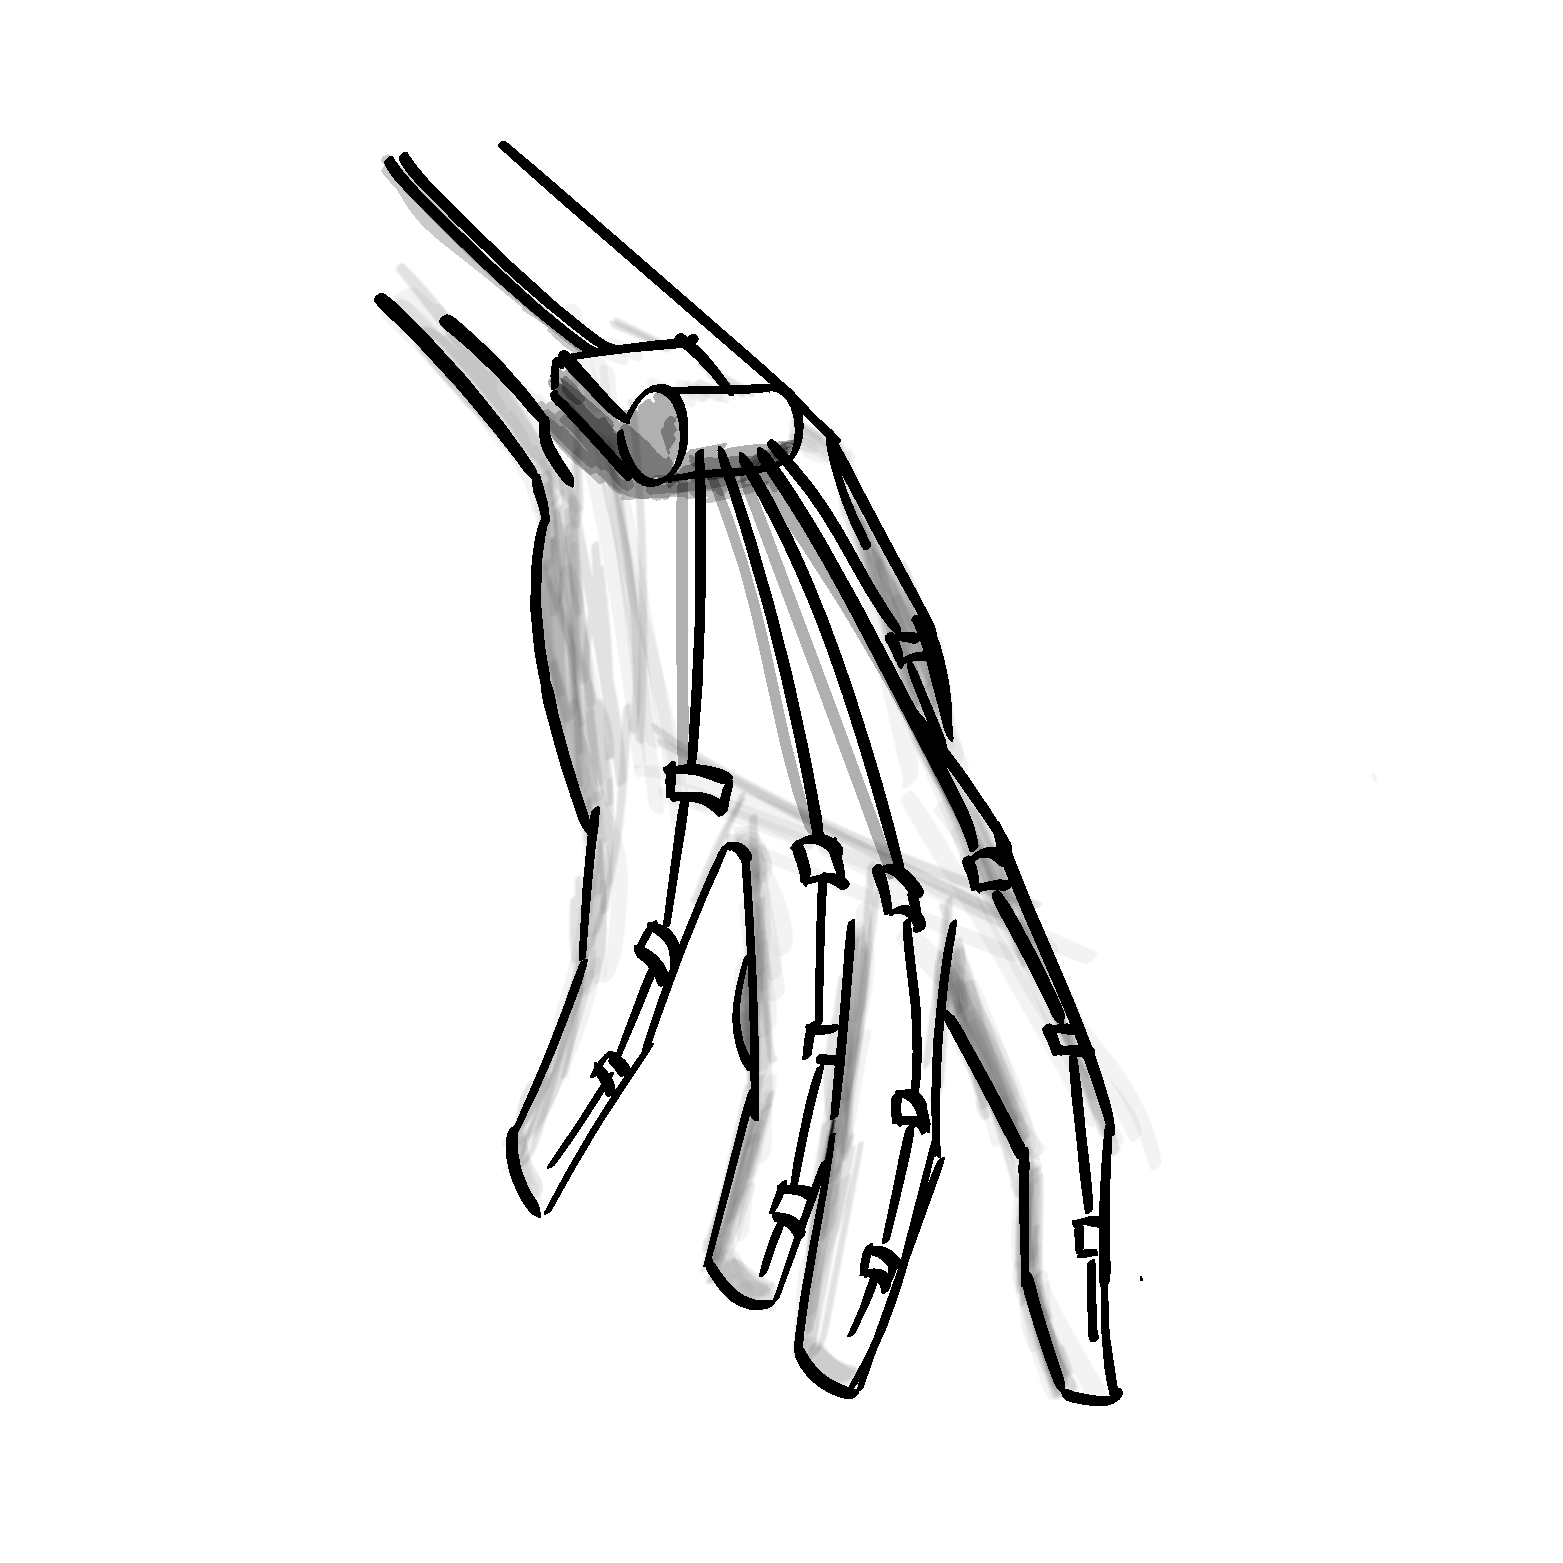
\includegraphics[page=1, width=\linewidth]{media/Ideasheet1.pdf}
            \subcaption{}\label{fig:IdeaEncoderGlove}
        \end{minipage}
        \begin{minipage}[H]{.32\linewidth}
            \centering
            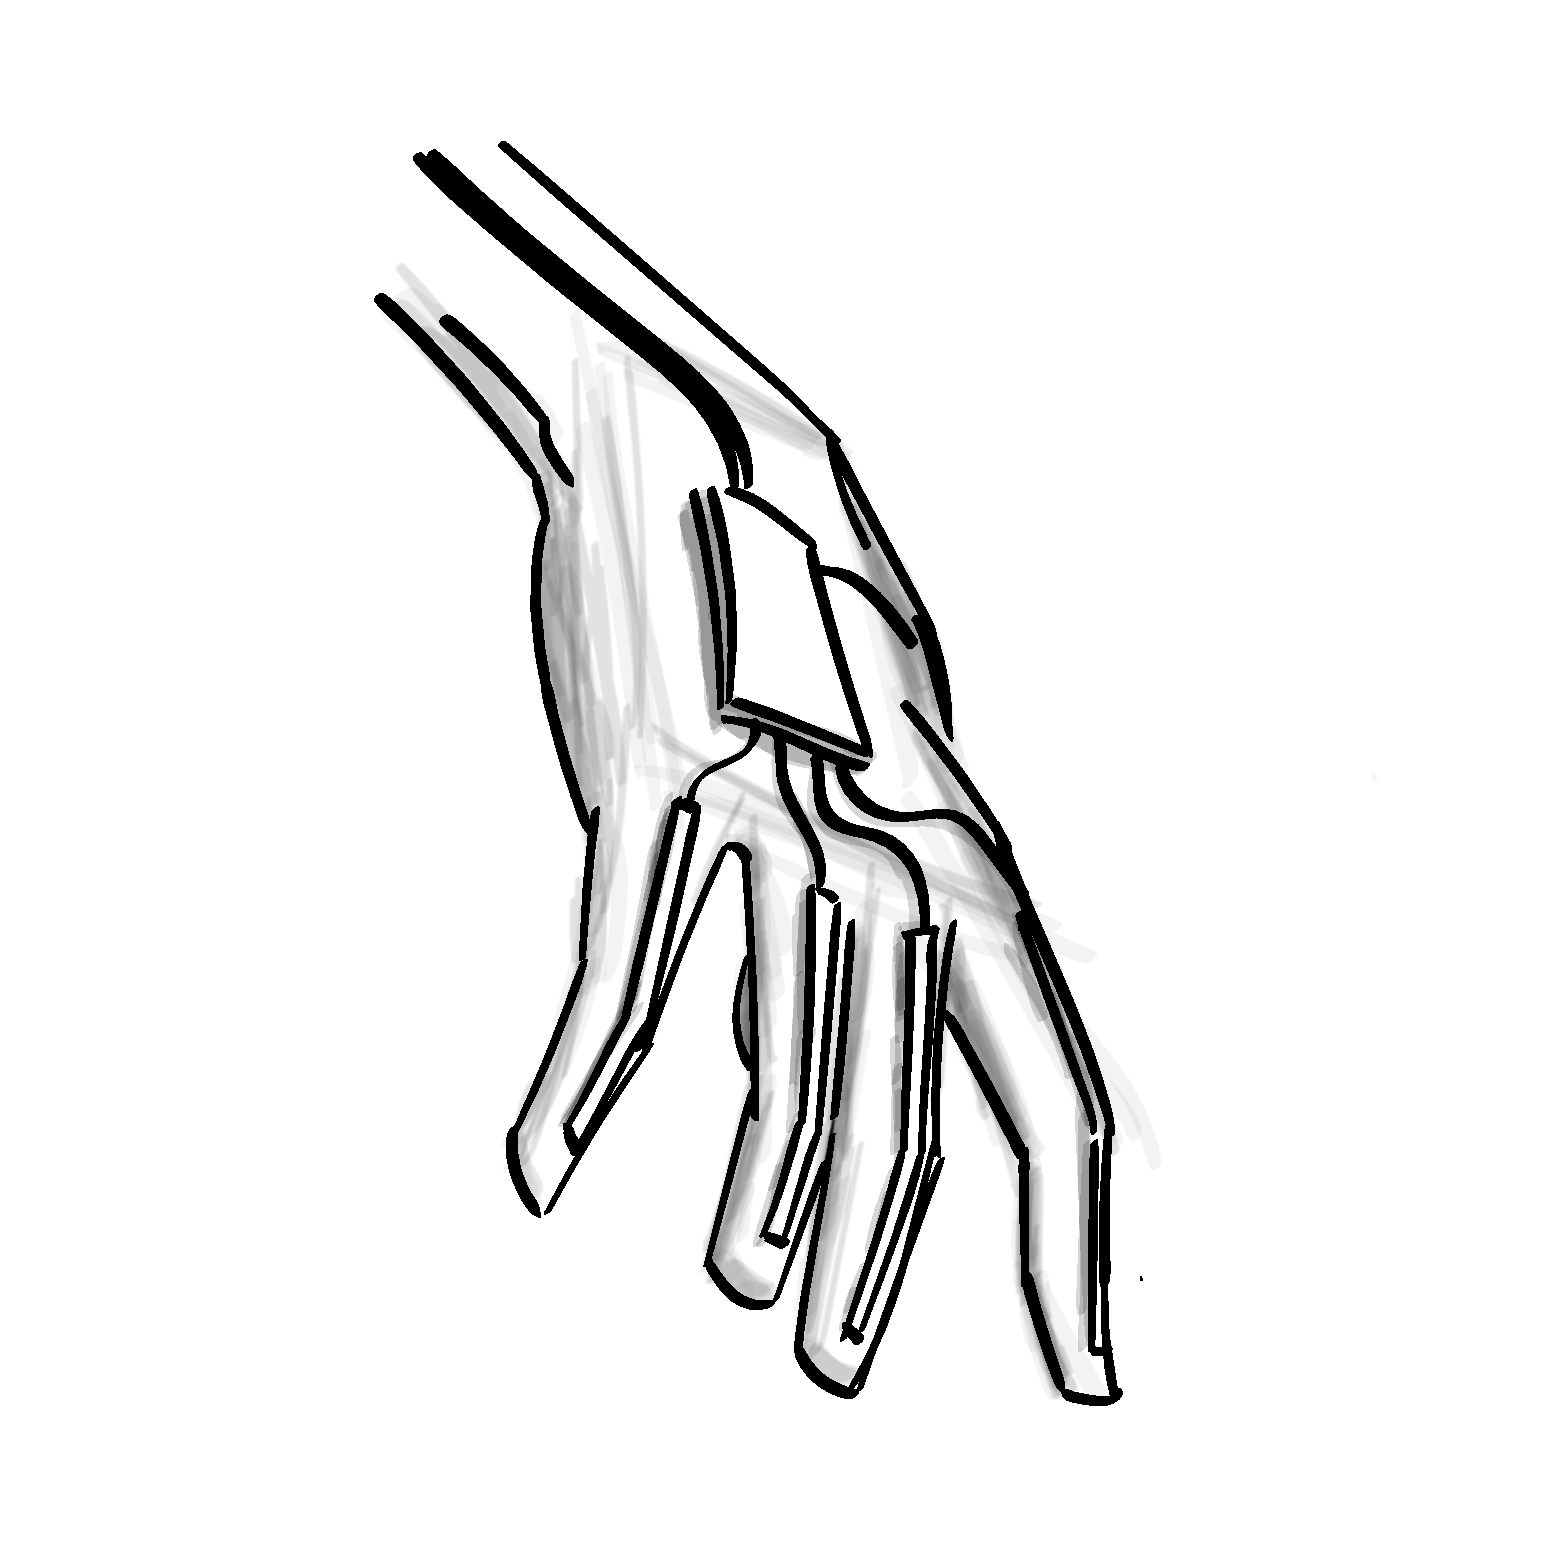
\includegraphics[page=1, width=\linewidth]{media/Ideasheet2.pdf}
            \subcaption{}\label{fig:IdeaFlexGlove}
        \end{minipage}
        \begin{minipage}[H]{.32\linewidth}
            \centering
            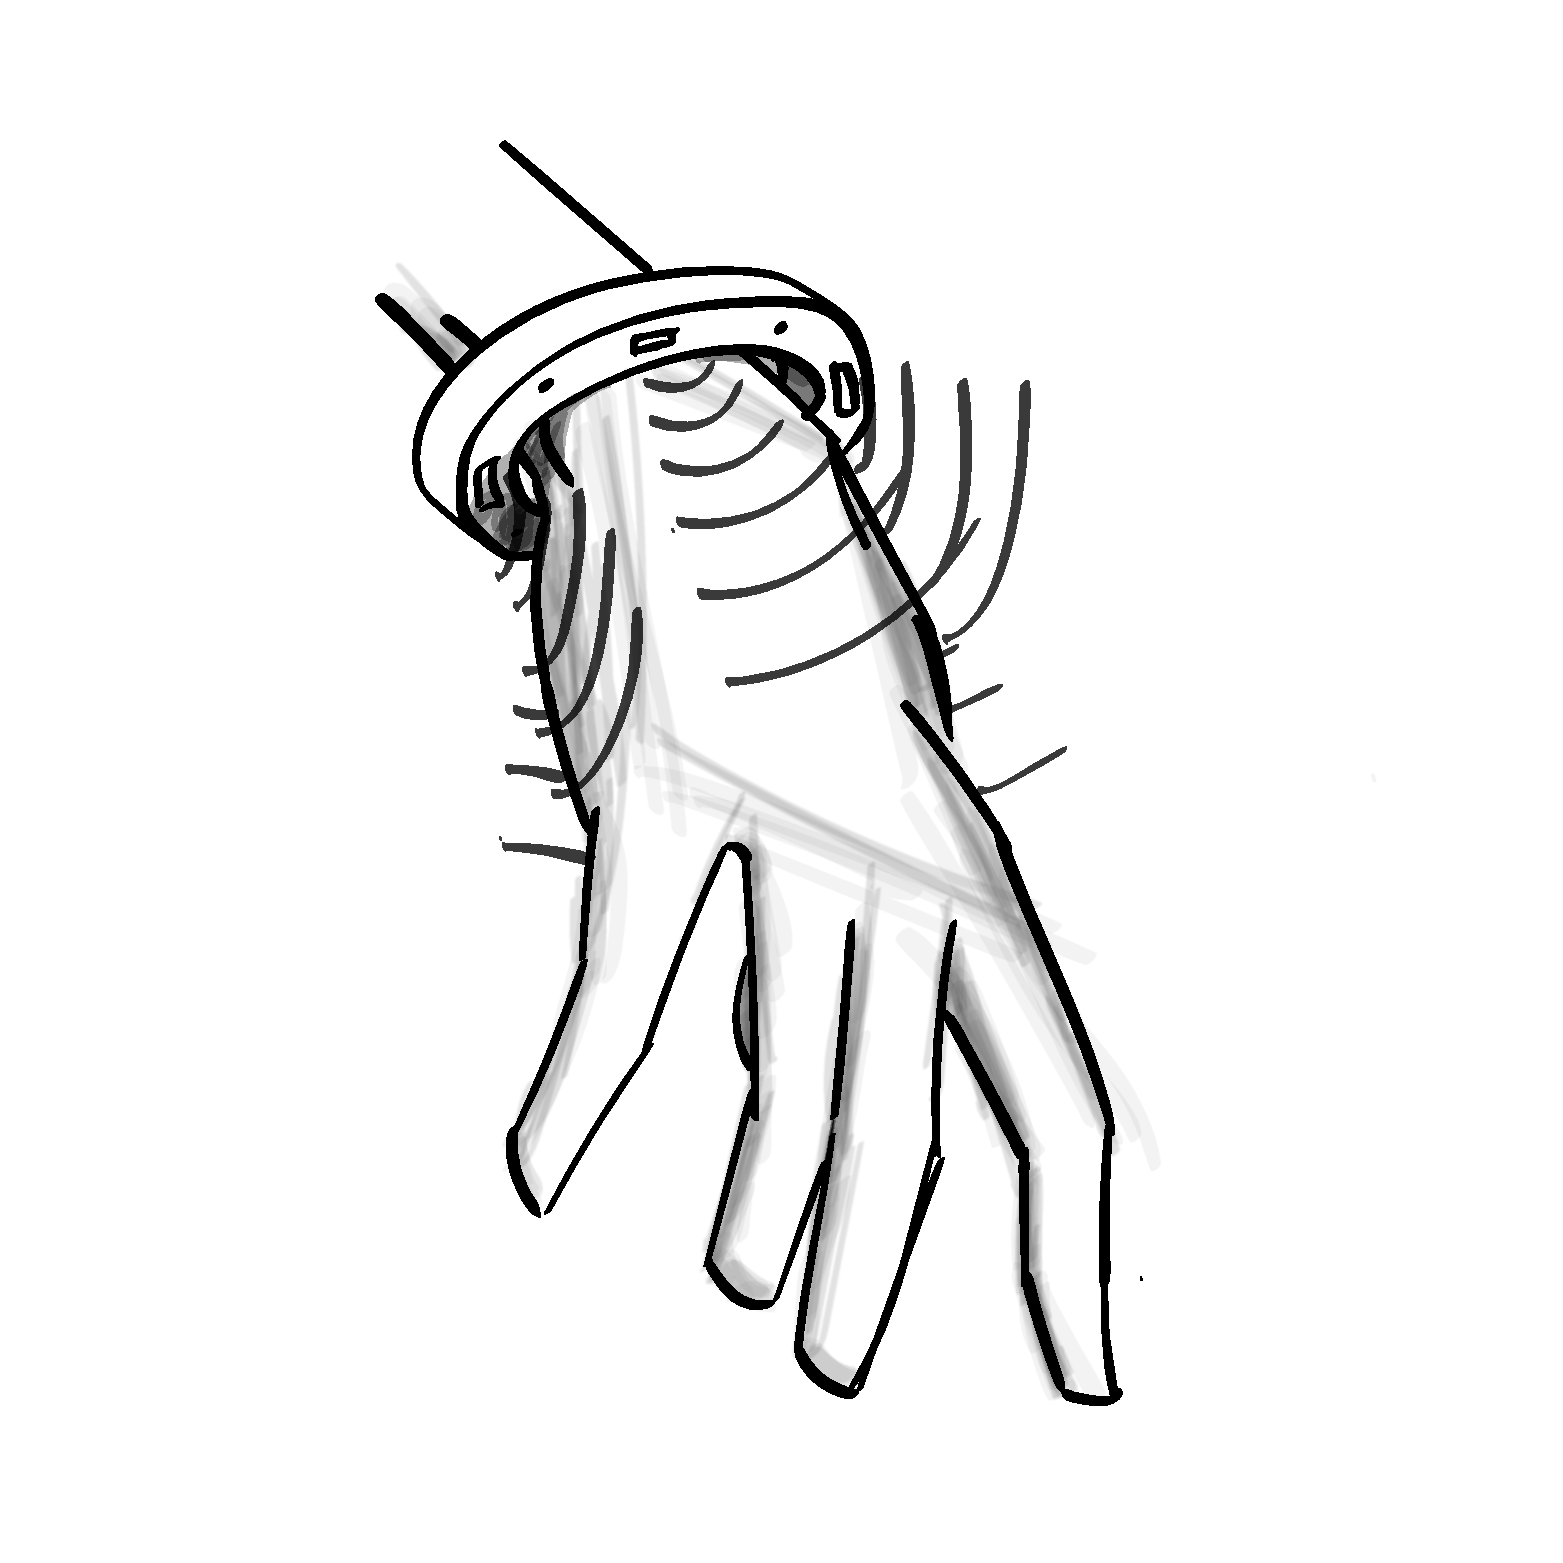
\includegraphics[page=1, width=\linewidth]{media/Ideasheet3.pdf}
            \subcaption{}\label{fig:IdeaRadarGlove}
        \end{minipage}
        \begin{minipage}[H]{.32\linewidth}
            \centering
            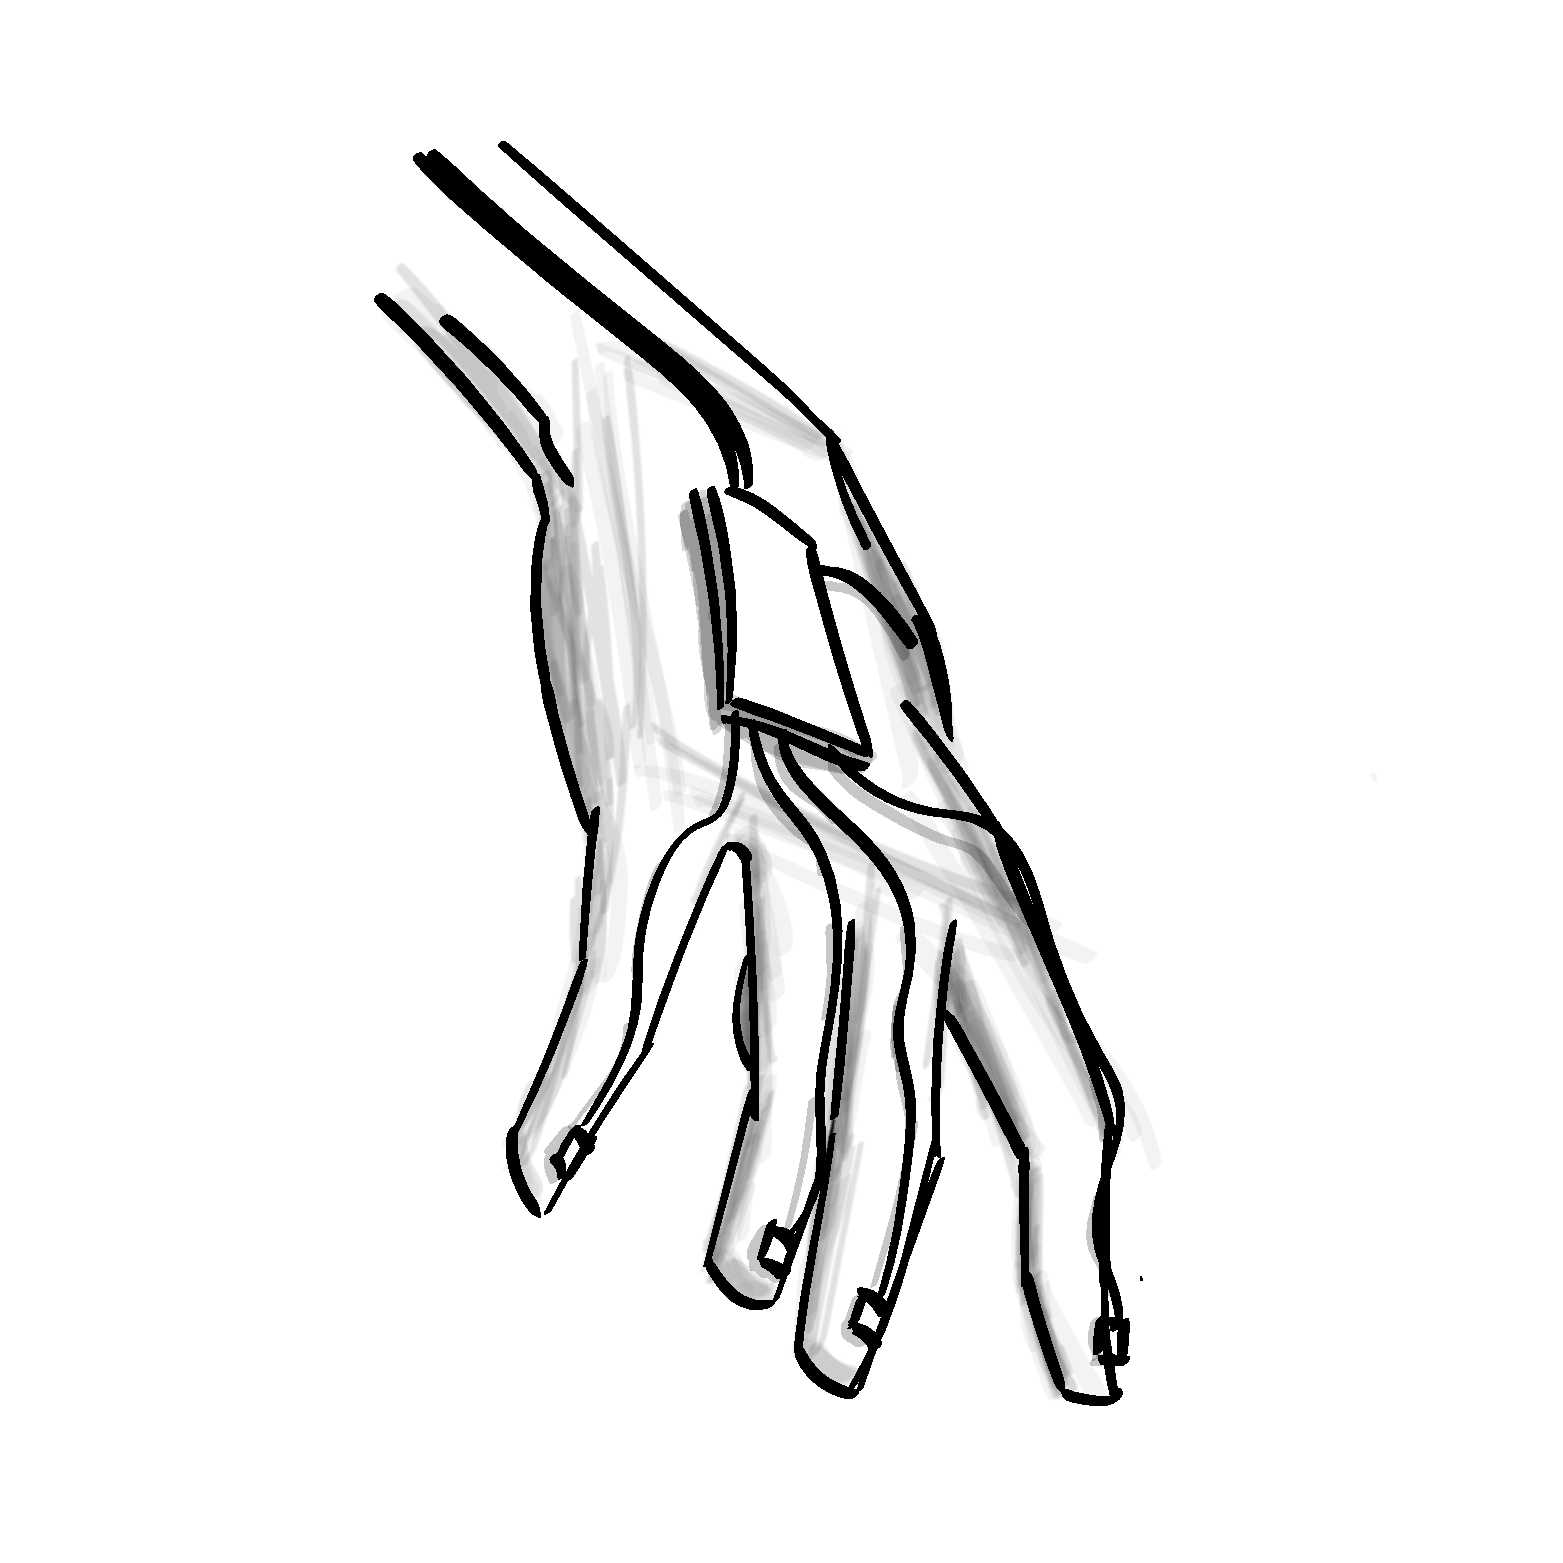
\includegraphics[page=1, width=\linewidth]{media/Ideasheet4.pdf}
            \subcaption{}\label{fig:IdeaMEMSGlove}
        \end{minipage}
        \begin{minipage}[H]{.32\linewidth}
            \centering
            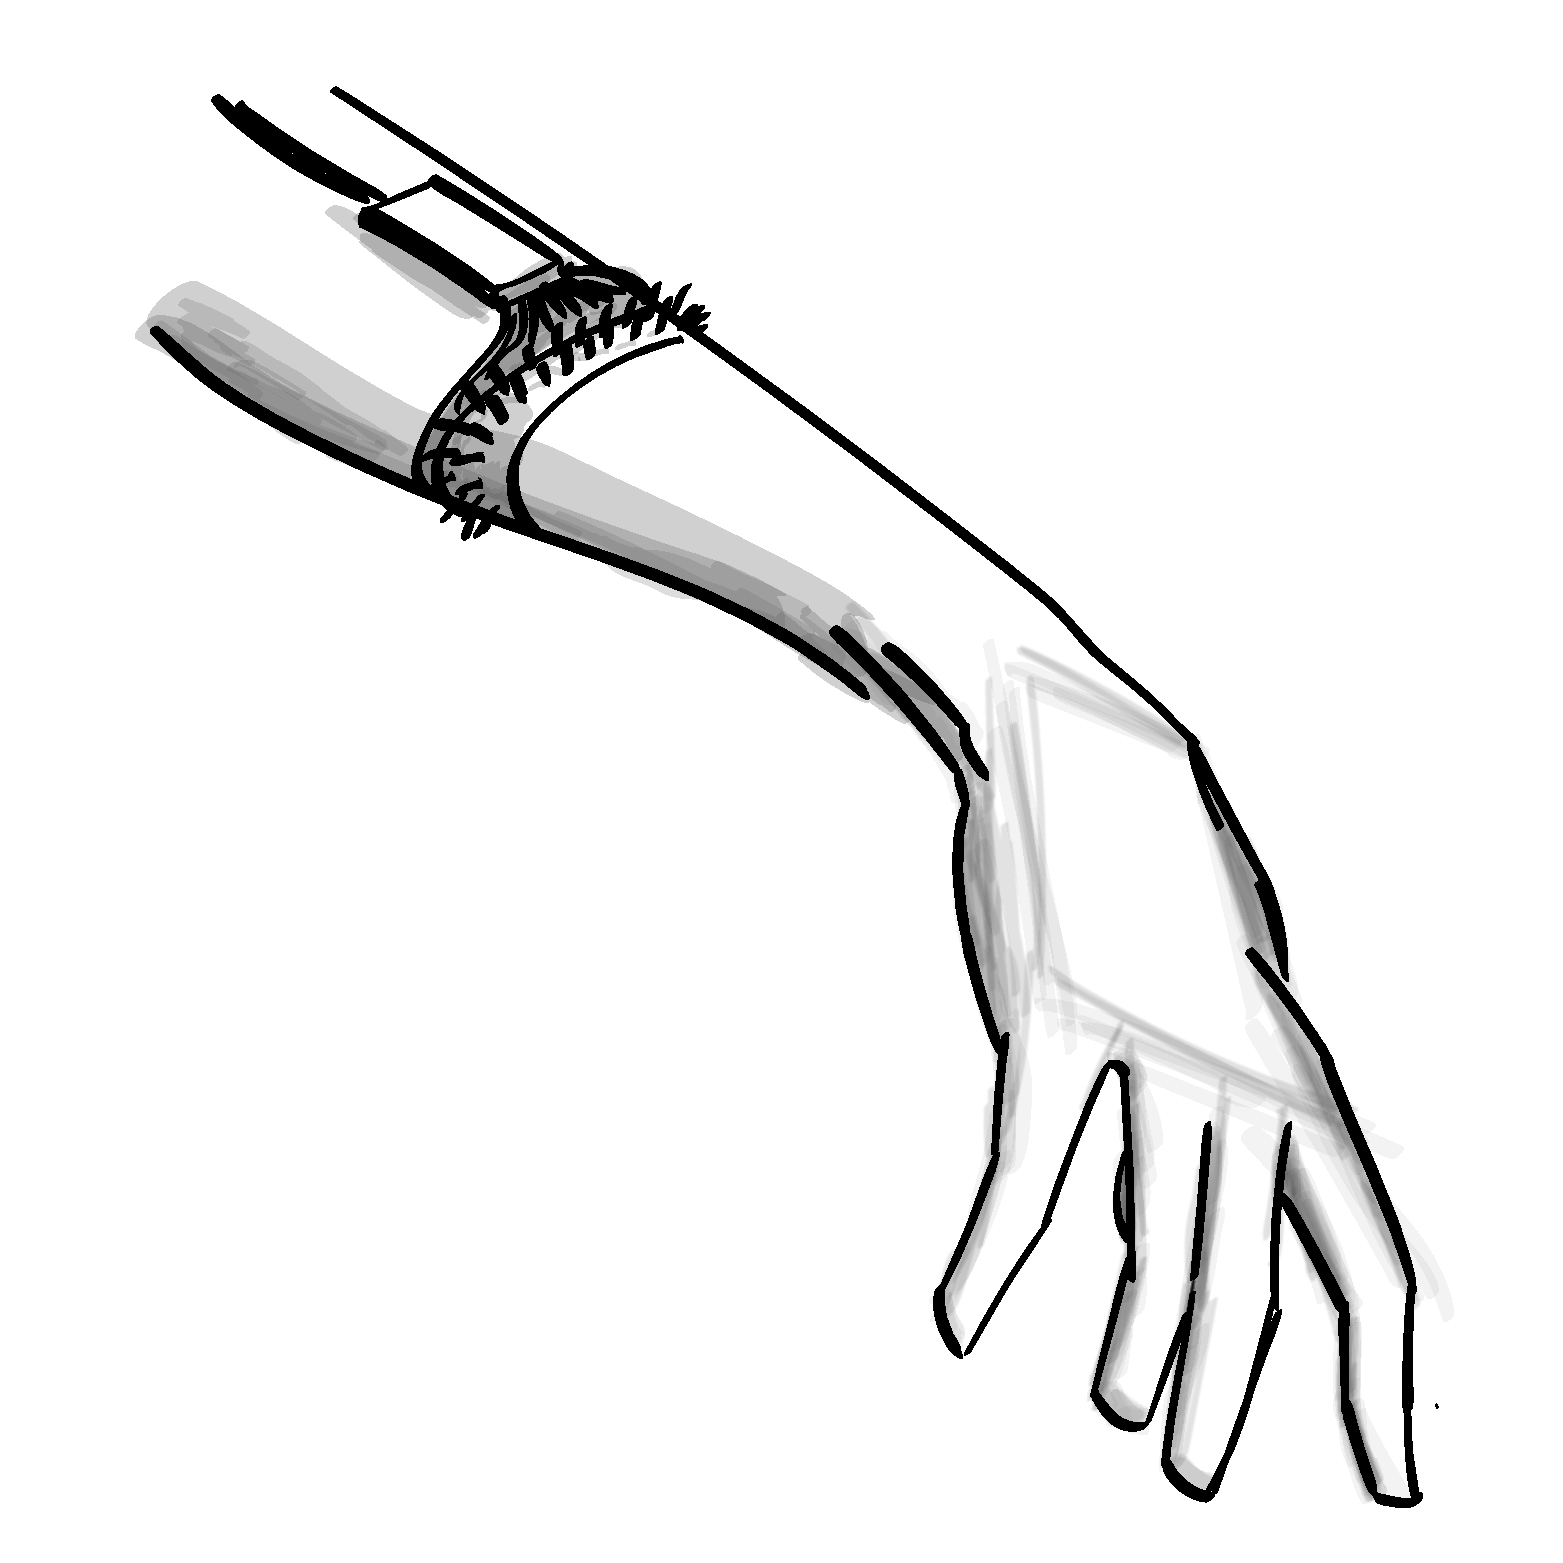
\includegraphics[page=1, width=\linewidth]{media/Ideasheet5.pdf}
            \subcaption{}\label{fig:IdeaNeedleEMGBand}
        \end{minipage}
        \begin{minipage}[H]{.32\linewidth}
            \centering
            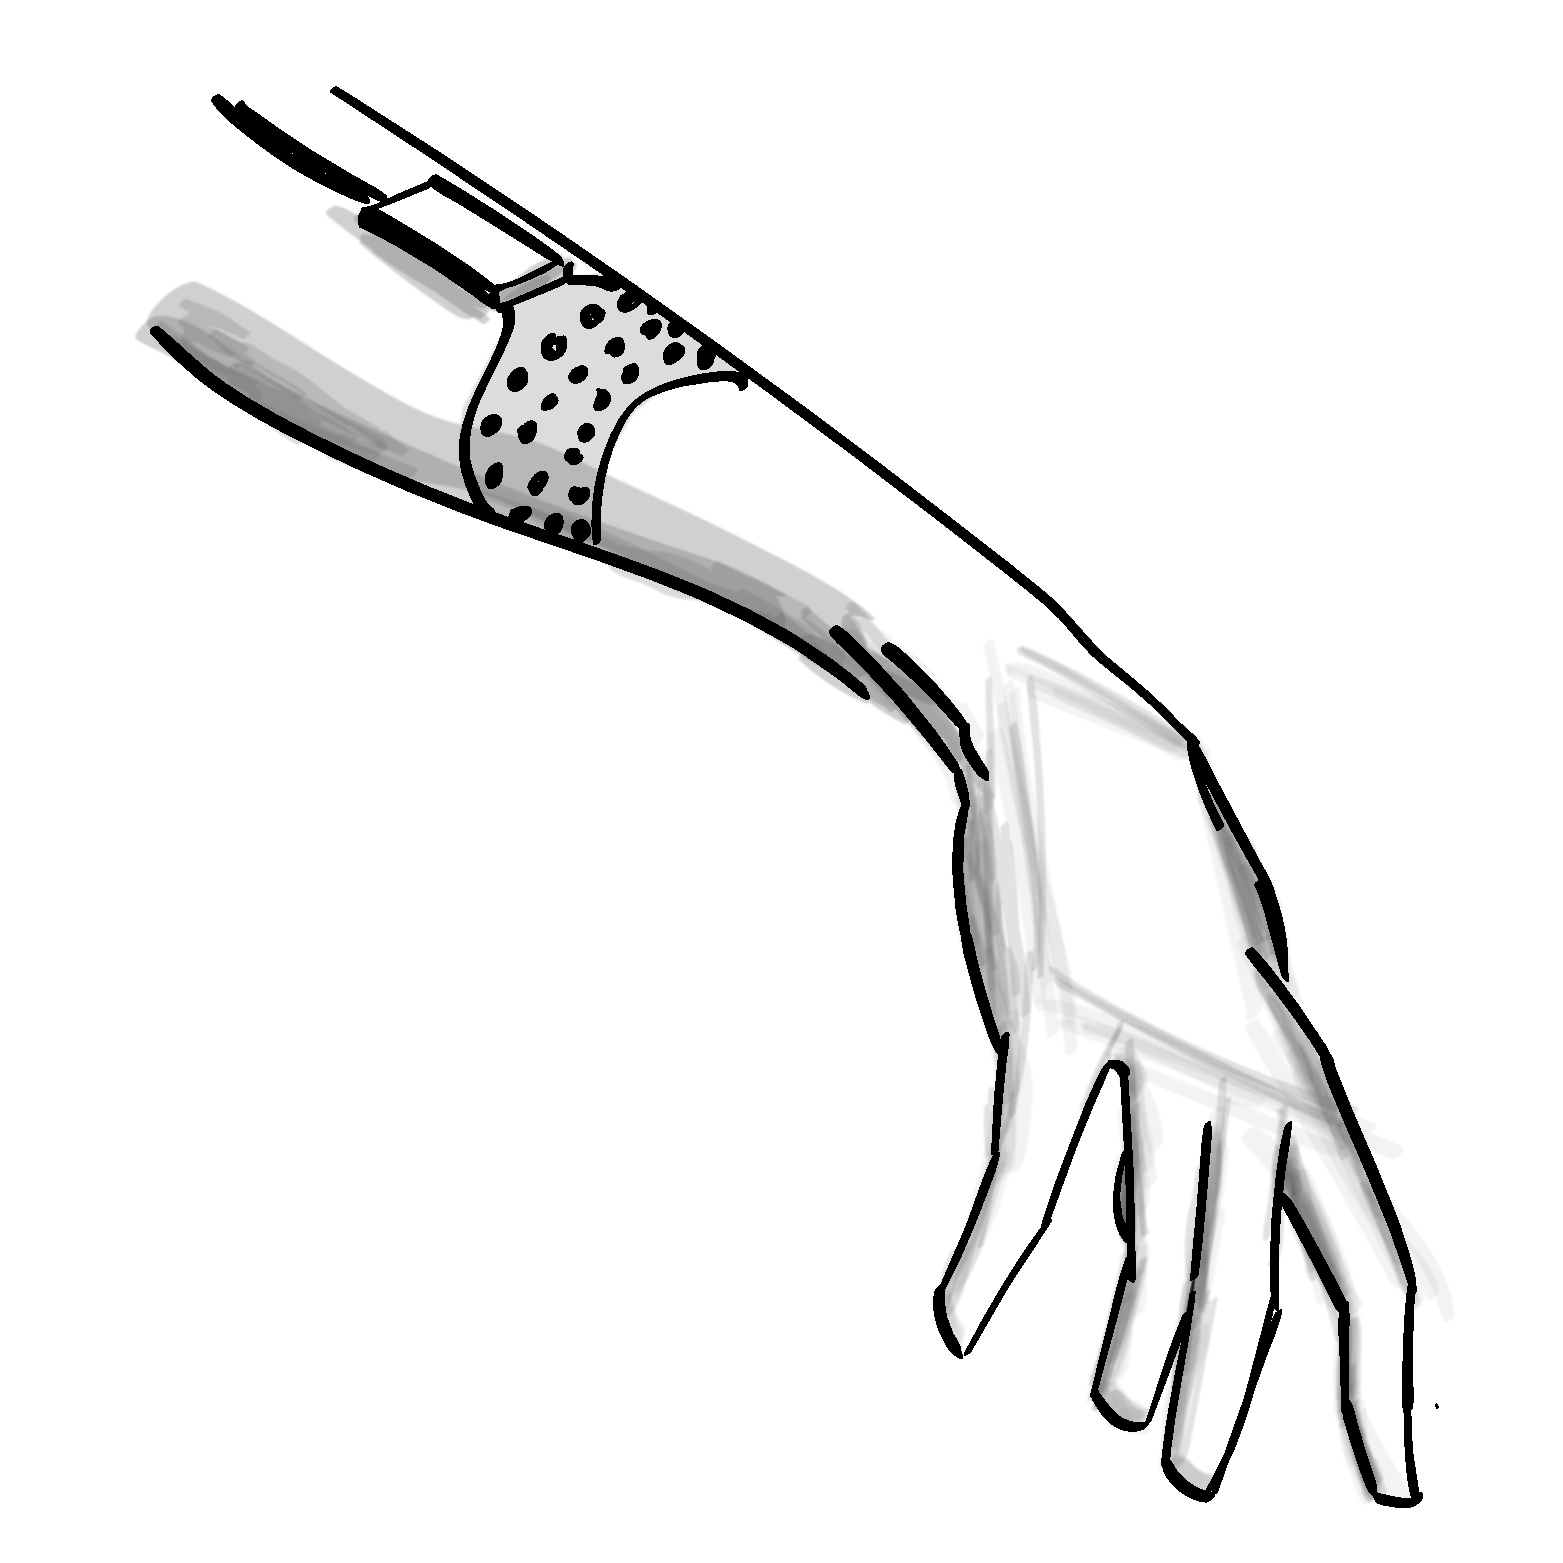
\includegraphics[page=1, width=\linewidth]{media/Ideasheet6.pdf}
            \subcaption{}\label{fig:IdeaSurfaceEMGBand}
        \end{minipage}
        \caption{Ideas}\label{fig:Idea}
    \end{figure}
    
    As can be understood from Section \emph{\ref{sec:IntroMotivation}}, I chose idea \ref{ItemDeltaChoice}\ref{ItemEMG} and, of it, naturally the least invasive variant of the methods, namely \emph{sEMG} \footnote{Surface Electromyography} because of the conditions of use, which can be classified as automotive grade\footcite[]{AutomotiveGrade:Wiki}\footnote{Meaning the reliability grade of components given by their characteristics such as resistance to high temperatures, vibrations and other physical impacts} and even extreme.
    The downsides of the choice are the weakness of the initial signal compared to the \emph{EMI} \footcite[Electromagnetic interference]{EMI:Wiki} of the environment, but this problem is easily solvable with a smart sensor design.
    
    \subsection{Introduction to the theory}\label{sec:IntroFiltersSignals}
    A signal serves to transmit information; the interference caused by other sources\footnote{Intentional or not} of signals of the same type can alter the information encoded in it.
    In some cases it is possible to prevent interference, in others this turns out to be impossible or ineffective.
    Reading the EMG signal falls into the second category of cases.
    In such situations filters are used\footnote{In Section \ref{sec:SensorboardDesignInput} it will become clear that this is a frequency filter}.
    
    A filter, in signal processing terms, is a device or process that is able to remove some components from the supplied signal \footcite[]{Filter:Wiki}.
    From a theoretical point of view, different types of filters can be described in mathematical language, namely with their transfer function\footnote{Moreover, not every function can be implemented; this will be clarified in Section \ref{sec:MathAndPhysics}}.
    Without lengthening the concrete discussion in this Section, it should be understood that, in order to work, the abstraction must be implemented in the real world using some of its properties and phenomena: as chosen previously, I will use electricity to represent the initial model.

    Before starting to understand how filter implementations work, one must understand how information is represented using the phenomenon of electricity.
    Technology, in the field of electronics, has two methods used everywhere to represent information: in digital form and in analog form.
    \begin{figure}[H]
        \centering
        \begin{tikzpicture}
            \begin{axis}[
                axis x line=bottom,
                axis y line=middle,
                xlabel={$t[ms]$},
                ylabel={$U[{\mu}V]$},
                legend entries={$(a)$, $(b)$},
                legend pos=north east,
                height=.4\textwidth,
                width=.75\textwidth,
                clip=true,
                xtick distance=200,
                ytick distance=200,
                xmin=600,
                xmax=1600,
                ymin=-400,
                ymax=500,
                smooth,
                ymajorgrids=true,
                grid style=dashed,
                axis_style_default
            ]
                \addplot[
                    color=darkgray!75,
                    thick
                    ]
                    table {datasets/ecg_example_data/ecg_example_data};
                \addplot[
                    only marks,
                    color=red!75,
                    mark size=.275ex,
                    thick,
                    every mark/.append style={solid, fill=red!75, mark=*},
                    ]
                    table {datasets/ecg_example_data/ecg_bin_example_data};
            \end{axis}
        \end{tikzpicture}
        \caption{The plot shows two human ECG \emph{(Electrocardiogram)} signals, read by a single EMG \emph{(Electromyographic)} sensor, with the signal analog in $(a)$ and after it has been digitized in $(b)$ \parenciteit{}{ECGDataThesis}\parenciteit{}{ECGData}}
        \label{fig:AnalogDigital}
    \end{figure}

    As can be seen in Figure \ref{fig:AnalogDigital}, the analog signal can be attributed the characteristic of a continuous course: the function contains an infinity of data points in a non-zero time interval.
    The digital signal, instead, presents us periodically with a single point: the signal is composed of a limited number\footnote{It can also be zero if the chosen time span is shorter than the sampling period} of data points in a non-zero time interval.
    Moreover, we know that the digital signal is related to the analog one through \emph{digitization}, also called \emph{discretization}\footcite["Process of transferring continuous functions, models, variables, and equations into discrete counterparts"]{Discretization:Wiki} when it is more of a mathematical context.
    The difference between the two methods of representing information will be discussed in more depth in Section \ref{sec:ProjectDesign}.
    The division into signal types naturally also concerns the parts that transform it, for example filters.

    At this point the knowledge of the topic is sufficient to follow the discussion that comes next.

    \section{Project characteristics}\label{sec:ProjectCharacteristics}
    Very often it is difficult to make choices during the design process.
    To reduce the time spent, it is good practice to start by trying to define the most important characteristics of the project, order them, make them concrete and quantify them as much as possible, then selecting only those that are most relevant among the others.
    One must not forget that the procedure, even if carried out consistently, can still lead to sequences of choices that will result in an impossible or impractical project, or altogether in a situation describable as: "\emph{Not what was wanted}".
    The solution is to constantly modify the required characteristics and the design as soon as a deviation is noticed.
    Instead of proceeding to realize the ideas by sticking to choices based on initial theoretical models and practical experience that one does not want to admit are false, inadequate or outdated, it is better to focus on what reality dictates in this regard.

    \begin{figure}[H]
        \Centering
        \vspace{1ex}
        \textit{"Theory and practice sometimes clash. And when that happens, theory loses. Every single time."}

        \RaggedLeft
        \vspace{1ex}

        \textit{\scriptsize{Linus B. Torvalds}}
        \vspace{1ex}
    \end{figure}

    Considering the complexity of the project, I tend to choose a project management\footnote{Management of the project's activities} method that I partly link to software development approaches\footcite[]{SoftwareDevelopmentProcess:Wiki}.
    I believe it is more than possible to use\footnote{Of course with some modifications} software development approaches also for projects that are not confined to the field of computer science and that are not exclusively large-scale in terms of the people involved.
    \begin{figure}[H]
        \centering
        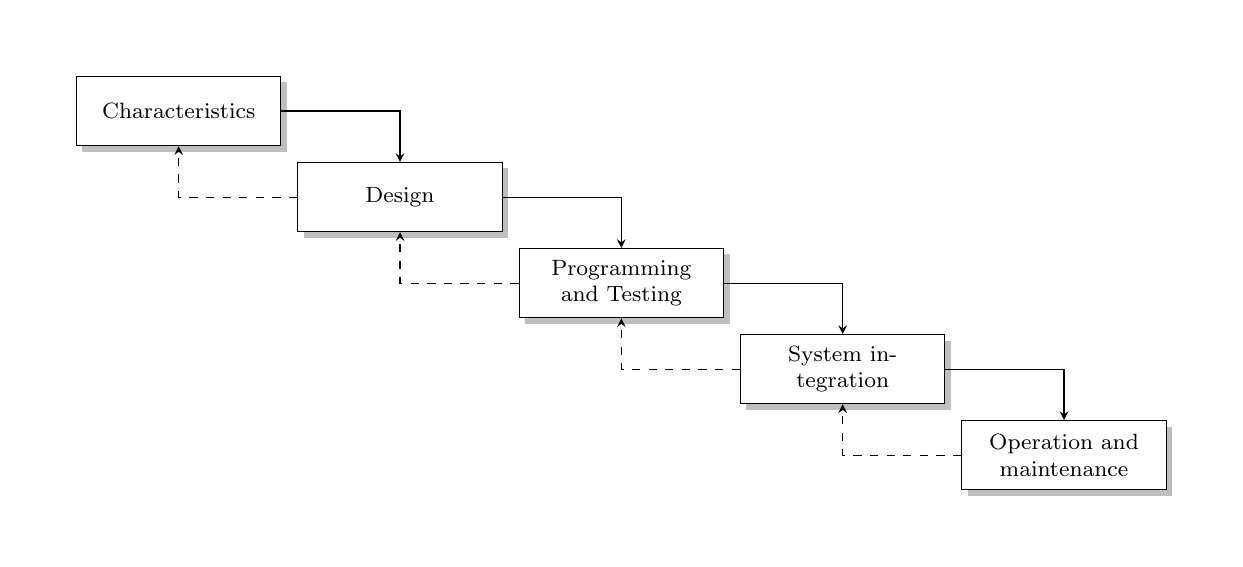
\begin{tikzpicture}[
            node distance = 2mm and 2mm,
            start chain = Waterfall going below right,
            every node/.style = {
                block,
                text width=16ex,
                minimum height=2.5em,
                inner sep=.25em,
                on chain=Waterfall,
                font_size
            },
        ]
            \node {Characteristics};
            \node {Design};
            \node {Programming and Testing};
            \node {System integration};
            \node {Operation and maintenance};
            \foreach \i [count=\j] in {2,...,5}{
                \draw[->, dashed] (Waterfall-\i) -| (Waterfall-\j);
                \draw[->] (Waterfall-\j) -| (Waterfall-\i);
            }
            \draw \InvisibleBorder;
        \end{tikzpicture}
        \caption{Waterfall software development approach}
        \label{fig:Waterfall}
    \end{figure}
    Over time the Waterfall model approach to software design\footcite[]{WaterfallModel:Wiki} \emph{(Figure \ref{fig:Waterfall})} proved utopian and ineffective for the real world, and was subsequently replaced by much newer, more effective and more dynamic approaches such as Agile\footcite[]{AgileModel:Wiki}, Scrum\footcite[]{ScrumModel:Wiki} and DevOps\footcite[]{DevOpsModel:Wiki}.
    The advice to be dynamic in the "\emph{Requirements}"\footnote{That is, characteristics, objectives} and the "\emph{Design}"\footnote{Choices and motivations of the "\emph{Requirements}"} and to try to change the characteristics of the project to adapt it to the influence of the concrete world is precisely the philosophy behind the recent approaches that I try to apply to my working method.

    \noindent The main characteristics of the project:
    \begin{enumerate}[label=\emph{(\arabic*)}]
        \item To be able to do what it was conceived for: \emph{read, transform and transmit the signal reliably} \label{char:Reliability}
        \item To try to \emph{not hinder the movement} of the hand and arm because of its \emph{size} and \emph{weight} \label{char:CompactNoDriveImpact}
        \item To be \emph{compact} enough to fit under a jacket \label{char:Compact}
        \item To have some degree of \emph{repairability} without compromising characteristic \ref{char:Compact} too much \label{char:Repairability}
        \item To be \emph{comfortable} to use, not scratch the hand, not distract the person \label{char:ComfortableNoPain}
        \item To have an \emph{operating} time of more than 5 hours \label{char:Automaticity}
        \item To provide \emph{intuitive control} of the vehicle \label{char:IntuitiveControl}
        \item Not to be an obstacle in \emph{stressful} situations \label{char:StressReactionAdapted}
        \item To be \emph{resistant to external factors} such as impacts, water, absence of airflow \label{char:ExternalImpactAdapted}
        \item To be able to configure the gestures needed \label{char:GestureVariability}
    \end{enumerate}
    \todo{check references in the document to the points above}
    Some points may seem unrelated to the design of a small part such as the sensor, but the reason behind them is that the list is not the result of linear development, but of iterating the dynamic design approach, and every point listed above has an influence on the design\footnote{Some points will be mentioned with a reference in the more concrete sections such as \ref{sec:ProjectDesignAbstractModel} or \ref{sec:MotherboardDesign}}. \todo{correct after previous fix}

    \section{Project design}\label{sec:ProjectDesign}
    The modus operandi\footnote{Tactic, habitual way of acting} applied in this Section is that of abstraction: it consists of simplifying the initial idea into a generic model and then gradually making it concrete.

    \subsection{Abstract model}\label{sec:ProjectDesignAbstractModel}
    The remote control can conveniently be represented with a block diagram\footcite[]{BlockDiagram:Wiki} \emph{(Figure \ref{fig:BlockDiagram})} in order to understand which system architecture\footnote{Meaning the implementation model} and implementation to choose.
    \begin{figure}[H]
        \centering
        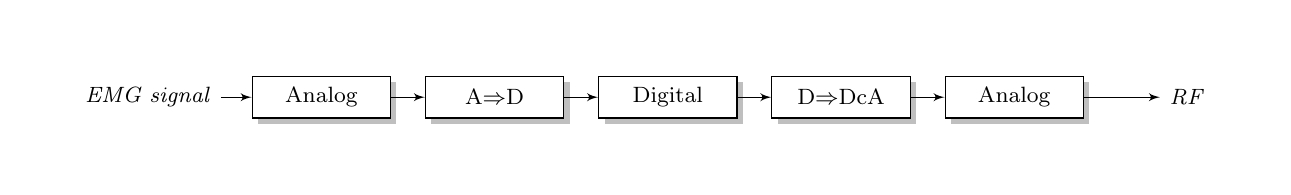
\begin{tikzpicture}[auto,>=latex', font_size, box_width/.style={minimum width=5em}]
            \draw (0,0)
                node at (0,0) (input) {\textit{EMG signal}};
            \draw (input)
                node[box_width, block] at ++(2.2,0) (block_analogue1) {Analog};
            \draw[->] (input.east) -- (block_analogue1.west);
            \draw (block_analogue1)
                node[box_width, block] at ++(2.2,0) (block_intermediate1) {A$\Rightarrow$D}
                [->] (block_analogue1.east) -- (block_intermediate1.west);
            \draw (block_intermediate1)
                node[box_width, block] at ++(2.2,0) (block_digital) {Digital}
                [->] (block_intermediate1.east) -- (block_digital.west);
            \draw (block_digital)
                node[box_width, block] at ++(2.2,0) (block_intermediate2) {D$\Rightarrow$DcA}
                [->] (block_digital.east) -- (block_intermediate2.west);
            \draw (block_intermediate2)
                node[box_width, block] at ++(2.2,0) (block_analogue2) {Analog}
                [->] (block_intermediate2.east) -- (block_analogue2.west);
            \draw (block_analogue2)
                node at ++(2.2,0) (output) {\textit{RF}}
                [->] (block_analogue2.east) -- (output.west);
            \draw \InvisibleBorder;
        \end{tikzpicture}
        \caption{}
        \label{fig:BlockDiagram}
    \end{figure}
    As can be seen, the \emph{Input} is the EMG signal, and to reach the RF communication channel, which corresponds to the \emph{Output}, the signal has to go through some modifications.
    % TRANSLATOR NOTE: kept the abbreviation "DcA" (Italian "Digitale codificato in Analogico") everywhere, incl. the block diagrams, and glossed it in the footnote; rename to e.g. "DeA" if you prefer an English acronym.
    The chain of transformations contains the "\emph{Analog}" block, which is meant to represent a part that transforms the signal continuously, the "\emph{A$\Rightarrow$D}" block, which digitizes the signal, the "\emph{Digital}" block, which transforms the information discretely, and the "\emph{D$\Rightarrow$DcA}"\footnote{"DcA" stands for the Italian \emph{Digitale codificato in Analogico}, i.e. digital encoded as analog} block, which encodes digital information into another form\footnote{Through a signal technique called "\emph{Modulation}" \parencite[]{Modulation:Wiki}} that can be transmitted via RF.

    \noindent The question arises as to why not eliminate the "\emph{A$\Rightarrow$D}", "\emph{Digital}" and "\emph{D$\Rightarrow$DcA}" blocks and replace the whole scheme with a single "\emph{Analog}" block\footnote{It represents a transformation of the analog signal into RF without digitization and without any modulation (also changing the way information is transmitted, without the modulation method due to the absence of the signal in digital form)}.

    \nopagebreak
    \noindent Reasons:
    \begin{enumerate}[label=\emph{(\arabic*)}]
        \item Current impracticality.
        Many computations tend to be done on digital devices, and consequently analog solutions with similar cost and computing power cannot be found on the market.
        \item The second reason is the precision and the resistance of the system to external factors.
        A signal represented in analog form contains infinitely more information\footnote{The difference can be seen in Section \ref{sec:IntroFiltersSignals}} \footnote{For signals converted from the digital to the analog representation, the missing information is filled in} compared with its digitized form, and can easily be altered during processing or transmission.
        To represent a digital signal, normally, the binary system is used: it is much less likely to alter a signal that uses, for example, half of its amplitude for a "1" and the other half for a "0" than a value encoded in an infinitesimal fraction of its amplitude.
        Moreover, electronic components are used to modify a signal\footnote{This will be explored in Section \ref{sec:MathAndPhysics}}, and in the real world they have imperfections that can be represented as additional elements called parasitics \emph(Figure \ref{fig:ExampleParassiticElements}) and, because of the nature of the analog signal, they affect the information much more and in unforeseen ways\footnote{The digital signal is also altered during processing, but the consequences can be remedied with circuits such as Schmitt triggers\parenciteit{}{SchmittTrigger:Wiki}, whereas for the analog signal this is not applicable}.
        The same applies to RF transmission: the signal without modulation, i.e. not digitized, will be less resistant to EMI.
        \item The third reason is that not all functions can be implemented: for example, it is impossible to implement non-deterministic functions as a network of analog components\footnote{While keeping the circuit operating in analog form}, and difficult or impossible for functions that describe TV systems\footnote{Time-variant, i.e. varying over time}\:\footcite[]{TimeVariantSystem:Wiki}.
    \end{enumerate}

    \begin{figure}[H]
        \centering
        \begin{minipage}[H]{.4\linewidth}
            \centering
            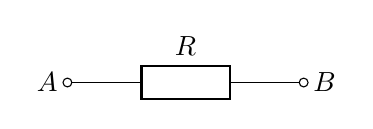
\begin{tikzpicture}[transform shape, use fpu reciprocal]
                \draw (0,0)
                    node[left]{$A$}
                    to[short, o-] ++(.5,0)
                    to[R, l=$R$] ++(2,0)
                    to[short, -o] ++(.5,0)
                    node[right]{$B$};
            \end{tikzpicture}
            \subcaption{Simple representation of a resistor of value $R$}
            \label{fig:ExampleParassiticElementsSimple}
        \end{minipage}
        \hspace*{0.04\linewidth}
        \begin{minipage}[H]{.4\linewidth}
            \centering
            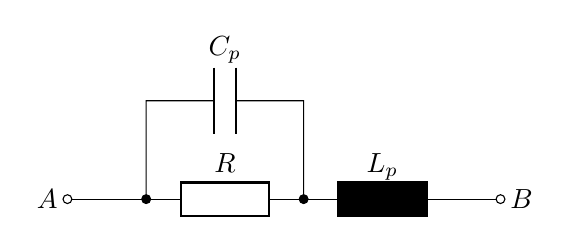
\begin{tikzpicture}[transform shape, use fpu reciprocal]
                \draw (0,0)
                    node[left]{$A$}
                    to[short, o-] ++(1,0)
                    coordinate(AR)
                    to[R, l=$R$, -*] ++(2,0)
                    coordinate(RL)
                    to[L, l=$L_p$] ++(2,0)
                    to[short, -o] ++(.5,0)
                    node[right]{$B$};
                \draw (AR)
                    to[short, *-] ++(0,1.25)
                    to[C, l=$C_p$] ++(2,0)
                    -- (RL);
            \end{tikzpicture}
            \subcaption{More refined representation of a resistor of value $R$, which can be affected by $C_p$ and $L_p$, the parasitic capacitance and inductance}
            \label{fig:ExampleParassiticElementsRefined}
        \end{minipage}
        \caption{Example of two models of a resistor}
        \label{fig:ExampleParassiticElements}
    \end{figure}

    \noindent A second question arises as to why not eliminate the two "\emph{Analog}" blocks.

    \nopagebreak
    \noindent Reasons:
    \begin{enumerate}[label=\emph{(\arabic*)}]
        \item The "\emph{A$\Rightarrow$D}" block requires, and the "\emph{D$\Rightarrow$DcA}" block emits, a signal confined within precise voltage limits: for this reason it is necessary to adapt the signal voltage before letting it proceed.
        \item The signal is always contaminated by noise, and if it is digitized without analog filtering it risks corrupting the data\footnote{This can lead to a system malfunction if the data are processed directly, or to a reduced amount of information if digital filter implementations are used}.
        \item An analog filter implementation costs less than a digital one of the same effectiveness.
        \item The amount of data collected and processed discretely is directly linked to computing power and speed: as the amount of processed data increases, the digital filter needs more computing power to work, whereas the analog filter will not be affected in any way. \label{reas:SamplingRateVsDigitalAnalogFilters}
        \item Referring to point \ref{reas:SamplingRateVsDigitalAnalogFilters}, an analog filter implementation in most cases\footnote{It depends on the acquisition rate of the discrete data} consumes less energy\footnote{This will become clear in Section \ref{sec:ProjectDesignAbstractModel}} than a digital one of the same effectiveness.
        \item When digitizing an unfiltered signal there is a greater risk of clipping\footnote{Exceeding the predefined voltage limits of the circuit responsible for digitization, which normally leads to the loss of part of the data} \footnote{It can be prevented by increasing the maximum and minimum limits of the circuit responsible for digitization, but then the resolution of the signal starts to decrease; if one wants to maintain it, a different, more expensive digitizing circuit must be chosen} of the signal.
    \end{enumerate}

    \subsection{Implementation model}\label{sec:ProjectDesignImplementationModel}
    The implementation model is the most concrete model possible without having chosen the concrete components of the implementation; it can help to understand all the possibilities right before choosing them.

    The number of EMG signals depends on the muscles from which one wishes to detect information.
    This information is dictated by the gestures\footnote{The system must be flexible so that the desired gestures can be configured} that one wants to read; for this reason\footnote{Reference to project characteristic "\ref{char:GestureVariability}" in Section \ref{sec:ProjectCharacteristics}} the number of electrodes, the conceptual part closest to signal acquisition, must be variable.
    Transmitting the signal as it is picked up by the electrodes is a bad idea because of the weakness of the signal compared to the environmental EMI.
    Consequently the signal must be amplified before being transmitted, but the loss of information in the analog signal still remains.
    To make the precision of the information less sensitive to EMI, it is good practice to digitize the signal before transmitting it.
    The decision just described increases the cost of the device because of the price of standalone ADCs\footnote{Analog to digital converter}, which moreover must be many single-channel ones\footnote{This reduces the possibility of using types of ADC with MUXes \parenciteit{}{Multiplexer:Wiki}, which allow the part implementing the digitizing circuit, the most expensive part of the integrated circuit, to be reused across several channels}, but the reliability of the circuit is more important to me\footnote{Reference to project characteristic "\ref{char:Reliability}" in Section \ref{sec:ProjectCharacteristics}}.

    The digital part, unlike the analog and the digitizing parts, does not need to be decentralized, also because of the tendency towards higher cost\footnote{In our case these are complex parts containing memory, a processor and other components, which would have to be duplicated for every additional chip used (thereby increasing the cost)} of chips when several are used instead of one, and because of the higher communication latencies\footnote{If one wants to avoid them, more specialized chips must be chosen, again increasing the cost}.

    For the modulator and the RF signal amplifier, existing chips that implement both functions together can be used: this reduces costs while decreasing flexibility in the choice of communication protocols that can be used and in the range of the device.
    The choice is entirely possible and logical given the small need to support many protocols or to operate over a varied range of distances.
    Moreover, the chip responsible for modulation can sometimes be found implemented directly in the circuits we see in the digital part category\footnote{SoC \parenciteit{}{SoC:Wiki}, microcontrollers}.
    The decision to merge the modulator, the signal amplifier and the digital part can reduce latency and increase the data transmission speed of the system thanks to the parallel interface frequently used inside the chips' silicon, which is also cheaper compared to interfaces between different pieces of silicon that leave the chip\footnote{The most common are $I_2 C$ \parenciteit{}{I2C:Wiki} and $SPI$ \parenciteit{}{SPI:Wiki}}, but this question will be made concrete later in Section \ref{sec:MotherboardDesignInterface}.

    \noindent At the end of the reasoning we obtain two schemes, as shown in Figure \ref{fig:ConcretizedBlockDiagram}
    \nopagebreak
    \begin{figure}[H]
        \centering
        \begin{minipage}[H]{\linewidth}
            \centering
            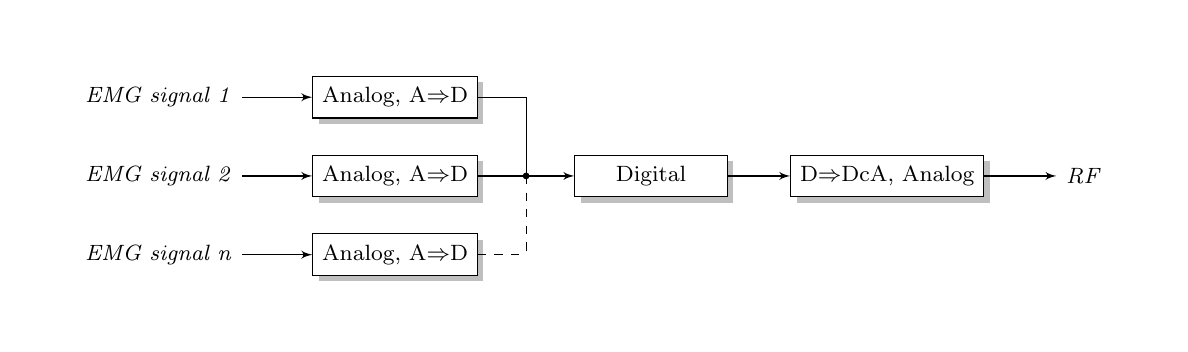
\begin{tikzpicture}[auto,>=latex', font_size, box_width/.style={minimum width=5.5em}]
                \foreach \n in {1,2}{
                    \node at (0,-\n+2) (input\n) {\textit{EMG signal \n}};
                };
                \node at (0,-3+2) (input3) {\textit{EMG signal n}};
                \foreach \n in {1,2,3}{
                    % \node at (0,-\n+2) (input\n) {\textit{Segnale EMG\n}};
                    \node[box_width, block] at ++(3,-\n+2) (block_analogue1_\n) {Analog, A$\Rightarrow$D};
                    \draw[->] (input\n.east) -- (block_analogue1_\n.west);
                };
                \draw (block_analogue1_2)
                    node[box_width, block] at ++(3.25,0) (block_digital) {Digital};
                \foreach \n in {1,2}{
                    \draw ($(block_analogue1_\n.east)!.5!(block_digital.west)$)
                        coordinate(iter_arrow_\n)
                        [-] (block_analogue1_\n.east) -- (iter_arrow_\n |- block_analogue1_\n.east)
                        coordinate(iter_arrow_end_\n);
                };
                \draw ($(block_analogue1_3.east)!.5!(block_digital.west)$)
                        coordinate(iter_arrow_3)
                        [dashed] (block_analogue1_3.east) -- (iter_arrow_3 |- block_analogue1_3.east)
                        coordinate(iter_arrow_end_3);
                \draw[-] (iter_arrow_end_1) -- (iter_arrow_end_2);
                \draw[dashed] (iter_arrow_end_2) -- (iter_arrow_end_3);
                \draw[->] (iter_arrow_end_2) -- (block_digital.west);
                \filldraw (iter_arrow_end_2) circle (1pt);
                \draw (block_digital)
                    node[box_width, block] at ++(3,0) (block_intermediate2) {D$\Rightarrow$DcA, Analog}
                    [->] (block_digital.east) -- (block_intermediate2.west);
                \draw (block_intermediate2)
                    node at ++(2.5,0) (output) {\textit{RF}}
                    [->] (block_intermediate2.east) -- (output.west);
                \draw \InvisibleBorder;
            \end{tikzpicture}
            \subcaption{Model with the modulator and signal amplifier separate from the digital part}
            \label{fig:ConcretizedBlockDiagramMulti}
        \end{minipage}
        \begin{minipage}[H]{\linewidth}
            \centering
            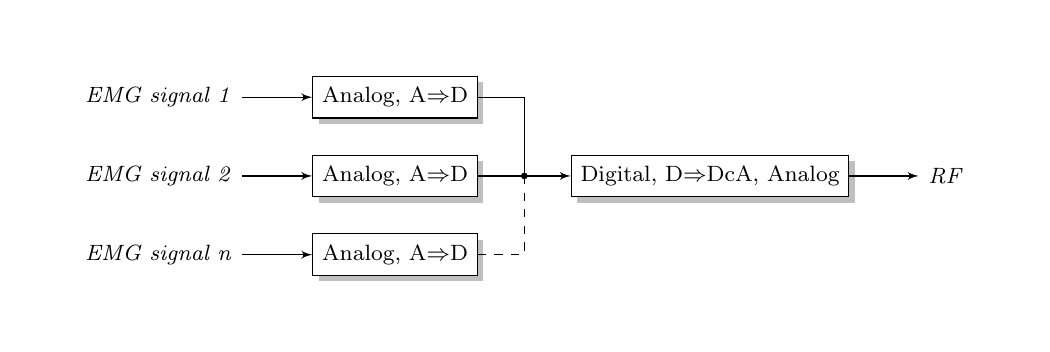
\begin{tikzpicture}[auto,>=latex', font_size, box_width/.style={minimum width=5.5em}]
                \foreach \n in {1,2}{
                    \node at (0,-\n+2) (input\n) {\textit{EMG signal \n}};
                };
                \node at (0,-3+2) (input3) {\textit{EMG signal n}};
                \foreach \n in {1,2,3}{
                    % \node at (0,-\n+2) (input\n) {\textit{Segnale EMG\n}};
                    \node[box_width, block] at ++(3,-\n+2) (block_analogue1_\n) {Analog, A$\Rightarrow$D};
                    \draw[->] (input\n.east) -- (block_analogue1_\n.west);
                };
                \draw (block_analogue1_2)
                    node[box_width, block] at ++(4,0) (block_digital) {Digital, D$\Rightarrow$DcA, Analog};
                \foreach \n in {1,2}{
                    \draw ($(block_analogue1_\n.east)!.5!(block_digital.west)$)
                        coordinate(iter_arrow_\n)
                        [-] (block_analogue1_\n.east) -- (iter_arrow_\n |- block_analogue1_\n.east)
                        coordinate(iter_arrow_end_\n);
                };
                \draw ($(block_analogue1_3.east)!.5!(block_digital.west)$)
                        coordinate(iter_arrow_3)
                        [dashed] (block_analogue1_3.east) -- (iter_arrow_3 |- block_analogue1_3.east)
                        coordinate(iter_arrow_end_3);
                \draw[-] (iter_arrow_end_1) -- (iter_arrow_end_2);
                \draw[dashed] (iter_arrow_end_2) -- (iter_arrow_end_3);
                \draw[->] (iter_arrow_end_2) -- (block_digital.west);
                \filldraw (iter_arrow_end_2) circle (1pt);
                \draw (block_digital)
                    node at ++(3,0) (output) {\textit{RF}}
                    [->] (block_digital.east) -- (output.west);
                \draw \InvisibleBorder;
            \end{tikzpicture}
            \subcaption{Model with the modulator and signal amplifier merged with the digital part}
            \label{fig:ConcretizedBlockDiagramMono}
        \end{minipage}
        \caption{Abstract models of the project made as concrete as possible without a final choice of components}
        \label{fig:ConcretizedBlockDiagram}
    \end{figure}
    From now on, to indicate the conceptual union of blocks I will use the terms "sensor board" for the "\emph{Analog}", "\emph{A$\Rightarrow$D}" blocks and "main board"\footnote{It groups all the blocks that are single and do not need to be placed in a specific location} for the "\emph{Digital}", "\emph{D$\Rightarrow$Dca}", "\emph{Analog}" blocks: the separation of the two concepts is given by the interface from the "\emph{A$\Rightarrow$D}" block to the "\emph{Digital}" block.

    \subsection{Organization of the following parts}
    In our case it is easier to start making the implementations concrete by beginning with the main board\footnote{Clarified at the end of Section \ref{sec:ProjectDesignImplementationModel}}, which is single, can group several blocks and is less flexible than the sensor board\footnote{Clarified at the end of Section \ref{sec:ProjectDesignImplementationModel}} in terms of choices.
    The design of the sensor board is done mainly at the level of SMD\footcite[]{SMT:Wiki} and TH\footcite[]{THT:Wiki} components, whereas the main board only allows us to choose existing solutions\footnote{To reduce size and costs I would opt not to add functionality beyond that offered by the main chip (and perhaps by the modulator)}.
    Moreover, although the main board is not part of the subject of the \emph{maturit\`{a}} thesis, it influences the choice of the digital protocol for transmitting the signal information from the sensor board to the main board, and it plays an indispensable role both in the final version of the sensor and in the prototype model: for this reason it must also be made concrete.

    \section{Main board}\label{sec:Motherboard}
    \begin{samepage}
        \subsection{Characteristics}\label{sec:MotherboardCharacteristics}
            The main board, the set of the "\emph{Digital}", "\emph{D$\Rightarrow$DcA}", "\emph{Analog}" blocks, must meet the following characteristics:
            \begin{enumerate}[label=\emph{(\arabic*)}]
                \item Consume little energy to process information (without harming latency and computing power)
                \item Consume little energy to encode and amplify the signal (without harming latency and computing power)
                \item Have a power-saving mode
                \item Have interfaces to communicate with many analog blocks (with digital interfaces provided by the ADCs\footnote{Part of the "\emph{A$\Rightarrow$D}" block that contains it})
            \end{enumerate}
    \end{samepage}

    \begin{samepage}
        \subsection{Design}\label{sec:MotherboardDesign}
        \noindent The things we can choose are:
        \begin{enumerate}[label=\emph{(\arabic*)}]
            \item The firmware\footnote{Meaning the program that handles low-level tasks} of the chip
            \item The program\footnote{Meaning the program that handles the main tasks of the chip} of the chip
            \item The "\emph{central}" chip\footnote{Whose function is to execute the algorithms given by the programs to allow the remote control to operate} (with or without integrated RF connection support)
            \item The RF connection support chip (if the option of a "\emph{central}" chip without these capabilities has been chosen)
            \item The power supply and battery management circuit
        \end{enumerate}
    \end{samepage}

    % TRANSLATOR NOTE: "automaticita" (here and in char:Automaticity) read as battery autonomy / operating time -> "autonomy time".
    The chip must consume little energy so as not to overheat\footnote{This issue is secondary because the problem can be solved with cooling solutions} and so as not to reduce the autonomy time\footnote{Reference to project characteristic \ref{char:Automaticity}} of the device, but at the same time energy consumption affects\footnote{Non-linearly, because of the various optimizations implemented in the chip's silicon, which depend on its ISA \parenciteit{}{ISA:Wiki}} computing power\footnote{Reference to project characteristic \ref{char:Reliability}}.

    \subsubsection{Software}\label{sec:MotherboardDesignSoftware}
    The choice of firmware and program depends on the complexity of the data processing, on the multitasking\footnote{Carrying out more than one activity at the same time} needs I must meet and on the hardware I intend to use.
    Primarily, to eliminate the factor introduced by the hardware, I make sure to choose something with enough computing power to cover the computing power needs of the program.
    The program can be either a bare-metal program, which is started by the firmware after all the chip's functions have been initialized, or an operating system that manages the chip's resources to balance their use and to allow convenient use of more complex protocols\footnote{Such as WiFi, Bluetooth, USB}.
    The ideal chip for this task would be a mid-range one with a fairly high processor clock frequency\footnote{In this way I try to reduce data transmission and processing latency}, because the only work it has to do is to read the signals from the ADCs and then encode them using RF protocols.

    Meanwhile, at the prototyping stage, it would be perfectly fine to use a program written with the help of PlatformIO\footnote{A platform for C/C++ code development with broad hardware and framework support (for example Arduino and Zephyr RTOS, discussed below), convenient also for developing large multi-file projects} and a simple framework such as Arduino, whereas later, at the main board development stage\footnote{Not part of the \emph{maturit\`{a}} thesis}, it would suffice to use an operating system (necessarily with the characteristic of being an RTOS\footcite[]{RTOS:Wiki} \footnote{The type of operating system characterized by the ability to reduce the latency of the start of command execution as much as possible} \footnote{It is applied in conditions where an activity is of critical importance \parenciteit{}{MissionCritical:Wiki}}) such as those offered by the $\mu$COS or Zephyr RTOS projects\todo{Add to the global characteristics}
    if one wants to add a visual interface for reading the system status and a physical one for detailed control\footnote{This entails a more complex program with more parallel algorithms, which is not always needed while using the vehicle and could consequently potentially be optimized by using an RTOS}.

    Obviously, when it comes to developing devices whose main characteristics are efficiency with minimal compromises on data processing and transmission latency, options involving a GPOS\footnote{General Purpose Operating System, for example Linux, MacOS, Windows} and high-level programming languages\footnote{They are normally interpreted rather than compiled, which makes development easier but requires more powerful hardware to achieve results similar to low- or mid-level languages such as C or C++}\:\footnote{For example: Python, Java, C\#, JavaScript} are discarded immediately.
    
    % TRANSLATOR NOTE: this \todo is about Italian grammar ("dell'hardware" vs "del hardware") and is meaningless for the English text; kept as-is, safe to delete.
    \todo {"dell'hardware" instead of "del hardware"}
    
    It is also worth naming the programs I could use to visualize the data collected by the sensor on different devices\footnote{To process and study the data conveniently, I use communication between the main board prototype and the computer to export the data at the moment of collection}, for the sake of convenience in development and presentation\footnote{Currently, in 2021, Windows operating systems are much more widespread than Linux-based ones such as Debian, which I currently use to develop and document this project: consequently I must be able to present and run the project on platforms less familiar to me as well} of the project and flexibility during development: for me these would be Processing 4\footnote{A cross-platform program for developing code in a Java-based language} and the serial plotter of the Arduino IDE\footnote{A cross-platform program for developing code in a C/C++-based language}.

    \subsubsection{Interface}\label{sec:MotherboardDesignInterface}
    The only characteristic of the prototype that is not intended to change in the final model is the communication protocol between the main board and the sensor board.
    The options are rather few because of the simplicity of the system's implementation model\footnote{Section \ref{sec:ProjectDesignImplementationModel}}: it makes no sense to choose protocols such as UART or CAN\footnote{Even though in this specific case signal integrity, which is not supported in the other protocols, could be useful} since there is no second Master to communicate with.
    Consequently, the use of less sophisticated protocols is favored.

    % TRANSLATOR NOTE: original says "prevenire la calibrazione automatica" (literally "prevent"); context implies "prevedere" (provide for), translated as "enable automatic calibration".
    Deducing the characteristics of the protocol from the main project characteristics\footnote{Section \ref{sec:ProjectCharacteristics}} \ref{char:Repairability}, \ref{char:Reliability} and a limited budget, it is clear that: in view of the architecture\footnote{The implementation model of the remote control in Section \ref{sec:ProjectDesignImplementationModel} foresees the use of several sensor boards} of the sensor board, one of the most widespread interfaces is required\footnote{Relevant because of broad hardware implementation, software support and greater freedom in choosing the ADC}, with fairly low latency in bidirectional data communication\footnote{Bidirectional latency matters for communicating the amount of amplification and for data transmission, which could potentially be added in one of the next versions of the prototype to enable automatic calibration of the remote control (with reference to project characteristic \ref{char:IntuitiveControl})} so as to allow the rider of the vehicle to react quickly, and possibly simplicity of connection\footnote{The modular sensor system should not create confusion during connection and should reduce the possibility of malfunction during use, as could happen with parallel interfaces}.

    \vspace{2ex}
    \Centering
    The choice is between \emph{SPI} and \emph{I2C}.

    \vspace{2ex}
    \justifying

    Because of its way of communicating, I2C is known to introduce more latency\footnote{In the I2C protocol, besides the lower maximum possible communication frequency compared to SPI, the master must first communicate the Slave's address and only then start transmitting data, whereas SPI uses a pin that allows almost instantaneous access} in signal communication than SPI, while also having the advantage of always keeping the same\footnote{Information is always transmitted via SDA (the conductor that carries data) and SCL (the conductor that sets the pace of the transmission)} number of conductors for data transmission.
    For SPI, moreover, there are 4 conductors for transmitting information\footnote{MOSI, Master Out Slave In, MISO, Master In Slave Out, SCLK, Serial Clock, CS/SS, Chip/Slave Select}, and one of them, CS/SS, must be dedicated\footnote{To enable or disable communication between the Slave and the Master, the Master must change the state of the CS/SS output} to each individual chip one wants to communicate with.
    A better explanation is given in Figure \ref{fig:ExampleSPII2C}.
    The number of Slaves connected to the two interfaces is limited, in the case of SPI, by the number of pins\footnote{Conductive legs of the chip, which allow it to communicate with the things they are connected to} of the Master that can output voltages\footnote{Perform the Output function}, and in the case of I2C by the number of physical addresses frequently\footnote{Sometimes the address can be chosen with Slave pins reserved for that, and this is considered an extra option} implemented at the silicon level of the Slave, which is decided\footnote{There are services where chips can be ordered with any desired address, but this, again, is considered an extra option} by the chip manufacturer.
    \todo{Add example image on the differences between SPI and I2C communication}
    \begin{figure}[H]
        \centering
        \begin{minipage}[H]{\linewidth}
            \centering
            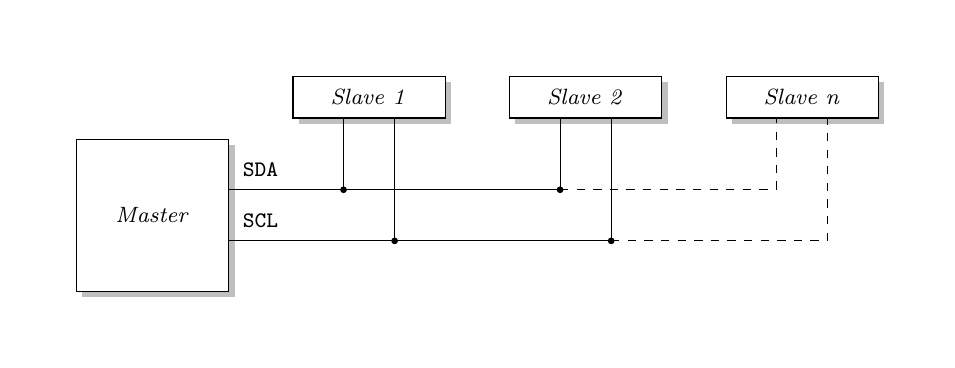
\begin{tikzpicture}[auto,>=latex', font_size, box_width/.style={minimum width=5.5em}]
                \node [box_width, block, minimum height=5.5em] at (0,0) (Master) {\textit{Master}};
                \foreach \n [evaluate=\n as \x using (\n/(2+1))] in {1,2}{
                    \draw ($(Master.north)!\x!(Master.south)$)
                        coordinate(Master_mid\n);
                    \draw (Master.east |- Master_mid\n)
                        coordinate(Master\n);
                };
                \foreach \i in {1,2}{
                    \node [box_width, block] at (\i*2.75,1.5) (Slave_\i) {\textit{Slave \i}};
                };
                \node [box_width, block] at (3*2.75,1.5) (Slave_3) {\textit{Slave n}};
                \foreach \i in {1,2,3}{
                    \foreach \n [evaluate=\n as \x using (\n/(2+1))] in {1,2}{
                        \draw ($(Slave_\i.west)!\x!(Slave_\i.east)$)
                            coordinate(Slave_\i_mid\n);
                        \draw (Slave_\i.south -| Slave_\i_mid\n)
                            coordinate(Slave_\i\n);
                    };
                };
                \foreach \n in {1,2}{
                    \draw [-] (Master\n) -- (Master\n -| Slave_2\n);
                    \foreach \i in {1,2}{
                        \filldraw (Master\n -| Slave_\i\n) circle (1pt);
                        \draw [-] (Master\n -| Slave_\i\n) -- (Slave_\i\n);
                    };
                    \draw
                        [dashed] (Master\n -| Slave_2\n) -- (Master\n -| Slave_3\n)
                        [dashed] (Master\n -| Slave_3\n) -- (Slave_3\n);
                };
                \foreach \masteri / \name / \intname in {1/SDA/sda, 2/SCL/scl}{
                        \node [anchor=south west] at ($(Master\masteri)+(0.05,0.05)$) (\intname) {\texttt{\name}};
                };
                \draw \InvisibleBorder;
            \end{tikzpicture}
            \subcaption{I2C protocol}
            \label{fig:ExampleI2C}
        \end{minipage}
        \begin{minipage}[H]{\linewidth}
            \centering
            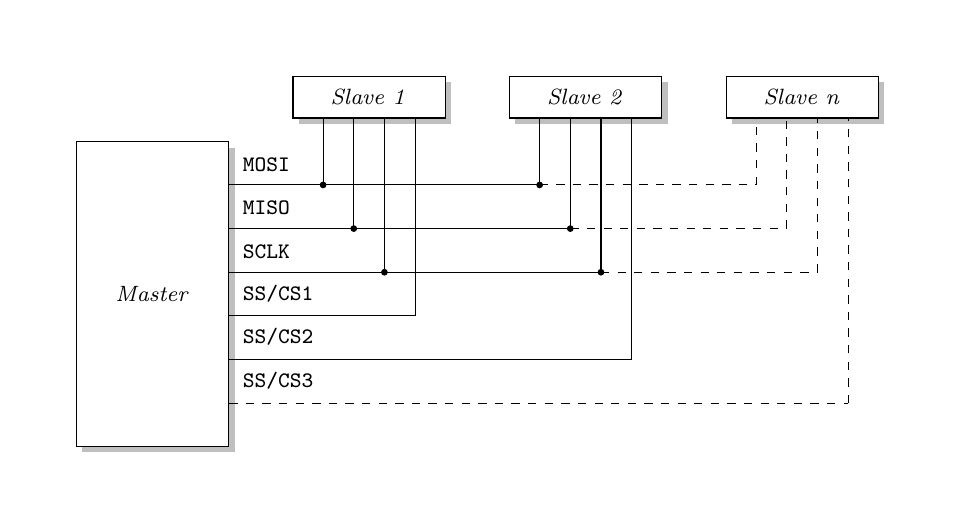
\begin{tikzpicture}[auto,>=latex', font_size, box_width/.style={minimum width=5.5em}, baseline={(current bounding box.center)}]
                \node [box_width, block, minimum height=11em] at (0,0) (Master) {\textit{Master}};
                \foreach \n [evaluate=\n as \x using (\n/(6+1))] in {1,2,...,6}{
                    \draw ($(Master.north)!\x!(Master.south)$)
                        coordinate(Master_mid\n);
                    \draw (Master.east |- Master_mid\n)
                        coordinate(Master\n);
                };
                \foreach \i in {1,2}{
                    \node [box_width, block] at (\i*2.75,2.5) (Slave_\i) {\textit{Slave \i}};
                };
                \node [box_width, block] at (3*2.75,2.5) (Slave_3) {\textit{Slave n}};
                \foreach \i in {1,2,3}{
                    \foreach \n [evaluate=\n as \x using (\n/(4+1))] in {1,2,...,4}{
                        \draw ($(Slave_\i.west)!\x!(Slave_\i.east)$)
                            coordinate(Slave_\i_mid\n);
                        \draw (Slave_\i.south -| Slave_\i_mid\n)
                            coordinate(Slave_\i\n);
                    };
                };
                \foreach \n in {1,2,3}{
                    \draw [-] (Master\n) -- (Master\n -| Slave_2\n);
                    \foreach \i in {1,2}{
                        \filldraw (Master\n -| Slave_\i\n) circle (1pt);
                        \draw [-] (Master\n -| Slave_\i\n) -- (Slave_\i\n);
                    };
                    \draw
                        [dashed] (Master\n -| Slave_2\n) -- (Master\n -| Slave_3\n)
                        [dashed] (Master\n -| Slave_3\n) -- (Slave_3\n);
                };
                \foreach \masteri / \slave in {4/1, 5/2}{
                    \draw
                        [-] (Master\masteri) -- (Master\masteri -| Slave_\slave4)
                        [-] (Master\masteri -| Slave_\slave4) -- (Slave_\slave4);
                };
                \draw
                        [dashed] (Master6) -- (Master6 -| Slave_34)
                        [dashed] (Master6 -| Slave_34) -- (Slave_34);
                \foreach \masteri / \name / \intname in {1/MOSI/mosi, 2/MISO/miso, 3/SCLK/sclk, 4/{SS/CS1}/sscs1, 5/{SS/CS2}/sscs2, 6/{SS/CS3}/sscs3}{
                        \node [anchor=south west] at ($(Master\masteri)+(0.05,0.05)$) (\intname) {\texttt{\name}};
                };
                \draw \InvisibleBorder;
            \end{tikzpicture}
            \subcaption{SPI protocol}
            \label{fig:ExampleSPI}
        \end{minipage}
        \caption{Block diagrams characterizing the communication between Master and Slave}
        \label{fig:ExampleSPII2C}
    \end{figure}
    \noindent Finally, the choice is dictated by the main project characteristic \ref{char:Repairability}, repairability, which with the choice of I2C becomes much more complex (the sensor boards stop being interchangeable), while the other main characteristic \ref{char:Compact} is not compromised: the conductors can be thin, flexible and easily hidden between two layers of fabric\footnote{The design characteristics of the project (meaning shape, materials) will be discussed in the next development stages, which are not part of the \emph{maturit\`{a}} thesis}. For this reason I decided to use the SPI protocol.

    \subsubsection{Hardware}\label{sec:MotherboardDesignHardware}
    The perfect choice would be the ESP32 product line\footnote{Precisely, the line of chips they are based on is meant} (an example is shown in Figure \ref{fig:ESP32_WROVER_B}), because of their qualitative characteristics (partially shown in Figure \ref{fig:ESP32_BD}), such as support for the WiFi, Bluetooth, BLE\footnote{Bluetooth Low Energy, not to be confused with "classic" Bluetooth (Bluetooth Basic Rate/Enhanced Data Rate, abbreviated BR/EDR) because the protocols differ in their characteristics and operation} \footcite[]{BLE:Wiki}, SPI, I2C\footnote{It could be useful for adding a screen in future versions of the prototype}, PWM and other protocols, the possibility of having more than one microprocessor\footnote{Meaning physical cores, which, depending on the architecture (in this case Xtensa LX6, which, unlike amd64 or ppc, has no SMT (Simultaneous Multithreading) capability \parenciteit{}{CPUSMT:Wiki}), have a number of logical cores equal to the number of physical cores} \footnote{In this way algorithms can be executed in parallel}, the power-saving mode\footnote{It works by lowering the clock frequency, the frequency that sets the pace of the processor}, and very low cost.
    As for the quantitative characteristics\footcite[]{ESP32:Datasheet}, such as the system frequency and the microcontroller voltage, they are also compatible with what is to be achieved:
    \begin{enumerate}[label=\emph{(\arabic*)}]
        \item The maximum frequency of the microcontroller: $190MHz$ - $240MHz$\footcite[Section 1.4.1]{ESP32:Datasheet}, which seems approximately sufficient to process the data:
            \begin{figure}[H]
                \centering
                \begin{minipage}[b]{.35\linewidth}
                    \centering
                    \[
                        \frac{f_{controller}}{n_{sensors} \cdot f_{sampling}} = N_{possible} \mathrm{,}
                    \]
                \end{minipage}
                \begin{minipage}[b]{.35\linewidth}
                    \centering
                    \[
                        \frac{190MHz}{25 \cdot 2.5kHz} = 3.04\mathrm{e}3
                    \]
                \end{minipage}
            \end{figure}
            % TRANSLATOR NOTE: "fattore di sanita" translated as "safety" factor (design margin).
            \noindent Knowing, besides the microcontroller frequency $f_{controller}$, the $12bit$ resolution\footnote{Specified in Section \ref{sec:SensorboardCharacteristics}} of the measurements taken, which is smaller than the microcontroller's $32bit$ word size\footnote{Libraries and various functions are normally optimized for the word length of the microcontroller architecture and can consequently be kept in one word that is processed once per cycle}, the reading frequency\footnote{Also called the sampling frequency} $f_{sampling}$ and the (absurdly high) estimated number\footnote{The muscles used to flex the fingers number 10, and multiplying by a "safety" factor of $1.5$ (an unwritten rule in the design of electronic devices and circuits) and leaving room for variation in the configuration of gestures and muscles used, we get approximately 20 or 25 sensors} of sensors $n_{sensors}$, we can estimate how many cycles are available for processing a single data point $N_{possible}$.
            A figure with an order of magnitude of $3$ seems to me\footnote{This kind of expression can be used because an estimate is being given} more than enough to process the data with cycles left free for other tasks, but since programs are not normally deterministic, this figure must be verified experimentally later.
            \label{est:ControllerSpeed}
        \item The adjustable SPI communication frequency: up to $50MHz$\footcite[Section 4.1.9]{ESP32:Datasheet} \footnote{Denoted $f_{MSCLK}$ in the calculations}, which also seems to approximately satisfy the requirements:
            \begin{figure}[H]
                \centering
                \begin{minipage}[b]{.3\linewidth}
                    \centering
                    \[
                        f_{MSCLK} - f_{SSCLK} > 0Hz \mathrm{,}
                    \]
                \end{minipage}
                \begin{minipage}[b]{.3\linewidth}
                    \centering
                    \[
                        50MHz - 10MHz > 0Hz
                    \]
                \end{minipage}
                \begin{minipage}[b]{.3\linewidth}
                    \centering
                    \[
                        40MHz > 0Hz
                    \]
                \end{minipage}
            \end{figure}
            \noindent Knowing also the maximum communication frequency of the ADC, we can say that the microcontroller is not the limiting factor\footnote{Although it will be said in Section \ref{sec:SensorboardCharacteristics}that more is not necessary}. \todo{Add the part discussing how fast the ADC's SCLK must be}
        \item Microcontroller voltage: $3.3V$, which compared with the other option of $5V$ is a disadvantage for the immunity of the digital signal to EMI, but it will certainly not become a problem because the voltage and resistance of the signal source\footnote{Discussed in Section \ref{sec:SensorboardDesignInput}} and of the subsequent analog stages are much more susceptible to the introduction of noise\footnote{Although, to avoid it at the source, there is an INA (Instrumentation Amplifier) \parenciteit{}{INA:Wiki}, which is mentioned in Section \ref{sec:SensorBoardSchematic}} \todo{Add the Wikipedia citations for OA and INA the next time you mention them}
        \item The maximum BLE transmission speed with Bluetooth v4.2 BR/EDR\footnote{Real name of "classic" Bluetooth}\footcite[]{BLEThroughput:Wiki}: $0.803Mbps$
            \begin{figure}[H]
                \centering
                \begin{minipage}[b]{.35\linewidth}
                    \centering
                    \[
                        \frac{v_{BLE}}{n_{sensors} \cdot r_{data} \cdot f_{sampling}} = k_{times} \mathrm{,}
                    \]
                \end{minipage}
                \begin{minipage}[b]{.35\linewidth}
                    \centering
                    \[
                        \frac{0.803Mbps}{25 \cdot 12bit \cdot 2.5kHz} = 1.12
                    \]
                \end{minipage}
            \end{figure}
            \noindent In this case the calculation is analogous to point \ref{est:ControllerSpeed}, but it also adds the factor of the data resolution in bits, $r_{data}$, and gives us the number of times $k_{times}$ the data read per second from the sensors\footnote{Again using the estimate in \ref{est:ControllerSpeed}} can be transmitted, which gives an estimate of $0$ as order of magnitude; I consider this acceptable because, if the estimate fails, I can switch the protocol to "classic" Bluetooth 4.2, which has a higher speed than BLE in Bluetooth 4.2 modules.
    \end{enumerate}
    \noindent There are other, less important quantitative factors, more obvious even intuitively, or unpredictable ones, which need not be considered, to reduce development time, given the possibility of building a prototype and experimenting with it.
    \todo{add to adc this reason piece}
    % : Occorrereebbe stabilire se basta per leggere da un massimo di $20$ - $25$\footnote{Il numero di muscoli che si usano per contrarre le dita sono 10 e moltiplicando per un fattore di "sanit\`{a}" di $1.5$ (una regola non detta ad alta voce per il design dei dispositivi e circuiti elettronici) e dando del posto alla variazione della conFigurazione dei gesti e muscoli utilizzati, otteniamo apporssivamente 20 o 25 sensori} sensori con una frequenza di $2.5kHz$\footnote{Questo numero verr\`{a} discusso nella Sezione \ref{sec:INPUTSTUDY}} con una SCLK di $~7.5MHz$\footnote{Diventa chiaro nella Sezione \ref{sec:SensorboardADCCC}} e riuscirla codificare in BLE e trasmetterla \todo{Aggiungi fattore sanita al calcolo della frequenza di comunicazione SPI}
    %     Il calcolo per approssimativamente sapere se si riescono a leggere le informazioni dai ADC in tempo:
    %     \begin{figure}[H]
    %         \centering
    %         \begin{minipage}[b]{.3\linewidth}
    %             \centering
    %             \[
    %                 \frac{f_{SCLK}}{n_{cicli} \cdot n_{sensori}}>f_{sampling} \mathrm{,}
    %             \]
    %         \end{minipage}
    %         \begin{minipage}[b]{.3\linewidth}
    %             \centering
    %             \[
    %                 \frac{7.5MHz}{30 \cdot 25}>2.5kHz \mathrm{,}
    %             \]
    %         \end{minipage}
    %         \begin{minipage}[b]{.3\linewidth}
    %             \centering
    %             \[
    %                 10kHz>2.5kHz \mathrm{,}
    %             \]
    %         \end{minipage}
    %     \end{figure}
    %     la $f_{SCLK}$ corrisponde al numero di bit trasmessi, la lunghezza
        
    %     ma questo calcolo serve per essere molto approssimativo: il vero risultato si pu\`{o} vedere attraverso i prototipi e i test con quelli.

    For the prototype I obviously have to choose something that, ideally, I already have available, that would make it easier to modify the prototype compared to an ESP32, and that supports all the characteristics just listed concerning data acquisition\footnote{The RF connection is temporarily replaced by the serial port over USB to export the data to the computer}: in my case this would be an Arduino Due (Figure \ref{fig:ArduinoDue}) with the ATSAM3X8E microcontroller.

    \noindent Its characteristics\footcite[]{SAM3X:Datasheet}:
    \begin{enumerate}[label=\emph{(\arabic*)}]
        \item The maximum frequency of the chip: $84MHz$, which does not matter since the frequency is high anyway, with however a single data source instead of the estimated $25$
        \item The SPI communication frequency: it does not matter since there is only a single sensor board to handle
        \item The chip voltage: $3.3V$
        \item The serial communication speed with the computer: $115200baud$ or $bit/s$
            \begin{figure}[H]
                \centering
                \begin{minipage}[b]{.35\linewidth}
                    \centering
                    \[
                        \frac{v_{serial}}{n_{sensors} \cdot r_{data} \cdot f_{sampling}} = k_{times} \mathrm{,}
                    \]
                \end{minipage}
                \begin{minipage}[b]{.35\linewidth}
                    \centering
                    \[
                        \frac{115200bit/s}{1 \cdot 12bit \cdot 2.5kHz} = 3.84
                    \]
                \end{minipage}
            \end{figure}
            \noindent Again, knowing the serial transmission speed $v_{serial}$, we can estimate a factor of $0$ as order of magnitude, which I consider acceptable because, should I have problems, I can lower $f_{sampling}$\footnote{For the minimum sampling frequency rule see Section \ref{sec:Calculations}, in the part concerning the ADC, where the minimum required frequency is $1kHz$, but the document \parenciteit{p2, Section 3}{EMGFreq} recommends using $2.5kHz$}.
    \end{enumerate}

    \begin{figure}[H]
        \centering
        \begin{minipage}[H]{.4\linewidth}
            \centering
            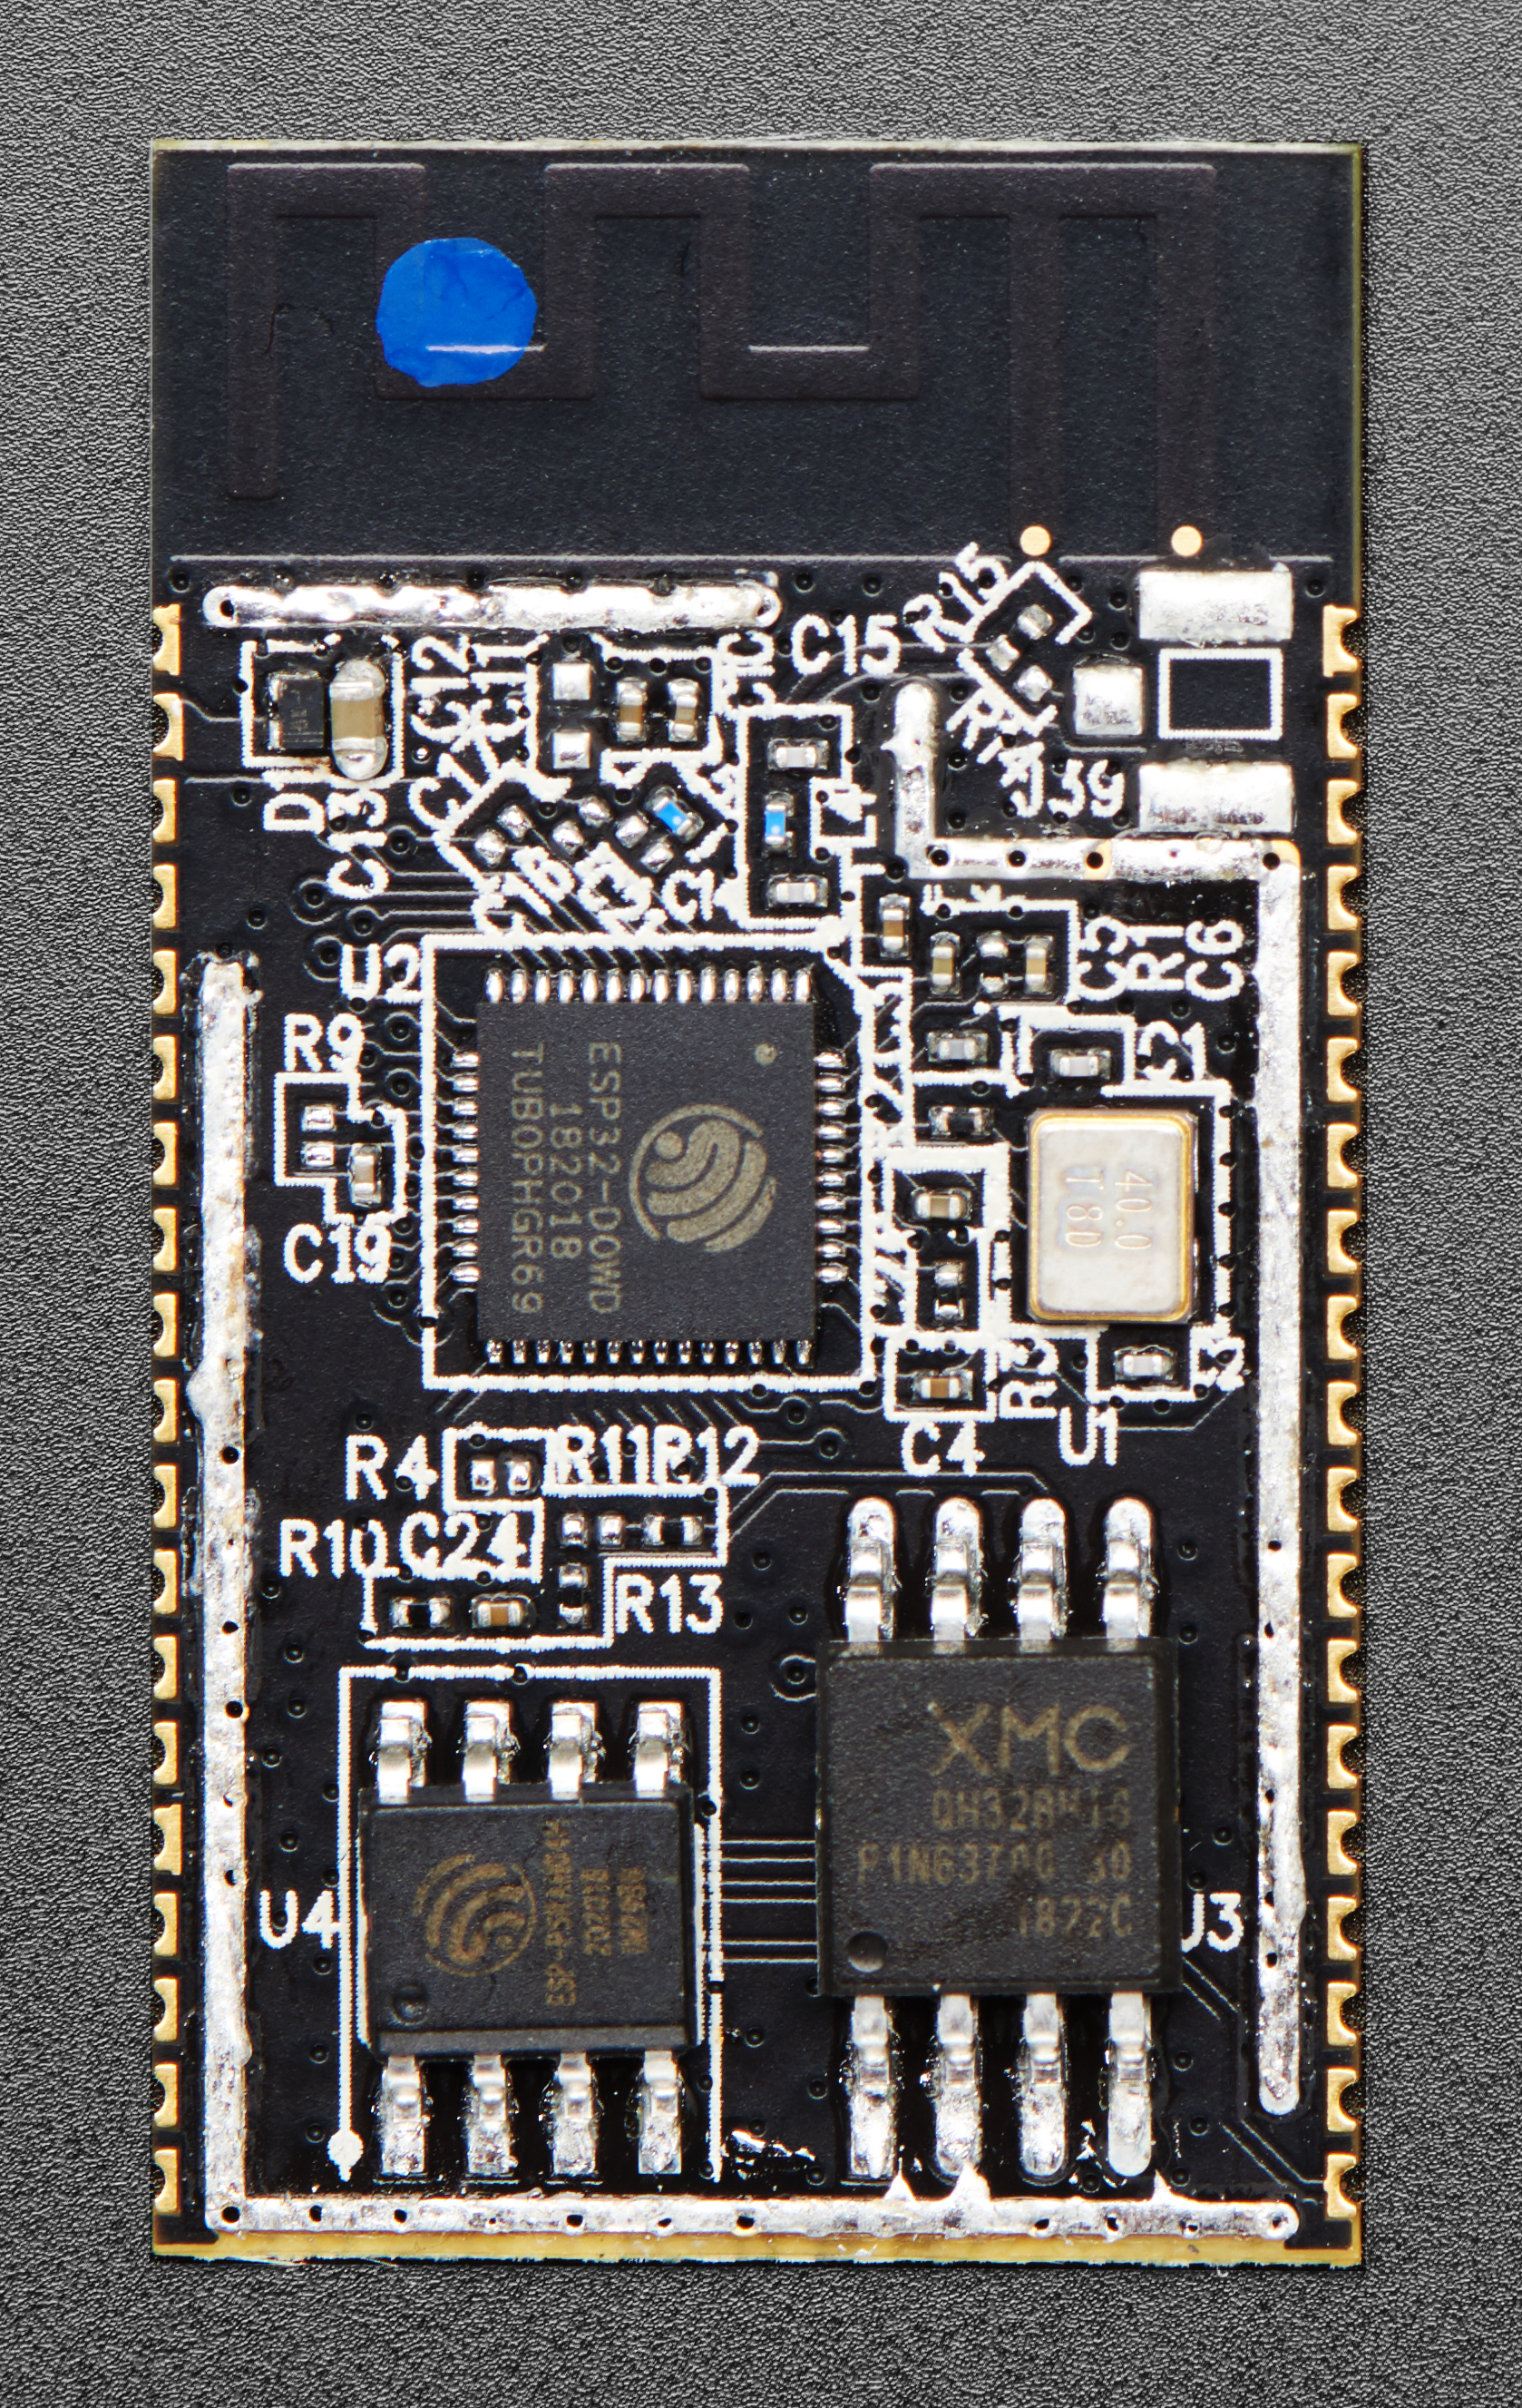
\includegraphics[width=.85\linewidth]{media/esp32_wrover_b.png}
            \subcaption{Photo of an ESP32-WROVER-B module based on the ESP32 chip \parenciteit{}{ESP32_WROVER_B:Image}}
            \label{fig:ESP32_WROVER_B}
        \end{minipage}
        \hspace{.04\linewidth}
        \begin{minipage}[H]{.5\linewidth}
            \centering
            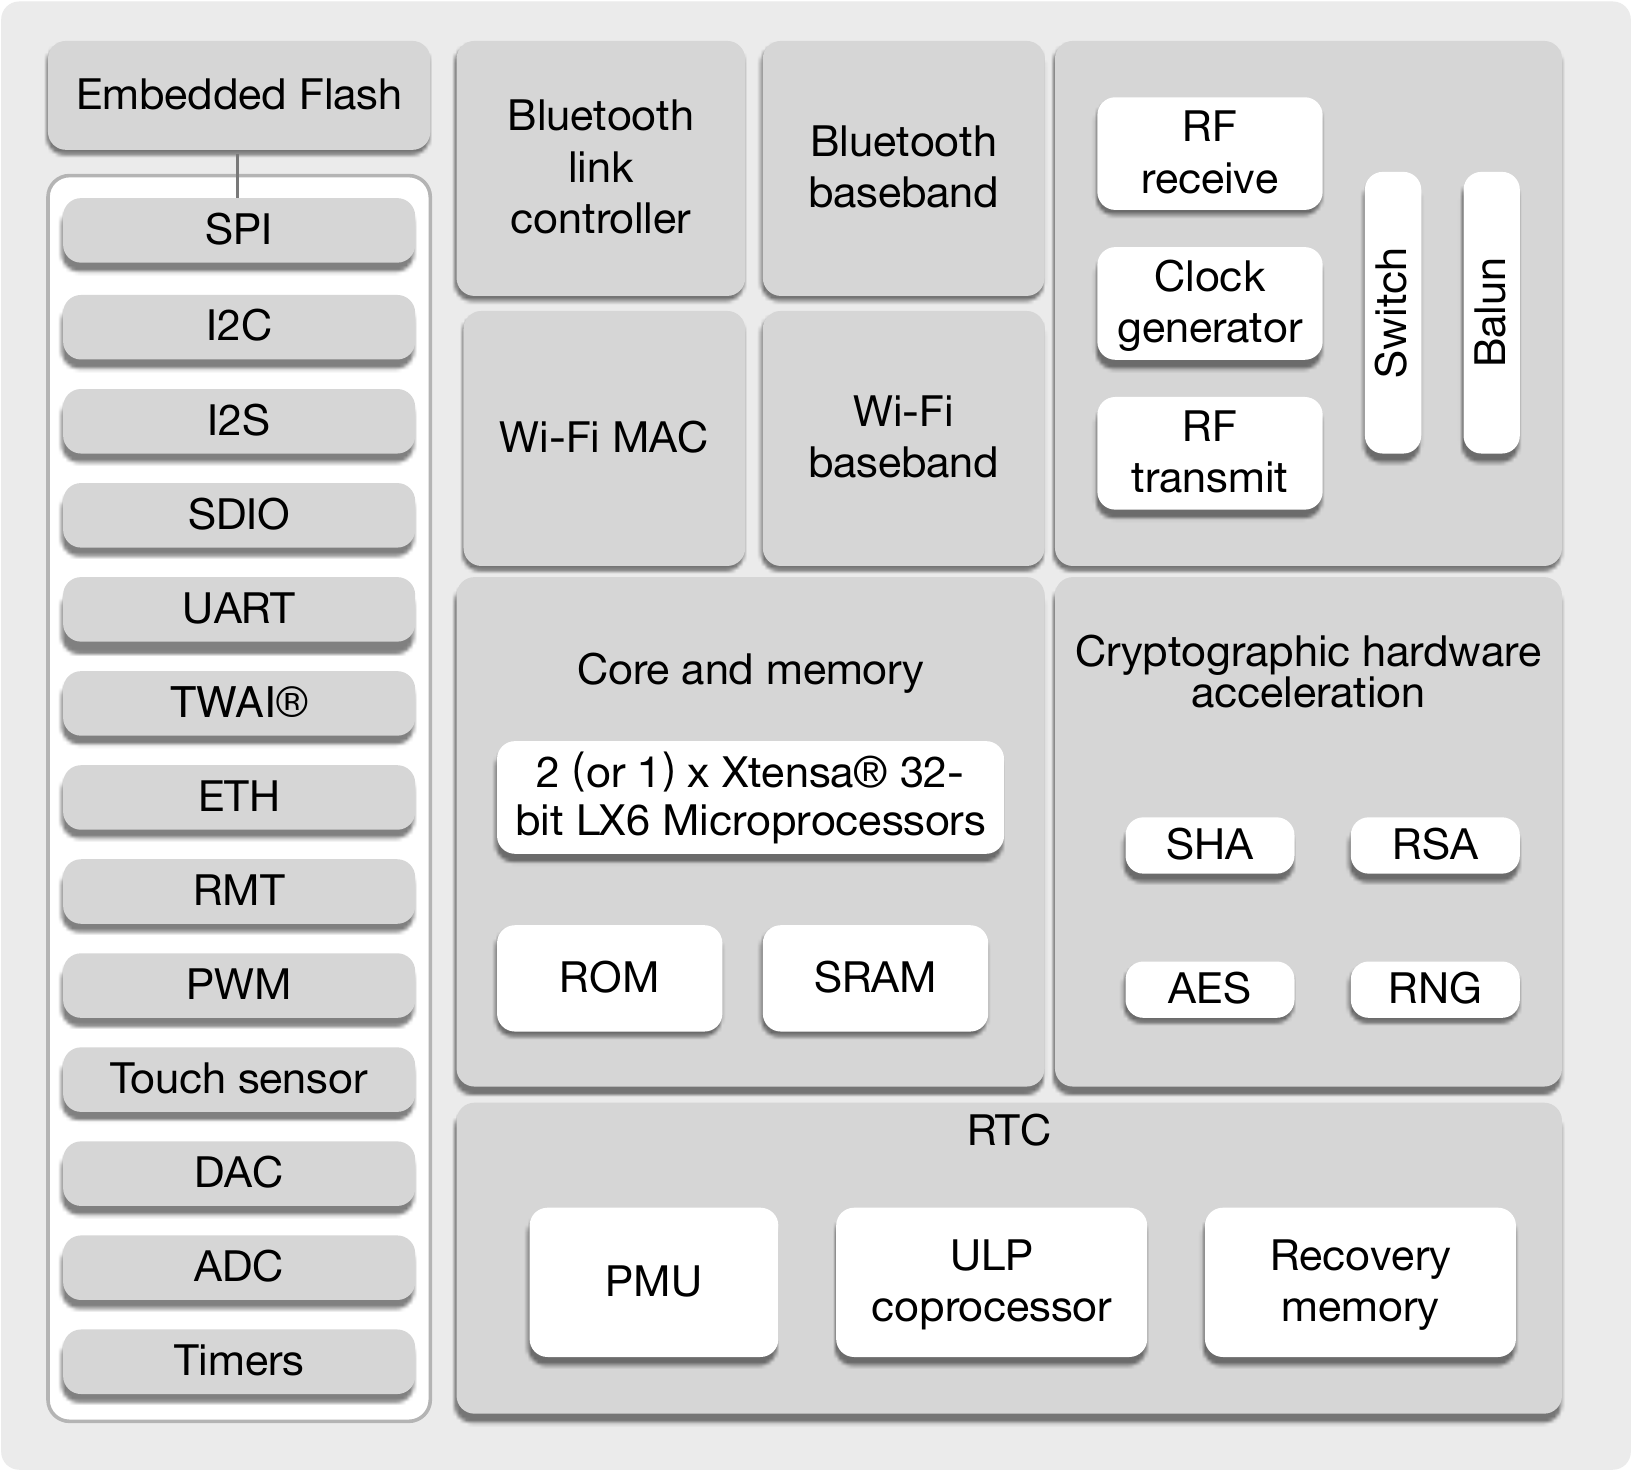
\includegraphics[width=\linewidth]{media/esp32_block_diagram.png}
            \subcaption{Block diagram of a generic chip of the ESP32 line \parenciteit{p12}{ESP32:Datasheet}}
            \label{fig:ESP32_BD}
        \end{minipage}
        \caption{}
        \label{fig:ESP32}
    \end{figure}

    \begin{figure}[!htb]
        \centering
        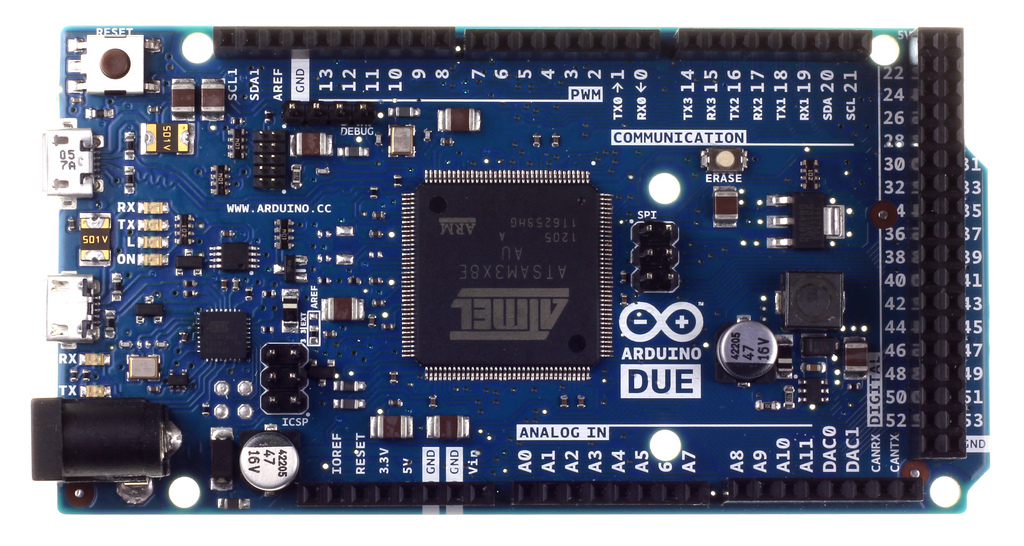
\includegraphics[width=.7\linewidth]{media/ArduinoDue_Front.jpg}
        \caption{Arduino Due board \parenciteit{}{ArduinoDue:Image}}
        \label{fig:ArduinoDue}
    \end{figure}
    \clearpage
    \todo{search for all ?? references}
    \subsubsection{Power supply}\label{sec:MotherboardDesignSupply}
    The power supply of the circuit is one of the indispensable and important parts for its correct operation, especially when analog circuits are present.
    In my case the power supply must have a voltage that is constant over time and must have relatively low noise levels\footnote{The voltage must be constant and free of interference in all possible operating modes of the circuit (i.e. with different current consumption)}.
    Consequently I must choose a topology that would create minimal interference while converting the voltage, which I could apply both in the present version and in future versions of the prototype.
    The best technique of all for this is to use a linear regulator based on the resistive principle.
    The reason behind its precision is that, to lower the voltage to the desired level, it dissipates the necessary difference as heat: this is the effect of clipping applied to the noise contained in the source\footnote{Meaning the regulator's supply}, at the expense of its own efficiency.

    The voltage of the sources, which one also tends not to change, must be such as to allow its regulation with a simple and effective battery-powered system\footnote{Meaning Li-po batteries, which have minimum voltages (without over-discharge) of $3.6V$}, to allow the ADC to communicate at the same logic voltage level\footnote{Voltage at which the chip's logic interfaces operate} as the ESP32, $3.3V$, and to power the ESP32 itself.
    The picture of using $3.3V$ is completed perfectly by the decision, for the final prototype, on a combination of a buck\footnote{A circuit that reduces voltage by means of the properties of inductance (with the possibility of galvanic isolation) with high efficiency, at the expense of the high-frequency noise introduced into the system, which increases as current consumption increases} converter to make efficient\footnote{}\todo{<-- add reference about efficency} the voltage conversion from $4.2V-3.6V$ to approximately\footnote{This value will have to be made concrete during the design of the final prototype's supply, because of the specific characteristics of the chosen components} $3.5V$, chained with linear regulators to eliminate the noise introduced by the previous stage\todo{<--add reference about reliability} and supply the required $3.3V$.
    This decision leads to the consequence that for the prototype we can use exclusively linear regulators to simulate\footnote{Because of the clipping effect of linear regulators we tend not to perceive the noise introduced into the supply by the previous stages (of course, only noise that does not go below the limit called "dropout", beyond which linear regulators stop maintaining a constant voltage): consequently those stages can be omitted} the final situation of the project and to reduce the complexity of the circuits used.

    In the concrete case of the prototype, the positive constant-voltage source is already present\footnote{The regulation is of the linear resistive type} on the Arduino DUE, which is powered by the $5V$ USB cable when the board is connected to the computer for the necessary data communication over the serial port.
    The negative source, which we will need for the filters\footnote{The reasons are discussed in Section\ref{sec:SensorBoardSchematic}}\todo{add that when we filter out DC we get a signal with a negative part}, is provided by a transformer\footnote{Figure \ref{fig:ProtoSupplyPhoto}} of $\Delta U = 12V$ without connection to the \texttt{GND}\footnote{Meaning a conductor at the $0V$ reference potential} of the outlet, galvanically isolated from the mains current so that it can be connected correctly without causing short circuits.
    The voltage is then reduced to $3.3V$ with a linear resistive regulator.
    This allows me to create two voltage sources of $3.3V$ and $-3.3$ by connecting the sources in series, with the circuit's \texttt{GND} at their junction point, as shown in Figure \ref{fig:ProtoSupplyConnection}.
    \begin{figure}[H]
        \centering
        \begin{minipage}{.44\linewidth}
            \centering
            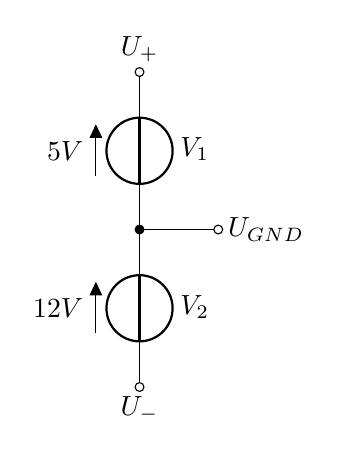
\begin{tikzpicture}[transform shape, use fpu reciprocal]
                \draw (0,0)
                    node[above]{$U_{+}$}
                    to[short, o-] ++(0,0)
                    ++(0,-2)
                    to[V=$5V$, l_=$V_1$] ++(0,2)
                    ++(0,-2)
                    coordinate(joint)
                    to[short, -o] ++(1,0)
                    node[right]{$U_{GND}$}
                    (joint) 
                    ++(0,-2)
                    to[V=$12V$, -*, l_=$V_2$] ++(0,2)
                    ++(0,-2)
                    to[short, o-] ++(0,0)
                    node[below]{$U_{-}$};
            \end{tikzpicture}
            \subcaption{Sources $V_1$ and $V_2$ are connected in series with \texttt{GND} at their center to provide $\Delta U_{GND\rightarrow +}=5V$ $\Delta U_{GND\rightarrow -}=-12V$}
            \label{fig:ProtoSupplyConnection}
        \end{minipage}
        \hspace{.04\linewidth}
        \begin{minipage}[H]{.44\linewidth}
            \centering
            % [2026 revision] replaced 4608x2229 prototype-era snapshot with a clean photo of the
            % 12V charger (was: media/album/PSX_20220227_234319.jpg — kept on disk unchanged)
            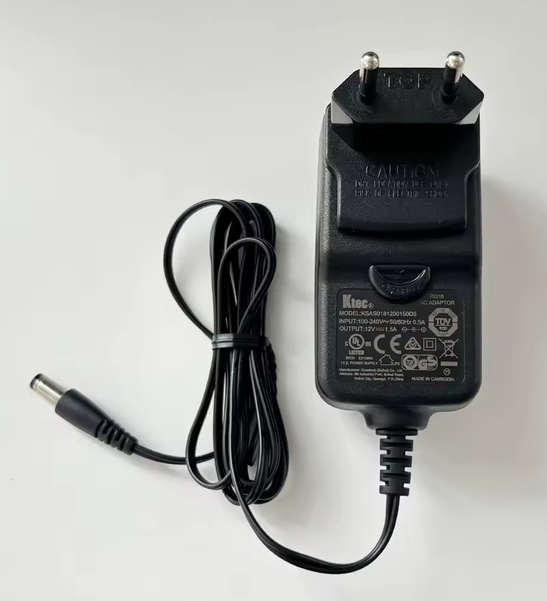
\includegraphics[width=\linewidth]{media/album/12v-charger.jpg}
            \subcaption{Power adapter I use to convert the mains voltage to $12V$, with a maximum current of $500mA$}
            \label{fig:ProtoSupplyPhoto}
        \end{minipage}
        \caption{}
        \label{fig:ProtoSuppy}
    \end{figure}
    \clearpage

    \noindent The circuit I use to reduce the voltage from $12V$ to $3.3V$ is shown in the following Figure:
    \begin{figure}[H]
        \centering
        \begin{minipage}[H]{.44\linewidth}
        \centering
        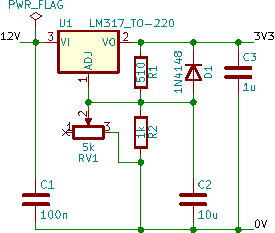
\includegraphics[page=1, width=\linewidth]{media/power_source_board_pcb_cropped.pdf}
        \subcaption{Circuit diagram drawn in the KiCad software \parenciteit{}{KiCad:Software}, where the output voltage can be varied with the potentiometer $RV1$ \emph{(The circuit was designed with reuse in future prototypes in mind, which is why there are bypass capacitors $C1$ \& $C3$, which I discuss in Section \ref{sec:SensorBoardSchematic}, and the diode $D1$ with the capacitor $C2$ to protect against short circuits)} \emph{(Partially taken from \cite[p9]{LM317:Datasheet})}}
        \label{fig:PowerSourceBoardSchematic}
        \end{minipage}
        \hspace{.04\linewidth}
        \begin{minipage}[H]{.45\linewidth}
            \centering
            \begin{minipage}[H]{\linewidth}
                \centering
                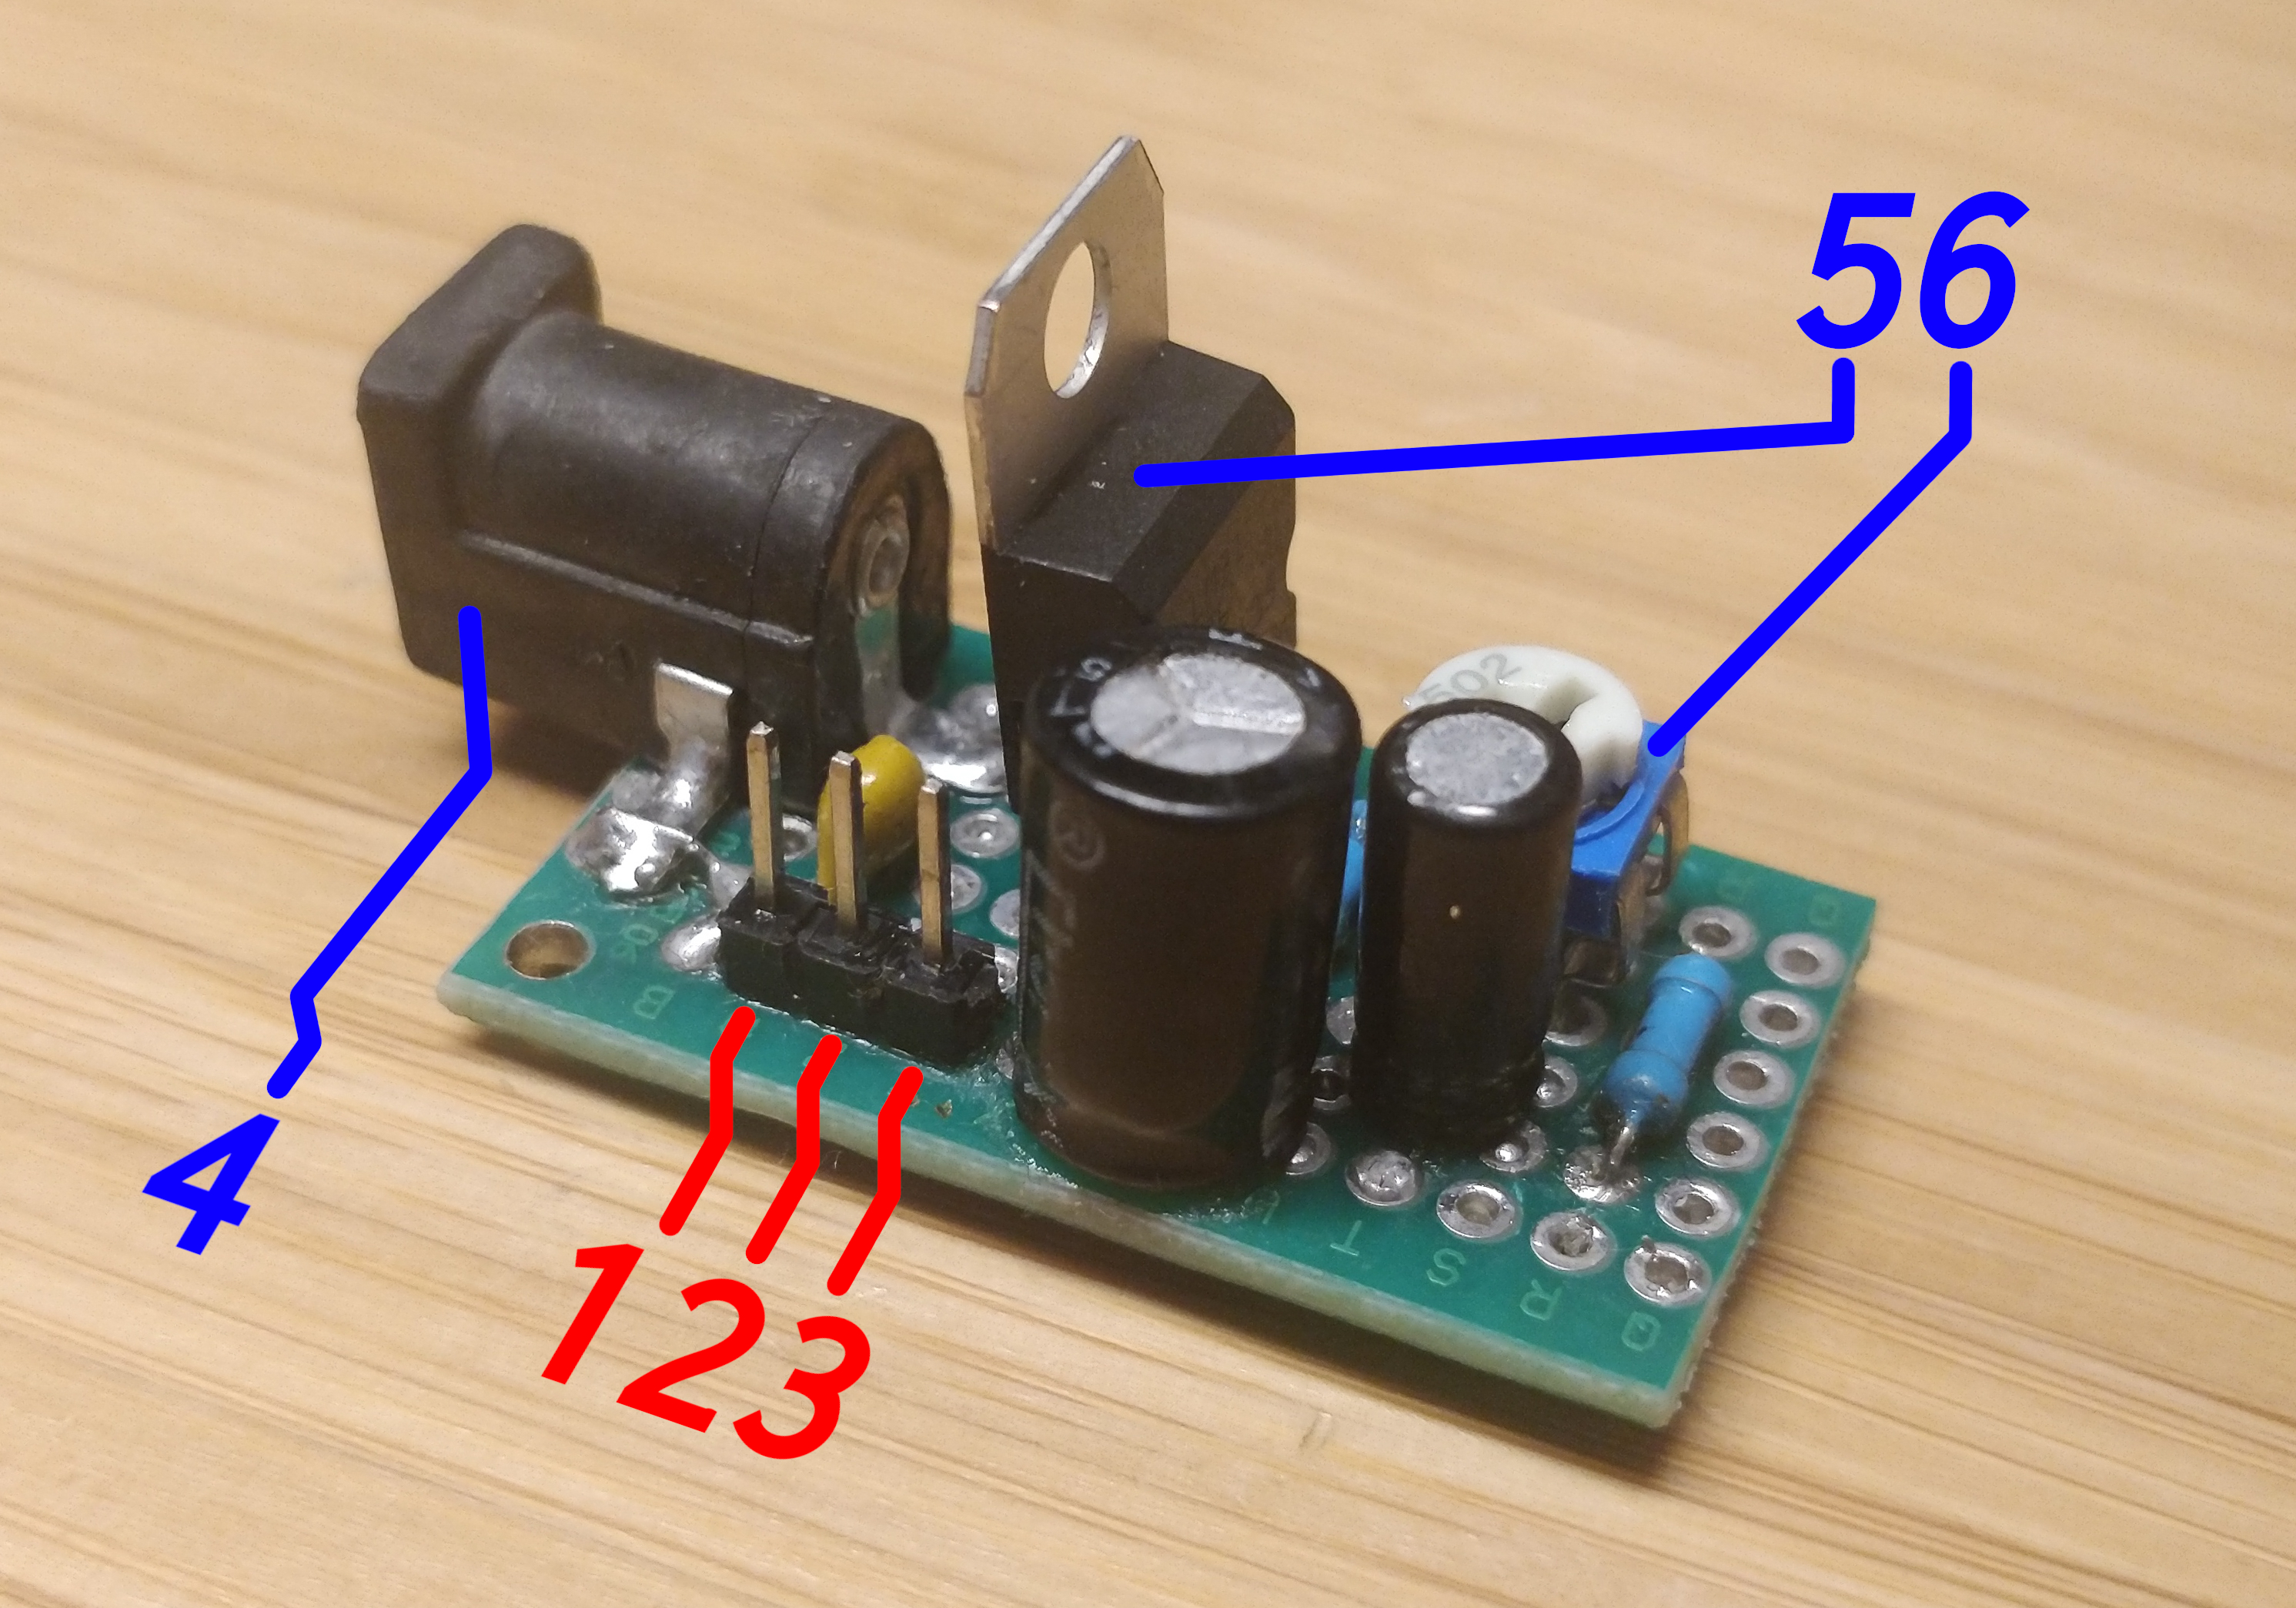
\includegraphics[width=.66\linewidth]{media/album/PSX_20220227_234533_ed.jpg}
                \subcaption{Regulator board and its components. In red: $1$ - $0V$ pin, $2$ - $12V$ pin, $3$ - $3V3$ pin. In blue: $4$ - power adapter connector, $5$ - LM317, $6$ - potentiometer $RV1$ \emph{(At the time of construction I did not have the ceramic capacitor $C3$ and replaced it with an electrolytic one)}}
                \label{fig:PowerSourceBoardPhoto}
            \end{minipage}
            \\
            \begin{minipage}[H]{\linewidth}
                \centering
                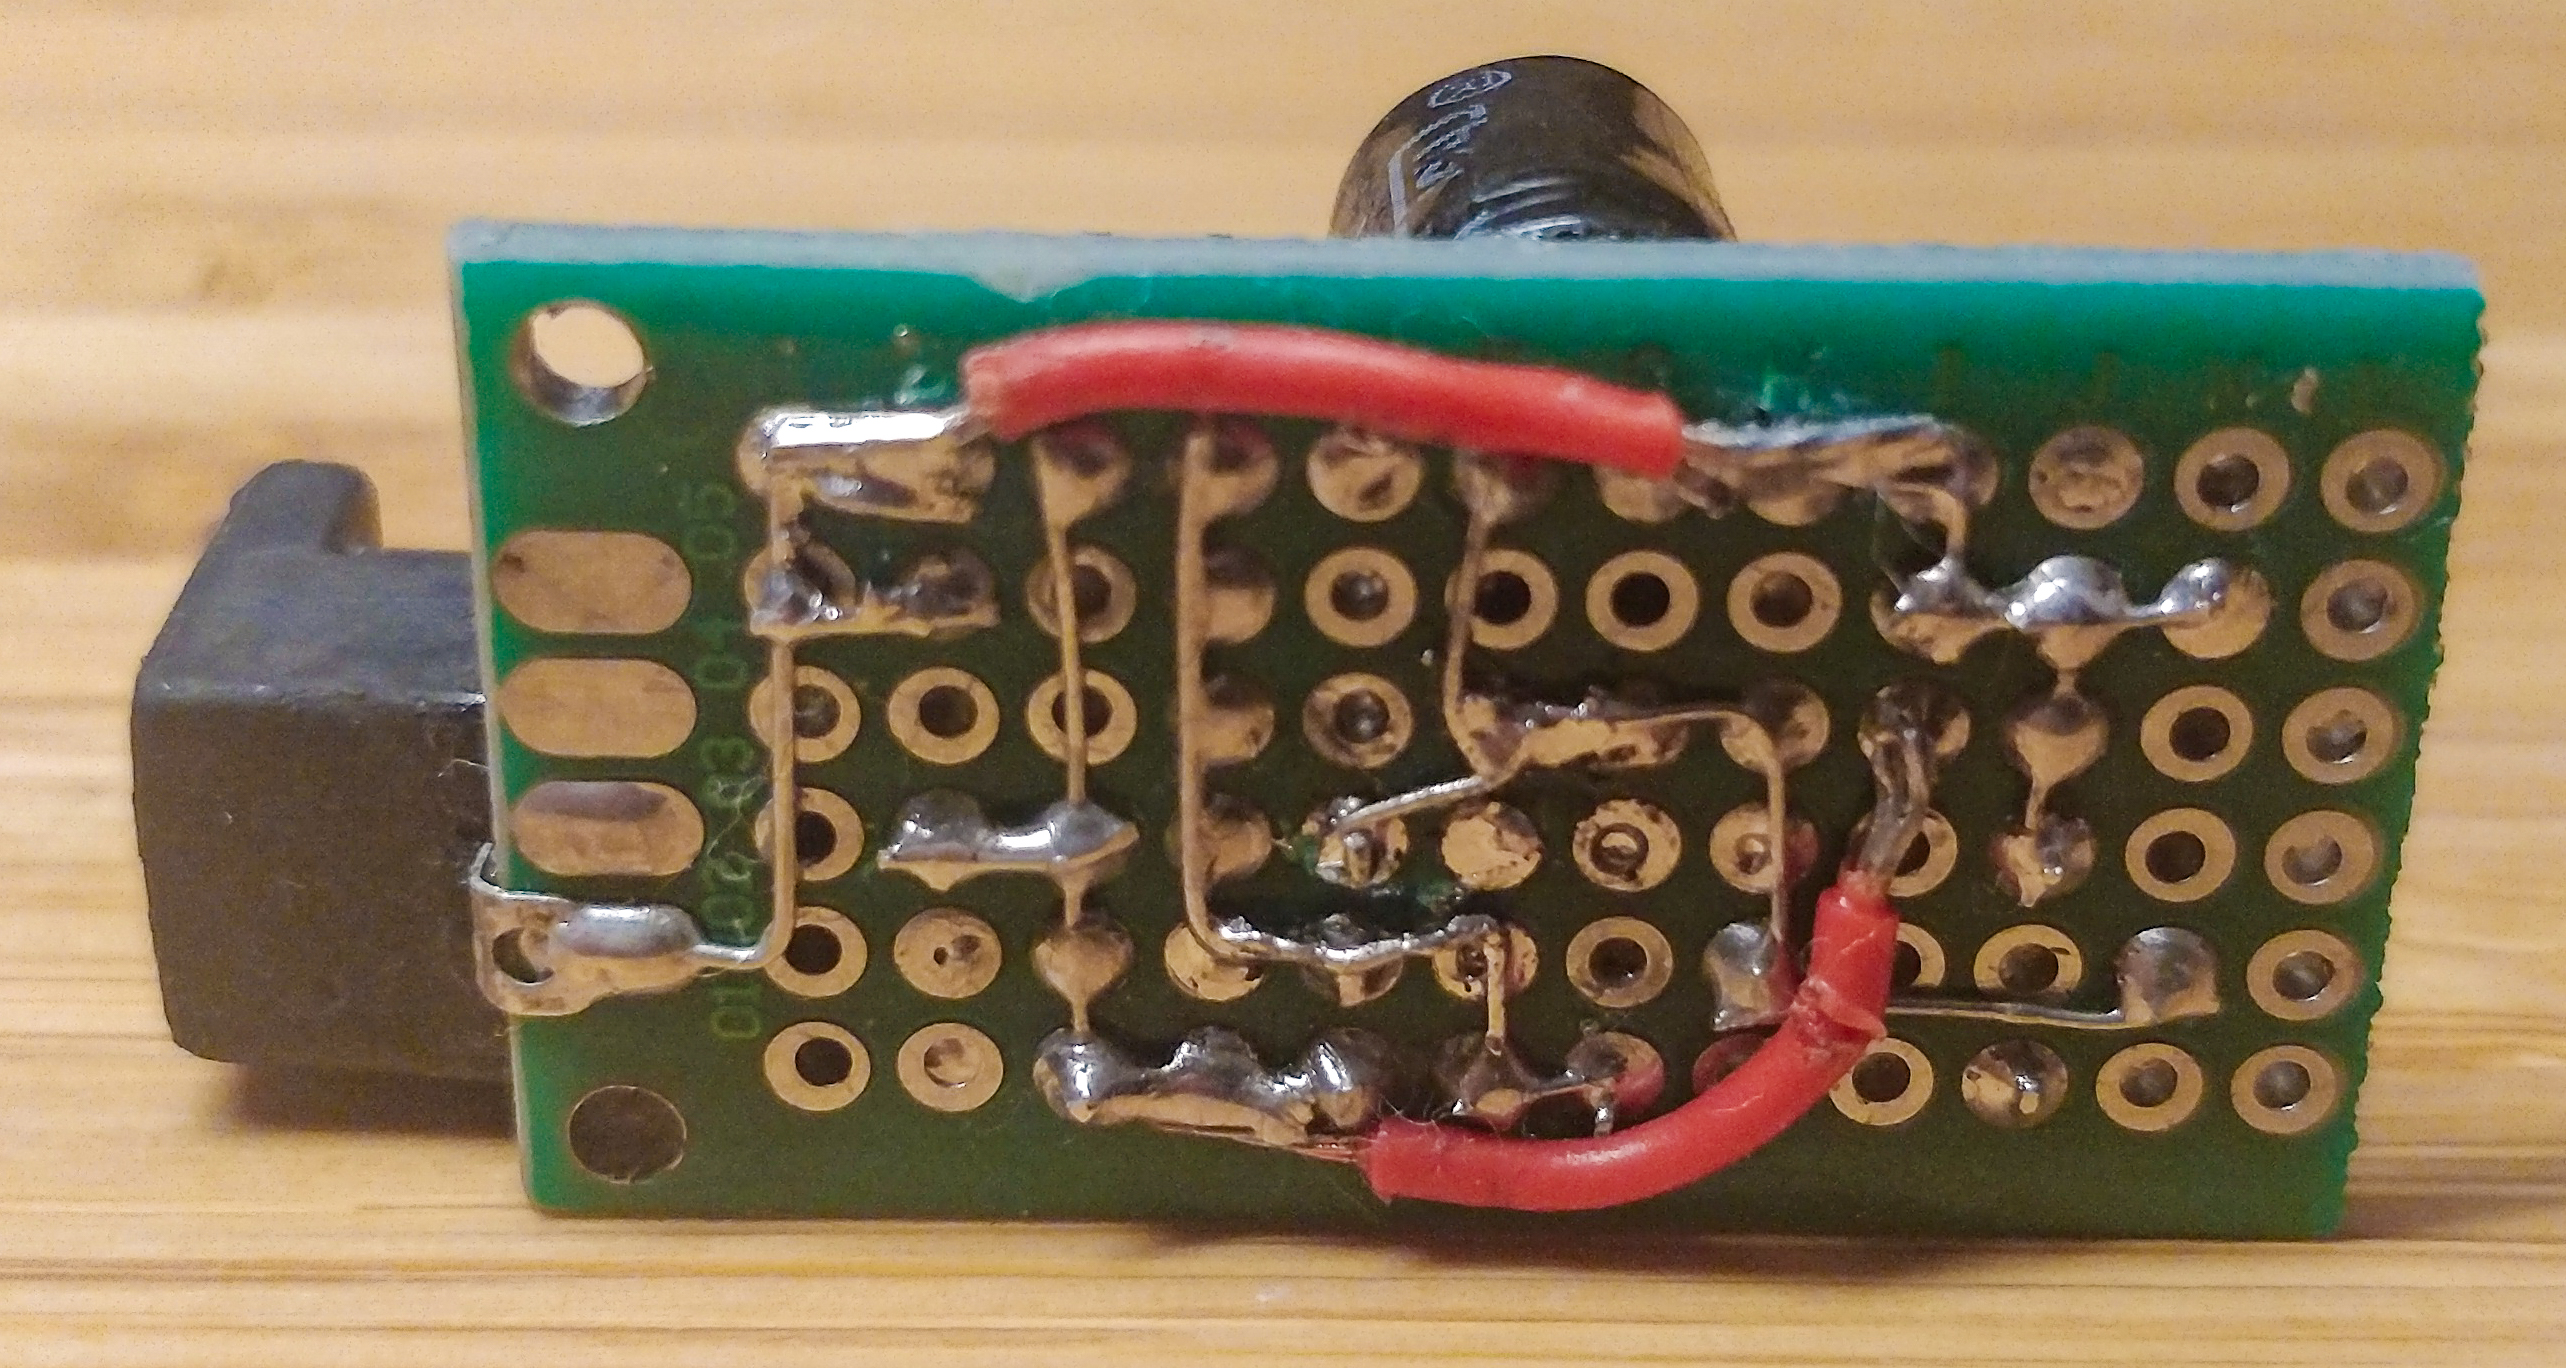
\includegraphics[width=.8\linewidth]{media/album/PSX_20220227_234420.jpg}
                \subcaption{Component connections on the back of the regulator board: the circuit was soldered with THT \emph{(Through Hole Technology)} to reduce the time spent on design and construction}
                \label{fig:PowerSourceBoardPhotoBack}
            \end{minipage}
        \end{minipage}
        \caption{Adjustable linear regulator board ($1.25V-3.375V$) based on the LM317 \parenciteit{}{LM317:Datasheet}}
        \label{fig:PowerSourceBoard}
    \end{figure}
    \todo{add reference to the project's GitHub}
    \noindent The calculations needed to determine the resistors are the following:
    
    \begin{figure}[H]
        \centering
        \begin{minipage}[H]{.15\linewidth}
            \[U_{out} \approx 3.3V\]
        \end{minipage}
        \begin{minipage}[H]{.15\linewidth}
            \[U_{ref}=1.25V\]
        \end{minipage}
        \begin{minipage}[H]{.15\linewidth}
            \[R_2=1k\Omega\]
        \end{minipage}
        \begin{minipage}[H]{.15\linewidth}
            \[RV_1=5k\Omega\]
        \end{minipage}
        \begin{minipage}[H]{.15\linewidth}
            \[I_{adj}=100\mu A\]
        \end{minipage}
        \begin{minipage}[H]{\linewidth}
            \vspace{3ex}
            \[U_{out}=U_{ref}\left(1+\frac{RV_1 \parallel R_2}{R_1}\right)+I_{adj} \left(RV_1 \parallel R_2\right)\]
        \end{minipage}
    \end{figure} \todo{add reference on how to make the parallel sign in the circuit}
    \noindent $I_{adj}$ is the current flowing through the \texttt{ADJ} pin of the LM317 regulator; as can be seen, it affects $U_{out}$, but with a balanced choice of resistor values its effect tends to be small.
    The resistor values are to be chosen according to the standardized E series of values\footnote{The values apply not only to resistors but also to capacitors}\:\footcite[]{ESeries:Wiki}.
    After some searching among components I already had and some trial and error with the calculations, I arrived at the values\footnote{The capacitor values were taken directly from the source of the diagram in Figure \ref{fig:PowerSourceBoardSchematic}} shown in the circuit diagram in Figure \ref{fig:PowerSourceBoardSchematic}.
    \clearpage

    \section{Filters - Theory}\label{sec:FilterTheory}
    By the term "filters", also taking into account the content of Section \ref{sec:SensorboardDesignInput} and Section \ref{sec:SensorboardDesignOutput}, frequency filters are meant, which conveniently\footnote{The reason is discussed in Section \ref{sec:ElectronicsCalculusLaplace}} belong to LTI systems\footnote{The term and its meaning are discussed in the next Section, Section \ref{sec:FilterTheorySystems}}.

    \subsection{Systems}\label{sec:FilterTheorySystems}
    When I mention \emph{Input} and \emph{Output}, I refer to the concept of systems given by systems and control theory\footcite[]{ControlTheory:Wiki}.
    The theory is useful in our case because it provides a model through which we can design a system\footnote{A system is initially an abstract concept of a subject that processes inputs to give outputs, which can then be implemented} that would allow us to reach desired states of some number of \emph{Outputs} through states of some number of \emph{Inputs} in the most optimal way possible.

    \begin{samepage}
        \noindent There are different categories of systems given by their characteristics, but we are interested only in a specific one, into which our filter falls:
        \begin{enumerate}[label=\emph{(\arabic*)}]
            \item Interface type: SISO, i.e. Single Input Single Output\footnote{One input, one output}
            \item System type: LTI, i.e. Linear Time Invariant\footnote{Linear and invariant over time}
        \end{enumerate}
    \end{samepage}
    The name of the first characteristic speaks for itself, while the second characteristic may seem less clear.
    The two concepts that LTI encompasses, linearity and time invariance, need to be discussed.

    By itself, the characteristic of linearity can appear in various systems if they are not used at the physical limit they were designed for, even though, predominantly, real-world systems tend to be non-linear\footcite[]{TransferFunction:Wiki}.
    \begin{samepage}
        \noindent Concretely, the concept of linearity is described by the satisfaction of two conditions:
        \begin{enumerate}[label=\emph{(\arabic*)}]
            \item Additivity, described by the following formula: \[f(x + y) = f(x) + f(y)\]
            \item Homogeneity, described by the following formula: \[f(a \cdot x) = a \cdot f(x)\]
        \end{enumerate}
    \end{samepage}

    A real example of a linear system can be a circuit, as in Figure \ref{fig:ExampleLTICircuit}, containing a transistor\footnote{In this example we consider a MOSFET}, whose \emph{Output} will behave linearly\footnote{This can be seen in Figure \ref{fig:ExampleLTIIRFZ44N_Plot_Vgs}} with the variation of the voltage\footnote{The phenomenon occurs with MOSFETs, but not all transistors work the same way} at the \emph{Input} if it is operated in the saturation region.
    % TRANSLATOR NOTE: the inline-math subscript $V_{DS_{saturazione}}$ (also next line) is Italian but left untouched per the math-mode rule; consider $V_{DS_{\mathrm{sat}}}$.
    The saturation region, which can be identified in Figure \ref{fig:ExampleLTIIRFZ44N_Plot_Vds}, is a range of voltages $U_{out}$ (corresponding to $V_{DS}$) for $V_{DS_{saturazione}} < V_{DS}$ for which the transistor behaves linearly with the variation of the voltage $U_{in}$\footnote{It must also be taken into account because it is a parameter of the function shown in the plot: increasing $V_{GS}$ increases the voltage $V_{DS_{saturazione}}$} (corresponding to $V_{GS}$).
    If, instead, the circuit is operated in the triode region, the range of $V_{DS}$ for $0 < V_{DS} < V_{DS_{saturazione}}$, $I_D$ starts to depend on $V_{DS}$ or $U_{out}$ as well: with this behavior the circuit violates the two conditions defined by linear behavior, thereby becoming a non-linear system.
    \begin{figure}[H]
        \centering
        \begin{minipage}{.84\linewidth}
            \centering
            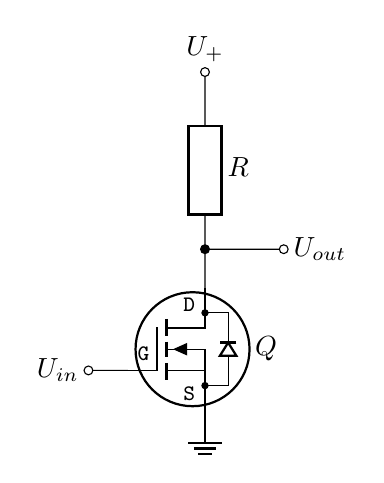
\begin{tikzpicture}[transform shape, use fpu reciprocal]
                \draw (0,0)
                    node[above]{$U_{+}$}
                    to[short, o-] ++(0,-.25)
                    to[R, l=$R$, -*] ++(0,-2)
                    coordinate(joint)
                    to[short, -o] ++(1,0)
                    node[right]{$U_{out}$}
                    (joint) to[short] ++ (0,-.5)
                    node[nigfete, anchor=D, bodydiode, tr circle] (fet) {$Q$}
                    (fet.S) node[anchor=south east] {\footnotesize{\texttt{S}}}
                    (fet.D) node[anchor=north east] {\footnotesize{\texttt{D}}}
                    (fet.G) node[anchor=south west] {\footnotesize{\texttt{G}}}
                    (fet.S) node[ground]{} ++(0,-.5)
                    (fet.G) to[short, -o] ++(-.5,0)
                    node[left]{$U_{in}$};
            \end{tikzpicture}
            \subcaption{The IRFZ44N is named $Q$ \emph{(}\texttt{G}\emph{ = Gate, }\texttt{D}\emph{ = Drain, }\texttt{S}\emph{ = Source)}, an ideal resistor $R$, a constant voltage source $U_{+}$, the \emph{Input} $U_{in}$ and the \emph{Output} $U_{out}$}
            \label{fig:ExampleLTICircuit}
        \end{minipage}
        \\
        \vspace{3ex}
        \begin{minipage}[t]{.4\linewidth}
            \centering
            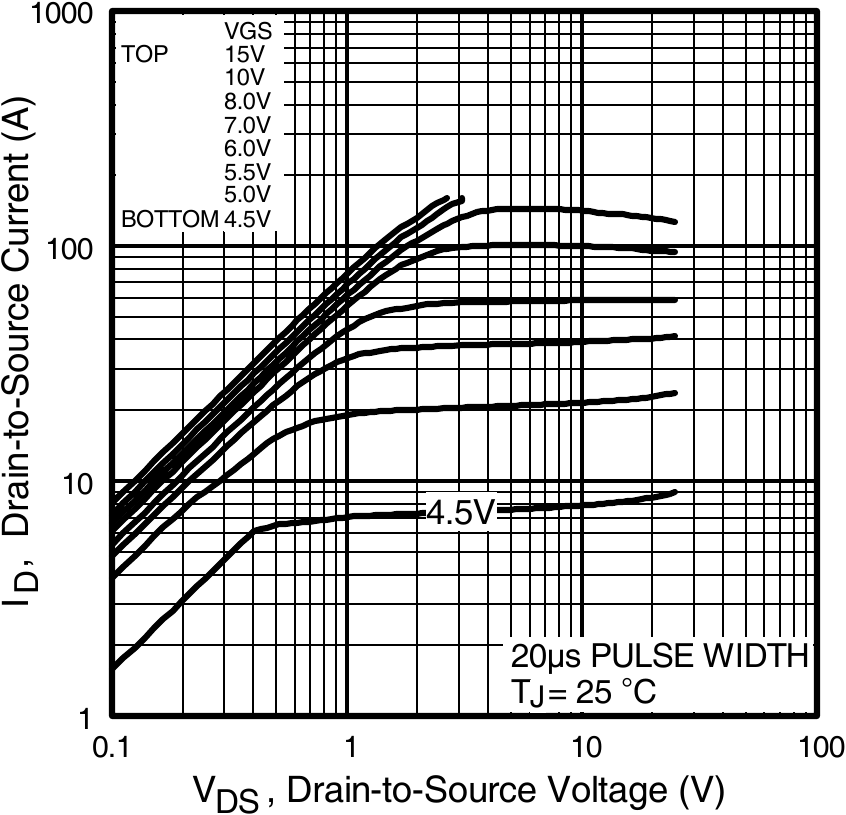
\includegraphics[width=\linewidth]{media/irfz44n_vds_id_plot.png}
            \subcaption{Variation of $I_D$ as a function of $V_{DS}$ with parameter $V_{GS}$ \emph{(the saturation region is defined for $V_{DS}$ beyond the point where $I_D$ approximately stops growing)}}
            \label{fig:ExampleLTIIRFZ44N_Plot_Vds}
        \end{minipage}
        \hspace{.04\linewidth}
        \begin{minipage}[t]{.4\linewidth}
            \centering
            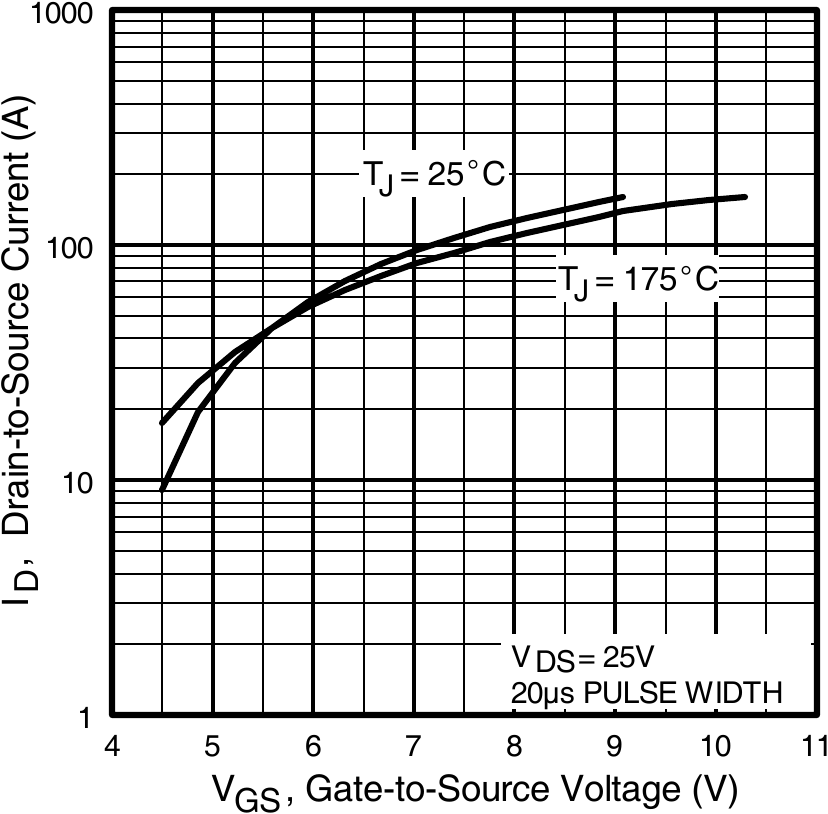
\includegraphics[width=\linewidth]{media/irfz44n_vgs_id_plot.png}
            \subcaption{Variation of $I_D$ as a function of $V_{GS}$ in the saturation region for \emph{($V_{DS} = 25V$)}, which is approximately linear}
            \label{fig:ExampleLTIIRFZ44N_Plot_Vgs}
        \end{minipage}
        \caption{Example of an amplifier based on an IRFZ44N \emph{(A transistor, more specifically an N-channel enhancement-mode MOSFET)} \parenciteit{}{IRFZ44N:Datasheet} with the corresponding circuit in \ref{fig:ExampleLTICircuit} and the plots \parenciteit{}{IRFZ44N:Datasheet} of the current-voltage characteristics in \ref{fig:ExampleLTIIRFZ44N_Plot_Vds}, \ref{fig:ExampleLTIIRFZ44N_Plot_Vgs}}
        \label{fig:ExampleLTI}
    \end{figure}


    The concept of time invariance is given by the consistency of the system's results over time: to be considered time-invariant, the system must not give different \emph{Outputs} for the same \emph{Inputs} at different moments.

    A good example of a time-variant system could be a website that shows time zones in real time.
    If the date and time of a specific time zone are requested, each time the values received will differ from those requested at a later moment.


    The reasons why the analog frequency filter we need is considered an LTI system lie in the property of analog circuits of tending to easily describe certain time-invariant systems\footnote{The time variance of an electronic system designed to be invariant, like its linearity, can depend on physical phenomena such as changes in resistance at different temperatures, or EMI} and of being linear in their response if not used outside the designed parameters, such as the saturation voltage of the MOSFET in the previous example.
    An additional piece of information is that time variance can make sense in signal processing terms when digital systems are used, where the data are not strictly bound to time but are discrete.

    The real advantage of having classified the filter as an LTI system becomes apparent once their properties\footnote{The properties and the relations between them are discussed in Section \ref{sec:TransformsAndLaplace}} are understood, namely the possibility of describing the system with an impulse and, as a direct consequence of this first fact, being able to represent the system with a function, called the transfer function.
    \clearpage

    \subsection{Mathematics \& Physics} \label{sec:MathAndPhysics}
    I mentioned transfer functions\footcite[]{TransferFunction:Wiki} in the previous sections\footnote{Section \ref{sec:IntroFiltersSignals} and Section \ref{sec:FilterTheorySystems}} and their characteristic of being an abstraction of the filter.
    \begin{samepage}
        The following equalities must be taken into account:
        \begin{figure}[H]
            \centering
            \begin{minipage}[b]{.35\linewidth}
                \centering
                \[
                    H(s) = \frac{Output}{Input} = \frac{U_{out}}{U_{in}}
                \]
            \end{minipage}
            \begin{minipage}[b]{.35\linewidth}
                \centering
                \[
                    s = j\omega\ + \sigma
                \]
            \end{minipage}
        \end{figure}
    \end{samepage}

    Transfer functions, generally denoted by the capital letter $H(s)$ in mathematical function notation, are functions that describe the relation between a domain, i.e. \emph{Input}, and a codomain, i.e. \emph{Output}, as a function of the complex variable $s$, relating the \emph{Input} and the \emph{Output} by dividing one by the other.
    Moreover, knowing that the signal we are studying is described by voltage variations, we make the \emph{Input} correspond to $U_{in}$ and the \emph{Output} to $U_{out}$.

    In physics and mathematics terms we know that $j$, which in our case represents the imaginary unit \(i\), is multiplied by $\omega$, thus forming the imaginary part of $s$, under the condition $\Im(\omega) = 0$.
    \(\sigma\), instead, forms the real part of \(s\), again under the identical condition $\Im(\sigma) = 0$.

    \noindent A transfer function can also be described by two polynomials, $N_n(x)$ in the numerator and $D_m(y)$ in the denominator, as follows:
    \begin{figure}[H]
        \centering
        \begin{minipage}[b]{.3\linewidth}
            \centering
            \[
                N_n(x) = \sum^{n}_{k=0} a_k x^k \mathrm{,}
            \]
        \end{minipage}
        \begin{minipage}[b]{.3\linewidth}
            \centering
            \[
                D_m(y) = \sum^{m}_{j=0} b_j y^j \mathrm{,}
            \]
        \end{minipage}
        \begin{minipage}[b]{.3\linewidth}
            \centering
            \[
                H(s) = \frac{N_n(s)}{D_m(s)}
            \]
        \end{minipage}
    \end{figure}
    \noindent Then $H(s)$ can be rewritten with polynomials in expanded or factored form
    \begin{figure}[H]
        \centering
        \begin{minipage}[b]{.45\linewidth}
            \centering
            \[
                H(s) = \frac{a_0 + a_1 s + \dotsm + a_{n-1} s^{n-1} + a_n s^n}{b_0 + b_1 s + \dotsm + b_{m-1} s^{m-1} + b_m s^m} \mathrm{,}
            \]
        \end{minipage}
        \hspace{0.04\linewidth}
        \begin{minipage}[b]{.45\linewidth}
            \centering
            \[
                H(s) = \frac{z_0 \left(s - z_1\right) \dotsm \left(s^{n-1} - z_{n-1}\right) \left(s^n - z_n\right)}{p_0 \left(s - p_1\right) \dotsm \left(s^{m-1} - p_{m-1}\right) \left(s^m - p_m\right)}
            \]
        \end{minipage}
    \end{figure}
    \noindent and substituting into the equality the expression $K = \frac{z_0}{p_0}$, which corresponds to the gain coefficient\footnote{We will need this variable later} \todo{Review the footnote for references}
    \begin{figure}[H]
        \centering
        \[
            H(s) = K \frac{\left(s - z_1\right) \left(s^2 - z_2\right) \dotsm \left(s^{n-1} - z_{n-1}\right) \left(s^n - z_n\right)}{\left(s - p_1\right) \left(s^2 - p_2\right) \dotsm \left(s^{m-1} - p_{m-1}\right) \left(s^m - p_m\right)}
        \]
    \end{figure}
    \noindent From the equalities it follows:
    \begin{figure}[H]
        \centering
        \begin{minipage}[b]{.3\linewidth}
            \centering
            \[
                \lim_{s \to z_i} H(s) = 0
            \]
        \end{minipage}
        \hspace{0.04\linewidth}
        \begin{minipage}[b]{.3\linewidth}
            \centering
            \[
                \lim_{s \to p_i} H(s) = \infty
            \]
        \end{minipage}
    \end{figure}
    % TRANSLATOR NOTE: original calls poles "picchi" (peaks); translated with the standard term "poles" here and below.
    \noindent For every $s$ that tends to the values $z_i$, logically named "\emph{zeros}", the value of the function $H(s)$ tends to $0$, while when $s$ tends to $p_i$, no less logically named "\emph{poles}", $H(s)$ becomes $\infty$.
    From then on we can describe transfer functions using only \emph{zeros}, \emph{poles} and $K$, the gain constant.

    The characteristic of the transfer function that would be useful to us \todo{Add end reference for the order of filters} in the physical part is the order of the transfer function.
    % TRANSLATOR NOTE: the display-math line below read "ordine = m"; changed the Italian word to "order" (only math-mode edit in the file).
    The order is given by the number of poles present in the function:
    \[
        order = m
    \]

    To understand the modifications made to the \emph{Input} of the function, the complex number $s$ can be represented on the plane with $\omega$ on the real axis and $\sigma$ on the imaginary axis, thus constructing a so-called "\emph{s-plot}"\footnote{Figure \ref{fig:ExampleSPlot}}, on which we can mark the \emph{poles} with crosses and the \emph{zeros} with small circles.

    \begin{figure}[!htb]
        \centering
        \hspace{0.15\textwidth}
        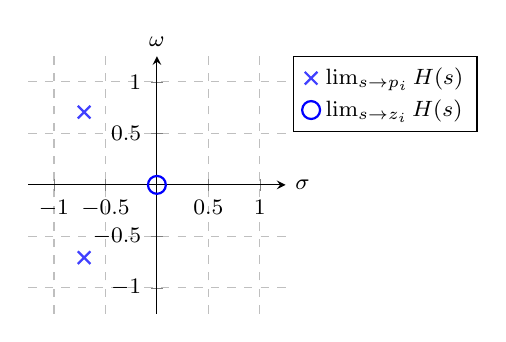
\begin{tikzpicture}
            \begin{axis}[
                axis x line=middle,
                axis y line=middle,
                xlabel={$\sigma$},
                ylabel={$\omega$},
                legend entries={$\lim_{s \to p_i} H(s)$, $\lim_{s \to z_i} H(s)$},
                legend pos=north east,
                height=.4\textwidth,
                width=.4\textwidth,
                clip=true,
                xtick distance=.5,
                ytick distance=.5,
                xmin=-1.25,
                xmax=1.25,
                ymin=-1.25,
                ymax=1.25,
                ymajorgrids=true,
                xmajorgrids=true,
                grid style=dashed,
                axis_style_default
            ]
            \addplot[
                only marks,
                color=blue!75,
                mark size=.75ex,
                thick,
                mark=x
            ]
                coordinates{(-0.707,0.707)(-0.707,-0.707)};
            \addplot[
                only marks,
                color=blue,
                mark size=.75ex,
                thick,
                mark=o
            ]
                coordinates{(0,0)};
            \end{axis}
        \end{tikzpicture}
        \caption{Example of an s-plot of $H(s)$, a second-order function}
        \label{fig:ExampleSPlot}
    \end{figure}
    
    Continuing the reasoning, let us answer what \(\omega\) corresponds to.
    In physics \(\omega\) frequently denotes angular frequency, i.e. frequency measured in \([\frac{rad}{s}]\) rather than \([Hz]\). The relation is simple:
    \[ \omega = 2\pi\cdot f\]

    Meanwhile, \(\sigma\), from a physical point of view, indicates the signal growth coefficient, the meaning of which is much easier to understand if \(\zeta\) is used in its place, which presents itself as a classic damping coefficient of a harmonic motion.
    \[ \sigma = -\zeta\]

    \begin{samepage}
        \noindent To better understand the influence of $\zeta$ on an \emph{Input}, I propose an example in Figure \ref{fig:ExampleDampingAndFrequencyDifference}
        \begin{figure}[H]
            \centering
            \begin{tikzpicture}
                \begin{axis}[
                    axis x line=middle,
                    axis y line=middle,
                    xlabel={$x$},
                    ylabel={$y$},
                    legend entries={$(a)$ $\zeta=0.1$, $(b)$ $\zeta=0.2$, $(c)$ $\zeta=0.6$},
                    legend pos=north east,
                    height=.4\textwidth,
                    width=.9\textwidth,
                    clip=true,
                    domain=0*pi:7*pi,
                    x_axis_style_pi=2,
                    ytick distance=0.5,
                    xmin=0,
                    xmax=20,
                    ymin=-1.1,
                    ymax=+1.1,
                    smooth,
                    ymajorgrids=true,
                    xmajorgrids=true,
                    grid style=dashed,
                    axis_style_default
                ]
                \addplot [thick, color=gray!75] {1.00503 * sin(x * 0.99498) * (2.71828 ^(-0.1 * x)) };
                \addplot [thick, color=blue!75] {1.02062 * sin(x * 0.97979) * (2.71828 ^(-0.2 * x)) };
                \addplot [thick, color=red!75]  {1.25    * sin(x * 0.8)     * (2.71828 ^(-0.6 * x)) };
            \end{axis}
            \end{tikzpicture}
            \caption{Example of three signals of a second-order system with $\omega=1$, generated by the response to an impulse function $\delta(x)$ \emph{(a function, also called "Dirac delta", which equals $y = 0$ for any $x$ except at $x = 0$, where $y = +\infty$)} \parenciteit{}{Impulse:Wiki}}
            \label{fig:ExampleDampingAndFrequencyDifference}
        \end{figure}
    \end{samepage}

    It nevertheless remains unknown how to convert the transfer function, which is expressed as a function of the values $s$, into one that takes values of time $t$ and that would describe the reaction to a signal, which can be either an impulse, as in Figure \ref{fig:ExampleDampingAndFrequencyDifference}, or any other type of signal.
    For these cases one should turn first to the topic of transforms in general and then specifically to the Laplace transform.

    \begin{samepage}%
        \subsubsection{Transforms \& Laplace} \label{sec:TransformsAndLaplace}
        Let us start from the definition of a transform\footnote{Also called "integral transformation" or "integral transform"}: \nopagebreak
        \begin{figure}[H]
            \Centering
            \vspace{1ex}
            \textit{"An integral transform maps a function from its original function space into another function space via integration, where some of the properties of the original function might be more easily characterized and manipulated than in the original function space." }

            \RaggedLeft
            \vspace{1ex}

            \scriptsize{\parenciteit{}{Transform:Wiki}}
            \vspace{1ex}
        \end{figure}
        \noindent Rephrasing, transforms serve to change the domain of functions in order to work with them more conveniently.
    \end{samepage}%

    \begin{samepage}%
        Let us start first of all from transfer functions, i.e. the "\emph{Input}" of the transforms: transfer functions are originally given by differential equations\footnote{I propose an example in Section \ref{sec:ElectronicsCalculusLaplace}} that describe the behavior of the output signal in relation to the input signal in the time domain, such as:
        \begin{figure}[H]
            \centering
            \begin{minipage}[b]{.3\linewidth}
                \centering
                \[
                    3\frac{\mathrm{d}^2y}{\mathrm{d}t^2} + 2\frac{\mathrm{d}y}{\mathrm{d}t} + 7 = 1 + 5\frac{\mathrm{d}y}{\mathrm{d}t} \mathrm{,}
                \]
            \end{minipage}
            \hspace{0.04\linewidth}
            \begin{minipage}[b]{.3\linewidth}
                \centering
                \[
                    H(s) = \frac{5s + 1}{3s^2 + 2s + 7}
                \]
            \end{minipage}
        \end{figure}
        \noindent To be reduced, this kind of differential expression involves the convolution\footnote{Explained later in this Section}\:\footcite[]{Convolution:Wiki} of functions, which, when solved without applying properties such as those of the Laplace transform, can become very complicated.
    \end{samepage}%

    \begin{samepage}
        % TRANSLATOR NOTE: original writes "casuali" (random) for "causali"; translated as "causal" / "non-causal".
        \noindent The Laplace transform is defined in the following\footnote{There are two types of the transform: the unilateral one, defined over the interval $\{0,\infty\}$ and used for causal systems, also called non-anticipative ($f(t<0)=0$ holds), and the bilateral one, $\{-\infty,\infty\}$, for non-causal systems, called anticipative (the result can be present before an input is present)}\:\footnote{I use the definition of the unilateral Laplace transform for causal systems such as LTI systems} way: \nopagebreak
        \[
            \mathcal{L}\{f\}(s) = \int_{0}^{\infty} f(t) \cdot e^{-st} \mathrm{d}t
        \]
    \end{samepage}%
    \noindent The Laplace transform takes a function in the time domain and converts it into a function in the $s$ domain, which, as already said, has two components: $\omega$, the angular frequency, and $\sigma$, the signal growth coefficient.
    \begin{samepage}
        To get a better feel for what happens behind the scenes, one can think of the Laplace transform as the Fourier transform, which, like the former\footnote{With the Fourier transform $\sigma$ is not taken into account; it is assumed that $\sigma = 0$}, takes functions with domain $t$ and maps them to functions with domain $\omega$\footnote{The Fourier transform gives us the frequency decomposition of the function in question}, but with one parameter fewer, $\sigma$:
        \[
            \mathcal{F}\{f\}(\omega) = \int_{0}^{\infty} f(t) \cdot e^{-j\omega t} \mathrm{d}t
        \]
        \noindent Consequently, with the Laplace transform we can see the Fourier functions for different growth coefficients.
    \end{samepage}%
    
    The usefulness of the Laplace transform lies not only in the point of view I have just explained, but also in another of its properties: if we obtain a convolution through differential calculus, using Laplace it turns into a multiplication\footnote{This will be seen in Section \ref{sec:ElectronicsCalculusLaplace}}

    One way to understand where convolutions come from in the differential calculus of systems is to reason about the relation between the Input and Output of the transform.
    With the inverse\footnote{The domains between which the transform operates are simply swapped: from $s$ to $t$} Laplace transform $\mathcal{L}^{-1}$ we can generate the time response of an LTI system to an impulse\footnote{Dirac Delta, mentioned in Figure \ref{fig:ExampleDampingAndFrequencyDifference}}.
    If we take an infinite sequence of impulses \emph{(with height corresponding to the height of the function we want to describe at the instant of interest)}, we can compose a continuous function.
    The output of a system would be the convolution\footnote{As in the example of Figure \ref{fig:ConvolutionExample}} of the input signal, i.e. the function we can describe with impulses, with the response of the system to a Dirac Delta impulse function.
    \begin{figure}[H]
        \centering
        \begin{minipage}[H]{.3\linewidth}
            \centering
            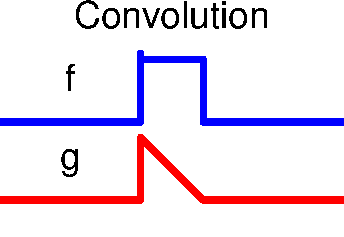
\includegraphics[page=1, width=\linewidth]{media/convolution1.pdf}
        \end{minipage}
        \hspace{.04\linewidth}
        \begin{minipage}[H]{.3\linewidth}
            \centering
            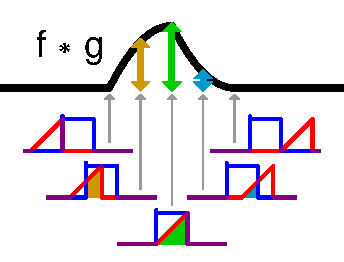
\includegraphics[page=1, width=\linewidth]{media/convolution2.pdf}
        \end{minipage}
        \caption{Example of a convolution of two functions \parenciteit{}{Convolution:Image}}
        \label{fig:ConvolutionExample}
    \end{figure} 
    \noindent This property is very useful when the differential calculations start to get complicated. To understand it better and also develop the discussion towards its connection with physics, let us try to solve, in the following Section, an example related to electrical engineering.
    
    \subsubsection{Electrical engineering \& Differential calculus \& Laplace} \label{sec:ElectronicsCalculusLaplace}
    Consider the circuit in the following Figure \ref{fig:CapTrasferFunctionExampleSchematic}:
    \begin{figure}[H]
        \centering
        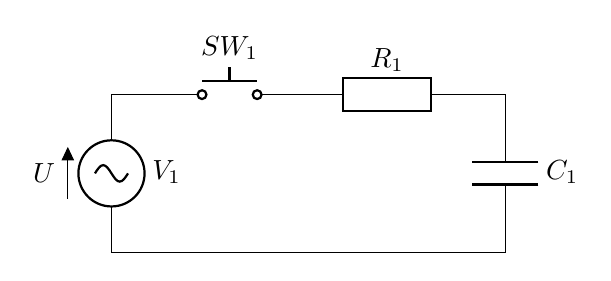
\begin{tikzpicture}[transform shape, use fpu reciprocal]
            \draw (0,-2)
                to[sV=$U$, l_=$V_1$] ++(0,2)
                -- ++(.5,0)
                to[nopb=$SW_1$] ++(2,0)
                to[R, l=$R_1$] ++(2,0)
                -- ++(.5,0)
                to[C, l=$C_1$] ++(0,-2)
                -- ++(-5,0);
        \end{tikzpicture}
        \caption{The circuit consisting of an alternating voltage source $V_1$ of $U[V]$, a capacitor $C_1$, a resistor $R_1$ and a switch $SW_1$}
        \label{fig:CapTrasferFunctionExampleSchematic}
    \end{figure}
    \noindent When the switch $SW_1$ is pressed, it closes the circuit and allows current to flow from the source $U_1$ through the capacitor $C_1$ and the resistor $R_1$.

    \noindent Let us try to describe the situation from a physical point of view to find the current $I$ of the circuit by means of differential calculus:
    \begin{figure}[H]
        \centering
        \begin{minipage}[b]{.21\linewidth}
            \centering
            \begin{equation} \label{eqn:CapTrasferFunctionExample1}
                U = A \cdot e^{j \left( \omega t + \phi \right)}
            \end{equation}
        \end{minipage}
        \hspace{0.04\linewidth}
        \begin{minipage}[b]{.21\linewidth}
            \centering
            \begin{equation} \label{eqn:CapTrasferFunctionExample2}
                \phi = 0
            \end{equation}
        \end{minipage}
        \hspace{0.04\linewidth}
        \begin{minipage}[b]{.21\linewidth}
            \centering
            \begin{equation} \label{eqn:CapTrasferFunctionExample3}
                Q = C \cdot U
            \end{equation}
        \end{minipage}
        \hspace{0.04\linewidth}
        \begin{minipage}[b]{.21\linewidth}
            \centering
            \begin{equation} \label{eqn:CapTrasferFunctionExample4}
                I = \frac{\textrm{d}Q}{\textrm{d}t}
            \end{equation}
        \end{minipage}
    \end{figure}

    \noindent So:
    \begin{itemize}
        \item (\ref{eqn:CapTrasferFunctionExample1}), gives us the voltage function followed by the source $V_1$, which is a
        phasor with its modulus stretched $A$ times \emph{(the amplitude)}, with frequency $\omega$ and phase shift $\phi$.
        \item (\ref{eqn:CapTrasferFunctionExample2}), tells us that the phase of the source's wave function does not matter to us, because if we vary the phase shift we can compensate for it with the time $t$ \emph{(In fact, at the end we will see that we find a function that does not depend on time)}.
        \item (\ref{eqn:CapTrasferFunctionExample3}), gives us the relation between the charge $Q$, the capacitance $C$ of the capacitor and its voltage, which corresponds to $U$.
        \item (\ref{eqn:CapTrasferFunctionExample4}), gives us another way of writing the current $I$ of the circuit.
    \end{itemize} 
    \begin{align}
        I &= C \cdot \frac{\textrm{d}U}{\textrm{d}t} \label{eqn:CapTrasferFunctionExample5} \\
        I &= C \cdot \frac{\textrm{d}e^{j \left( \omega t + \phi \right)}}{\textrm{d}t} \label{eqn:CapTrasferFunctionExample6} \\
        I &= C \cdot \frac{\textrm{d}e^{j \left( \omega t\right)}}{\textrm{d}t} \label{eqn:CapTrasferFunctionExample7} \\
        I &= C \cdot e^{j \left( \omega t \right)} \cdot j \omega \label{eqn:CapTrasferFunctionExample8} \\
        I &= C U j \omega \label{eqn:CapTrasferFunctionExample9}
    \end{align}
    \begin{itemize}
        \item (\ref{eqn:CapTrasferFunctionExample5}), we substitute equation (\ref{eqn:CapTrasferFunctionExample3}) for the charge $Q$ in equation (\ref{eqn:CapTrasferFunctionExample4}).
        \item (\ref{eqn:CapTrasferFunctionExample6}), we replace $U$ with the equivalence defined in (\ref{eqn:CapTrasferFunctionExample1}).
        \item (\ref{eqn:CapTrasferFunctionExample7}), we replace the phase shift $\phi$ with its value defined in (\ref{eqn:CapTrasferFunctionExample2}).
        \item (\ref{eqn:CapTrasferFunctionExample8}), is obtained by simplifying the derivative with respect to time $t$.
        \item (\ref{eqn:CapTrasferFunctionExample9}), the wave function is simplified to $U$ via the relation given in (\ref{eqn:CapTrasferFunctionExample1})\footnote{Note that the variable $t$ disappears completely}.
    \end{itemize}

    \noindent At this point we can try to find the "total resistance", or, put correctly, the total impedance $Z$\footnote{$Z$, the impedance, is the same as resistance $R$ (it is also measured in $[\Omega]$), and it is used when one wants to indicate a resistance with a complex value (this will be clarified later in this Section)} of the circuit:
    \begin{figure}[H]
        \centering
        \begin{minipage}[b]{.21\linewidth}
            \centering
            \begin{equation} \label{eqn:CapTrasferFunctionExample10}
                U = I \cdot Z
            \end{equation}
        \end{minipage}
        \hspace{0.04\linewidth}
        \begin{minipage}[b]{.21\linewidth}
            \centering
            \begin{equation} \label{eqn:CapTrasferFunctionExample11}
                I = C U j \omega
            \end{equation}
        \end{minipage}
        \hspace{0.04\linewidth}
        \begin{minipage}[b]{.21\linewidth}
            \centering
            \begin{equation} \label{eqn:CapTrasferFunctionExample12}
                s = j\omega + \sigma
            \end{equation}
        \end{minipage}
        \hspace{0.04\linewidth}
        \begin{minipage}[b]{.21\linewidth}
            \centering
            \begin{equation} \label{eqn:CapTrasferFunctionExample13}
                \sigma = 0
            \end{equation}
        \end{minipage}
    \end{figure}
    \begin{itemize}
        \item (\ref{eqn:CapTrasferFunctionExample10}), Ohm's law\footcite[]{Ohm:Wiki} with the complex impedance variable $Z$ in place of the real resistance $R$.
        \item (\ref{eqn:CapTrasferFunctionExample11}), reference to the equation obtained in the previous calculation (\ref{eqn:CapTrasferFunctionExample9}).
        \item (\ref{eqn:CapTrasferFunctionExample12}), definition of $s$ given in Section \ref{sec:MathAndPhysics}.
        \item (\ref{eqn:CapTrasferFunctionExample13}), assumption that $\sigma$, the signal growth coefficient, is equal to $0$.
    \end{itemize}
    \begin{align}
        Z &= \frac{U}{C U j \omega} \label{eqn:CapTrasferFunctionExample14} \\
        Z &= \frac{1}{C s} \label{eqn:CapTrasferFunctionExample15}
    \end{align}
    \begin{itemize}
        \item (\ref{eqn:CapTrasferFunctionExample14}), is obtained by substituting (\ref{eqn:CapTrasferFunctionExample11}) for $I$ in Ohm's law (\ref{eqn:CapTrasferFunctionExample10}).
        \item (\ref{eqn:CapTrasferFunctionExample15}), simplification of the equation using the definition of $s$ in (\ref{eqn:CapTrasferFunctionExample12}).
    \end{itemize}
    \noindent Exactly at this point in the procedure we notice that $Z$ is defined by a constant\footnote{An ideal capacitor does not change its capacitance value} $C$ and the variable $s$.
    Consequently we can write the following function:
    \begin{equation} \label{eqn:CapTrasferFunctionExample16}
        Z(s) = \frac{1}{C s}
    \end{equation}

    \noindent The fact that $Z(s)$ is a function with complex values allows us to separate impedance values into the parts corresponding to "classic" direct-current resistances, through the real components, and to alternating-current resistances, through the imaginary components.

    The differential calculation we have just solved to find $Z(s)$ can also be done for the other passive components\footnote{Passive components are considered to be resistors $R$, inductors $L$ and capacitors $C$} to obtain:
    \begin{figure}[H]
        \centering
        \begin{minipage}[b]{.3\linewidth}
            \centering
            \begin{equation*}
                Z_R(s)=R
            \end{equation*}
        \end{minipage}
        \hspace{0.04\linewidth}
        \begin{minipage}[b]{.3\linewidth}
            \centering
            \begin{equation*}
                Z_C(s) = \frac{1}{C s}
            \end{equation*}
        \end{minipage}
        \hspace*{0.04\linewidth}
        \begin{minipage}[b]{.3\linewidth}
            \centering
            \begin{equation*}
                Z_L(s) = {L s}
            \end{equation*}
        \end{minipage}
    \end{figure}
    
    Even intuitively one can understand that the capacitor's impedance function gives ever smaller values as frequency increases.
    This characteristic of the capacitor might suggest the idea of using this property to our advantage, namely to attenuate some frequencies more than others.
    In this way we arrive at understanding the concept of how analog frequency filters work.

    Allow me to slightly modify the variable names and the circuit to turn it into a true frequency filter:
    \begin{figure}[H]
        \centering
        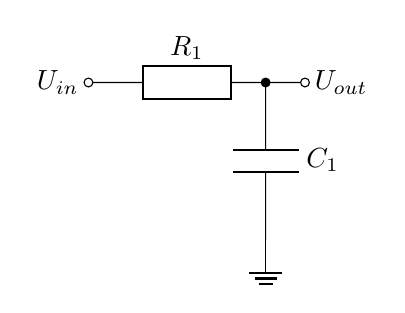
\begin{tikzpicture}[transform shape, use fpu reciprocal]
            \draw (0,0)
                node[left]{$U_{in}$}
                to[short, o-] ++(.25,0)
                to[R, -*, l=$R_1$] ++(2,0)
                coordinate(joint)
                to[short, -o] ++(.5,0)
                node[right]{$U_{out}$}
                (joint) to[C, l=$C_1$] ++(0,-2)
                node[ground]{} ++(0,0);
        \end{tikzpicture}
        \caption{First-order LPF \emph{(Low Pass Filter, which attenuates the high frequencies of the signal)} with input signal $U_{in}$ and output signal $U_{out}$; the other parts remain the same as in Figure \ref{fig:CapTrasferFunctionExampleSchematic}}
        \label{fig:CapFilterExample}
    \end{figure}

    \noindent Now let us try to derive the transfer function of the filter using the impedance function we have just found:
    \begin{figure}[H]
        \centering
        \begin{minipage}[b]{.3\linewidth}
            \centering
            \begin{equation} \label{eqn:CapTrasferFunctionExample17}
                H(s) = \frac{U_{out}}{U_{in}}
            \end{equation}
        \end{minipage}
        \hspace{0.04\linewidth}
        \begin{minipage}[b]{.3\linewidth}
            \centering
            \begin{equation} \label{eqn:CapTrasferFunctionExample18}
                Z(s) = \frac{1}{C s}
            \end{equation}
        \end{minipage}
        \hspace*{0.04\linewidth}
        \begin{minipage}[b]{.3\linewidth}
            \centering
            \begin{equation} \label{eqn:CapTrasferFunctionExample19}
                U_{out} = U_{in} \cdot \frac{Z_b}{Z_a + Z_b}
            \end{equation}
        \end{minipage}
    \end{figure}
    \begin{itemize}
        \item (\ref{eqn:CapTrasferFunctionExample17}), one of the ways to define a transfer function, mentioned in Section \ref{sec:MathAndPhysics}.
        \item (\ref{eqn:CapTrasferFunctionExample18}), the capacitor impedance function just calculated (\ref{eqn:CapTrasferFunctionExample16}).
        \item (\ref{eqn:CapTrasferFunctionExample19}), formula derived from Ohm's and Kirchhoff's laws\footcite[]{Kirchhoff:Wiki} that allows us to calculate the voltage at the point $U_{out}$ knowing the values of the resistances and the input voltage $U_{in}$.
    \end{itemize}
    \begin{align}
        U_{out} &= U_{in} \cdot \frac{\frac{1}{C s}}{\frac{1}{C s}+R} \label{eqn:CapTrasferFunctionExample20} \\
        \frac{U_{out}}{U_{in}} &= \frac{\frac{1}{C s}}{\frac{1}{C s}+R} \label{eqn:CapTrasferFunctionExample21} \\
        H(s) &= \frac{\frac{1}{C s}}{\frac{1}{C s}+R} \label{eqn:CapTrasferFunctionExample22} \\
        H(s) &= \frac{1}{R C s + 1} \label{eqn:CapTrasferFunctionExample23}
    \end{align}
    \begin{itemize}
        \item (\ref{eqn:CapTrasferFunctionExample20}), substitution of the values of $R_1$ and $C_1$ \emph{(the impedance $Z$ (\ref{eqn:CapTrasferFunctionExample18}))} into (\ref{eqn:CapTrasferFunctionExample19}) \emph{(of course replacing the names of the first impedance $Z_a$ with $R$ and of the second $Z_b$ with $Z(s)$)}.
        \item (\ref{eqn:CapTrasferFunctionExample21}), division of both sides of the equation by $U_{in}$.
        \item (\ref{eqn:CapTrasferFunctionExample22}), substitution of $\frac{U_{out}}{U_{in}}$ with (\ref{eqn:CapTrasferFunctionExample17}).
        \item (\ref{eqn:CapTrasferFunctionExample23}), multiplication of the numerator and denominator of the fraction by $C s$.
    \end{itemize}
    \noindent The function we have found has the characteristic form of a transfer function already seen in Section \ref{sec:TransformsAndLaplace}, which in this case is only first-order.
    Moreover, what I already mentioned earlier\footnote{Section \ref{sec:TransformsAndLaplace}} holds: the calculations are quite numerous for a truly simple circuit.
    This is where the Laplace transform comes to the rescue\footnote{Its greatest potential shows when circuits become networks of passive components that are very difficult to describe with differential calculus and then simplify to make them usable}.

    \noindent Let us try to make the filter more complex by chaining copies of it at the input:
    \begin{figure}[H]
        \centering
        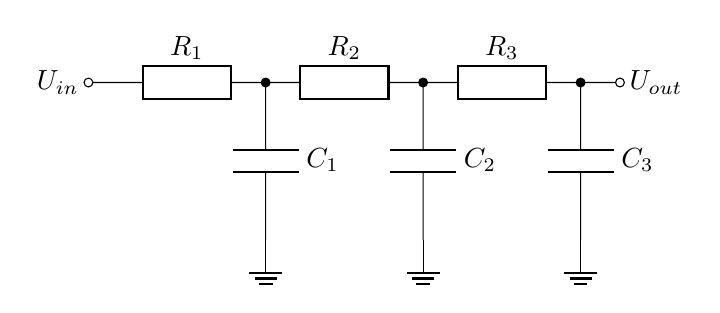
\begin{tikzpicture}[transform shape, use fpu reciprocal]
            \draw (0,0)
                node[left]{$U_{in}$}
                to[short, o-] ++(.25,0)
                to[R, -*, l=$R_1$] ++(2,0)
                coordinate(joint)
                to[C, l=$C_1$] ++(0,-2)
                node[ground]{} ++(0,-.15)
                (joint) to[R, -*, l=$R_2$] ++(2,0)
                coordinate(joint1)
                to[C, l=$C_2$] ++(0,-2)
                node[ground]{} ++(0,-.15)
                (joint1) to[R, -*, l=$R_3$] ++(2,0)
                coordinate(joint2)
                to[C, l=$C_3$] ++(0,-2)
                node[ground]{} ++(0,0)
                (joint2) to[short, -o] ++(.5,0)
                node[right]{$U_{out}$};
        \end{tikzpicture}
        \caption{Third-order LPF with input signal $U_{in}$, output signal $U_{out}$, and passive components \emph{($R_x$, $C_x$)} obtained by chaining copies of the filter in Figure \ref{fig:CapFilterExample}}
        \label{fig:CapFilterExample2}
    \end{figure}
    \noindent In this example, since we made copies of the filter from the previous example\footnote{\ref{fig:CapFilterExample}}, we set the following condition:
    \begin{figure}[H]
        \centering
        \begin{minipage}[b]{.31\linewidth}
            \centering
            \begin{equation*}
                R = R_1 = R_2 = R_3
            \end{equation*}
        \end{minipage}
        \hspace{0.04\linewidth}
        \begin{minipage}[b]{.31\linewidth}
            \centering
            \begin{equation*}
                C = C_1 = C_2 = C_3
            \end{equation*}
        \end{minipage}
    \end{figure}
    \noindent To find the system response $U_{out}$ to a signal $U_{in}$, instead of describing the circuit with differential calculus it suffices to compose the following expression:
    \begin{equation*}
        H_{LPF\_III}(s) = \frac{1}{RCs+1} \cdot \frac{1}{RCs+1} \cdot \frac{1}{RCs+1} = \frac{1}{\left(RCs+1\right)^3}
    \end{equation*}
    \noindent Then the inverse Laplace transform of the transfer function just obtained is taken:
    \begin{equation*}
        \mathcal{L}^{-1}\{H_{LPF\_III}\}(t) = \int_{c-j\infty}^{c+j\infty} e^{f_{LPF\_III}t} H_{LPF\_III}(s) \mathrm{d}s
    \end{equation*}
    \noindent The inverse transform is harder to compute than the transform itself, but there are tables of precomputed expressions, similar in concept to the rules of differentiation.
    Moreover, for convenience and to avoid making mistakes, I use a programming language called Maple\footcite[]{Maplesoft:Software}, which can manipulate mathematical expressions in symbolic form\footnote{Python, R, Matlab are programming languages well known for their ease of use for mathematical calculations, which unfortunately cannot handle calculations with undeclared parameters} and which comes with its own software environment for convenience.
    So, using Maple we obtain:
    \begin{equation*}
        \mathcal{L}^{-1}\{H_{LPF\_III}\}(t) = f_{LPF\_III}(t) = t^2 \cdot \frac{e^{-\frac{t}{RC}}}{2RC^3}
    \end{equation*}
    As a check of the correctness of the result obtained, we can note that the function is a harmonic function.

    At this point we can move the discussion from Laplace transforms towards electrical engineering with the knowledge available.

    \subsubsection{Types of frequency filters}
    To work graphically with transfer functions in the frequency domain we must first convert them in a certain way, because initially their values are complex numbers.
    To obtain the factor by which the transfer functions amplify the signal we must take the modulus of the transfer function, while to obtain the phase shift we need to take the argument of the function:
    \begin{figure}[H]
        \centering
        \begin{minipage}[b]{.31\linewidth}
            \centering
            \begin{equation*}
                A = \left|H(s)\right|
            \end{equation*}
        \end{minipage}
        \hspace{0.04\linewidth}
        \begin{minipage}[b]{.31\linewidth}
            \centering
            \begin{equation*}
                \theta = \angle\left(H(s)\right)
            \end{equation*}
        \end{minipage}
    \end{figure}
    \noindent Knowing this, we can study them.

    To simplify the concepts I divide filter transfer functions into simple and complex ones: the simple ones are the transfer functions that can be combined in different ways to vary the resulting complex function.
    
    \noindent See the following plots \ref{fig:SimpleBodeExample} and \ref{fig:ComplicateBodeExample}:
    \begin{figure}[H]
        \centering
        \begin{minipage}[H]{.45\linewidth}
            \centering
            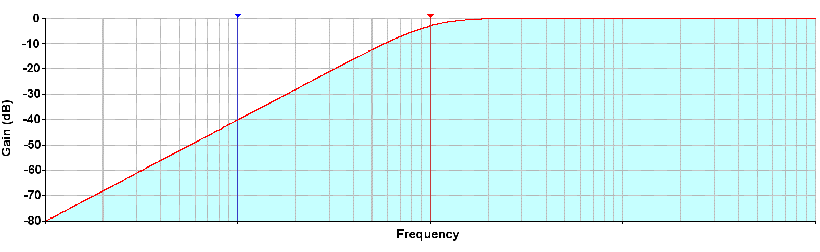
\includegraphics[width=\linewidth]{media/sloa093_HPF.pdf}
            \subcaption{}
            \label{fig:SimpleBodeExampleHPF}
        \end{minipage}
        \hspace{.04\linewidth}
        \begin{minipage}[H]{.45\linewidth}
            \centering
            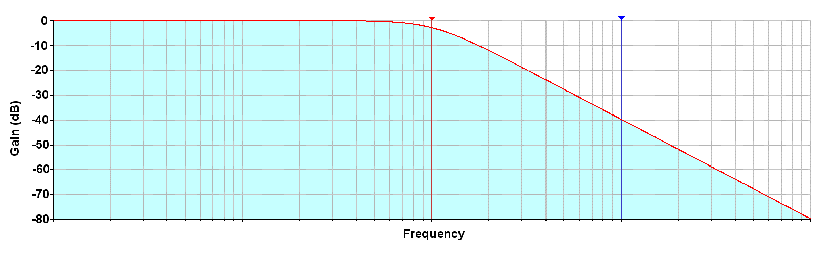
\includegraphics[width=\linewidth]{media/sloa093_LPF.pdf}
            \subcaption{}
            \label{fig:SimpleBodeExampleLPF}
        \end{minipage}
        \caption{Example of the gain response in the frequency domain of simple transfer functions: \ref{fig:SimpleBodeExampleHPF} High-Pass or HPF, which attenuates low frequencies, \ref{fig:SimpleBodeExampleLPF} Low-Pass or LPF, which attenuates high frequencies \emph{(the "F" in the abbreviations stands for Filter) \parenciteit{}{FilterPassStopTypes:Image}}}
        \label{fig:SimpleBodeExample}
    \end{figure}
    \noindent The complex functions, instead, are:
    \begin{figure}[H]
        \centering
        \begin{minipage}[H]{.45\linewidth}
            \centering
            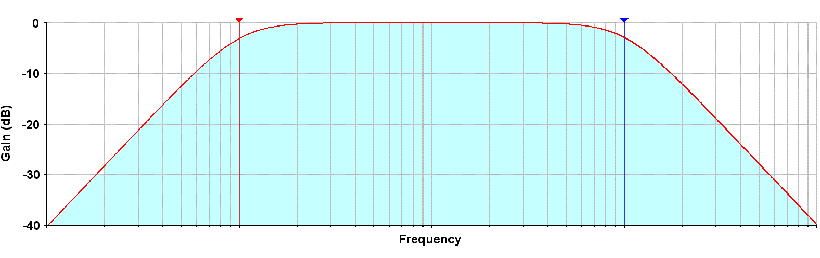
\includegraphics[width=\linewidth]{media/sloa093_BPF.pdf}
            \subcaption{}
            \label{fig:ComplicateBodeExampleBPF}
        \end{minipage}
        \hspace{.04\linewidth}
        \begin{minipage}[H]{.45\linewidth}
            \centering
            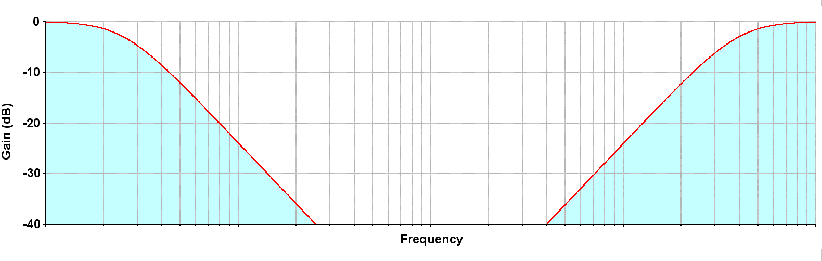
\includegraphics[width=\linewidth]{media/sloa093_BSF.pdf}
            \subcaption{}
            \label{fig:ComplicateBodeExampleBSF}
        \end{minipage}
        \\
        \begin{minipage}[H]{.45\linewidth}
            \centering
            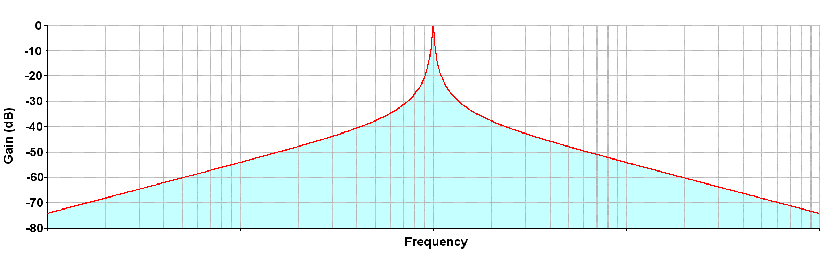
\includegraphics[width=\linewidth]{media/sloa093_NPF.pdf}
            \subcaption{}
            \label{fig:ComplicateBodeExampleNPF}
        \end{minipage}
        \hspace{.04\linewidth}
        \begin{minipage}[H]{.45\linewidth}
            \centering
            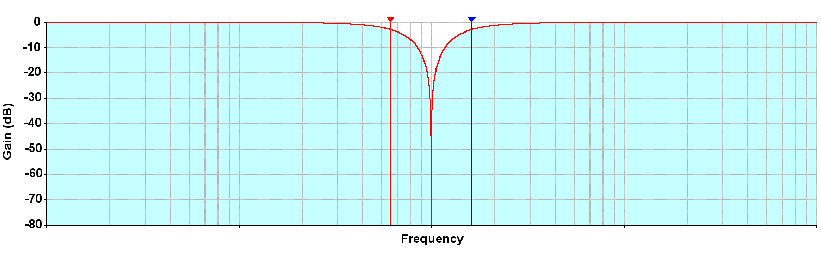
\includegraphics[width=\linewidth]{media/sloa093_NSF.pdf}
            \subcaption{}
            \label{fig:ComplicateBodeExampleNSF}
        \end{minipage}
        \caption{Example of the gain response in the frequency domain of complex transfer functions: \ref{fig:ComplicateBodeExampleBPF} Band-Pass or BPF, which passes a band of frequencies, \ref{fig:ComplicateBodeExampleBSF} Band-Rejection or BRF, which attenuates a band of frequencies, \ref{fig:ComplicateBodeExampleNPF} Narrow-Band-Pass or NPF, which passes a narrow band of frequencies, \ref{fig:ComplicateBodeExampleNSF} Narrow-Band-Rejection or NRF, which attenuates a narrow band of frequencies \parenciteit{}{FilterPassStopTypes:Image}}
        \label{fig:ComplicateBodeExample}
    \end{figure}
    \clearpage

    \noindent Variations of the filter order and of the parameter $\sigma$ manifest themselves in the frequency domain as follows, as in Figure \ref{fig:FunctionShapesOrder}:
    \begin{figure}[H]
        \centering
        \begin{minipage}[H]{.45\linewidth}
            \centering
            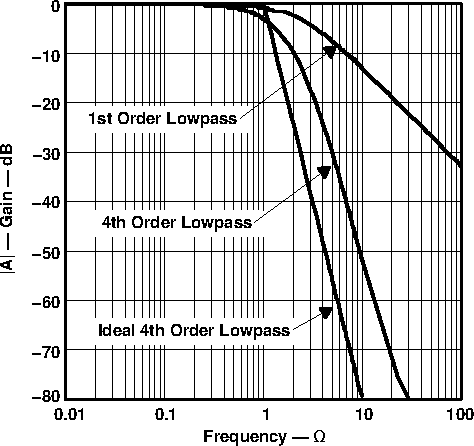
\includegraphics[width=\linewidth]{media/sloa088_order.pdf}
            \label{fig:FunctionOrder}
            \subcaption{Transfer functions of different shapes resulting from varying their order}
        \end{minipage}
        \hspace{.04\linewidth}
        \begin{minipage}[H]{.45\linewidth}
            \centering
            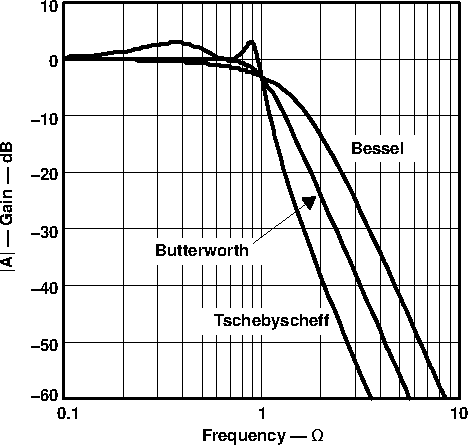
\includegraphics[width=\linewidth]{media/sloa088_shape.pdf}
            \label{fig:FunctionShapes}
            \subcaption{Transfer functions of different shapes resulting from varying $\sigma$}
        \end{minipage}
        \caption{Example of the gain response in the frequency domain of normalized low-pass transfer functions \emph{($\Omega$ denotes the normalized frequency, i.e. the cutoff frequency of the function has been moved to the value $1$)} \parenciteit{}{SLOA088}}
        \label{fig:FunctionShapesOrder}
    \end{figure}
    % TRANSLATOR NOTE: original "puo al massimo contenerne una" ("can contain at most one") has no clear referent; rendered as "can contribute at most one order".
    \noindent The order of an analog filter can only be changed by adding components to the impedance network\footnote{This can be deduced from the knowledge given in Section \ref{sec:ElectronicsCalculusLaplace}}, because a passive electrical element can contribute at most one order.
    The shape of the function, instead, is a trade-off between the steepness of the frequency cutoff and how flat the response is in the part of the function that must remain intact.

    In my project the phase shift of the transfer function is irrelevant\footnote{I believe that the artificial intelligence that will process the received information in future iterations of the project is not affected by the phase shift of the signal: it is enough that the function is identical on all sensor boards}, which is why I allow myself to skip describing the characteristics of the different function shapes.
    Instead I present a single shape: Butterworth\footnote{Shown in Figure \ref{fig:FunctionShapesOrder}}, the most effective in terms of how flat the part of the function that must remain intact is and how quickly it is cut off at the required frequency\footnote{Concept taken from the explanation in \parenciteit{p6}{SLOA088}}.
    Butterworth has a cutoff steepness\footnote{Also called the rolloff rate} of 20dB/dec\footnote{The unit indicates how much the filter gain decreases when the frequency changes by a factor of ten} per order\footnote{The rolloff of a given order can be found by multiplying the filter order by the rolloff of the first order}.

    To better see how transfer functions form as the parameter $\sigma$ varies, I decided to put it on one of the coordinate axes and obtained the following plots in Figure \ref{fig:3DFUNCExample}:
    \begin{figure}[H]
        \centering
        \begin{minipage}[H]{.45\linewidth}
            \centering
            \newcommand{\plotDir}{datasets/s_plot_example_data}
            \newcommand{\plotName}{hpf_2}
            \import{\plotDir}{\plotName_def.tex}%
            \begin{tikzpicture}
                \begin{axis}[
                    width=\linewidth,
                    view = {20}{30},
                    % ymode=log,
                    xmin = \minX,
                    xmax = \maxX,
                    ymin = \minY,
                    ymax = \maxY,
                    zmin = \minZ,
                    zmax = \maxZ,
                    xtick = {\minTickX,\nextTickX,...,\maxTickX},
                    ytick = {\minTickY,\nextTickY,...,\maxTickY},
                    ztick = {\minTickZ,\nextTickZ,...,\maxTickZ},
                    xlabel={\legendX},
                    ylabel={\legendY},
                    zlabel={\legendZ},
                    label style={font=\footnotesize},
                    tick label style={font=\tiny},
                    smooth,
                    grid = both,
                    ymajorgrids = true,
                    line join=round,
                    clip=false
                ]
                \addplot3[
                    surf,
                    /pgfplots/colormap={bone}{rgb255=(0,0,0) rgb255=(84,84,116) rgb255=(167,199,199) rgb255=(240,240,240)},
                    opacity=0.9375,
                    shader=faceted interp,
                    patch type=coons,
                    z buffer=sort,
                    patch table=\plotDir/\plotName_anchors.csv
                ] table [col sep=comma,header=false] {\plotDir/\plotName.csv};
                \end{axis}
            \end{tikzpicture}
            \import{\plotDir}{All_plots_undef.tex}%
            \let\plotDir\undefined
            \let\plotName\undefined
            \subcaption{}
            \label{fig:HPF2Example}
        \end{minipage}
        \hspace{.04\linewidth}
        \begin{minipage}[H]{.45\linewidth}
            \centering
            \newcommand{\plotDir}{datasets/s_plot_example_data}
            \newcommand{\plotName}{lpf_2}
            \import{\plotDir}{\plotName_def.tex}%
            \begin{tikzpicture}
                \begin{axis}[
                    width=\linewidth,
                    view = {20}{30},
                    % ymode=log,
                    xmin = \minX,
                    xmax = \maxX,
                    ymin = \minY,
                    ymax = \maxY,
                    zmin = \minZ,
                    zmax = \maxZ,
                    xtick = {\minTickX,\nextTickX,...,\maxTickX},
                    ytick = {\minTickY,\nextTickY,...,\maxTickY},
                    ztick = {\minTickZ,\nextTickZ,...,\maxTickZ},
                    xlabel={\legendX},
                    ylabel={\legendY},
                    zlabel={\legendZ},
                    label style={font=\footnotesize},
                    tick label style={font=\tiny},
                    smooth,
                    grid = both,
                    ymajorgrids = true,
                    line join=round,
                    clip=false
                ]
                \addplot3[
                    surf,
                    /pgfplots/colormap={bone}{rgb255=(0,0,0) rgb255=(84,84,116) rgb255=(167,199,199) rgb255=(240,240,240)},
                    opacity=0.9375,
                    shader=faceted interp,
                    patch type=coons,
                    z buffer=sort,
                    patch table=\plotDir/\plotName_anchors.csv
                ] table [col sep=comma,header=false] {\plotDir/\plotName.csv};
                \end{axis}
            \end{tikzpicture}
            \import{\plotDir}{All_plots_undef.tex}%
            \let\plotDir\undefined
            \let\plotName\undefined
            \subcaption{}
            \label{fig:LPF2Example}
        \end{minipage}
        \\
        \begin{minipage}[H]{.45\linewidth}
            \centering
            \newcommand{\plotDir}{datasets/s_plot_example_data}
            \newcommand{\plotName}{bpf_2}
            \import{\plotDir}{\plotName_def.tex}%
            \begin{tikzpicture}
                \begin{axis}[
                    width=\linewidth,
                    view = {20}{30},
                    % ymode=log,
                    xmin = \minX,
                    xmax = \maxX,
                    ymin = \minY,
                    ymax = \maxY,
                    zmin = \minZ,
                    zmax = \maxZ,
                    xtick = {\minTickX,\nextTickX,...,\maxTickX},
                    ytick = {\minTickY,\nextTickY,...,\maxTickY},
                    ztick = {\minTickZ,\nextTickZ,...,\maxTickZ},
                    xlabel={\legendX},
                    ylabel={\legendY},
                    zlabel={\legendZ},
                    label style={font=\footnotesize},
                    tick label style={font=\tiny},
                    smooth,
                    grid = both,
                    ymajorgrids = true,
                    line join=round,
                    clip=false
                ]
                \addplot3[
                    surf,
                    /pgfplots/colormap={bone}{rgb255=(0,0,0) rgb255=(84,84,116) rgb255=(167,199,199) rgb255=(240,240,240)},
                    opacity=0.9375,
                    shader=faceted interp,
                    patch type=coons,
                    z buffer=sort,
                    patch table=\plotDir/\plotName_anchors.csv
                ] table [col sep=comma,header=false] {\plotDir/\plotName.csv};
                \end{axis}
            \end{tikzpicture}
            \import{\plotDir}{All_plots_undef.tex}%
            \let\plotDir\undefined
            \let\plotName\undefined
            \subcaption{}
            \label{fig:BPF2Example}
        \end{minipage}
        \hspace{.04\linewidth}
        \begin{minipage}[H]{.45\linewidth}
            \centering
            \newcommand{\plotDir}{datasets/s_plot_example_data}
            \newcommand{\plotName}{bpf_4}
            \import{\plotDir}{\plotName_def.tex}%
            \begin{tikzpicture}
                \begin{axis}[
                    width=\linewidth,
                    view = {20}{30},
                    % ymode=log,
                    xmin = \minX,
                    xmax = \maxX,
                    ymin = \minY,
                    ymax = \maxY,
                    zmin = \minZ,
                    zmax = \maxZ,
                    xtick = {\minTickX,\nextTickX,...,\maxTickX},
                    ytick = {\minTickY,\nextTickY,...,\maxTickY},
                    ztick = {\minTickZ,\nextTickZ,...,\maxTickZ},
                    xlabel={\legendX},
                    ylabel={\legendY},
                    zlabel={\legendZ},
                    label style={font=\footnotesize},
                    tick label style={font=\tiny},
                    smooth,
                    grid = both,
                    ymajorgrids = true,
                    line join=round,
                    clip=false
                ]
                \addplot3[
                    surf,
                    /pgfplots/colormap={bone}{rgb255=(0,0,0) rgb255=(84,84,116) rgb255=(167,199,199) rgb255=(240,240,240)},
                    opacity=0.9375,
                    shader=faceted interp,
                    patch type=coons,
                    z buffer=sort,
                    patch table=\plotDir/\plotName_anchors.csv
                ] table [col sep=comma,header=false] {\plotDir/\plotName.csv};
                \end{axis}
            \end{tikzpicture}
            \import{\plotDir}{All_plots_undef.tex}%
            \let\plotDir\undefined
            \let\plotName\undefined
            \subcaption{}
            \label{fig:BPF4Example}
        \end{minipage}
        \begin{minipage}[H]{.45\linewidth}
            \centering
            \newcommand{\plotDir}{datasets/s_plot_log_example_data}
            \newcommand{\plotName}{hpf_2}
            \import{\plotDir}{\plotName_def.tex}%
            \begin{tikzpicture}
                \begin{axis}[
                    width=\linewidth,
                    view = {70}{30},
                    ymode=log,
                    log ticks with fixed point,
                    xmin = \minX,
                    xmax = \maxX,
                    ymin = \minY,
                    ymax = \maxY,
                    zmin = \minZ,
                    zmax = \maxZ,
                    xtick = {\minTickX,\nextTickX,...,\maxTickX},
                    ytick = {\minTickY,\nextTickY,...,\maxTickY},
                    ztick = {\minTickZ,\nextTickZ,...,\maxTickZ},
                    xlabel={\legendX},
                    ylabel={\legendY},
                    zlabel={\legendZ},
                    label style={font=\footnotesize},
                    tick label style={font=\tiny},
                    smooth,
                    grid = both,
                    ymajorgrids = true,
                    line join=round,
                    clip=false,
                    y tick label style = {rotate=-60, anchor=west}
                ]
                \addplot3[
                    surf,
                    /pgfplots/colormap={bone}{rgb255=(0,0,0) rgb255=(84,84,116) rgb255=(167,199,199) rgb255=(240,240,240)},
                    opacity=0.9375,
                    shader=faceted interp,
                    patch type=coons,
                    z buffer=sort,
                    patch table=\plotDir/\plotName_anchors.csv
                ] table [col sep=comma,header=false] {\plotDir/\plotName.csv};
                \end{axis}
            \end{tikzpicture}
            \import{\plotDir}{All_plots_undef.tex}%
            \let\plotDir\undefined
            \let\plotName\undefined
            \subcaption{}
            \label{fig:HPF2logExample}
        \end{minipage}
        \hspace{.04\linewidth}
        \begin{minipage}[H]{.45\linewidth}
            \centering
            \newcommand{\plotDir}{datasets/s_plot_log_example_data}
            \newcommand{\plotName}{lpf_2}
            \import{\plotDir}{\plotName_def.tex}%
            \begin{tikzpicture}
                \begin{axis}[
                    width=\linewidth,
                    view = {70}{30},
                    ymode=log,
                    log ticks with fixed point,
                    xmin = \minX,
                    xmax = \maxX,
                    ymin = \minY,
                    ymax = \maxY,
                    zmin = \minZ,
                    zmax = \maxZ,
                    xtick = {\minTickX,\nextTickX,...,\maxTickX},
                    ytick = {\minTickY,\nextTickY,...,\maxTickY},
                    ztick = {\minTickZ,\nextTickZ,...,\maxTickZ},
                    xlabel={\legendX},
                    ylabel={\legendY},
                    zlabel={\legendZ},
                    label style={font=\footnotesize},
                    tick label style={font=\tiny},
                    smooth,
                    grid = both,
                    ymajorgrids = true,
                    line join=round,
                    clip=false,
                    y tick label style = {rotate=-60, anchor=west}
                ]
                \addplot3[
                    surf,
                    /pgfplots/colormap={bone}{rgb255=(0,0,0) rgb255=(84,84,116) rgb255=(167,199,199) rgb255=(240,240,240)},
                    opacity=0.9375,
                    shader=faceted interp,
                    patch type=coons,
                    z buffer=sort,
                    patch table=\plotDir/\plotName_anchors.csv
                ] table [col sep=comma,header=false] {\plotDir/\plotName.csv};
                \end{axis}
            \end{tikzpicture}
            \import{\plotDir}{All_plots_undef.tex}%
            \let\plotDir\undefined
            \let\plotName\undefined
            \subcaption{}
            \label{fig:LPF2logExample}
        \end{minipage}
        \\
        \begin{minipage}[H]{.45\linewidth}
            \centering
            \newcommand{\plotDir}{datasets/s_plot_log_example_data}
            \newcommand{\plotName}{bpf_2}
            \import{\plotDir}{\plotName_def.tex}%
            \begin{tikzpicture}
                \begin{axis}[
                    width=\linewidth,
                    view = {70}{30},
                    ymode=log,
                    log ticks with fixed point,
                    xmin = \minX,
                    xmax = \maxX,
                    ymin = \minY,
                    ymax = \maxY,
                    zmin = \minZ,
                    zmax = \maxZ,
                    xtick = {\minTickX,\nextTickX,...,\maxTickX},
                    ytick = {\minTickY,\nextTickY,...,\maxTickY},
                    ztick = {\minTickZ,\nextTickZ,...,\maxTickZ},
                    xlabel={\legendX},
                    ylabel={\legendY},
                    zlabel={\legendZ},
                    label style={font=\footnotesize},
                    tick label style={font=\tiny},
                    smooth,
                    grid = both,
                    ymajorgrids = true,
                    line join=round,
                    clip=false,
                    y tick label style = {rotate=-60, anchor=west}
                ]
                \addplot3[
                    surf,
                    /pgfplots/colormap={bone}{rgb255=(0,0,0) rgb255=(84,84,116) rgb255=(167,199,199) rgb255=(240,240,240)},
                    opacity=0.9375,
                    shader=faceted interp,
                    patch type=coons,
                    z buffer=sort,
                    patch table=\plotDir/\plotName_anchors.csv
                ] table [col sep=comma,header=false] {\plotDir/\plotName.csv};
                \end{axis}
            \end{tikzpicture}
            \import{\plotDir}{All_plots_undef.tex}%
            \let\plotDir\undefined
            \let\plotName\undefined
            \subcaption{}
            \label{fig:BPF2logExample}
        \end{minipage}
        \hspace{.04\linewidth}
        \begin{minipage}[H]{.45\linewidth}
            \centering
            \newcommand{\plotDir}{datasets/s_plot_log_example_data}
            \newcommand{\plotName}{bpf_4}
            \import{\plotDir}{\plotName_def.tex}%
            \begin{tikzpicture}
                \begin{axis}[
                    width=\linewidth,
                    view = {70}{30},
                    ymode=log,
                    log ticks with fixed point,
                    xmin = \minX,
                    xmax = \maxX,
                    ymin = \minY,
                    ymax = \maxY,
                    zmin = \minZ,
                    zmax = \maxZ,
                    xtick = {\minTickX,\nextTickX,...,\maxTickX},
                    ytick = {\minTickY,\nextTickY,...,\maxTickY},
                    ztick = {\minTickZ,\nextTickZ,...,\maxTickZ},
                    xlabel={\legendX},
                    ylabel={\legendY},
                    zlabel={\legendZ},
                    label style={font=\footnotesize},
                    tick label style={font=\tiny},
                    smooth,
                    grid = both,
                    ymajorgrids = true,
                    line join=round,
                    clip=false,
                    y tick label style = {rotate=-60, anchor=west}
                ]
                \addplot3[
                    surf,
                    /pgfplots/colormap={bone}{rgb255=(0,0,0) rgb255=(84,84,116) rgb255=(167,199,199) rgb255=(240,240,240)},
                    opacity=0.9375,
                    shader=faceted interp,
                    patch type=coons,
                    z buffer=sort,
                    patch table=\plotDir/\plotName_anchors.csv
                ] table [col sep=comma,header=false] {\plotDir/\plotName.csv};
                \end{axis}
            \end{tikzpicture}
            \import{\plotDir}{All_plots_undef.tex}%
            \let\plotDir\undefined
            \let\plotName\undefined
            \subcaption{}
            \label{fig:BPF4logExample}
        \end{minipage}
        \caption{Four transfer functions of different types and orders with the gain axis on a logarithmic scale, with the frequency axis $\omega$ on a linear scale in \ref{fig:HPF2Example} \ref{fig:LPF2Example} \ref{fig:BPF2Example} \ref{fig:BPF4Example} and on a logarithmic scale \ref{fig:HPF2logExample} \ref{fig:LPF2logExample} \ref{fig:BPF2logExample} \ref{fig:BPF4logExample}}
        \label{fig:3DFUNCExample}
    \end{figure}
    \clearpage

    \subsubsection{Electrical engineering \& Filters}
    The filters we saw in Section \ref{sec:ElectronicsCalculusLaplace} in Figures \ref{fig:CapFilterExample} and \ref{fig:CapFilterExample2} increase the output resistance, and the only thing they do is attenuate the signal\footnote{In the real world, reading a voltage from a conductor requires some current to flow, and because of the filter's impedance (even for the frequencies that should not be attenuated) the voltage decreases}.
    Consequently we must amplify the signal to increase the order of the filter.
    The first idea that comes to mind is to put an operational amplifier, or OA, in series with the filter, but this choice is not the best, because there are active filters, i.e. filters that include an amplifier in their topology.
    The simplest and most popular are SK, or Sallen-Key, and MFB, or Multiple-Feedback Filter, which can be seen in the following Figure \ref{fig:SKMFBSchematic}
    \begin{figure}[H]
        \centering
        \begin{minipage}[H]{.45\linewidth}
            \centering
            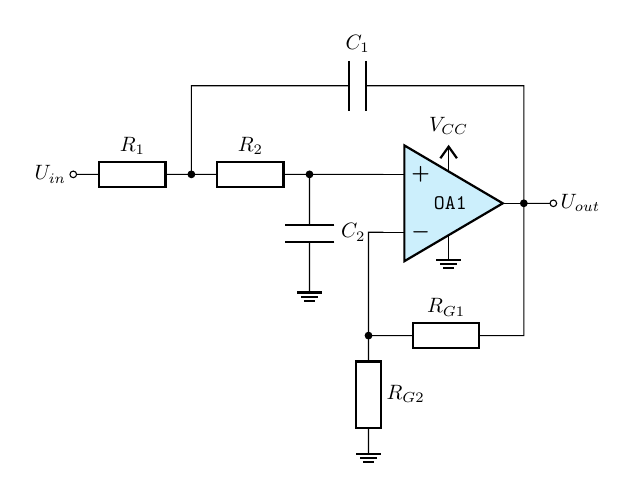
\begin{tikzpicture}[transform shape, use fpu reciprocal, scale=.75]
                \draw (0,0)
                    to[R, l=$R_1$, -*] ++(2,0)
                    coordinate(C1)
    
                    to[R, l=$R_2$, -*] ++(2,0)
                    coordinate(C2)
    
                    (C2)
                    -- ++(1.25,0)
                    node[op amp, noinv input up, fill=cyan!20, anchor=+](OA1){\texttt{OA1}}
    
                    (C2)
                    to[C, l=$C_2$] ++(0,-2)
                    node[tlground]{}
    
                    (OA1.-)
                    -- ++ (-.25,0)
                    -- ++(0,-1.75)
                    coordinate(Rg1Rg2)
                    to[R, l=$R_{G1}$, *-] (Rg1Rg2-|OA1.out)
                    to[short, -*] (OA1.out)
    
                    (Rg1Rg2) to[R, l=$R_{G2}$] ++(0,-2)
                    node[tlground]{}
    
                    (C1)
                    -- ++(0,1.5)
                    coordinate(R1start)
                    to[C, l=$C_1$] (R1start-|OA1.out)
                    -- (OA1.out)
    
                    (OA1.up)
                    node[vcc]{$V_{CC}$}
    
                    (OA1.down)
                    node[ground]{}
    
                    (OA1.out) ++(.5,0)
                    node[right]{$U_{out}$}
                    to[short, o-] ++(-.5,0)
    
                    (0,0)
                    node[left]{$U_{in}$}
                    to[short, o-] ++(0,0)
                    ;
            \end{tikzpicture}
            \subcaption{Sallen-Key topology; its advantage is that the values of $\sigma$ and of the gain are independent \emph{($R_{GX}$ adjust the gain, $RX$ and $CX$ the $\sigma$)}}
            \label{fig:SKSchematic}
        \end{minipage}
        \hspace{.04\linewidth}
        \begin{minipage}[H]{.45\linewidth}
            \centering
            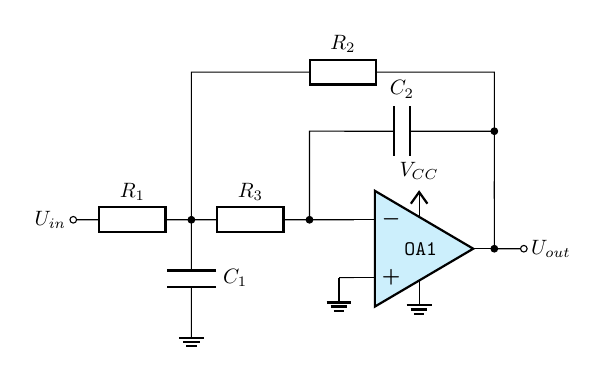
\begin{tikzpicture}[transform shape, use fpu reciprocal, scale=.75]
                \draw (0,0)
                    to[R, l=$R_1$, -*] ++(2,0)
                    coordinate(C1)
    
                    to[R, l=$R_3$, -*] ++(2,0)
                    coordinate(C2)
                    -- ++(.75,0)
                    node[op amp, noinv input down, fill=cyan!20, anchor=-](OA1){\texttt{OA1}}
    
                    (OA1.+)
                    -- ++(-.25,0)
                    node[ground]{}
    
                    (OA1.up)
                    node[vcc]{$V_{CC}$}
    
                    (OA1.down)
                    node[ground]{}
    
                    (C1)
                    to[C, l=$C_1$] ++(0,-2)
                    node[tlground]{}
    
                    (C2)
                    -- ++(0,1.5)
                    coordinate(R2start)
                    to[C, l=$C_2$, -*] (R2start-|OA1.out)
                    coordinate(R2)
                    to[short, -*] (OA1.out)
    
                    (C1)
                    -- ++(0,2.5)
                    coordinate(C3start)
                    to[R, l=$R_2$] (C3start-|OA1.out)
                    -- (R2)
    
                    (OA1.out) ++(.5,0)
                    node[right]{$U_{out}$}
                    to[short, o-] ++(-.5,0)
    
                    (0,0)
                    node[left]{$U_{in}$}
                    to[short, o-] ++(0,0)
                    ;
            \end{tikzpicture}
            \subcaption{Multiple-Feedback topology; its advantages are fewer passive components and lower sensitivity to changes in their values \emph{(Passive components do not have fully constant values; they depend mainly on the temperature of their environment)}, and it has the characteristic of inverting the signal}
            \label{fig:MFBSchematic}
        \end{minipage}
        \hspace{.04\linewidth}
        \caption{Diagram of two second-order active LPF circuits}
        \label{fig:SKMFBSchematic}
    \end{figure}


    \noindent To calculate the transfer function of these filters I applied the following technique:
    \begin{enumerate}[label=\emph{(\roman*)}]
        \item Use the functions obtained from the Laplace transform for the passive components.
        \item Use Ohm's laws and Kirchhoff's laws to write the circuit equations, i.e. the relations between the different currents present in the circuit
        \item Write a system of equations describing the relations between the different currents, defined in the form $I=\frac{U}{Z(s)}$
        \item Eliminate all currents except $\frac{U_{out}}{U_{in}}$
        \item Isolate $\frac{U_{out}}{U_{in}}$ on one side
    \end{enumerate}
    In this way I managed to describe the different types of the two circuit topologies; the interested reader can see them in the pages of Section \ref{sec:Calculations} on calculations.

    \clearpage
    \section{Sensor board}\label{sec:Sensorboard}
    \subsection{Characteristics}\label{sec:SensorboardCharacteristics}
    \begin{enumerate}[label=\emph{(\arabic*)}]
        \item Resistance to external noise, i.e. the ability to select the necessary part of the signal
        \item Resistance to mechanical shock
        \item Introduce as little internal or external noise into the circuit as possible to maintain high signal quality: aim for $12bit$ resolution\footcite[p9]{EMGBitdepth}
        \item Modularity
        \item Small size
    \end{enumerate}

    \subsection{Design}\label{sec:SensorboardDesign}
    To be able to make appropriate decisions one must first study the concrete situation.
    \subsubsection{Study of the input}\label{sec:SensorboardDesignInput}
    To study the input, one must also be informed about the source.
    The signals originating from the spinal cord, called APs\footnote{Action potentials \parenciteit{}{MerlettiMuceli}}, travel through the nerves according to the "All or None" law\footnote{Caused by the properties of nerve cells: precisely the voltage-gated sodium channels \parenciteit{}{SodiumChannel:Wiki} that create the chain reaction.}, a chain reaction that makes\footnote{Neurons in the inactive state have a negative potential of around $-70mV$ \parenciteit{}{AP:Wiki}} the neurons positive\footnote{If a neuron exceeds $-55mV$ the voltage-gated sodium channels open, letting sodium cations in, and consequently the neuron takes on a positive charge \parenciteit{}{AP:Wiki}} one after another, finally reaching the innervation of the muscle \footnote{Connection of the nerve with the muscle \parenciteit{"NMJ" and "innervation zone" p3}{MerlettiMuceli}}.
    Immediately afterwards the second chain reaction starts: that of the muscle.
    The muscle cells contract one after another, thereby activating the others, and the muscle signal \todo{Add the example of the decomposition of the signal into frequencies and the pure signal} is amplified many times, creating a signal like the one in Figure \ref{fig:ExampleEMGSignal} \ref{fig:ExampleEMGSignalTime}

    % TRANSLATOR NOTE: the first footnote below is unfinished in the original ("non ci sono separazioni "); translated as-is.
    It is worth noting that the intensity of the total signal\footnote{It should be understood that in this case there are no separations } has its largest amplitude towards low frequencies\footnote{This could also partly be the component introduced by flicker (pink) noise from the sensor circuits}.

    When the signal arrives via the nerve at the innervation of the muscle, the muscle cells start to contract\footnote{By contracting they in turn generate more signal, thereby amplifying the signal also for the other muscle cells}, they too creating a chain reaction through certain electrochemical processes.
    On the surface of human skin, at the moment the underlying muscles contract, electric fields are present.
    The peak voltage between the electrode receiving the signal and the electrode connected to an electrically neutral\footnote{Where no electric fields are present} skin surface is $10mV$ \footcite[p435]{Naik}\: \footcite[p1]{Xiaoou}.
    The frequency of the useful signal of a generic muscle is mainly between $20-500Hz$\footcite[p1]{EMGFreq}.
    The propagation of the signal is not instantaneous, but has a speed between $3-5m/s$\footcite[p2]{MerlettiMuceli}.
    The resistance of human skin, which must always be taken into account because of its influence on the peak current, can vary from $1k\Omega$ to $100k\Omega$\footcite["Under dry conditions, the resistance offered by the human body may be as high as 100,000Ohms.  Wet or broken skin may drop the body's resistance to 1,000 Ohms", p7]{ElectricalDeaths}.
    The variation of the above data depends on the quality of contact with the skin and on the correct placement of the electrodes.

    \begin{figure}[H]
        \centering
        \begin{minipage}[H]{\linewidth}
            \raggedright
            \begin{tikzpicture}
                \begin{axis}[
                    axis x line=bottom,
                    axis y line*=left,
                    ylabel style={rotate=-90},
                    xlabel={$t[ms]$},
                    ylabel={$U[V]\cdot k$},
                    legend entries={$($Channel $1)$, $($Channel $2)$, $($Channel $3)$, $($Channel $4)$, $($Channel $5)$, $($Channel $6)$, $($Channel $7)$, $($Channel $8)$},
                    legend pos=north east,
                    height=.4\textwidth,
                    width=.85\textwidth,
                    smooth,
                    clip=true,
                    xmin=2500,
                    xmax=17500,
                    axis_style_default_data,
                    colormap/twilight,
                    ymajorgrids=true,
                    xmajorgrids=false,
                    grid style=dashed,
                    cycle list={[colors of colormap={130,200,280,370,630,720,800,870},]},
                    every axis plot/.append style={mark=none, thick, draw opacity=.7},
                    ]
                    \begin{scope}[blend group=hard light]
                        \addplot table [x=time, y=channel1, col sep=comma]{datasets/cf_fft_hand_muscles/snip_s.csv};
                        \addplot table [x=time, y=channel2, col sep=comma]{datasets/cf_fft_hand_muscles/snip_s.csv};
                        \addplot table [x=time, y=channel3, col sep=comma]{datasets/cf_fft_hand_muscles/snip_s.csv};
                        \addplot table [x=time, y=channel4, col sep=comma]{datasets/cf_fft_hand_muscles/snip_s.csv};
                        \addplot table [x=time, y=channel5, col sep=comma]{datasets/cf_fft_hand_muscles/snip_s.csv};
                        \addplot table [x=time, y=channel6, col sep=comma]{datasets/cf_fft_hand_muscles/snip_s.csv};
                        \addplot table [x=time, y=channel7, col sep=comma]{datasets/cf_fft_hand_muscles/snip_s.csv};
                        \addplot table [x=time, y=channel8, col sep=comma]{datasets/cf_fft_hand_muscles/snip_s.csv};
                    \end{scope}
                \end{axis}
            \end{tikzpicture}
            \subcaption{A segment of signal consisting of 8 channels, from $($Channel $1)$ to $($Channel $8)$, as a function of time \emph{(the increase in amplitude corresponds to muscle tension)}}
            \label{fig:ExampleEMGSignalTime}
        \end{minipage}
        \vspace{3ex}
        \begin{minipage}[H]{\linewidth}
            \raggedright
            \begin{tikzpicture}
                \begin{axis}[
                    axis x line=bottom,
                    axis y line*=left,
                    ylabel style={rotate=-90},
                    xlabel={$f[Hz]$},
                    ylabel={$U[V]\cdot k$},
                    legend entries={$(a)$ Total, $(b)$ Noise},
                    legend pos=north east,
                    height=.305\textwidth,
                    width=.8\textwidth,
                    smooth,
                    clip=true,
                    xmode=log,
                    ymode=log,
                    domain=1:500,
                    samples=50,
                    xmin=1,
                    xmax=500,
                    ymin=2e-8,
                    ymax=3e-5,
                    axis_style_default_data,
                    colormap/twilight_shifted,
                    ymajorgrids=true,
                    xmajorgrids=true,
                    grid style=dashed,
                    cycle list={[colors of colormap={145,250},]},
                    every axis plot/.append style={mark=none, thick, draw opacity=.7},
                    ]
                    \begin{scope}[blend group=hard light]
                        \addplot table [x=freqs, y=spect, col sep=comma]{datasets/cf_fft_hand_muscles/sfft.csv};
                        \addplot table [x=freqs, y=spect, col sep=comma]{datasets/cf_fft_hand_muscles/noise_sfft.csv};
                    \end{scope}
                \end{axis}
            \end{tikzpicture}
            \subcaption{Frequency spectrum of the total average $(a)$ and of the noise average $(b)$}
            \label{fig:ExampleEMGSignalFFT}
        \end{minipage}
        \vspace{3ex}
        \begin{minipage}[H]{\linewidth}
            \raggedright
            \begin{tikzpicture}
                \begin{axis}[
                    axis x line=bottom,
                    axis y line*=left,
                    ylabel style={rotate=-90},
                    xlabel={$f[Hz]$},
                    ylabel={$U[V]\cdot k$},
                    legend entries={$(c)$ Extended palm (raw), $(d)$ Fist (raw)},
                    legend pos=north east,
                    height=.305\textwidth,
                    width=.8\textwidth,
                    smooth,
                    clip=true,
                    xmode=log,
                    ymode=log,
                    domain=1:500,
                    samples=50,
                    xmin=1,
                    xmax=500,
                    ymin=2e-8,
                    ymax=3e-5,
                    axis_style_default_data,
                    colormap/twilight_shifted,
                    ymajorgrids=true,
                    xmajorgrids=true,
                    grid style=dashed,
                    cycle list={[colors of colormap={280,720},]},
                    every axis plot/.append style={mark=none, thick, draw opacity=.7},
                    ]
                    \begin{scope}[blend group=hard light]
                        \addplot table [x=freqs, y=spect, col sep=comma]{datasets/cf_fft_hand_muscles/extended_sfft.csv};
                        \addplot table [x=freqs, y=spect, col sep=comma]{datasets/cf_fft_hand_muscles/fist_sfft.csv};
                    \end{scope}
                \end{axis}
            \end{tikzpicture}
            \subcaption{Frequency spectrum of the average, without noise subtraction, during the extended-palm gesture $(c)$ and during the fist gesture $(d)$}
            \label{fig:ExampleEMGSignalFFTGestures}
        \end{minipage}
        \vspace{3ex}
        \begin{minipage}[H]{\linewidth}
            \raggedright
            \begin{tikzpicture}
                \begin{axis}[
                    axis x line=bottom,
                    axis y line*=left,
                    ylabel style={rotate=-90},
                    xlabel={$f[Hz]$},
                    ylabel={$U[V]\cdot k$},
                    legend entries={$(e)$ Extended palm, $(f)$ Fist},
                    legend pos=north east,
                    height=.305\textwidth,
                    width=.8\textwidth,
                    smooth,
                    clip=true,
                    xmode=log,
                    ymode=log,
                    domain=1:500,
                    samples=50,
                    xmin=1,
                    xmax=500,
                    ymin=2e-8,
                    ymax=3e-5,
                    axis_style_default_data,
                    colormap/twilight_shifted,
                    ymajorgrids=true,
                    xmajorgrids=true,
                    grid style=dashed,
                    cycle list={[colors of colormap={750,855},]},
                    every axis plot/.append style={mark=none, thick, draw opacity=.7},
                    ]
                    \begin{scope}[blend group=hard light]
                        \addplot table [x=freqs, y=spect, col sep=comma]{datasets/cf_fft_hand_muscles/extended_filt_sfft.csv};
                        \addplot table [x=freqs, y=spect, col sep=comma]{datasets/cf_fft_hand_muscles/fist_filt_sfft.csv};
                    \end{scope}
                \end{axis}
            \end{tikzpicture}
            \subcaption{Frequency spectrum of the average, after noise subtraction, during the extended-palm gesture $(e)$ and during the fist gesture $(f)$}
            \label{fig:ExampleEMGSignalFFTGesturesPure}
        \end{minipage}
        \caption{Example of the muscle AP signal measured in $U[V]\cdot k$ \emph{(}$k$\emph{ denotes the unknown amplification of the read and digitized voltages shown in the plots)}, as a function of time in \ref{fig:ExampleEMGSignalTime} and decomposed into frequencies \emph{(i.e. into the frequency spectrum)} with the Fourier transform in plots \ref{fig:ExampleEMGSignalFFT}, \ref{fig:ExampleEMGSignalFFTGestures}, \ref{fig:ExampleEMGSignalFFTGesturesPure} \emph{\parenciteit{}{EMGData}}}
        \label{fig:ExampleEMGSignal}
    \end{figure}

    \subsubsection{Study of the output}\label{sec:SensorboardDesignOutput}
    The output depends entirely on the ADC chosen.
    It suffices that the output of the analog circuit\footnote{Output of the filters} fits within the predefined limits of the integrated circuit.
    As good practice, I believe the maximum signal amplitude should be multiplied by 4 to obtain the ADC input limits, to prevent signal clipping.
    The output obviously cannot be negative, so as not to risk exceeding the ADC specifications.
    The solution would be a half-wave\footnote{The signal will be cut off if it falls below a certain voltage threshold} or full-wave\footnote{The signal is inverted if it falls below a certain voltage threshold} precision rectifier.
    The maximum voltage must not exceed the limits either, which is why I would use precision linear voltage sources\footnote{The voltage needs to be stable and the converter must not create EMI problems, which is why "switch-mode" DC-DC converters cannot be used directly, as said in Section \ref{sec:MotherboardDesignSupply}} not exceeding the maximum allowed voltage.

    \subsubsection{Circuit} \label{sec:SensorBoardSchematic}
    The sensor board circuit must first of all eliminate the external interference reaching the electrodes.
    We can use the characteristic latency of signal propagation through the muscle: the external interference reaching the two\footnote{Minimum number of electrodes we need to attenuate a large part of the interference in the signal} electrodes tends to be instantaneous, like RF, whereas the difference in distance between the electrodes has an impact on the muscle signal they read.
    For this reason it is enough for us to subtract the two signals.
    In circuit design practice there is an active component designed for the subtraction\footnote{It nevertheless has the characteristic of being analog} of two signals, called an INA, or instrumentation amplifier.
    \begin{figure}[H]
        \centering
        \hspace{.02\linewidth}
        \begin{minipage}[H]{.24\linewidth}
            \centering
            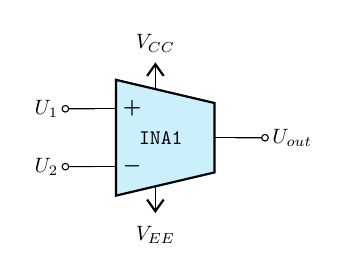
\begin{tikzpicture}[transform shape, use fpu reciprocal, scale=.75]
                \draw (0,0)
                    node[inst amp, noinv input up, fill=cyan!20](INA1){\texttt{INA1}}
                    \opampPMCenter{INA1}

                    (INA1.+) ++(-.5,0)
                    node[left]{$U_1$}
                    to[short, o-] ++(.5,0)

                    (INA1.-) ++(-.5,0)
                    node[left]{$U_2$}
                    to[short, o-] ++(.5,0)

                    (INA1.up)
                    node[vcc]{$V_{CC}$}

                    (INA1.down)
                    node[vee]{$V_{EE}$}

                    (INA1.out) ++(.5,0)
                    node[right]{$U_{out}$}
                    to[short, o-] ++(-.5,0)
                    ;
            \end{tikzpicture}
            \subcaption{The INA symbol; it is powered by two voltage sources, $V_{CC}$ the positive and $V_{EE}$ the negative one, with $U_1$ an input signal at the $+$ input, another input signal $U_2$ at the inverting input $-$ \emph{(It multiplies the signal by $-1$)} and an output $U_{out}$}
            \label{fig:INASymbol}
        \end{minipage}
        \hspace{.04\linewidth}
        \begin{minipage}[H]{.64\linewidth}
            \centering
            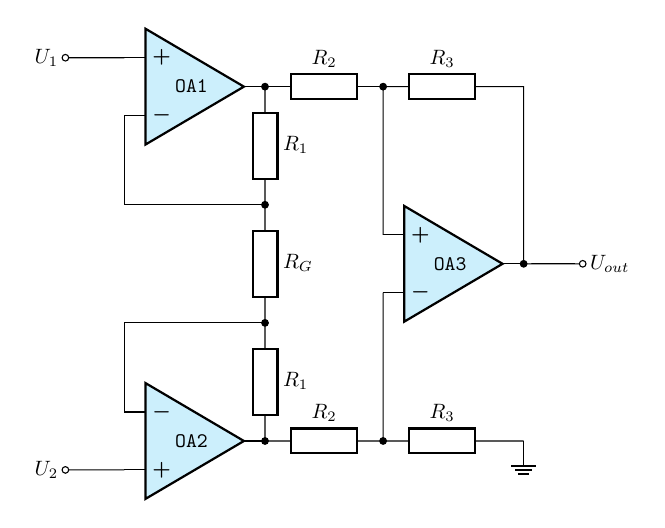
\begin{tikzpicture}[transform shape, use fpu reciprocal, scale=.75]
                \draw (0,0)
                    node[op amp, noinv input up, fill=cyan!20](OA1){\texttt{OA1}}
                    \opampPMCenter{OA1};
                \draw (OA1.+) ++(-1,0)
                    node[left]{$U_1$}
                    to[short, o-] ++(1,0);
                \draw (OA1.out)
                    to[short, -*] ++(0,0)
                    to[R, l=$R_1$, -*] ++(0,-2)
                    coordinate(OA1-R1Rg)
                    to[R, l=$R_{G}$, -*] ++(0,-2)
                    coordinate(OA2-R1Rg)
                    to[R, l=$R_1$, -*] ++(0,-2)
                    node[op amp, fill=cyan!20, anchor=out](OA2){\texttt{OA2}};
                \draw (OA2.+) ++(-1,0)
                    node[left]{$U_2$}
                    to[short, o-] ++(1,0);
                \draw (OA1-R1Rg)
                    -- (OA1.- |- OA1-R1Rg)
                    -- (OA1.-);
                \draw (OA2-R1Rg)
                    -- (OA2.- |- OA2-R1Rg)
                    -- (OA2.-);
                \draw (OA1.out)
                    to[R, l=$R_2$, -*] ++(2,0)
                    coordinate(R2R3-up);
                \draw (OA2.out)
                    to[R, l=$R_2$, -*] ++(2,0)
                    coordinate(R2R3-down);
                \draw ($(R2R3-up)!.5!(R2R3-down)$) ++(opampPMCenter)
                    node[op amp, noinv input up, fill=cyan!20, anchor=center](OA3){\texttt{OA3}};
                \draw (OA3.+)
                    -- (R2R3-up);
                \draw (OA3.-)
                    -- (R2R3-down);
                \draw (R2R3-up)
                    to[R, l=$R_3$] ++(2,0)
                    -- (OA3.out |- R2R3-up)
                    to[short, -*](OA3.out)
                    coordinate(OA3-Vout);
                \draw (OA3.out) ++(1,0)
                    node[right]{$U_{out}$}
                    to[short, o-] ++(-1,0);
                \draw (R2R3-down)
                    to[R, l=$R_3$] ++(2,0)
                    -- (OA3.out |- R2R3-down)
                    node[ground]{};
            \end{tikzpicture}
            \subcaption{The internal composition of the INA: the gain is set by the resistor $R_G$, which is normally not included in the integrated circuit so that the circuit designer can choose the coefficient}
            \label{fig:INAInternalSchematic}
        \end{minipage}
        \hspace{.04\linewidth}
        \caption{Diagrams of a generic INA}
        \label{fig:INASchematic}
    \end{figure}

    The second type of interference is the one belonging to the frequency spectrum, which we identified from information in scientific articles and from the dataset in the plot in Figure \ref{fig:ExampleEMGSignal}.
    This is exactly where I decided to use two frequency filters of MFB topology, for the following reasons:
    \begin{itemize}
        \item I do not need to vary the shape of the transfer function
        \item I do not need to vary the signal gain\footnote{The variation can take place entirely at the INA stage of the chain}
        \item It would be useful to have fewer deviations from the designed transfer function due to variations in passive component values
        \item It would be useful for the circuit to take up less space\footnote{Thinking from the point of view of mass production, using as few components as possible is desirable}
        \item I do not mind whether the signal is inverted or not\footnote{It is enough that all digitized signals are inverted in the same way}
    \end{itemize}
    
    \noindent In the following pages I include the final circuit documents\footnote{I used the KiCad software to draw them} of the sensor board \emph{(Figures \ref{fig:CircuitDiagramSensorBoard} \ref{fig:CircuitDiagramSensorBoardCMRBPF} \ref{fig:CircuitDiagramSensorBoardRECT})}.
    \begin{figure}[H]
        \centering
        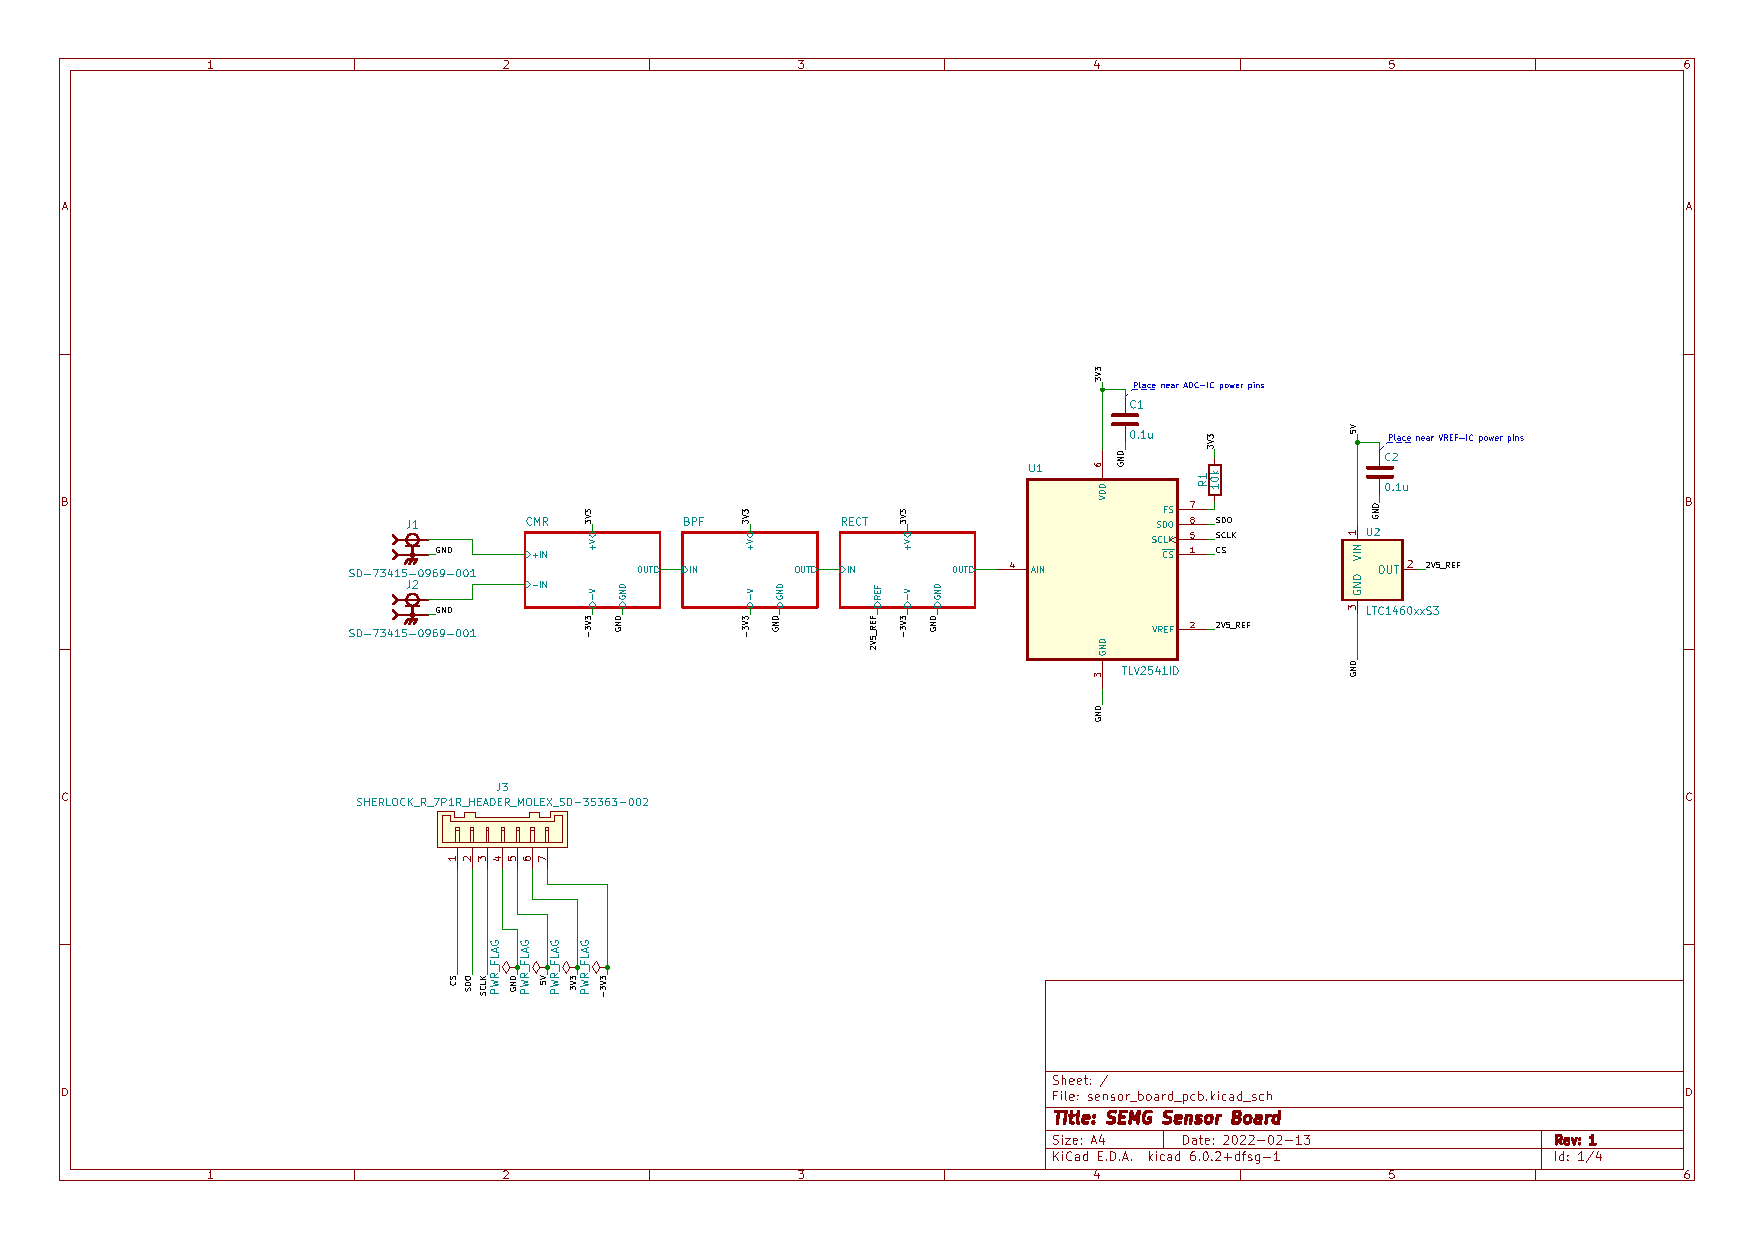
\includegraphics[height=\textwidth, angle=90]{media/sensor_board_pcb.pdf}
        \caption{Top-level hierarchical circuit of the sensor board, containing three stages \emph{(CMR, BPF, RECT)} shown in the following Figures \ref{fig:CircuitDiagramSensorBoardCMR}, \ref{fig:CircuitDiagramSensorBoardBPF}, \ref{fig:CircuitDiagramSensorBoardRECT} and an ADC}
        \label{fig:CircuitDiagramSensorBoard}
    \end{figure}
    \begin{figure}[H]
        \begin{minipage}[H]{\linewidth}
            \centering
            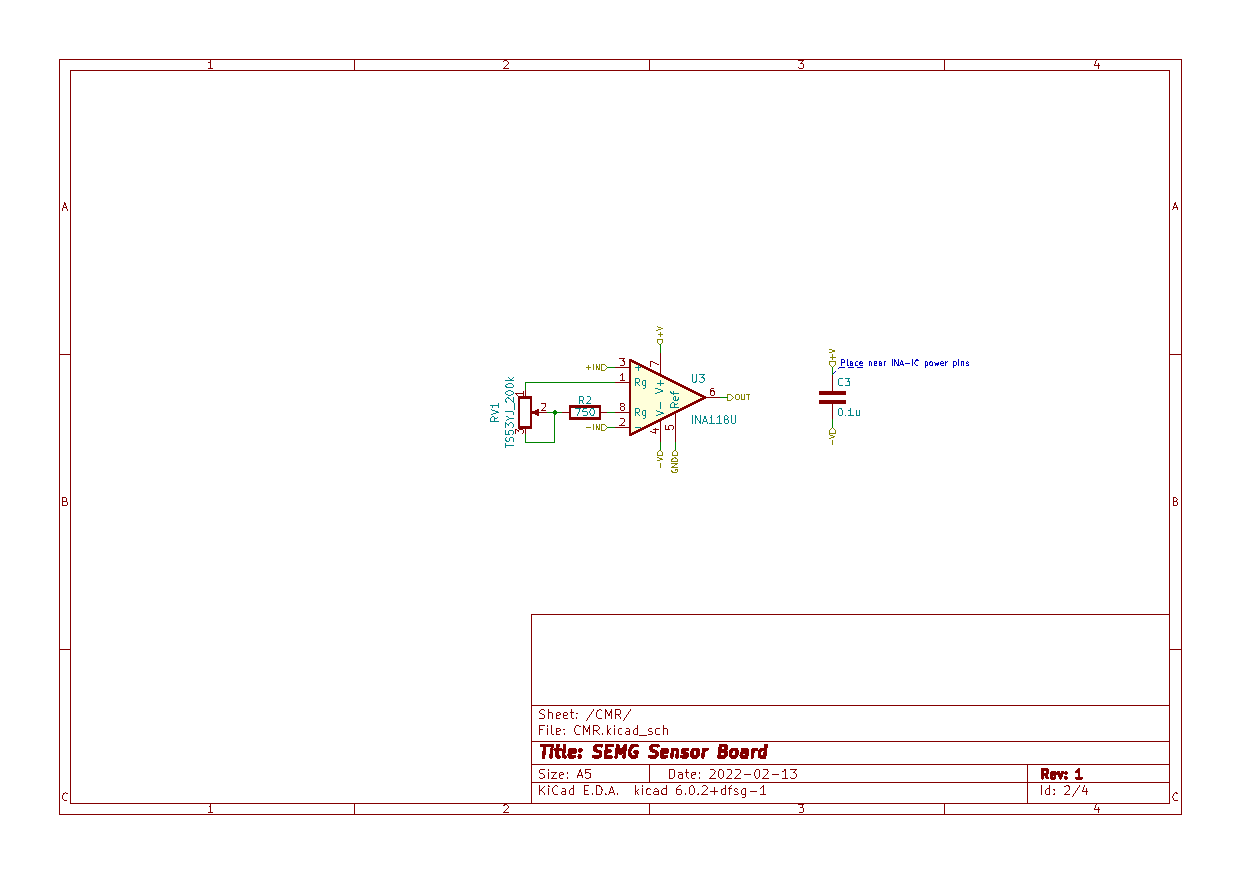
\includegraphics[width=\textwidth]{media/sensor_board_pcb-CMR.pdf}
            \subcaption{Circuit consisting of an INA to filter the signal, keeping the differing parts and attenuating the identical parts}
            \label{fig:CircuitDiagramSensorBoardCMR}
        \end{minipage}
        \begin{minipage}[H]{\linewidth}
            \centering
            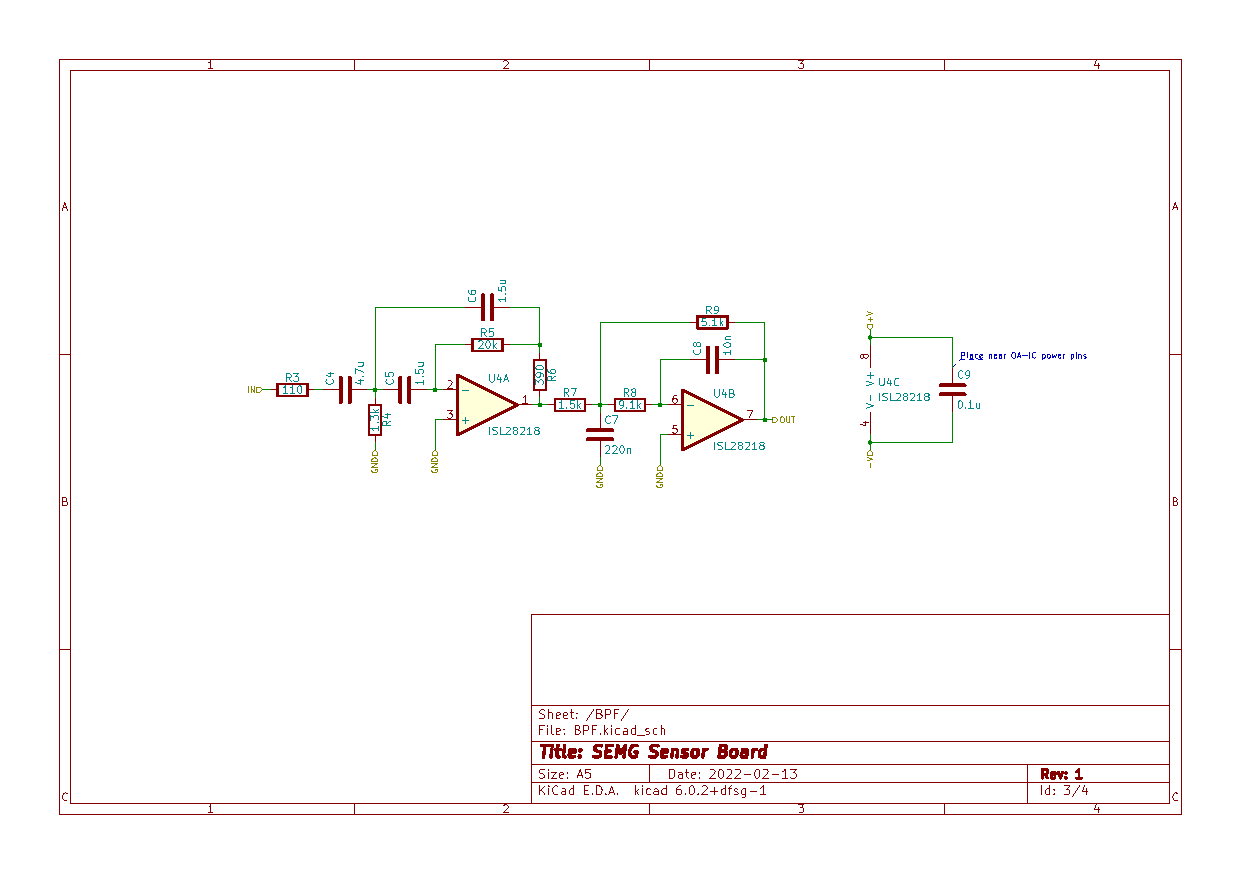
\includegraphics[width=\textwidth]{media/sensor_board_pcb-BPF.pdf}
            \subcaption{Circuit consisting of an HPF and an LPF of MFB topology to filter the $20-500Hz$ signal band  \emph{(The circuit inverts the signal twice)}}
            \label{fig:CircuitDiagramSensorBoardBPF}
        \end{minipage}
        \caption{}
        \label{fig:CircuitDiagramSensorBoardCMRBPF}
    \end{figure}
    \begin{figure}[H]
        \centering
        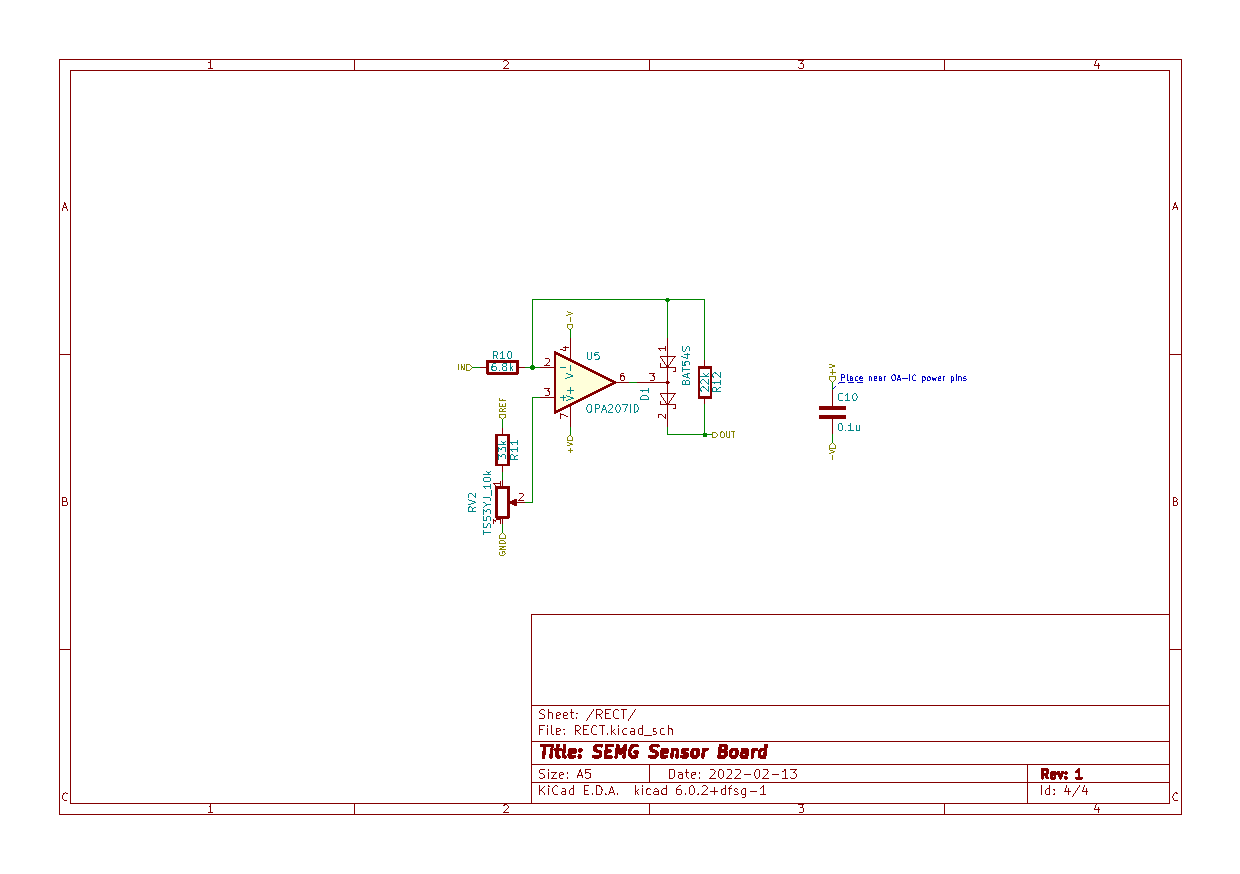
\includegraphics[width=\textwidth]{media/sensor_board_pcb-RECT.pdf}
        \caption{Circuit for rectifying the signal \emph{(In this topology the signal is inverted and its negative part is cut off)}}
        \label{fig:CircuitDiagramSensorBoardRECT}
    \end{figure}

    \noindent The circuits I included are:
    \begin{itemize}
        \item SEMG Sensor Board --- the sensor board
        \item SEMG Sensor Board - CMR --- the INA part, which I named this way after Common Mode Rejection
        \item SEMG Sensor Board - BPF --- the frequency filtering part, which serves to filter the $20-500Hz$ frequency band
        \item SEMG Sensor Board - RECT --- the signal rectification part\footnote{The ADC cannot receive a negative voltage below $0.3V$ \parenciteit{p8}{TLV2541:Datasheet}}
    \end{itemize}
    The circuit runs from two sources, one negative and one positive; they are needed by the INA to set the reference voltage at the level of the body, and to handle the signal when we use an HPF\footnote{All low-frequency and DC components are filtered out, centering the signal around $0V$}.
    % TRANSLATOR NOTE: "LTO regulator" kept as in the original; almost certainly means LDO.
    I added the circuit named "SEMG Sensor Board - RECT" so as not to exceed the ADC voltage limits, even though the signal can be centered around a value between $2.5-0V$\footnote{The $2.5V$ are provided by the fixed $2.5V$ LTO regulator $U2$} set by the potentiometer $RV2$.
    The signal amplitude is adjusted by the potentiometer $RV1$\footnote{At the last moment I discovered that the gain values I had calculated were inaccurate, and I changed the value of resistor $R2$ from $10k\Omega$ to $750\Omega$, thereby increasing the maximum gain of the circuit}.
    The other modifications that can be noticed with respect to the conceptual circuit proposed in much of Section \ref{sec:FilterTheory} are the resistors $R3$ and $R6$\footnote{There are two resistors so as not to modify the transfer function}\:\footnote{The values of these resistors were obtained from simulations in KiCad by tuning (trial and error)}, which serve to limit the maximum current that can flow from the output of the amplifier $U4A$ or the INA $U3$ at very high frequencies, which reduce the impedance of the capacitors $C6$ and $C4$ and could thereby cause $U3$ or $U4A$ to malfunction.
    Moreover, one notices the capacitors $C1$, $C2$, $C3$, $C9$, and $C10$, which have their own name, bypass capacitors; their function is to suppress high-frequency noise on the power supply lines, which can come from the digital part of the circuit\footnote{Not only from the ADC, but also from the supply side, which is connected through connector $J3$}.
    The ADC has three pins that serve to transmit information with the SPI protocol, which are connected to connector $J3$.
    The other two connectors, $J1$ and $J2$, serve to connect the electrode cables\footnote{They are connected to GND because the electrode cable is shielded to reduce interference and because the electrodes have two contacts: one for reference and one for the signal itself}
    $R1$ is a formality dictated by the ADC datasheet\footcite[p5,p21]{TLV2541:Datasheet} to tell it which mode it must operate in.

    \subsubsection{Component selection}
    Having the filter formulas and the data from the component datasheets, I chose\footnote{Component selection was always carried out with the iterative "modus operandi" with the help of the component database of the chosen distributor \parencite[]{Mouser:Web}} the passive components by trial and error to balance various factors such as the noise\footnote{In the calculations in Section \ref{sec:Calculations}, I used only components with data on their white noise (equal across the whole spectrum) and pink or flicker noise (more pronounced at low frequencies)} generated by the circuit.

    Then I started running circuit simulations to obtain passive component values in standardized E series, with as many of them equal as possible to reduce the BOM\footnote{Bill of Materials, a term denoting the list of components to purchase in order to assemble the circuit}, but without compromising on the predefined parameters\footnote{Gain, filter cutoff frequencies and component noise (the magnitude of the noise is defined in the calculations in Section \ref{sec:Calculations})}.

    \begin{figure}[H]
        \centering
        \begin{minipage}[H]{\linewidth}
            \centering
            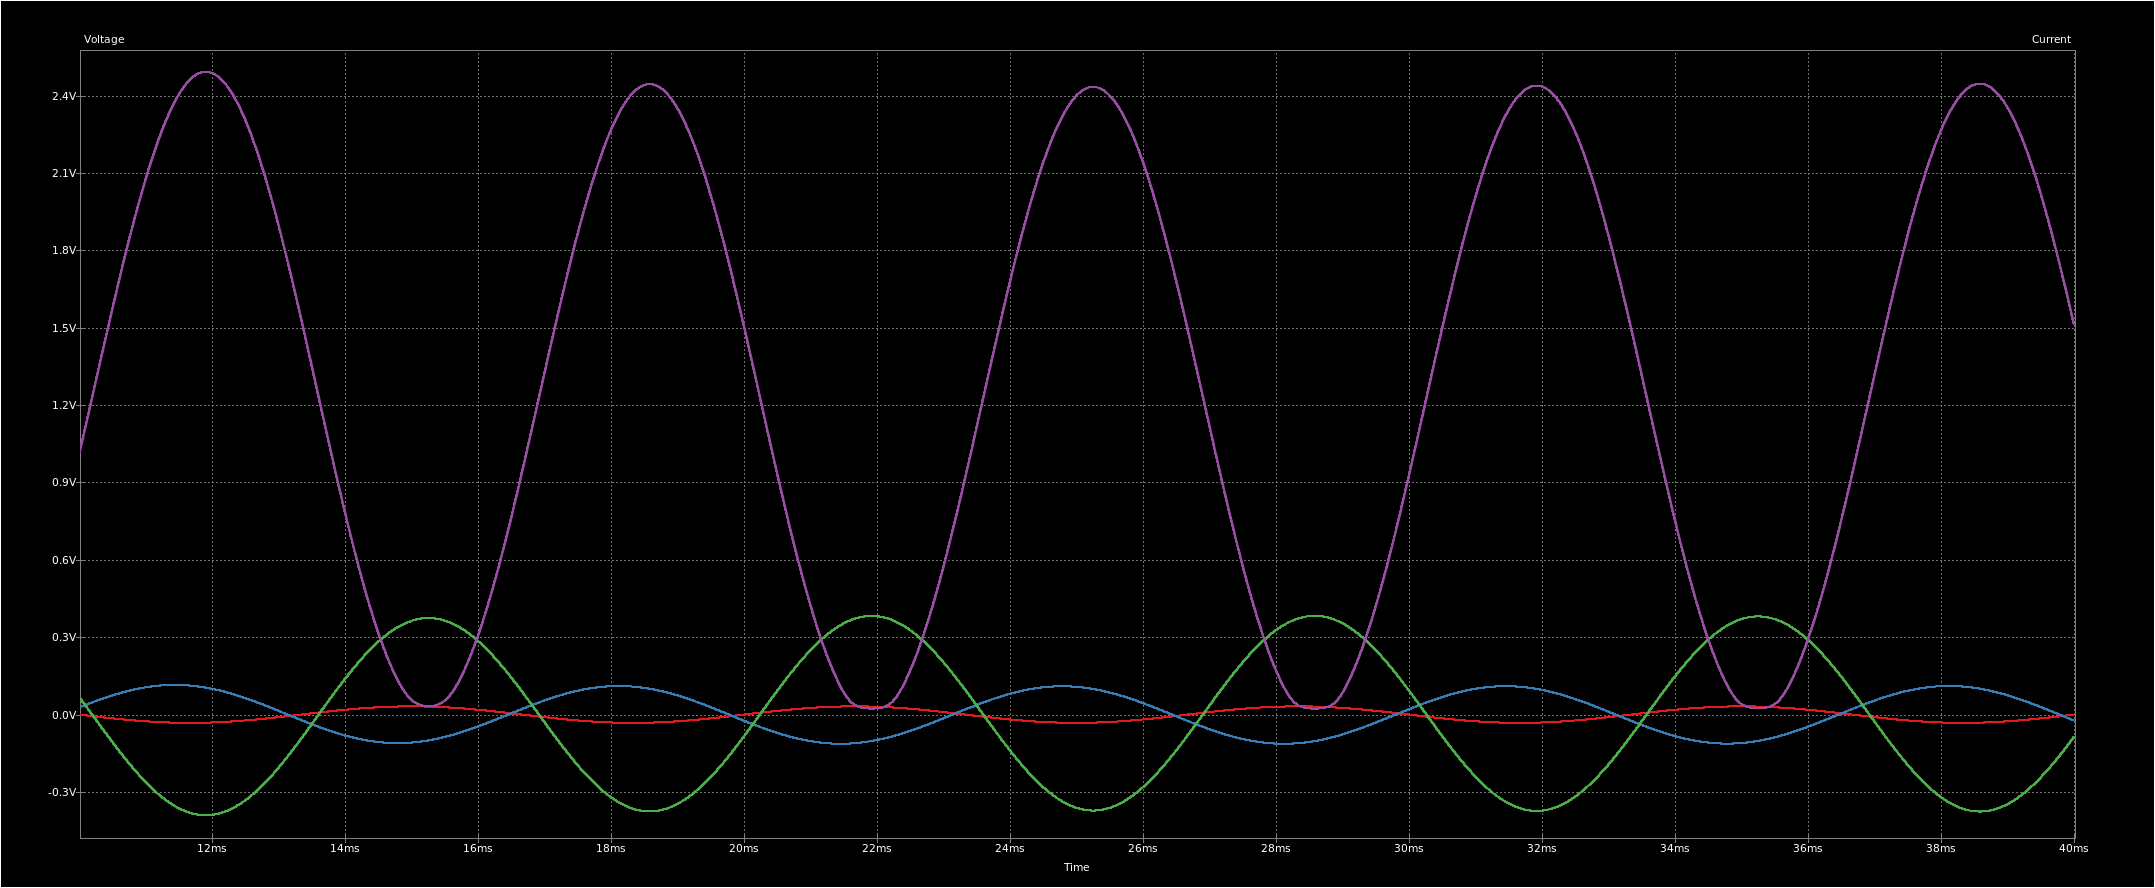
\includegraphics[width=\linewidth]{media/simtimeresp.png}
            \subcaption{Simulated time response of the circuit, with the red signal at the output of the hypothetical INA stage \emph{($SIG\_IN$)}, the blue signal at the output of the HPF \emph{(Output of $U1$)}, the green signal at the output of the LPF \emph{(Output of $U2$)} and the purple signal at the output of the rectifier \emph{($SIG\_OUT$)} \emph{(In this case the input signal to the frequency filter stage is $32mV$ at a frequency of $150Hz$, and it was centered around $1.25V$ at the last stage)}}
            \label{fig:timeresp}
        \end{minipage}
        \\
        \begin{minipage}[H]{\linewidth}
            \centering
            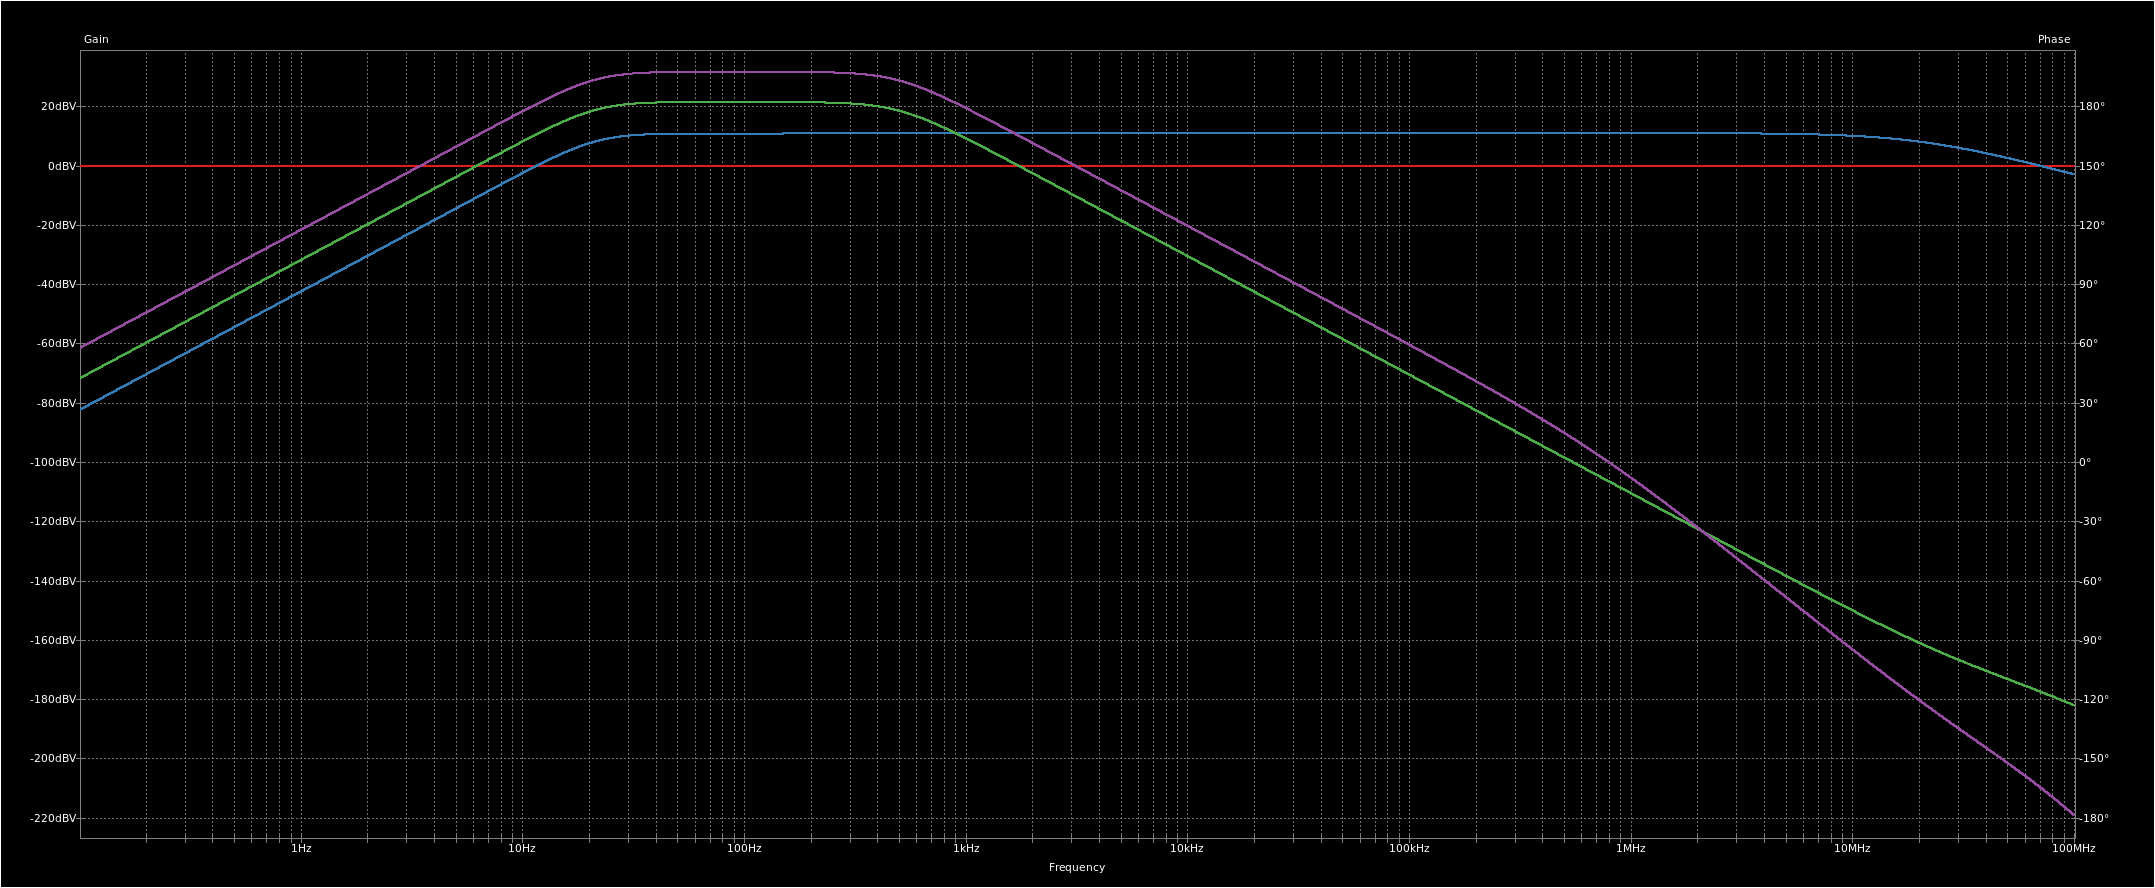
\includegraphics[width=\linewidth]{media/simfreqresp.png}
            \subcaption{Frequency response of the circuit, with the red signal at the output of the hypothetical INA \emph{($SIG\_IN$)}, the blue signal at the output of the HPF \emph{(Output of $U1$)}, the green signal at the output of the LPF \emph{(Output of $U2$)} and the purple signal at the output of the rectifier \emph{($SIG\_OUT$)}}
            \label{fig:freqresp}
        \end{minipage}
        \caption{Plots describing the behavior of the filter in the simulation}
        \label{fig:freqtimeresp}
    \end{figure}

    \begin{figure}[H]
        \centering
        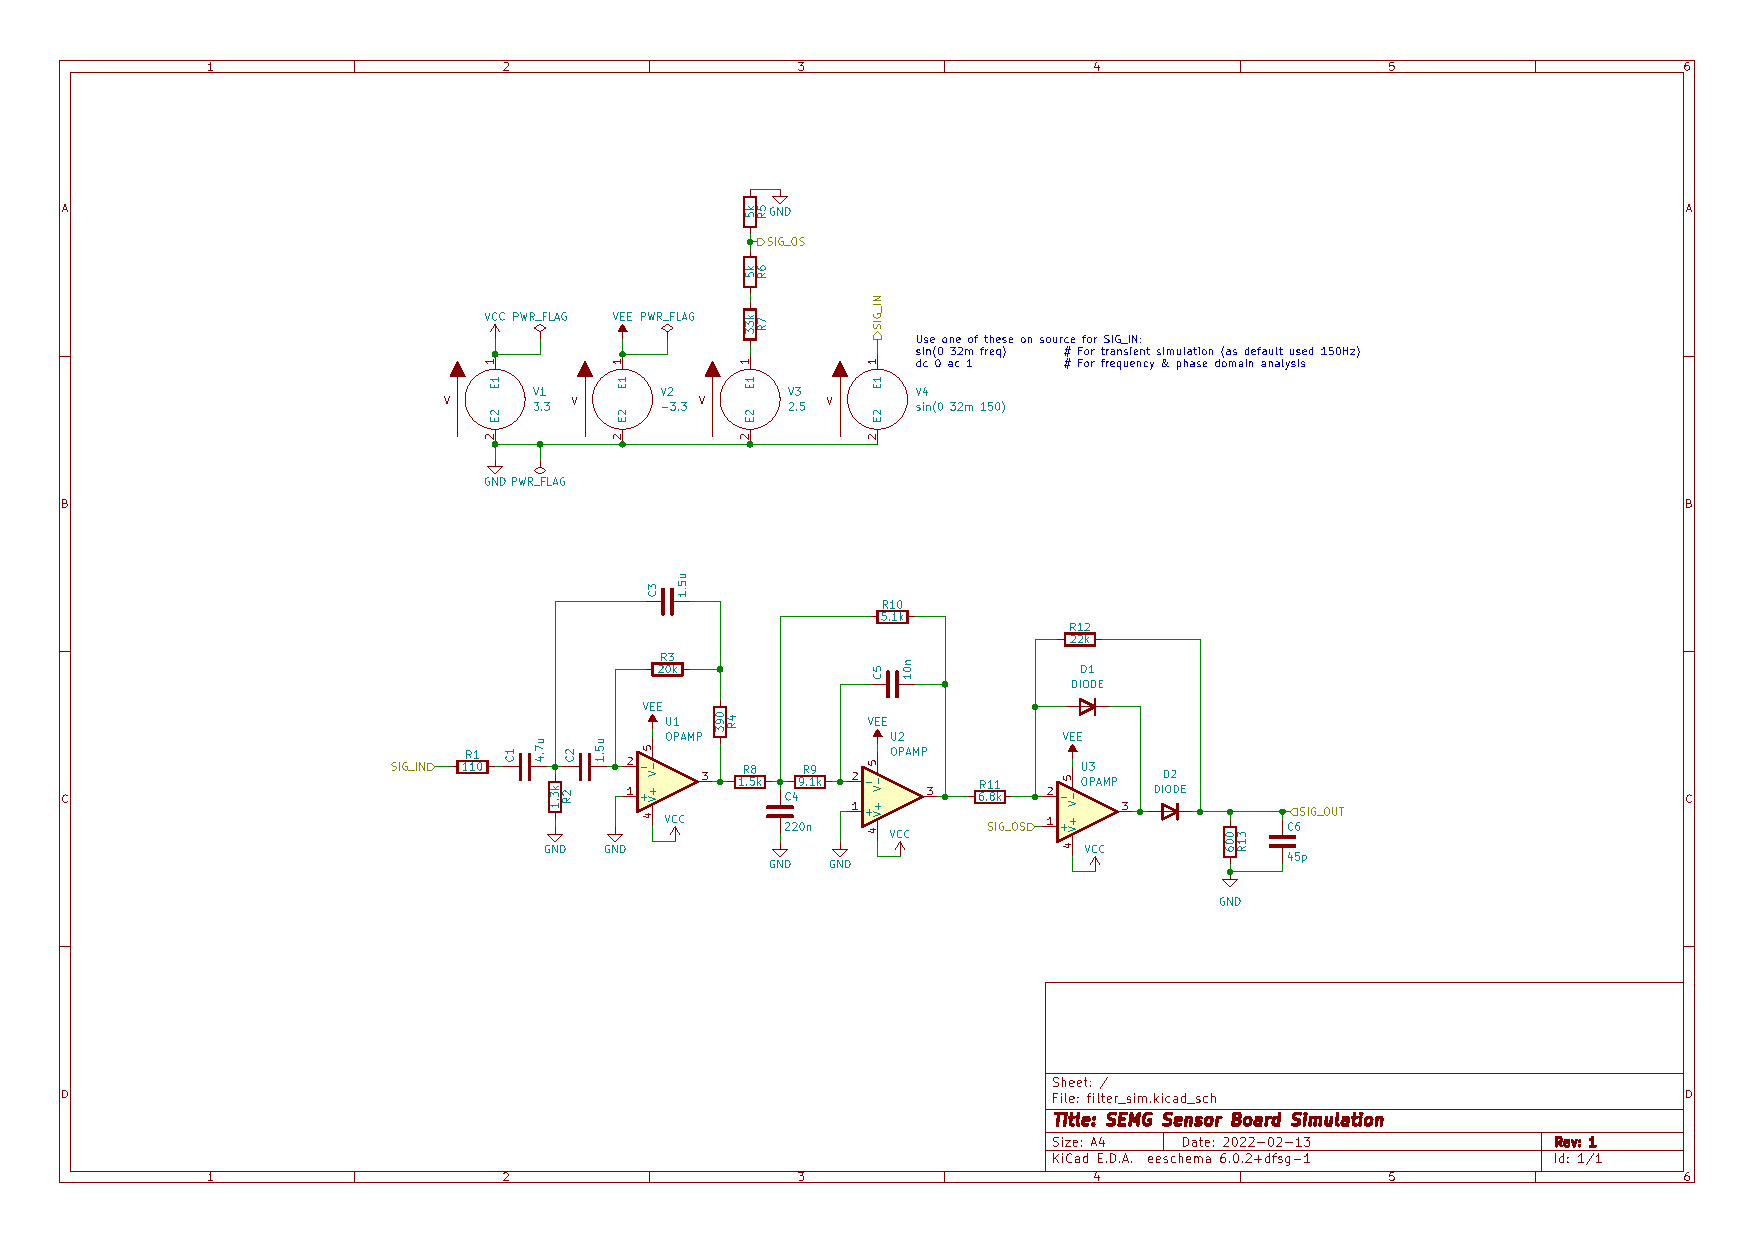
\includegraphics[height=\textwidth, angle=90]{media/filter_sim.pdf}
        \caption{The circuit in which the simulations were run}
    \end{figure}

    \noindent First, I chose an ADC suited to the $3.3V$ logic voltage and with $12bit$ resolution\footnote{With an SNR (Signal to Noise Ratio, the ratio of signal power to noise power) of approximately $72dB$, because that is the resolution itself converted into $[dB]$, as calculated in Section \ref{sec:Calculations}}.
    \todo{Put more detailed references to calculations (to single files)}

    % TRANSLATOR NOTE: the GBPW footnote is unfinished in the original ("Gain Bandwidth Power, oppure "); translated as-is ("..., or "). The standard term is Gain-Bandwidth Product (GBW/GBP).
    To choose the active components\footnote{Meaning the integrated circuits labeled $UX$ in the circuit in Figures \ref{fig:CircuitDiagramSensorBoard} \ref{fig:CircuitDiagramSensorBoardCMRBPF} \ref{fig:CircuitDiagramSensorBoardRECT}} of the analog part, I tried to calculate the minimum and maximum values of various characteristics for each component, such as GBPW\footnote{Gain Bandwidth Power, or }, slew rate\footnote{The reaction speed of the amplifier, i.e. how much its voltage can change in a given time interval (measured in $[V/\mu s]$)}, maximum output currents and others\footnote{They can be seen in Section \ref{sec:Calculations}}, for the OAs and the INA, to match them to the chosen ADC

    \subsubsection{Layout}
    For the layout\footnote{The arrangement of the components and of the traces that will act as conductors} of the board I chose similar component footprints, i.e. all integrated circuits are in SOIC-8 format\footcite[]{SOIC:Wiki}, the diodes and the voltage reference are in SOT-223 format\footcite[]{SOT:Wiki} and the passive components are size 1608\footnote{Metric}\:\footcite[]{SMT:Wiki}, so that they can be comfortably soldered with a soldering iron without compromising the small size of the circuit.

    Naturally, for the board I chose the variant with the fewest layers possible, to reduce the complexity of the circuit and to be able to make it at home with the clothes-iron method\footnote{Described in Section \ref{sec:BuildingHardware}} and chemical etching\footnote{Described in Section \ref{sec:BuildingHardware}}.
    Moreover, I dedicated the bottom layer to GND to improve the decoupling\footnote{All components also introduce noise into the supply when they draw different amounts of current at different instants} of the components, as good practice.

    The trace width was chosen arbitrarily\footnote{The contribution of the skin effect \parenciteit{}{SkinEffect:Wiki} can be ignored at low frequencies such as those we work with}

    \begin{figure}[H]
        \centering
        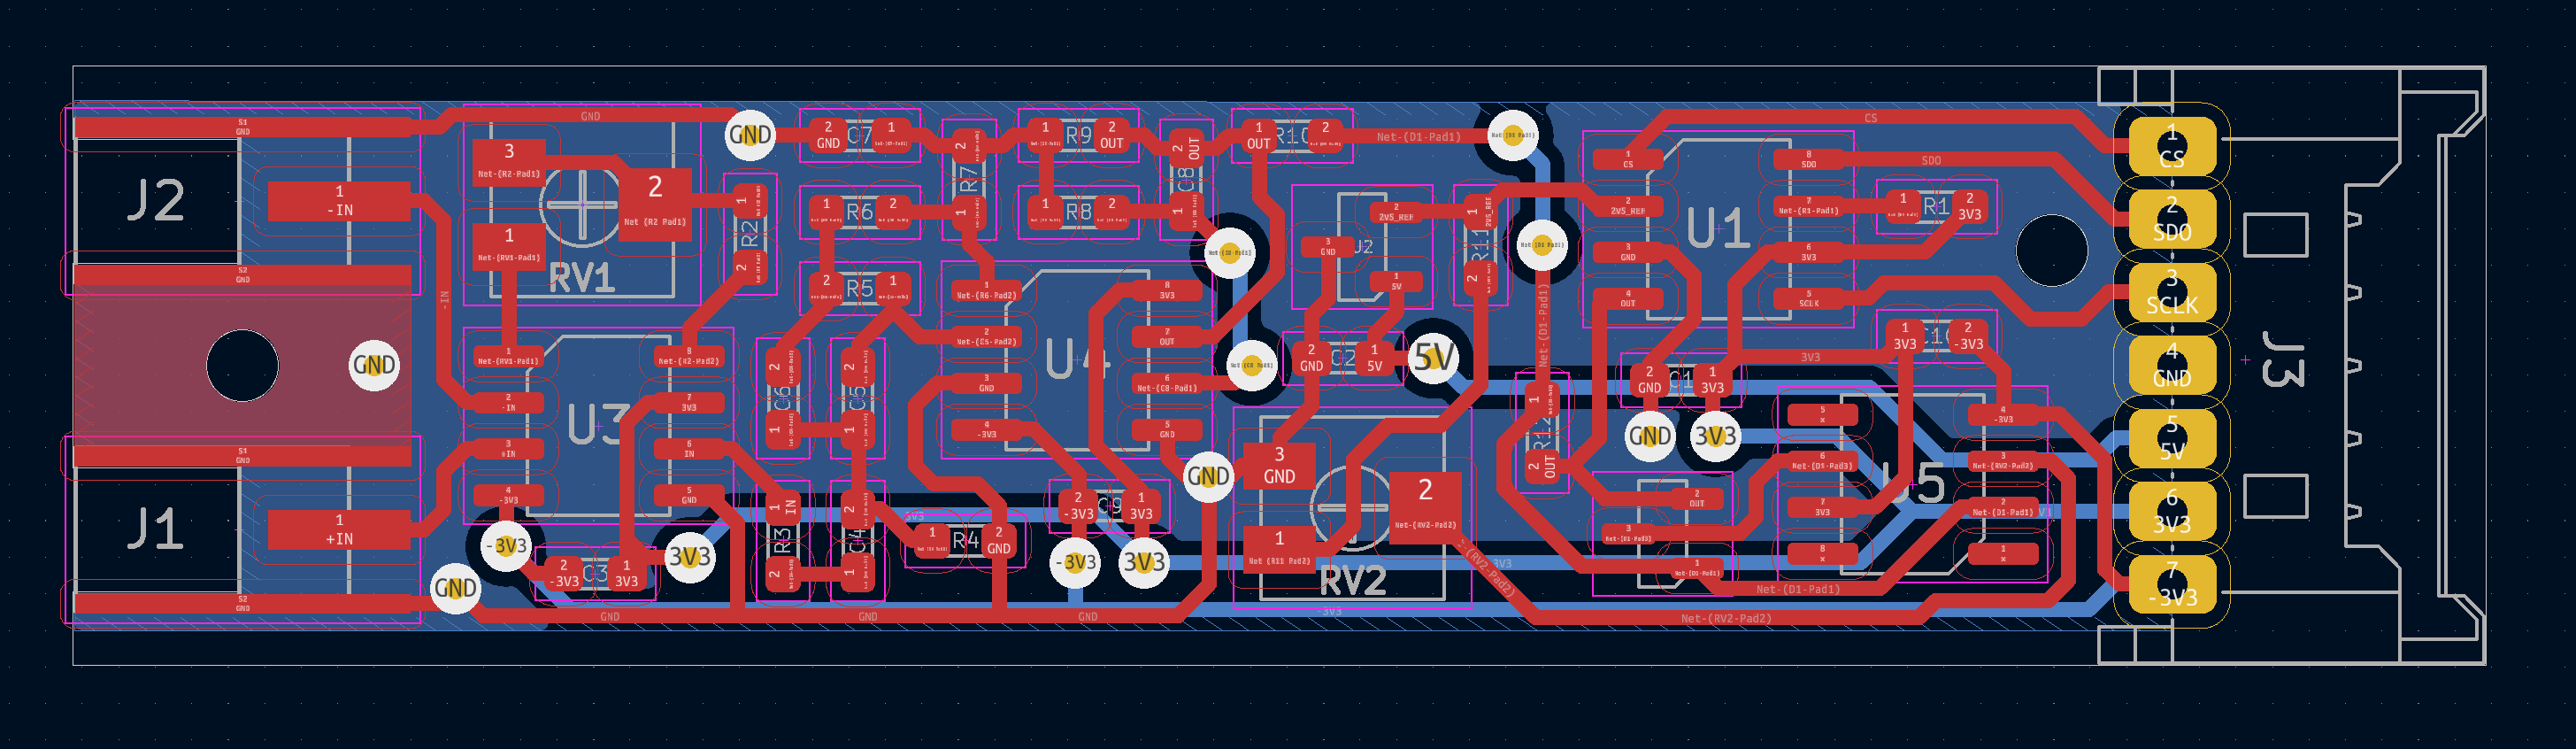
\includegraphics[width=\linewidth]{media/Layout.png}
        \caption{Layout of the sensor board, with the bottom copper layer of the board in blue and the top copper layer in red; the vias are the small yellow and white circles}
        \label{fig:Layout}
    \end{figure}
    \clearpage

    \section{Construction}\label{sec:Building}
    \subsection{Hardware}\label{sec:BuildingHardware}
    First I printed some variations of the circuit on sheets of office paper\footnote{Figure \ref{fig:BuildingHardwarePaperSheet}}.
    \begin{figure}[H]
        \centering
        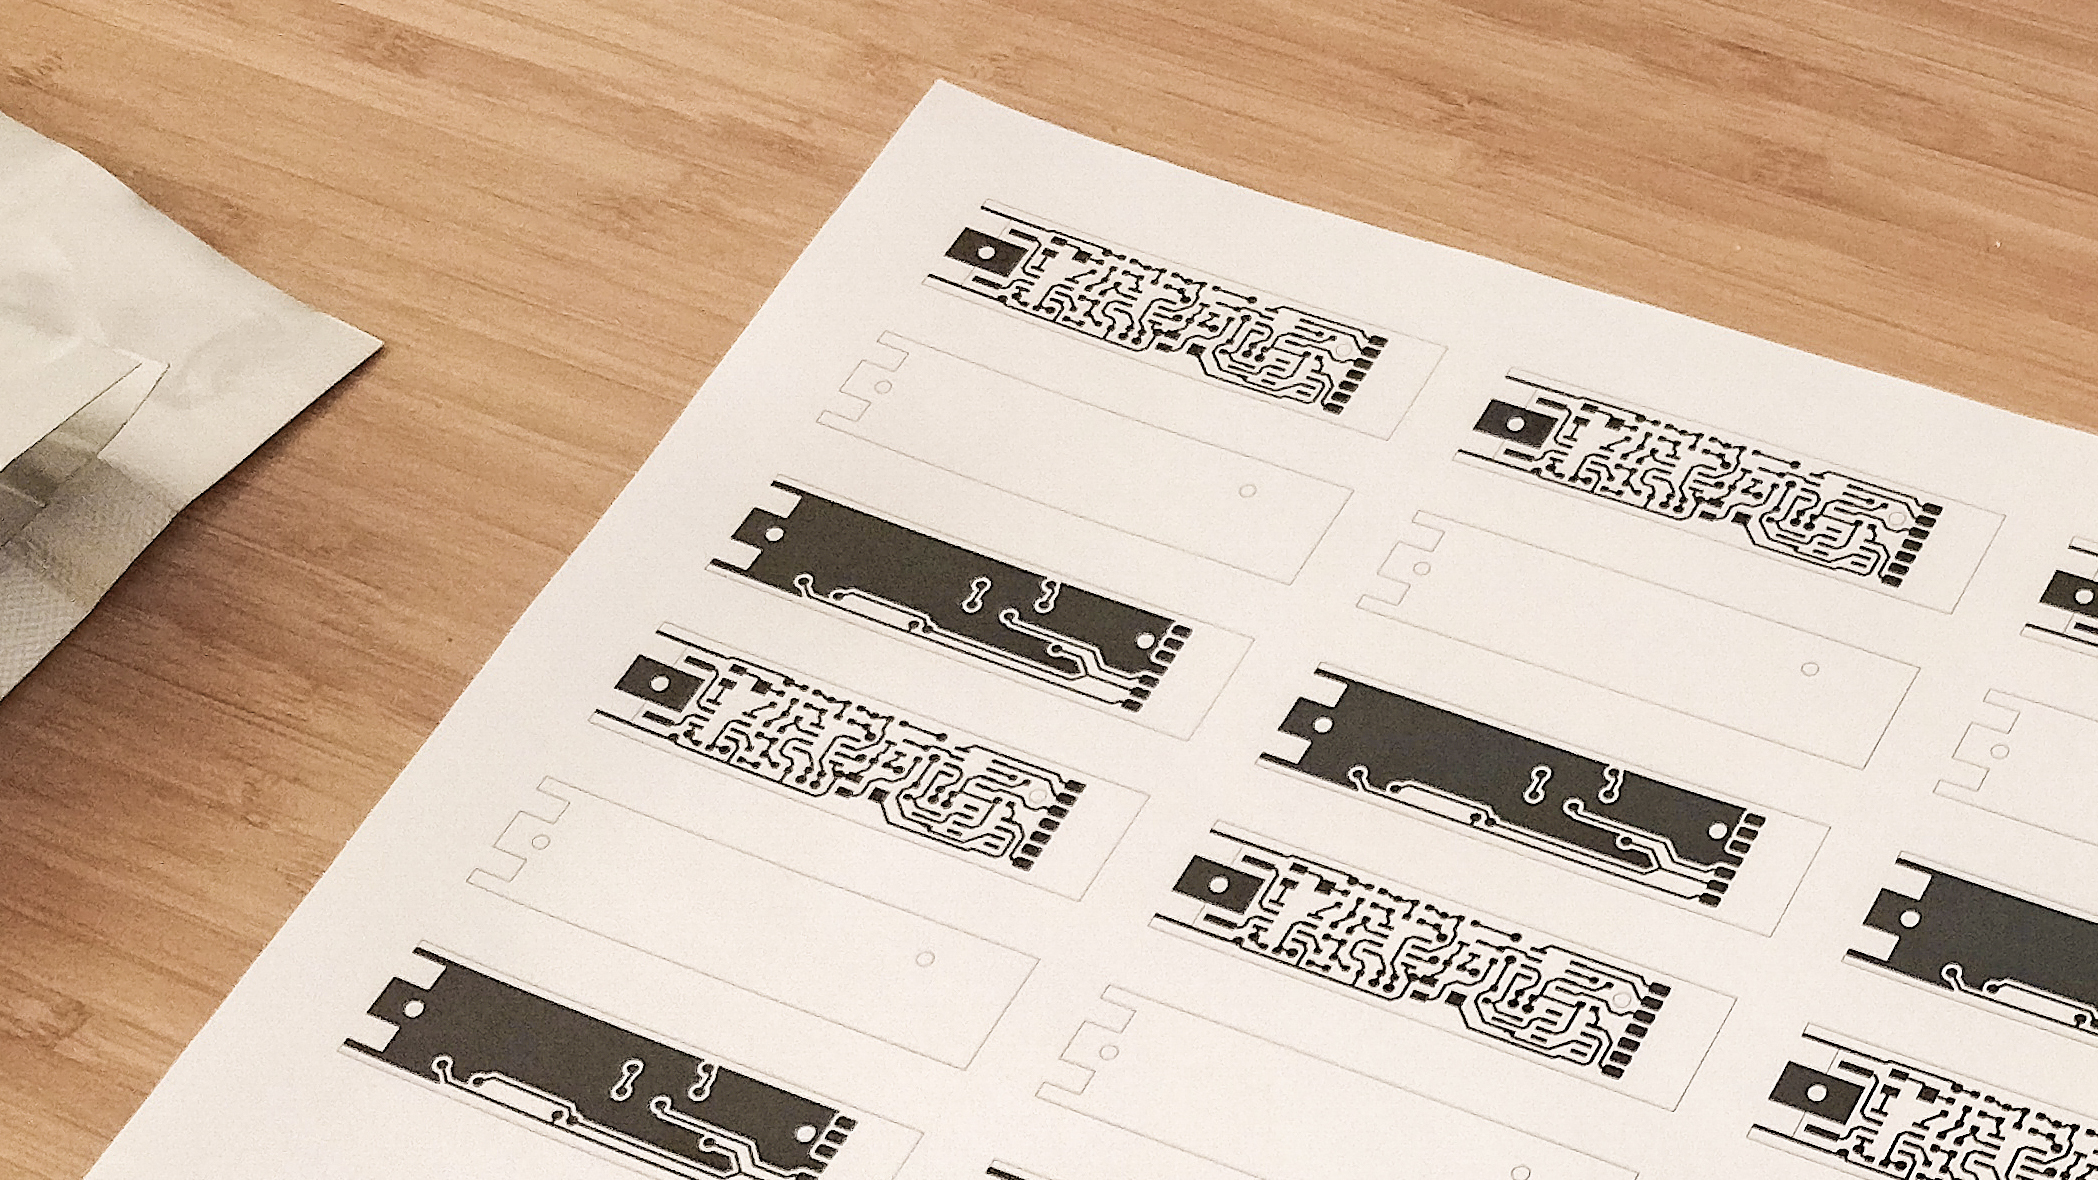
\includegraphics[width=.95\linewidth]{media/album/PSX_20220228_025610.jpg}
        \caption{}
        \label{fig:BuildingHardwarePaperSheet}
    \end{figure}
    I then selected the versions of the circuit that came out best and set them aside to use as masks for chemical etching, and I used the ones that came out worse as a guide to prepare the board blank\footnote{Figure \ref{fig:PhotoPCBCut}}.
    The preparation consisted of drilling holes\footnote{Figure \ref{fig:PhotoPCBDrill}} at certain positions for the vias\footnote{Connections between the layers of the board, which I made simply with a hole and a wire strand} and then cleaning the surface of the board.

    \begin{figure}[H]
        \centering
        \begin{minipage}[H]{.45\linewidth}
            \centering
            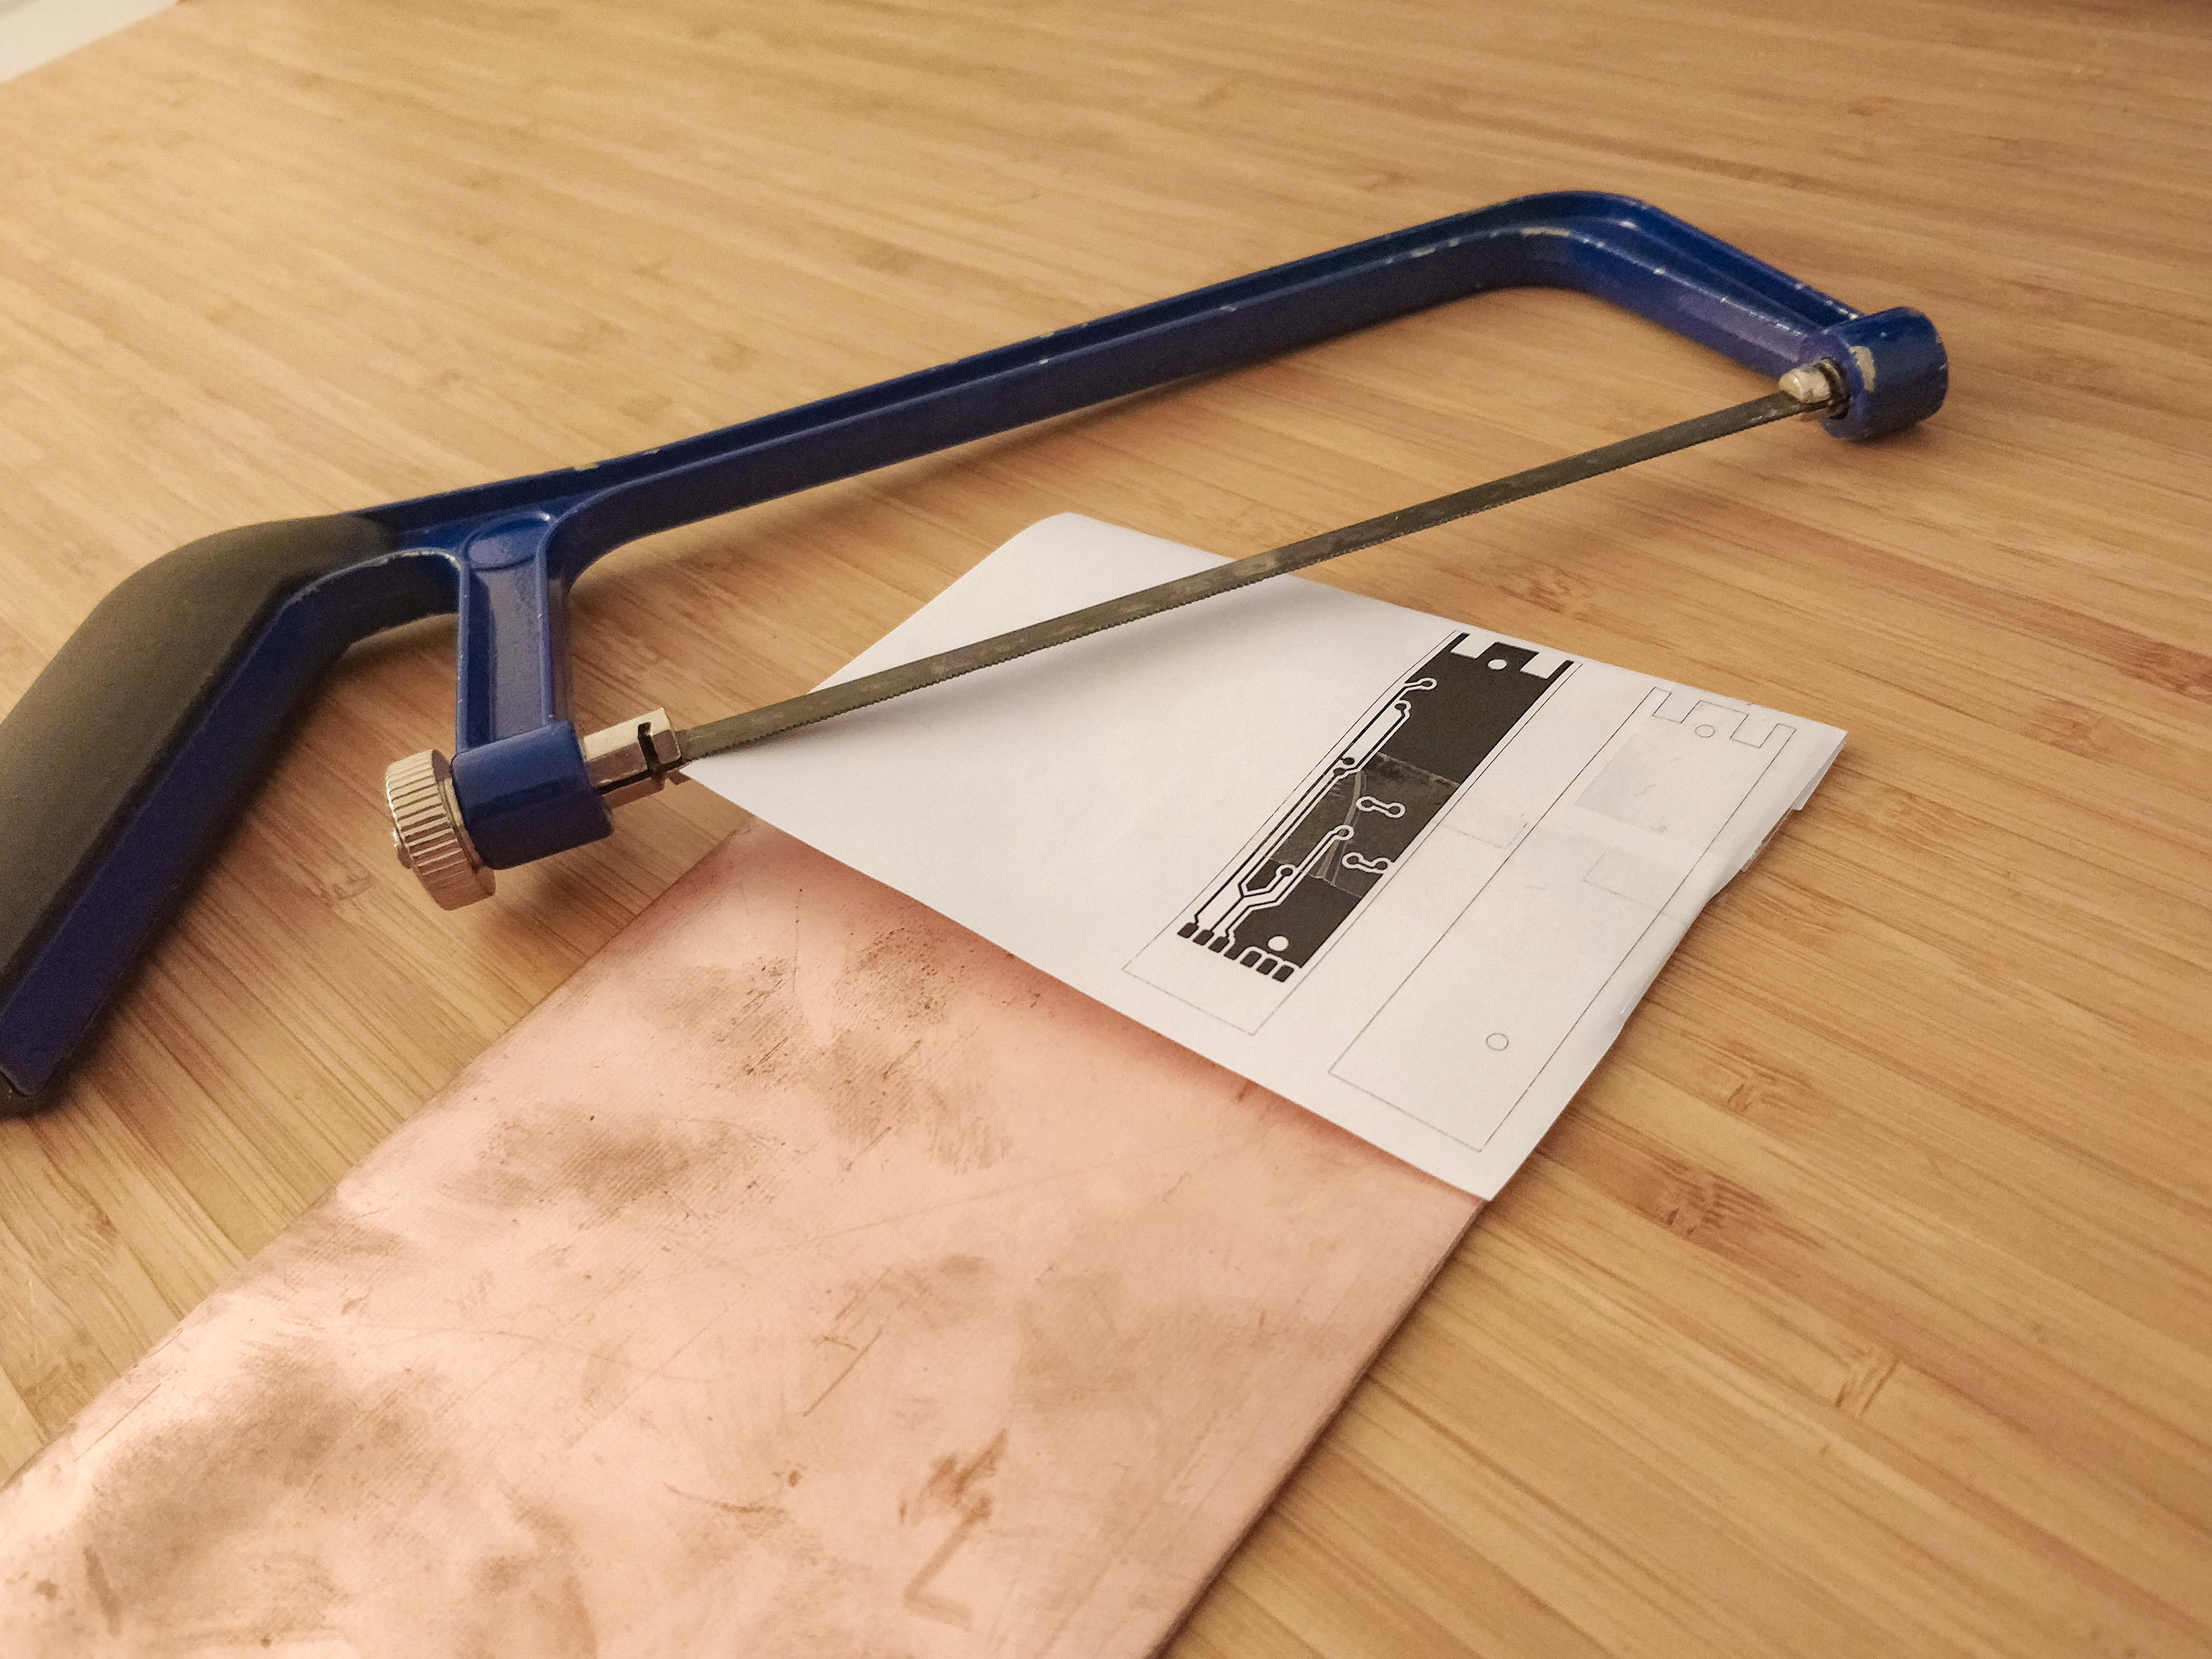
\includegraphics[width=\linewidth]{media/album/PSX_20220228_025933.jpg}
            \caption{}
            \label{fig:PhotoPCBCut}
        \end{minipage}
        \hspace{.04\linewidth}
        \begin{minipage}[H]{.45\linewidth}
            \centering
            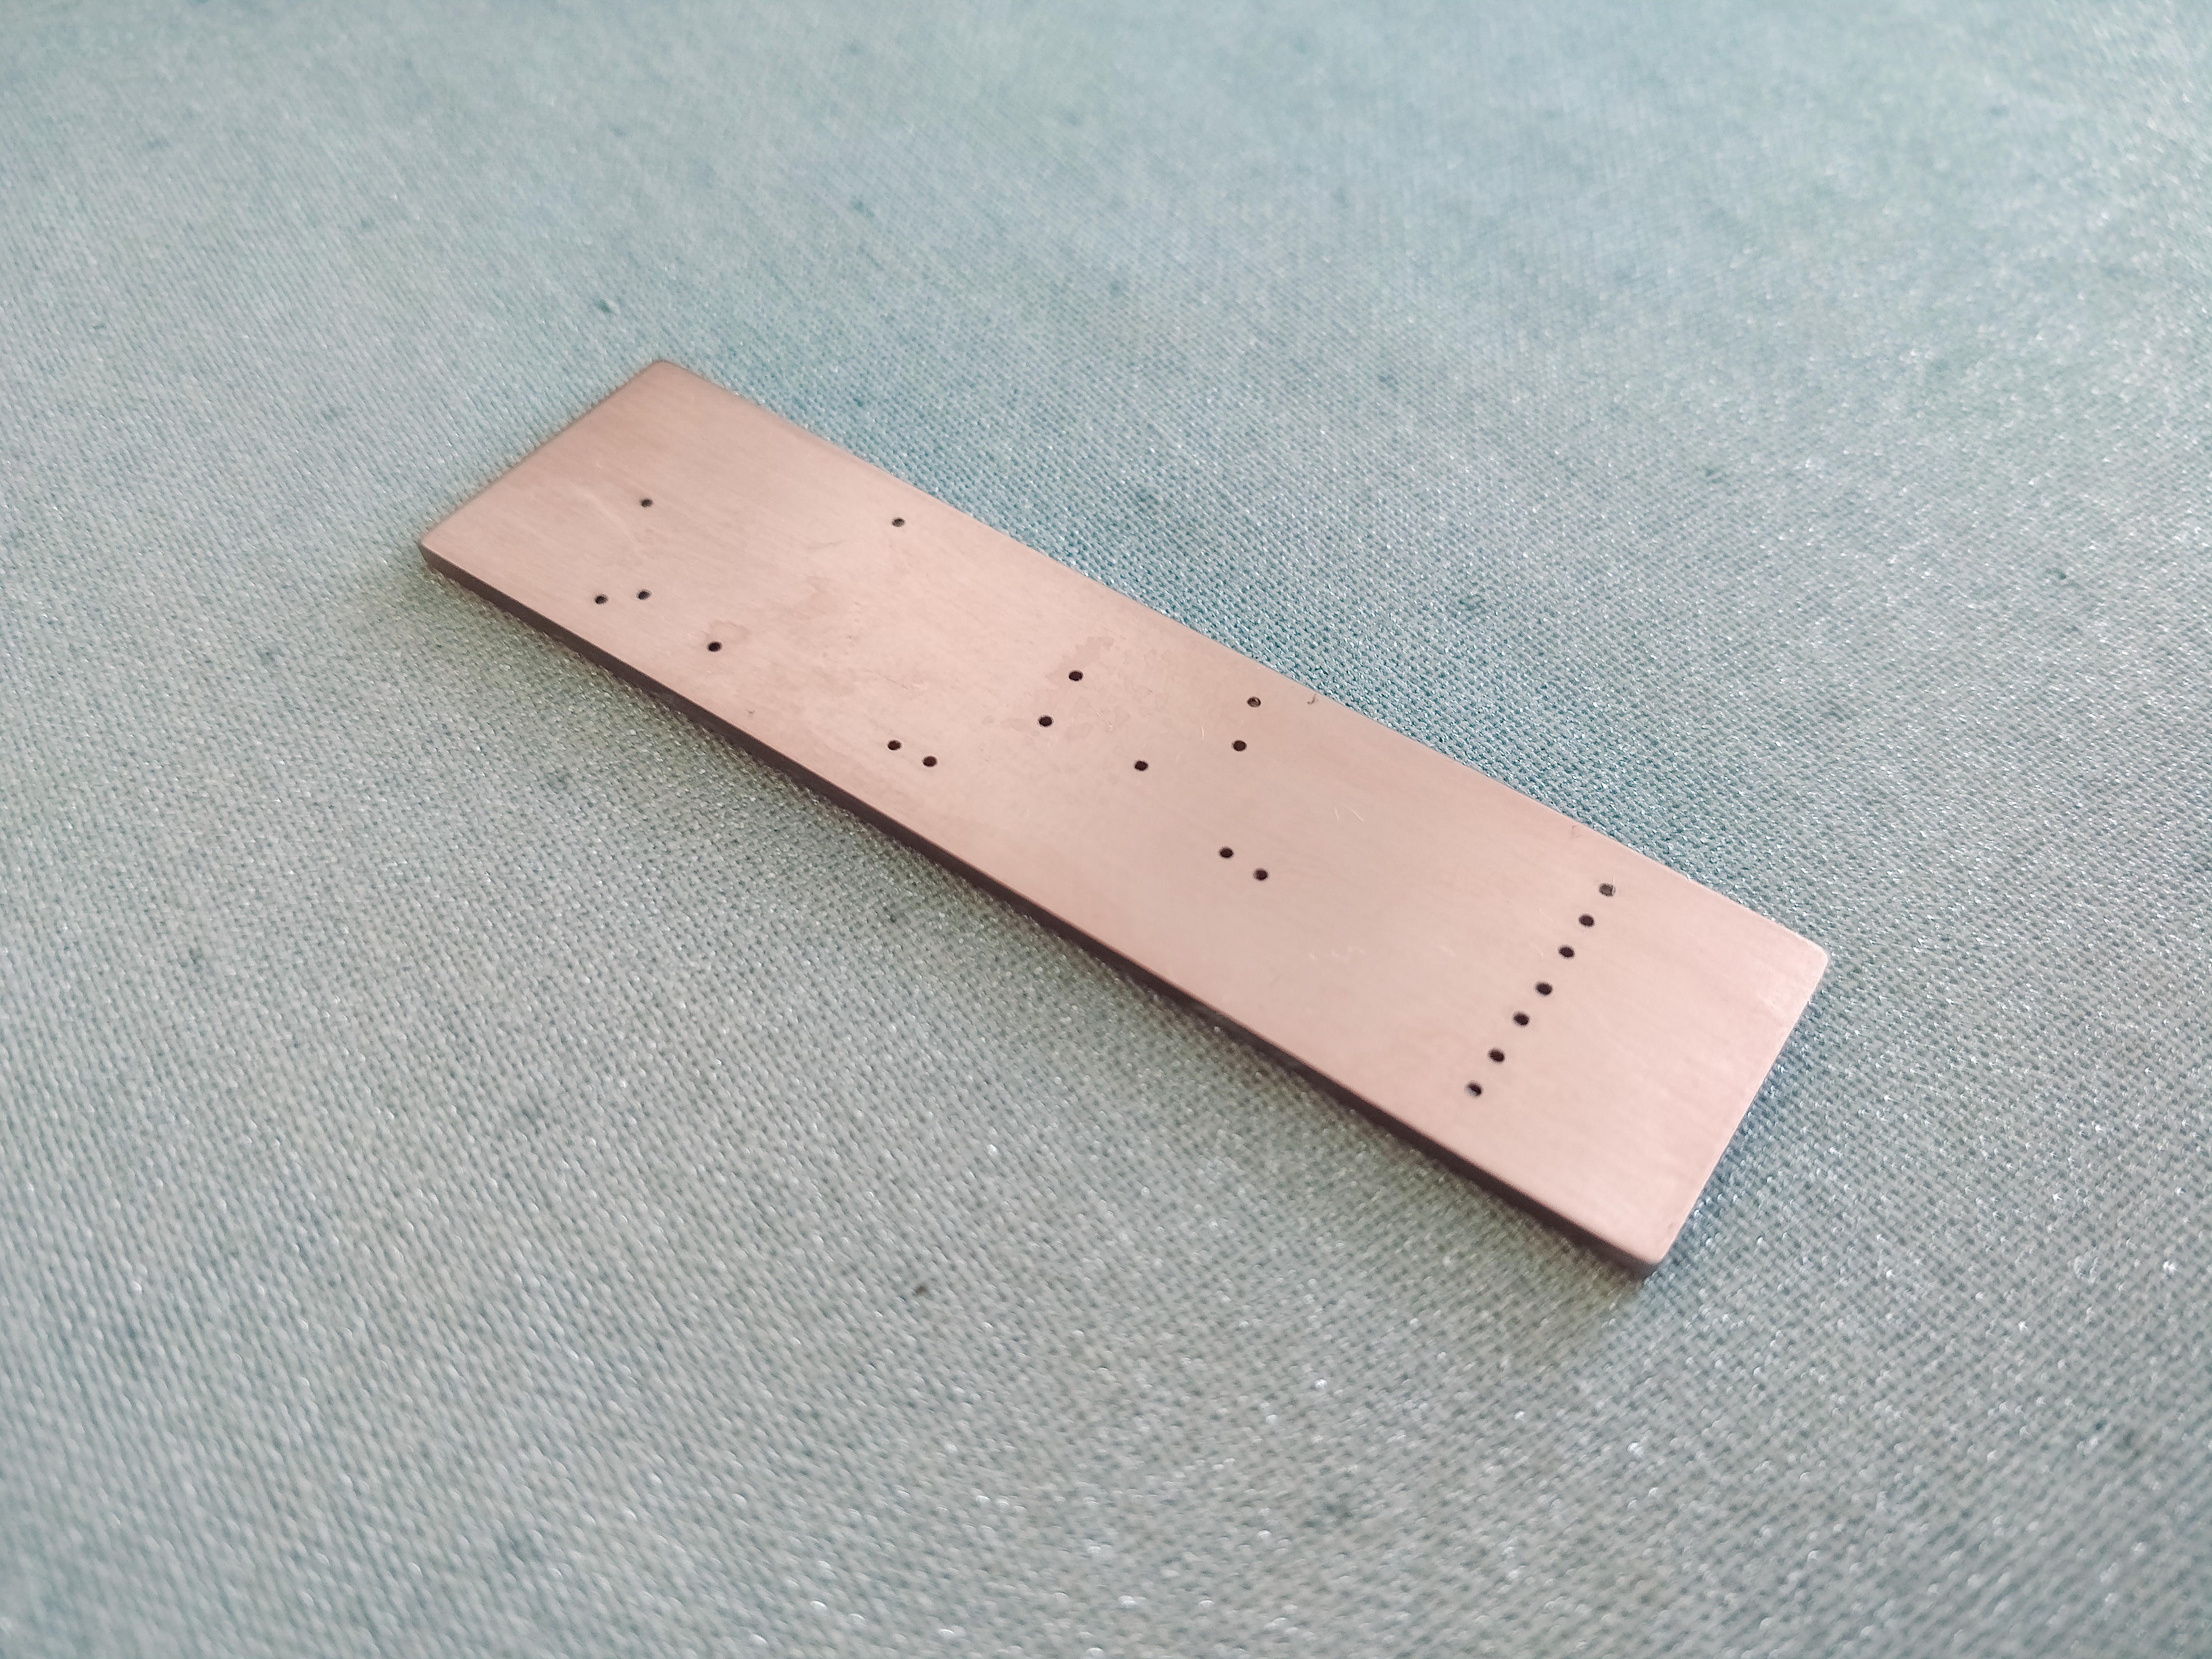
\includegraphics[width=\linewidth]{media/album/PSX_20220228_174045.jpg}
            \caption{}
            \label{fig:PhotoPCBDrill}
        \end{minipage}
    \end{figure}
    \clearpage

    After preparing a solution\footnote{Figures \ref{fig:PhotoSolutionPrep}, \ref{fig:PhotoSolution}} of 40\%\emph{(m/m)}\footnote{I decided to replicate a commercial board-etching solution \parenciteit{p1}{FECL3:Datasheet}} FeCl3\footnote{The solute must be added little by little to the solution while checking that its temperature does not exceed $55^{\circ}C$ \parenciteit{p2}{FECL3:Datasheet}, because the process is exothermic} I started the etching process in a well-ventilated place\footnote{In the reaction with copper, $Cl_2$ gas can form: $FeCl_3 + Cu \Rightarrow CuCl + FeCl_2$ and then $FeCl_2 + Cu \Rightarrow CuFe + Cl_2$}.

    \begin{figure}[H]
        \centering
        \begin{minipage}[H]{.525\linewidth}
            \centering
            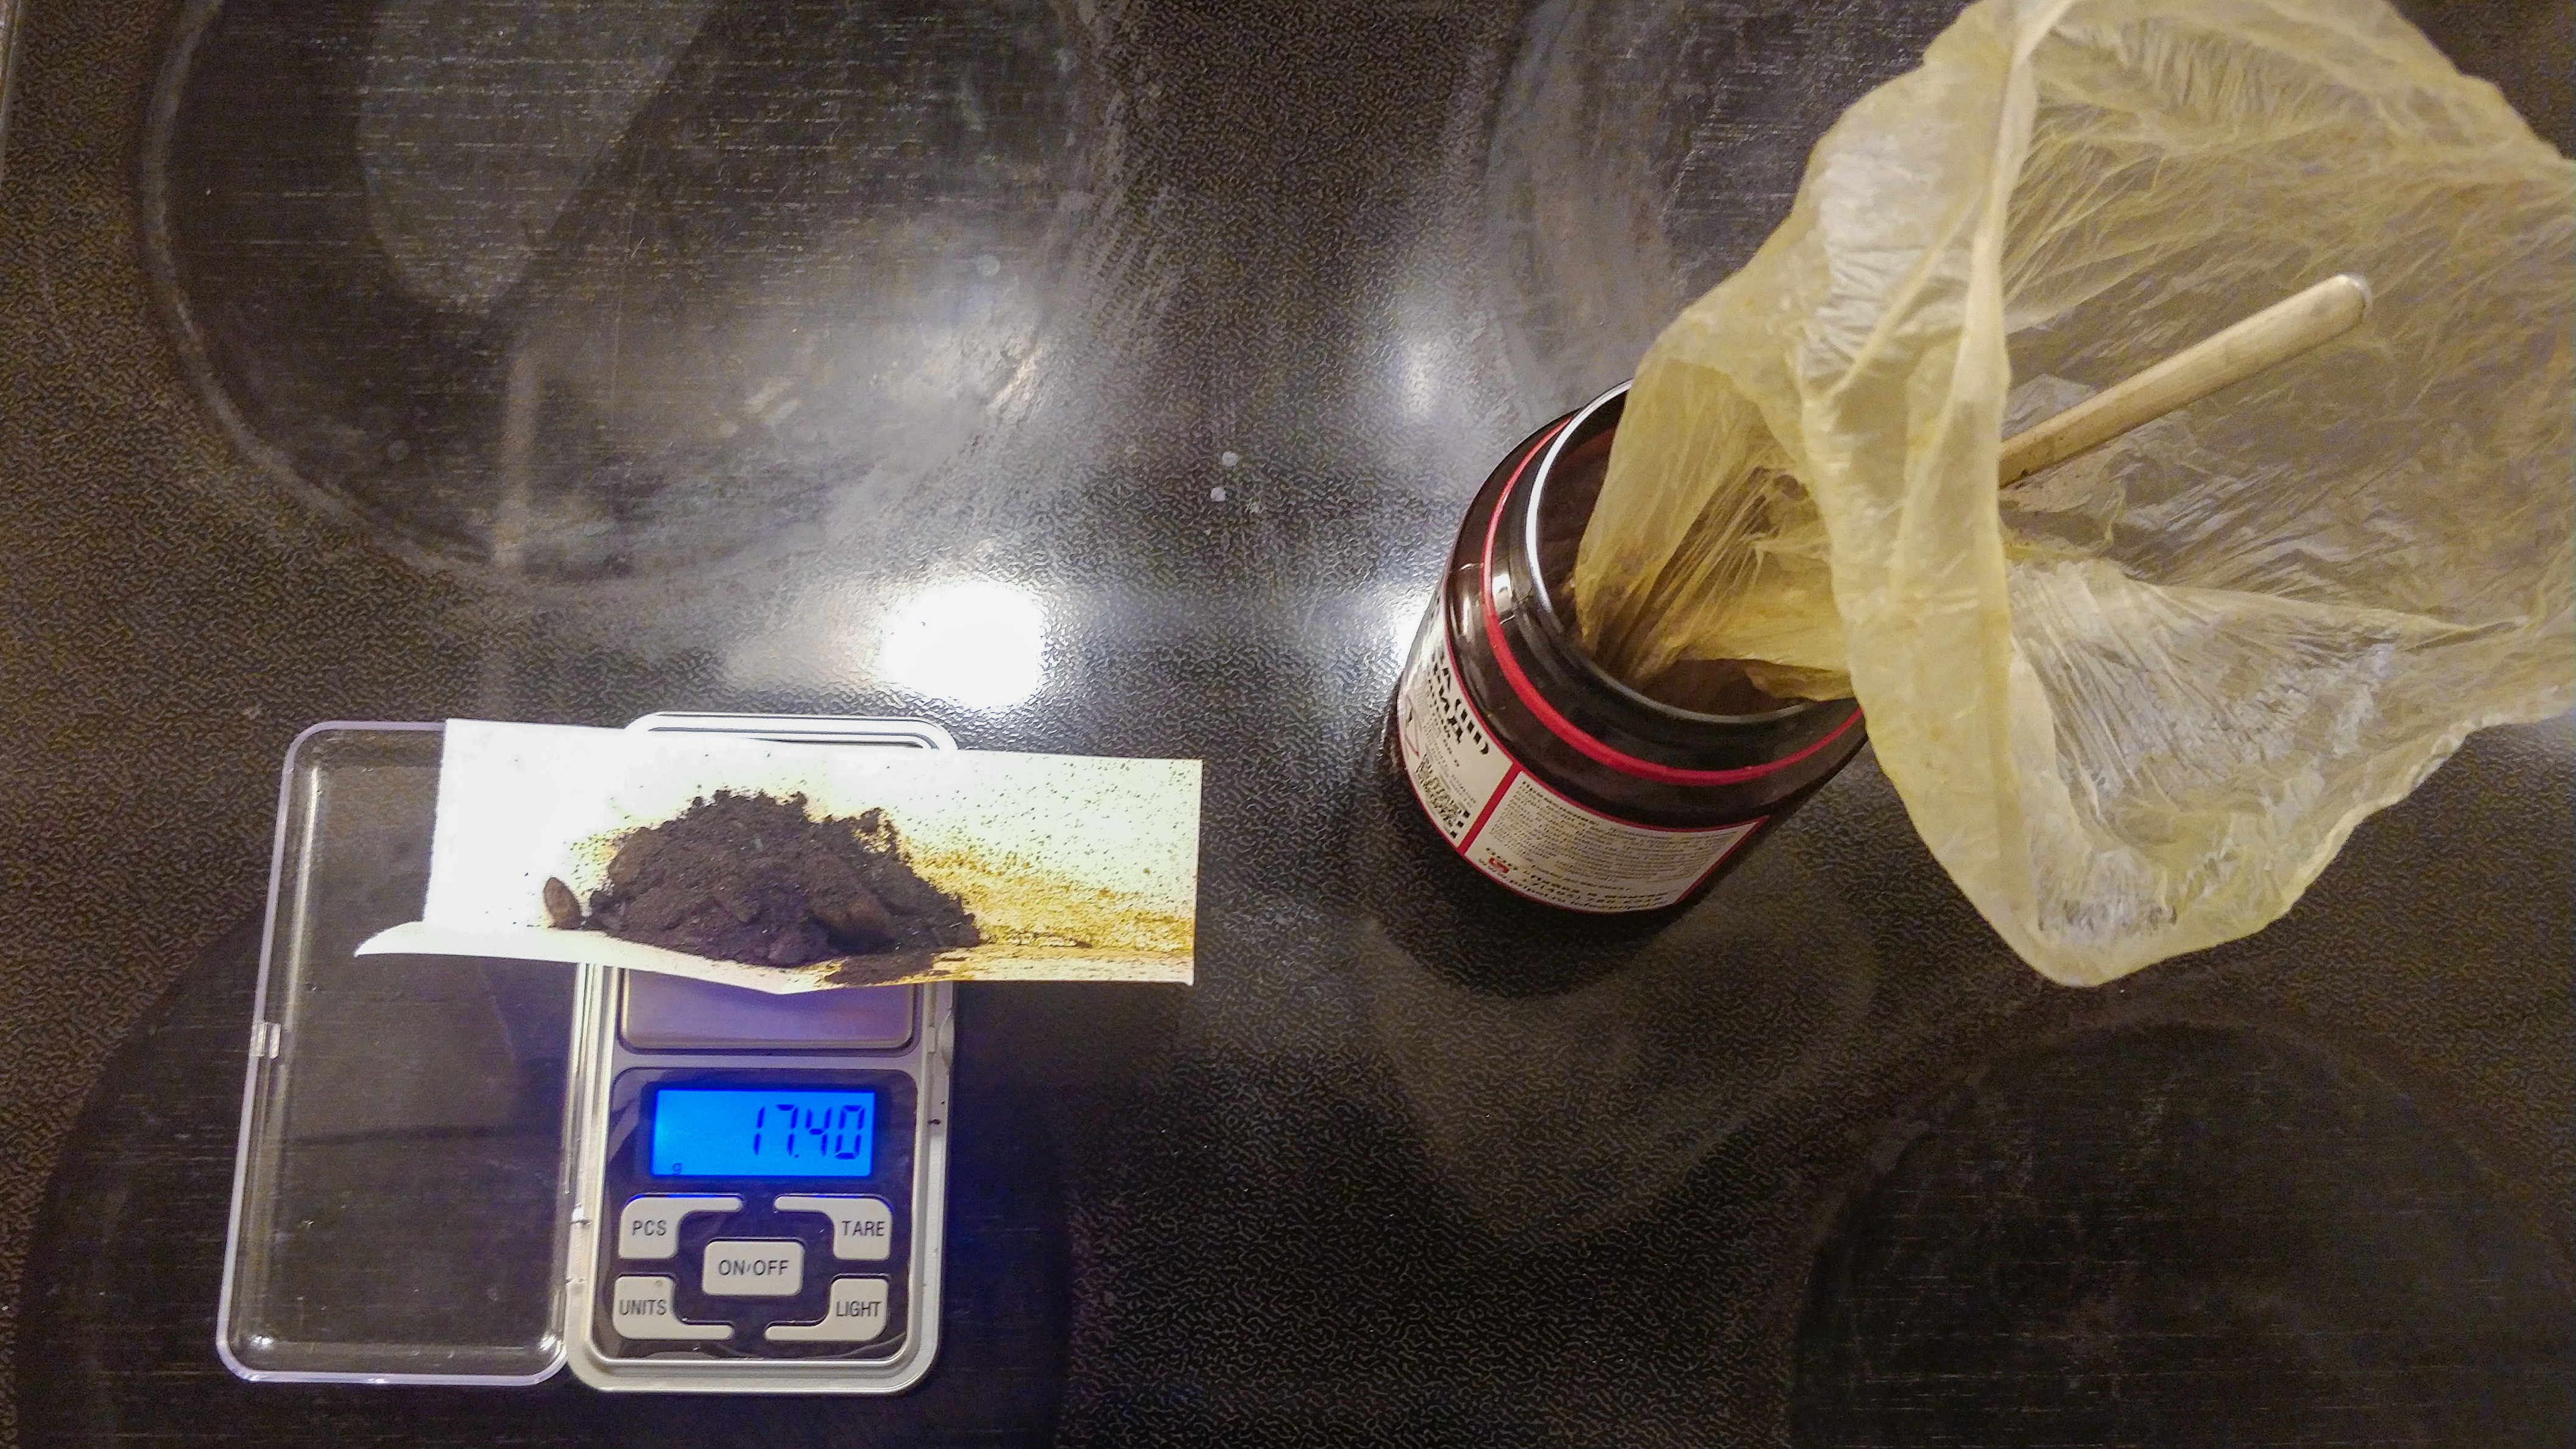
\includegraphics[width=\linewidth]{media/album/PSX_20220228_160724.jpg}
            \caption{}
            \label{fig:PhotoSolutionPrep}
        \end{minipage}
        \hspace{.04\linewidth}
        \begin{minipage}[H]{.394\linewidth}
            \centering
            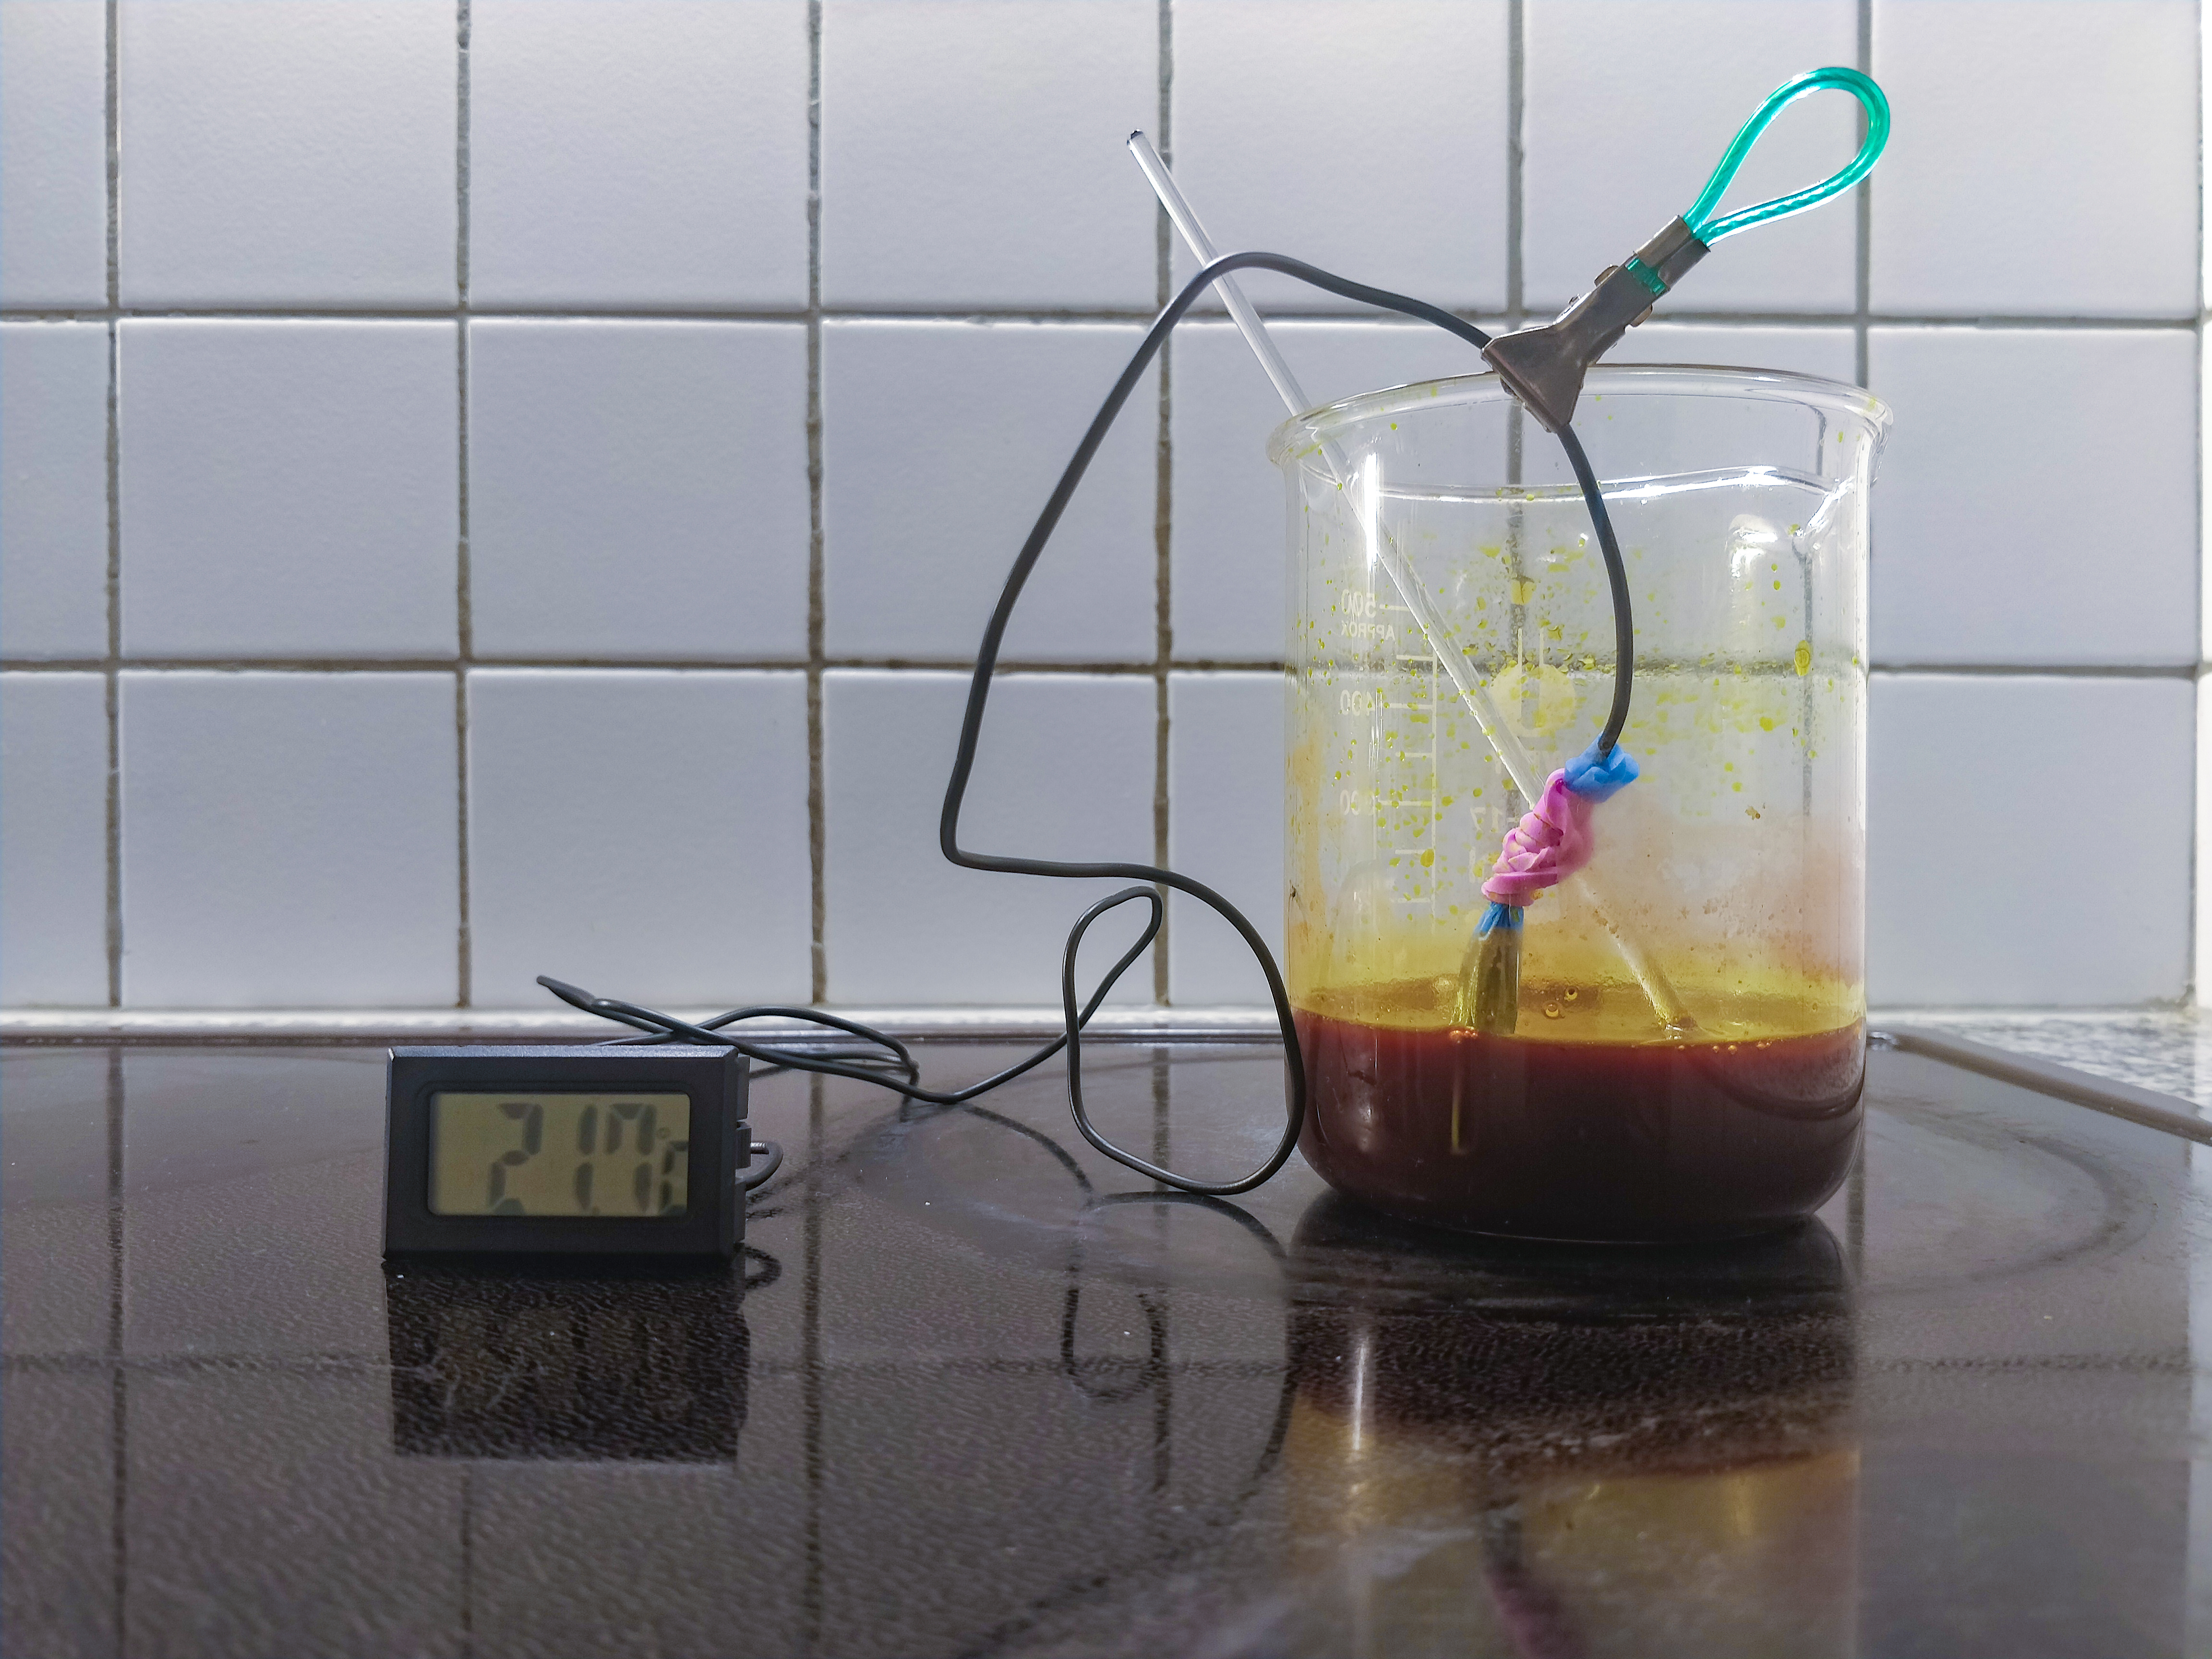
\includegraphics[width=\linewidth]{media/album/PSX_20220301_014813.jpg}
            \caption{}
            \label{fig:PhotoSolution}
        \end{minipage}
    \end{figure}


    The process follows the technique used for all DIY\footnote{Do-It-Yourself} boards: as already said, one has to print the circuit on a piece of paper, lay it with the printed side on the clean surface of the prepared board and bond the toner by temporarily applying heat\footnote{Normally a clothes iron is used}\:\footnote{Figure \ref{fig:PhotoPCBIron}}.
    Then the sheet with the circuit must be removed\footnote{Figure\ref{fig:PhotoPCBWash}} carefully.
    The most effective method is to wet the sheet and rub it away little by little with something rough but soft, such as a sponge.
    Having completely cleaned the circuit, I was left with toner traces bonded to the surface of the board.
    These will protect against the etching solution: the exposed parts will react with the solution and be eaten away over time, while the covered parts will remain attached.

    \begin{figure}[H]
        \centering
        \begin{minipage}[H]{.331\linewidth}
            \centering
            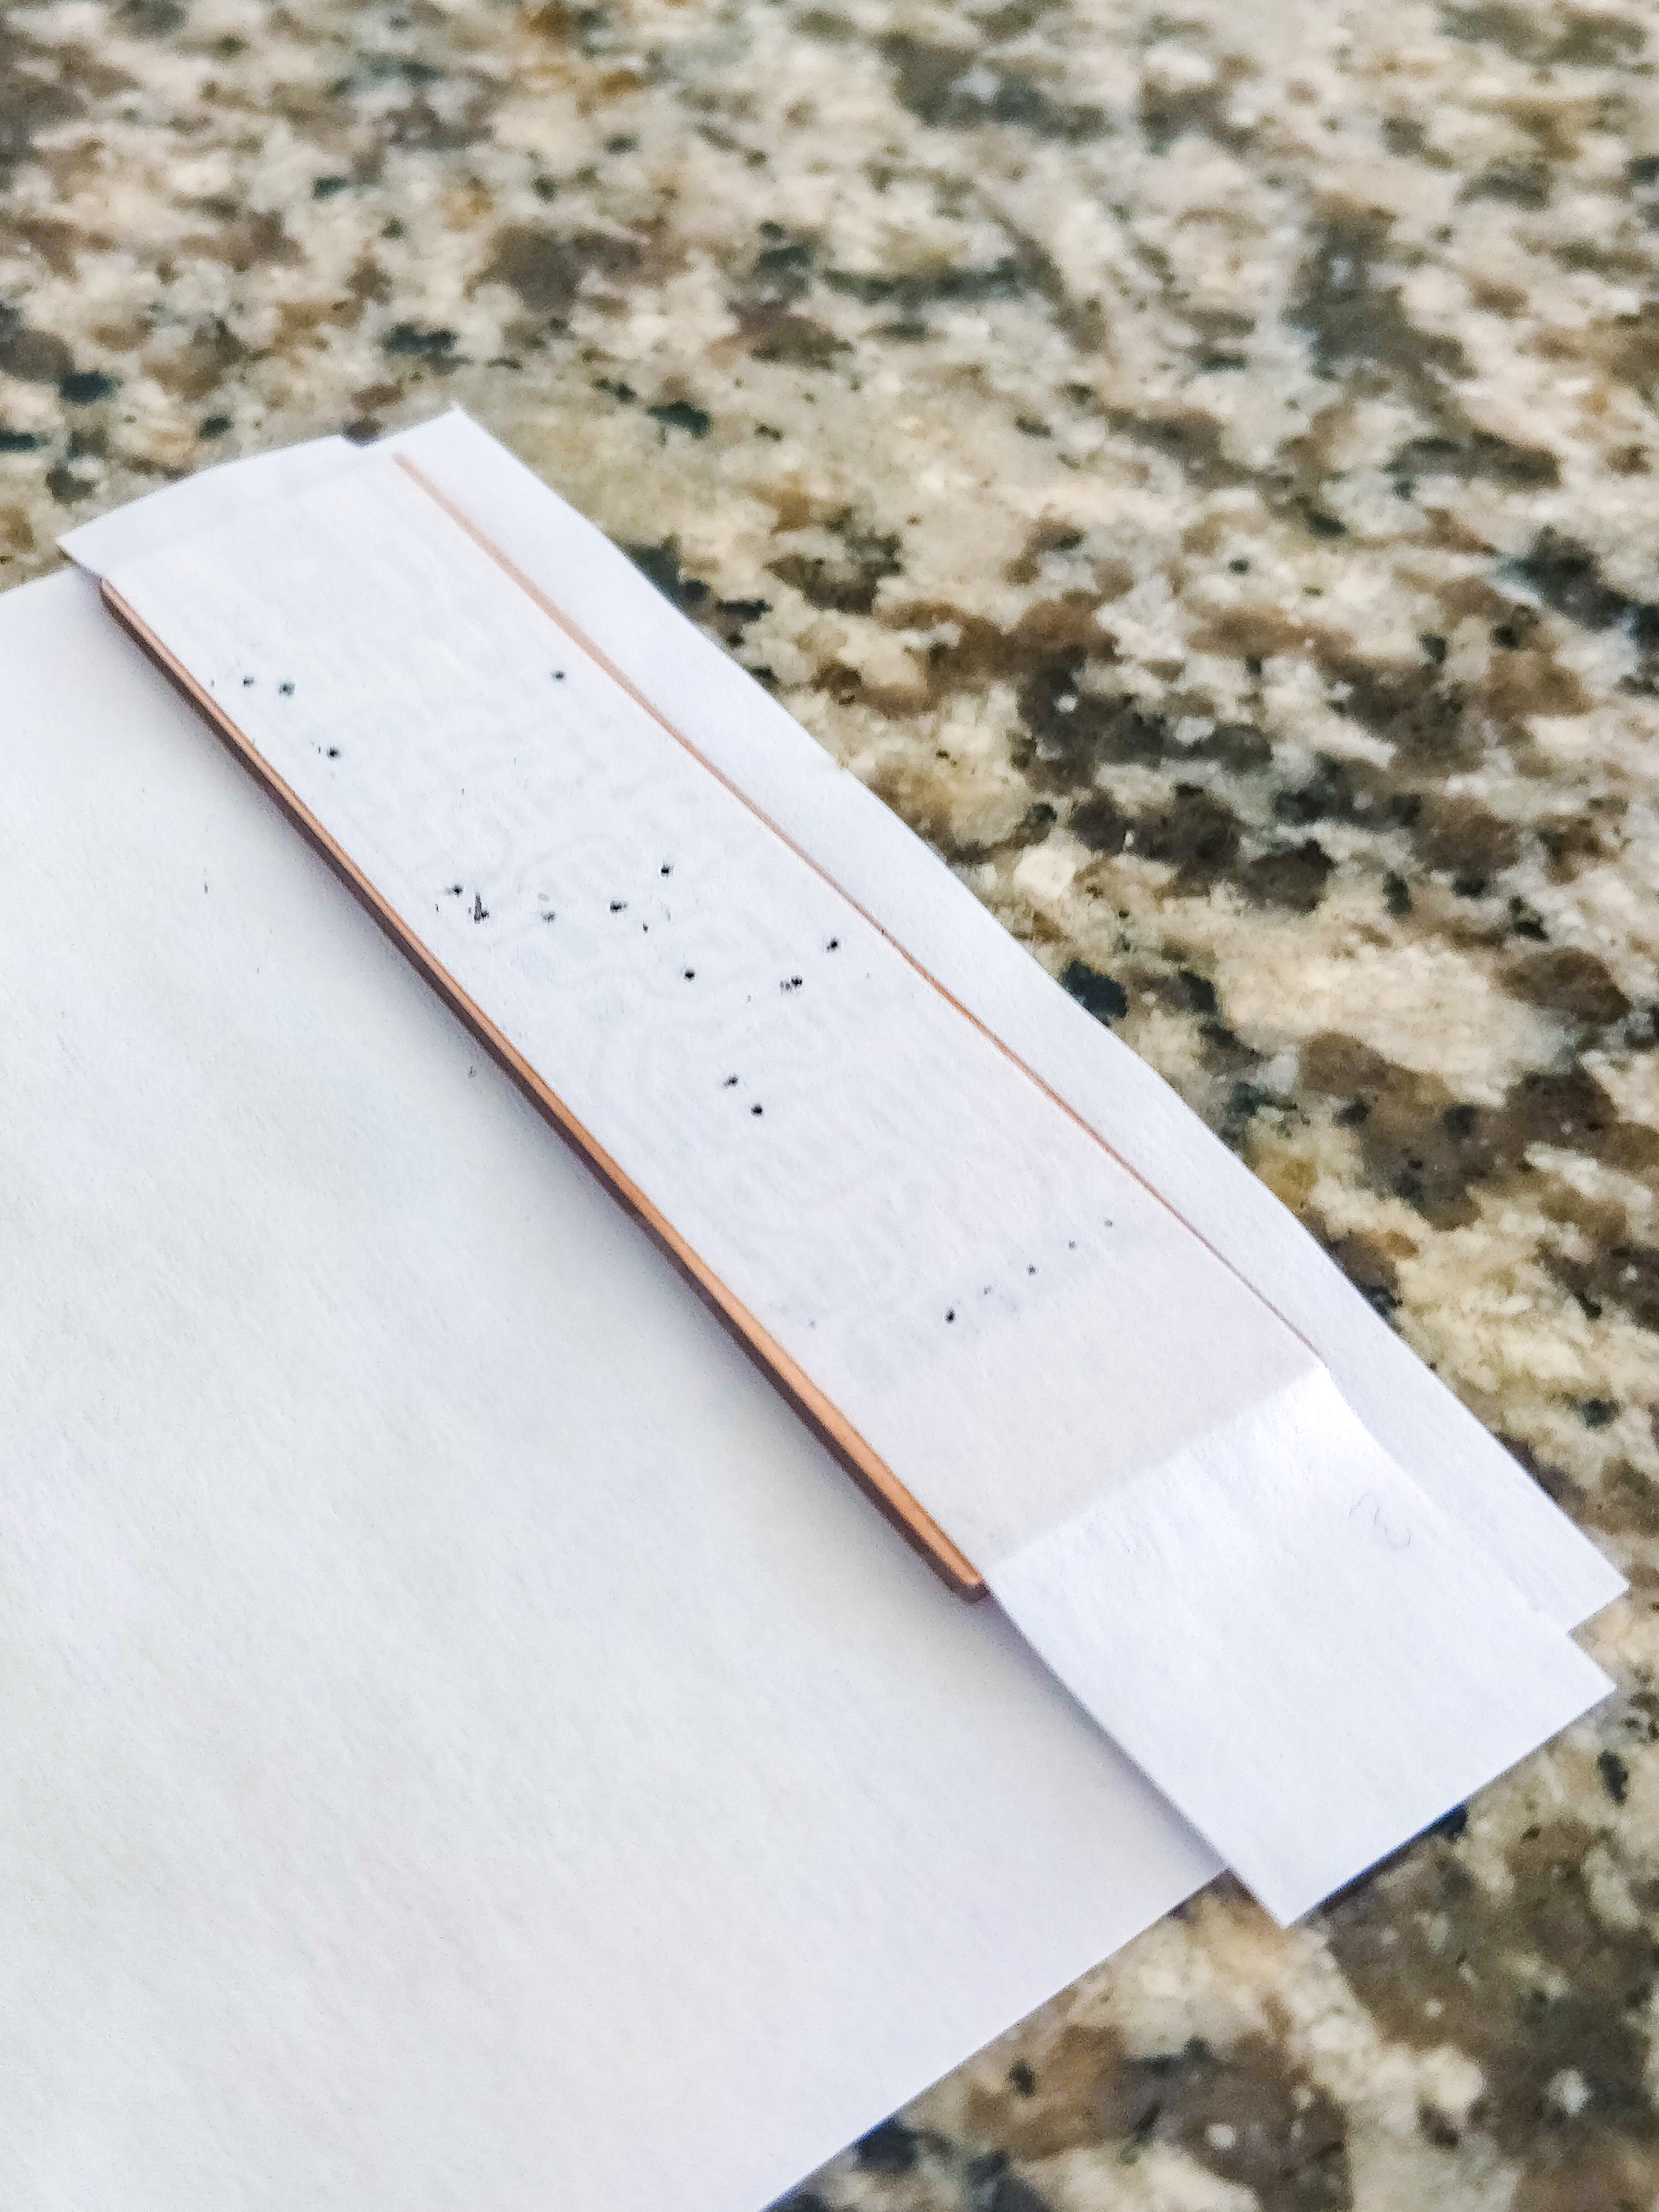
\includegraphics[width=\linewidth]{media/album/PSX_20220228_020336.jpg}
            \caption{}
            \label{fig:PhotoPCBIron}
        \end{minipage}
        \hspace{.04\linewidth}
        \begin{minipage}[H]{.5888\linewidth}
            \centering
            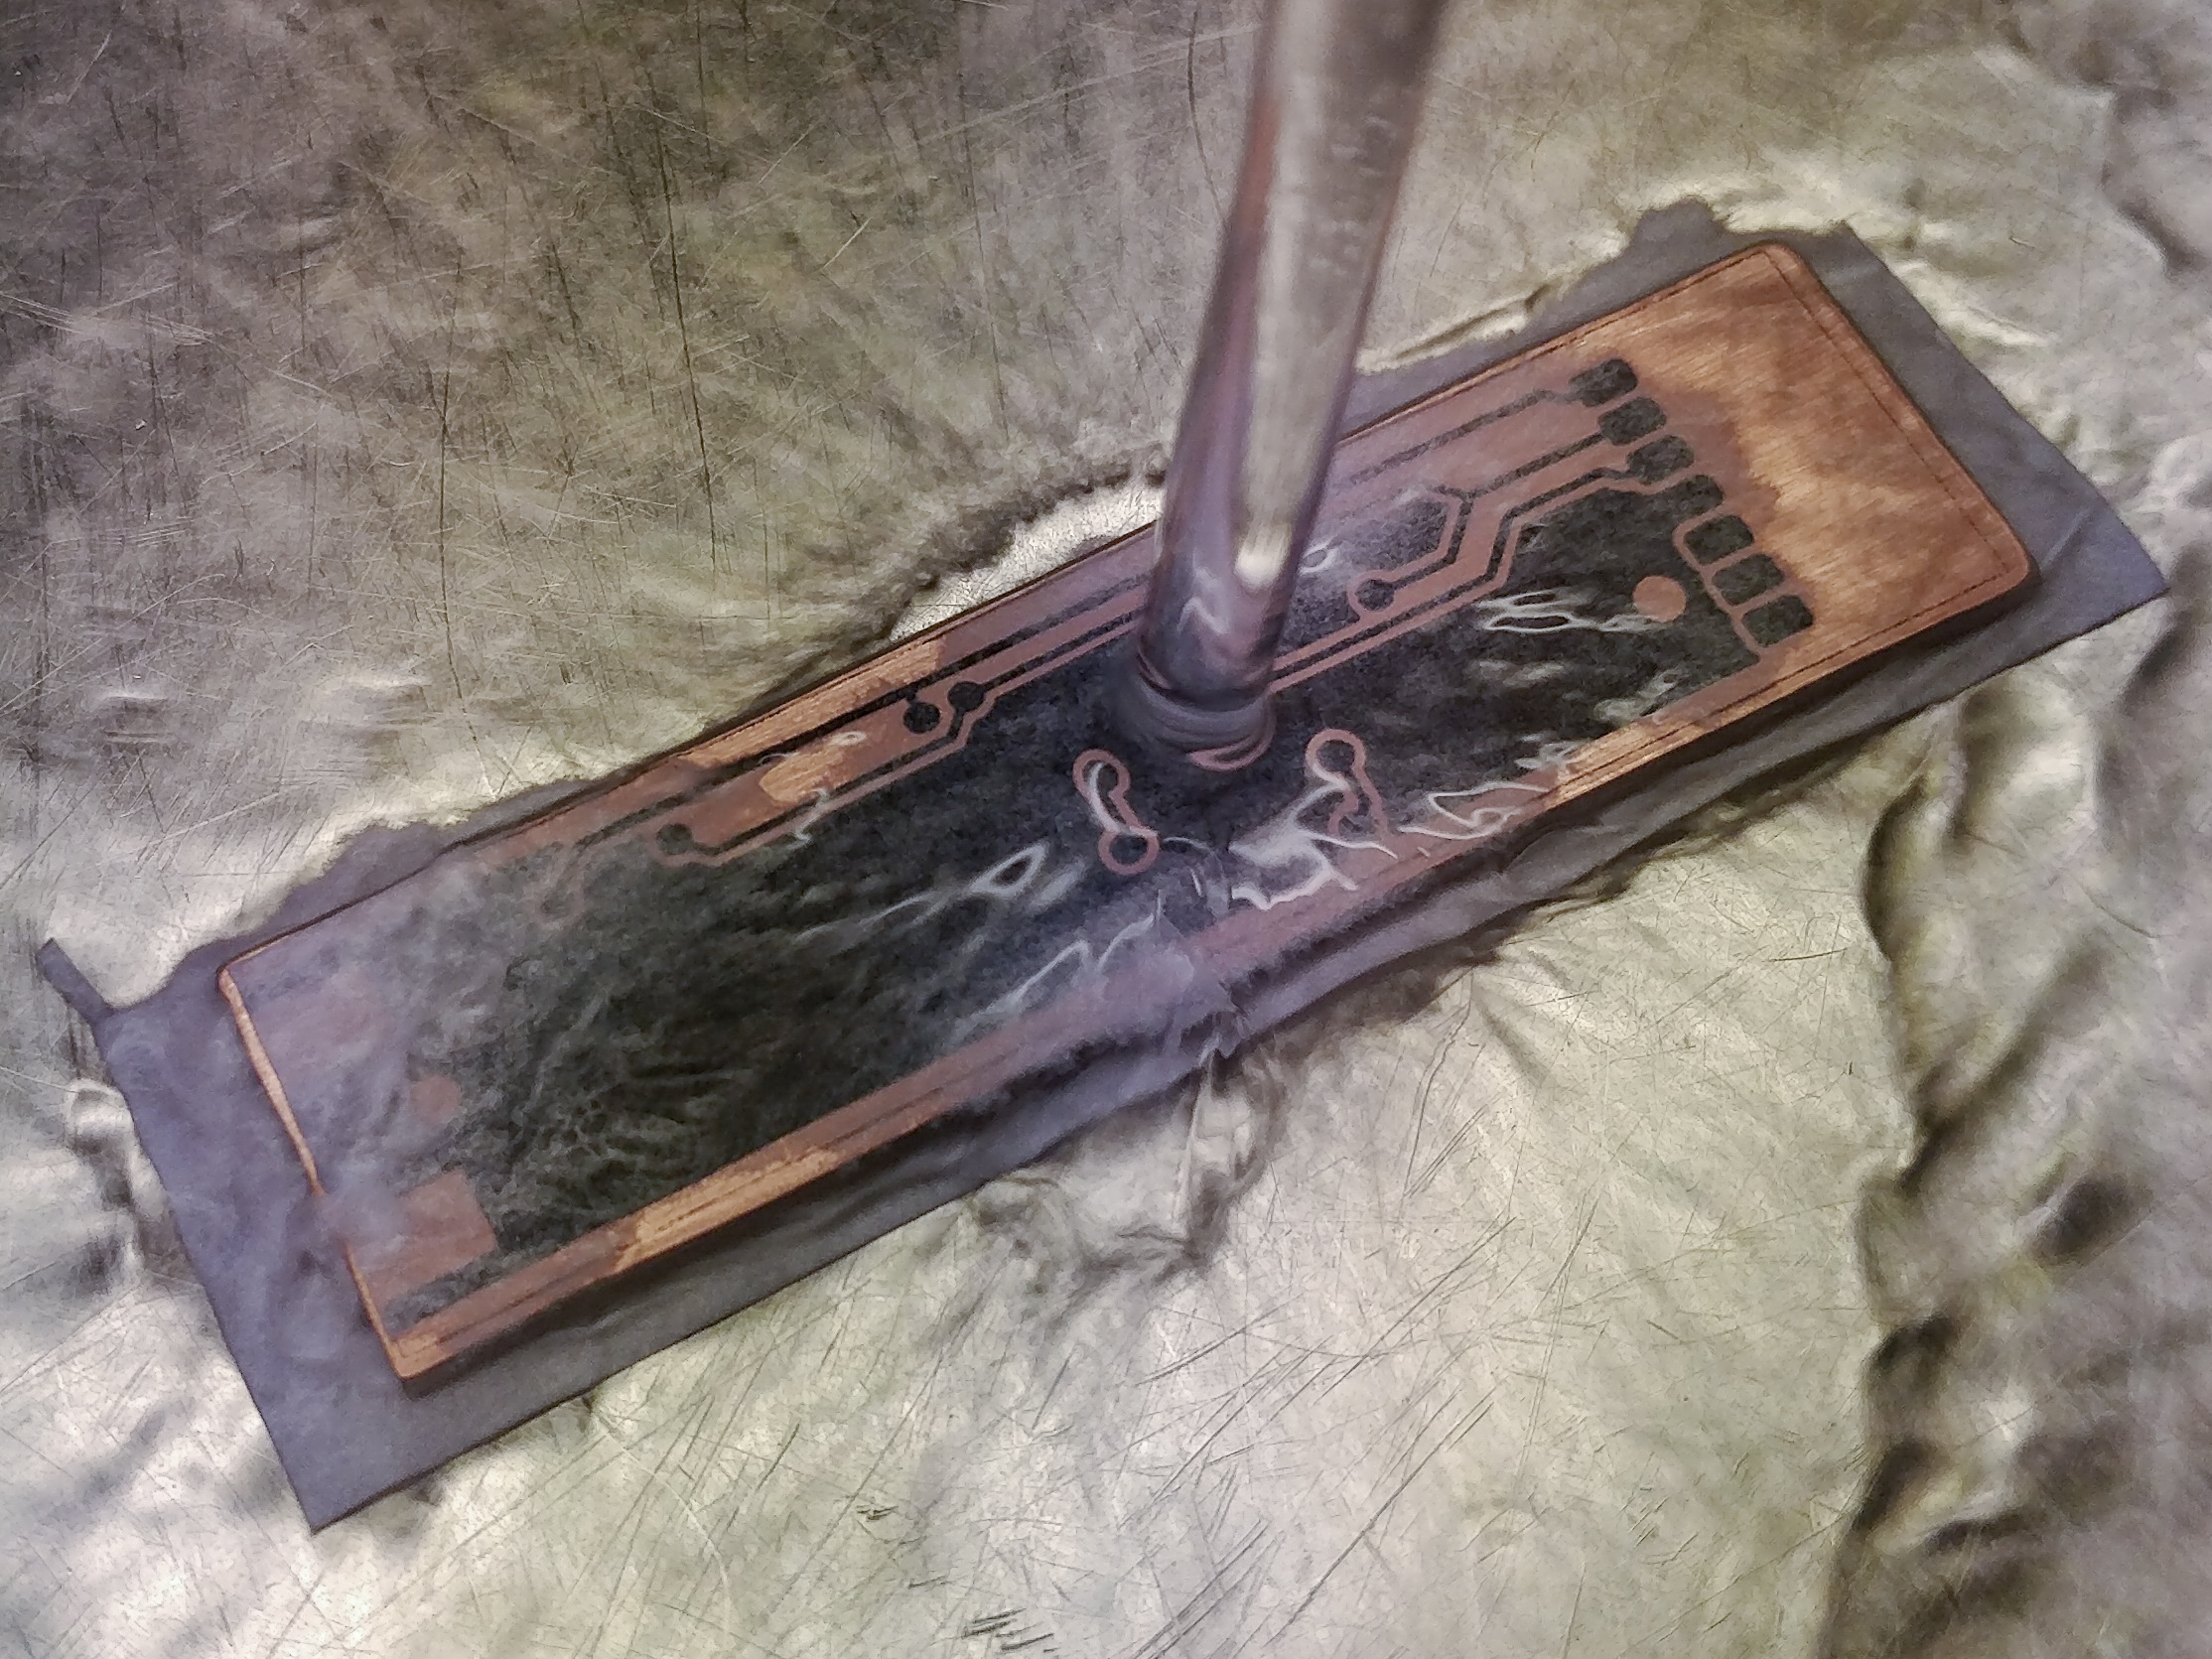
\includegraphics[width=\linewidth]{media/album/PSX_20220301_034705.jpg}
            \caption{}
            \label{fig:PhotoPCBWash}
        \end{minipage}
    \end{figure}
    \clearpage

    The circuit stayed\footnote{Figures \ref{fig:PhotoPCBPrepare1}, \ref{fig:PhotoPCBPrepare2}, \ref{fig:PhotoPCBPrepare3}, \ref{fig:PhotoPCBPrepareDone}} in the solution for about 10 minutes, while the copper dissolved little by little.
    Moreover, the solution can be warmed a little to speed up the process \emph{(Again without exceeding $55^{\circ}C$)}
    \begin{figure}[H]
        \centering
        \begin{minipage}[H]{.45\linewidth}
            \centering
            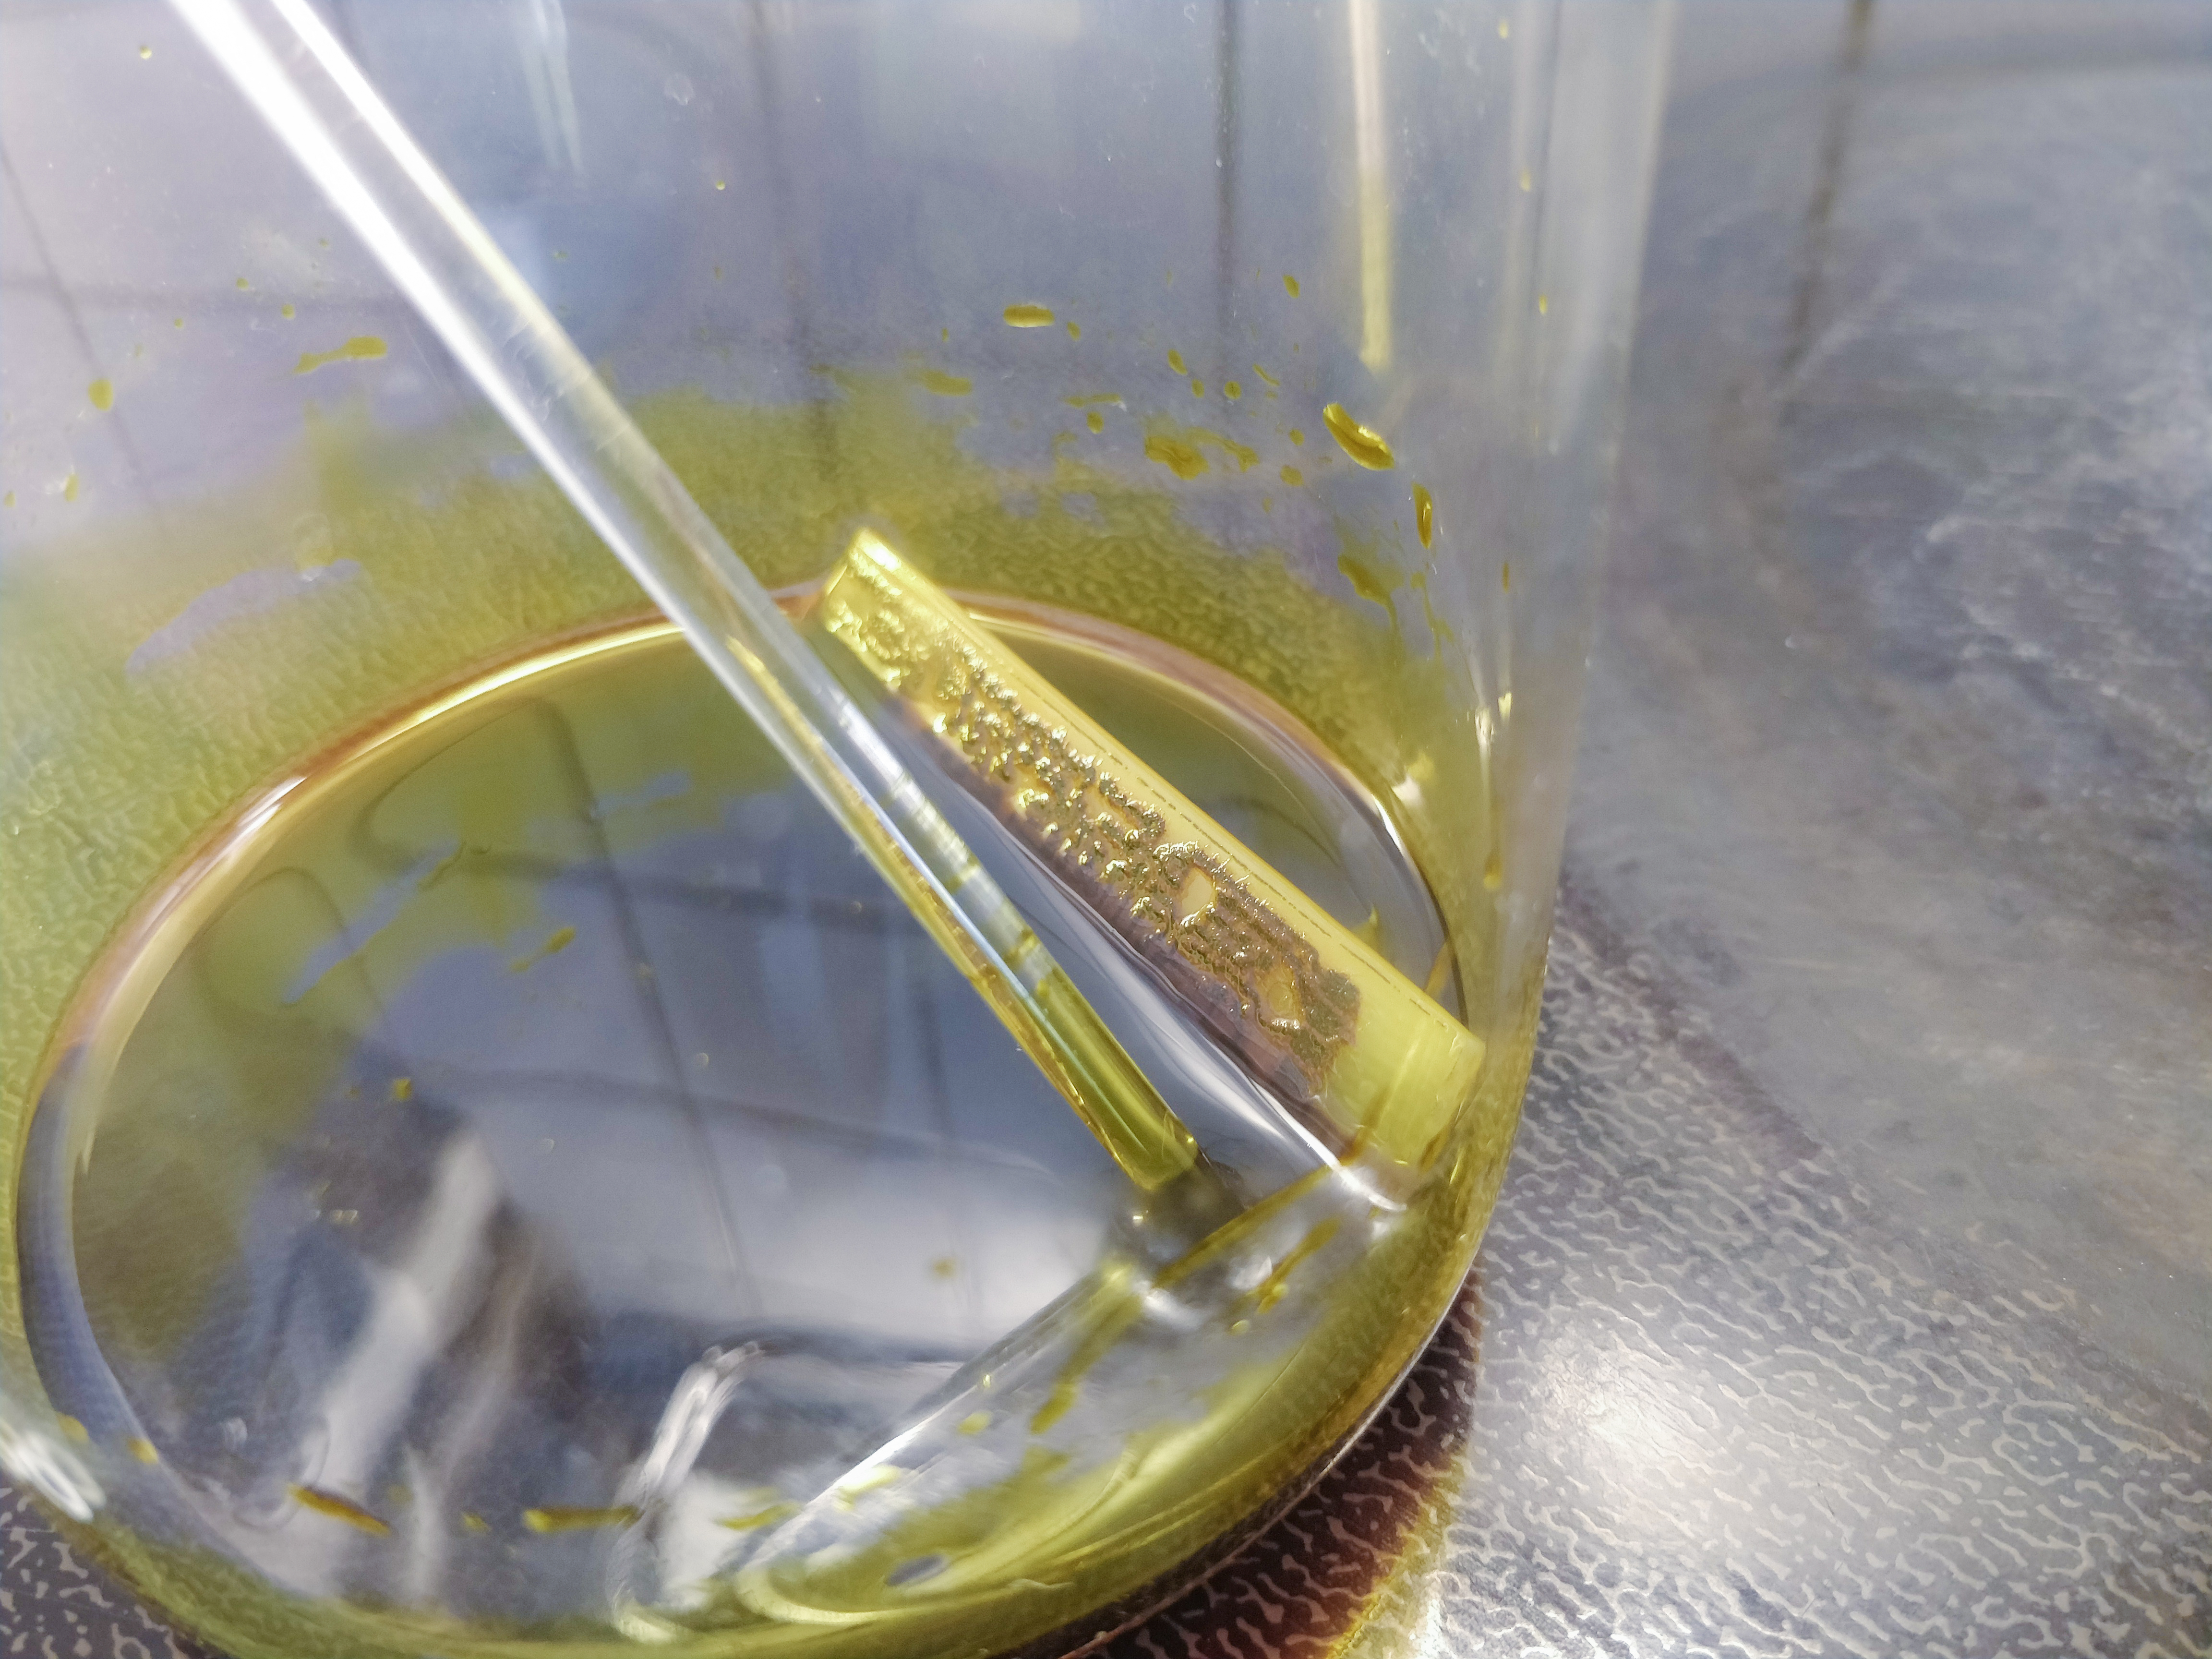
\includegraphics[width=\linewidth]{media/album/PSX_20220301_014718.jpg}
            \caption{}
            \label{fig:PhotoPCBPrepare1}
        \end{minipage}
        \hspace{.04\linewidth}
        \begin{minipage}[H]{.45\linewidth}
            \centering
            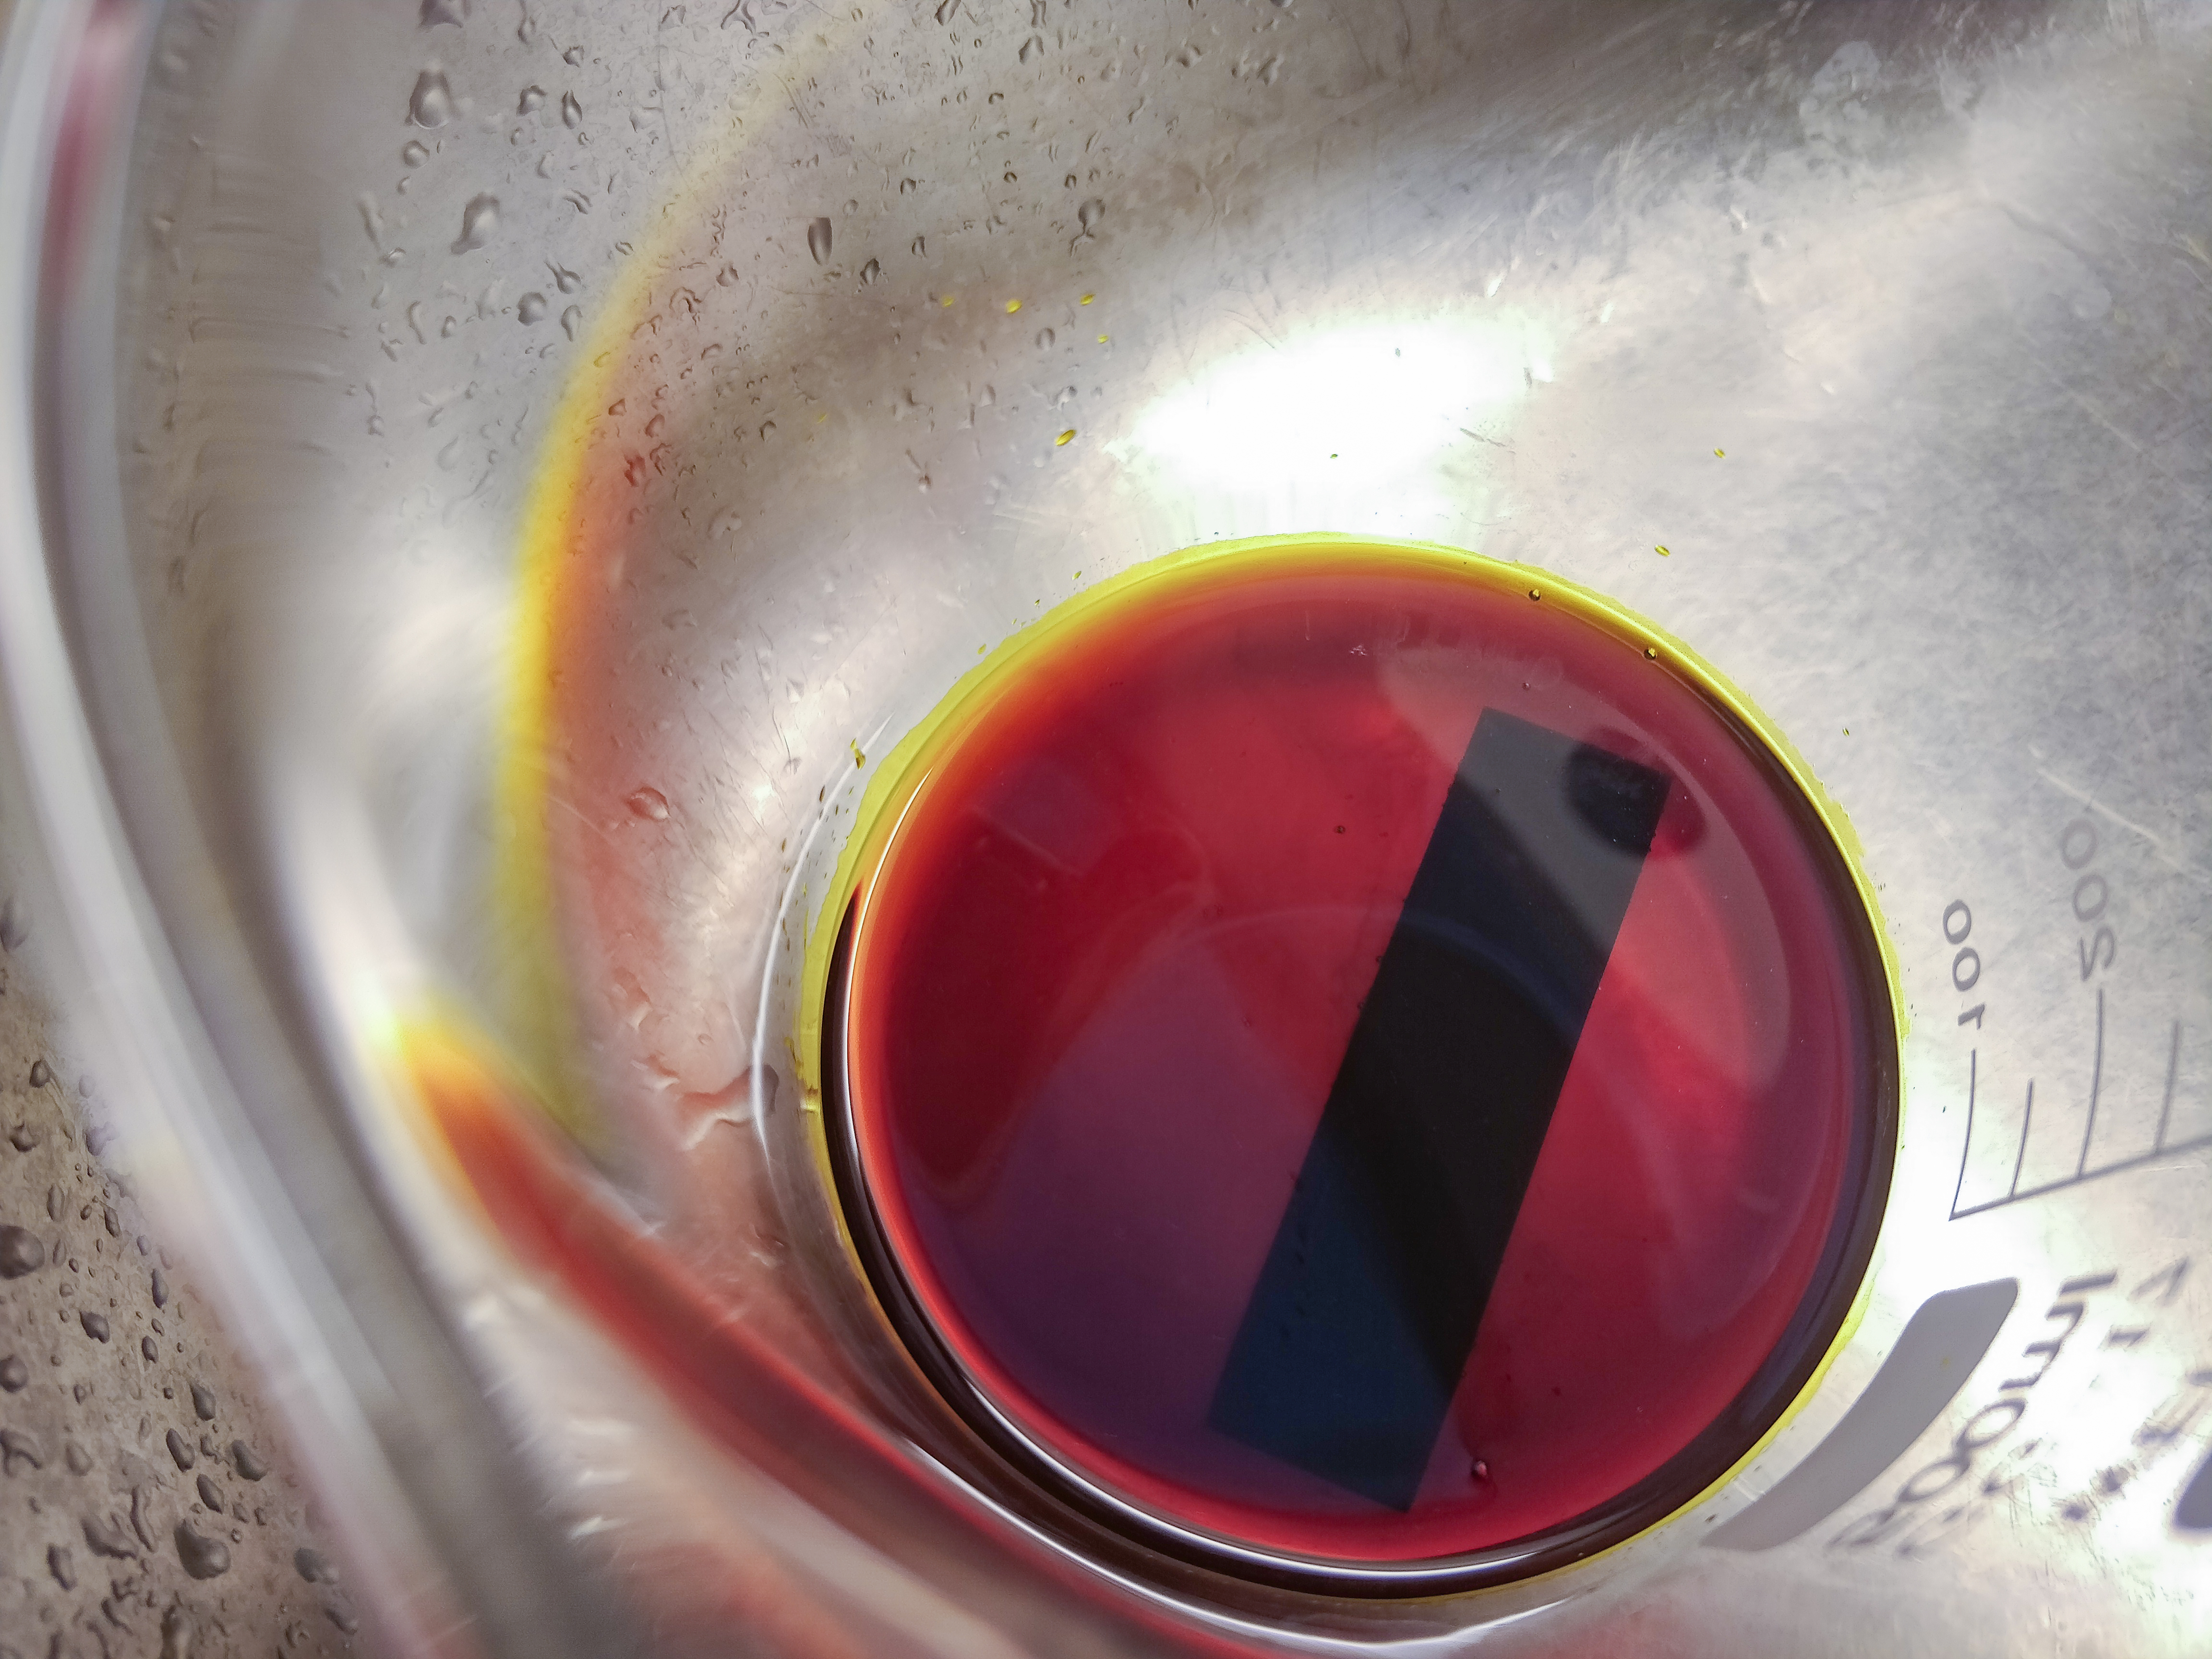
\includegraphics[width=\linewidth]{media/album/PSX_20220301_014557.jpg}
            \caption{}
            \label{fig:PhotoPCBPrepare2}
        \end{minipage}
        \\
        \vspace*{.01\linewidth}
        \begin{minipage}[H]{.95\linewidth}
            \centering
            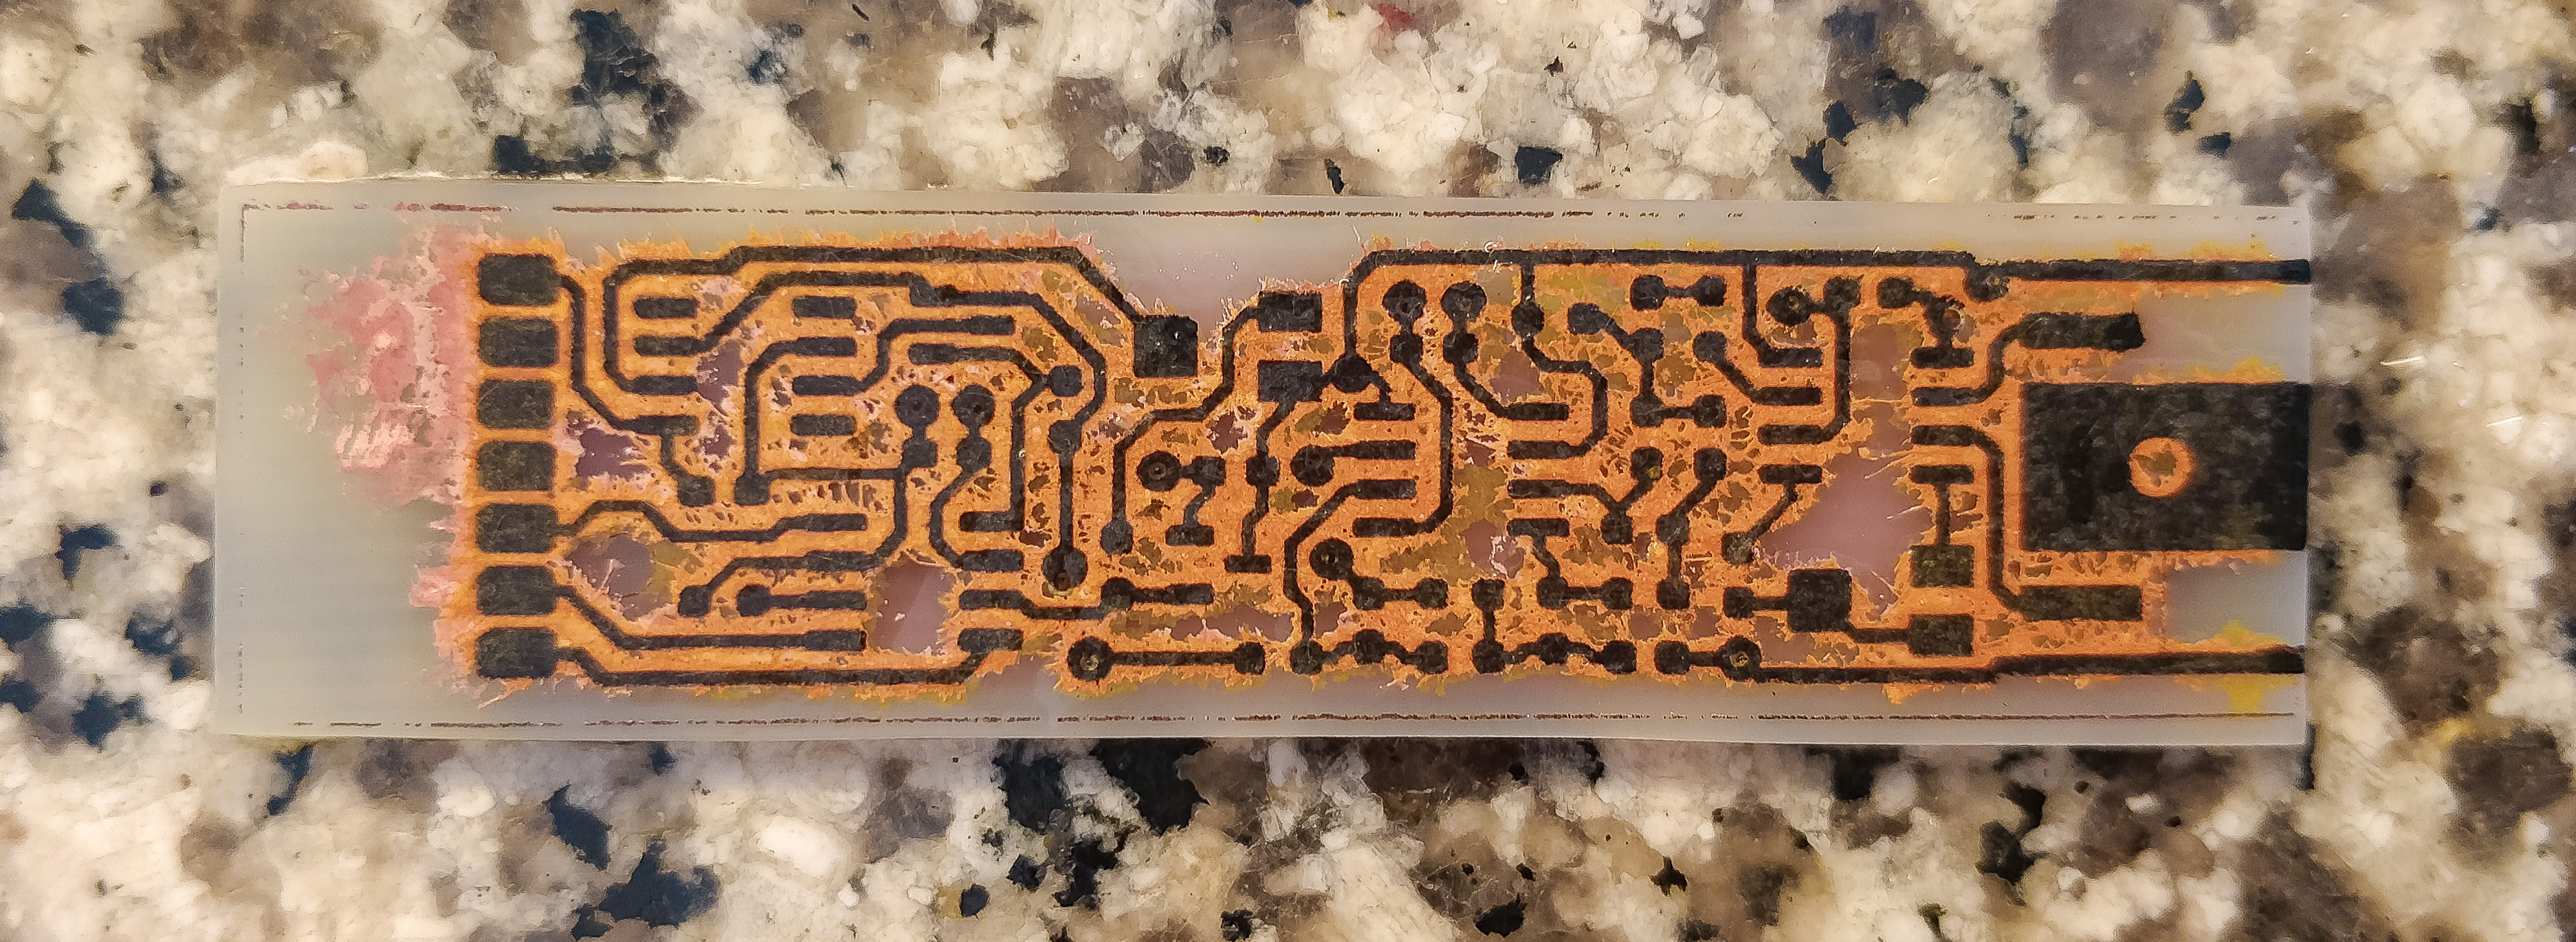
\includegraphics[width=\linewidth]{media/album/PSX_20220228_015716.jpg}
            \caption{}
            \label{fig:PhotoPCBPrepare3}
        \end{minipage}
        \\
        \vspace*{.01\linewidth}
        \begin{minipage}[H]{.95\linewidth}
            \centering
            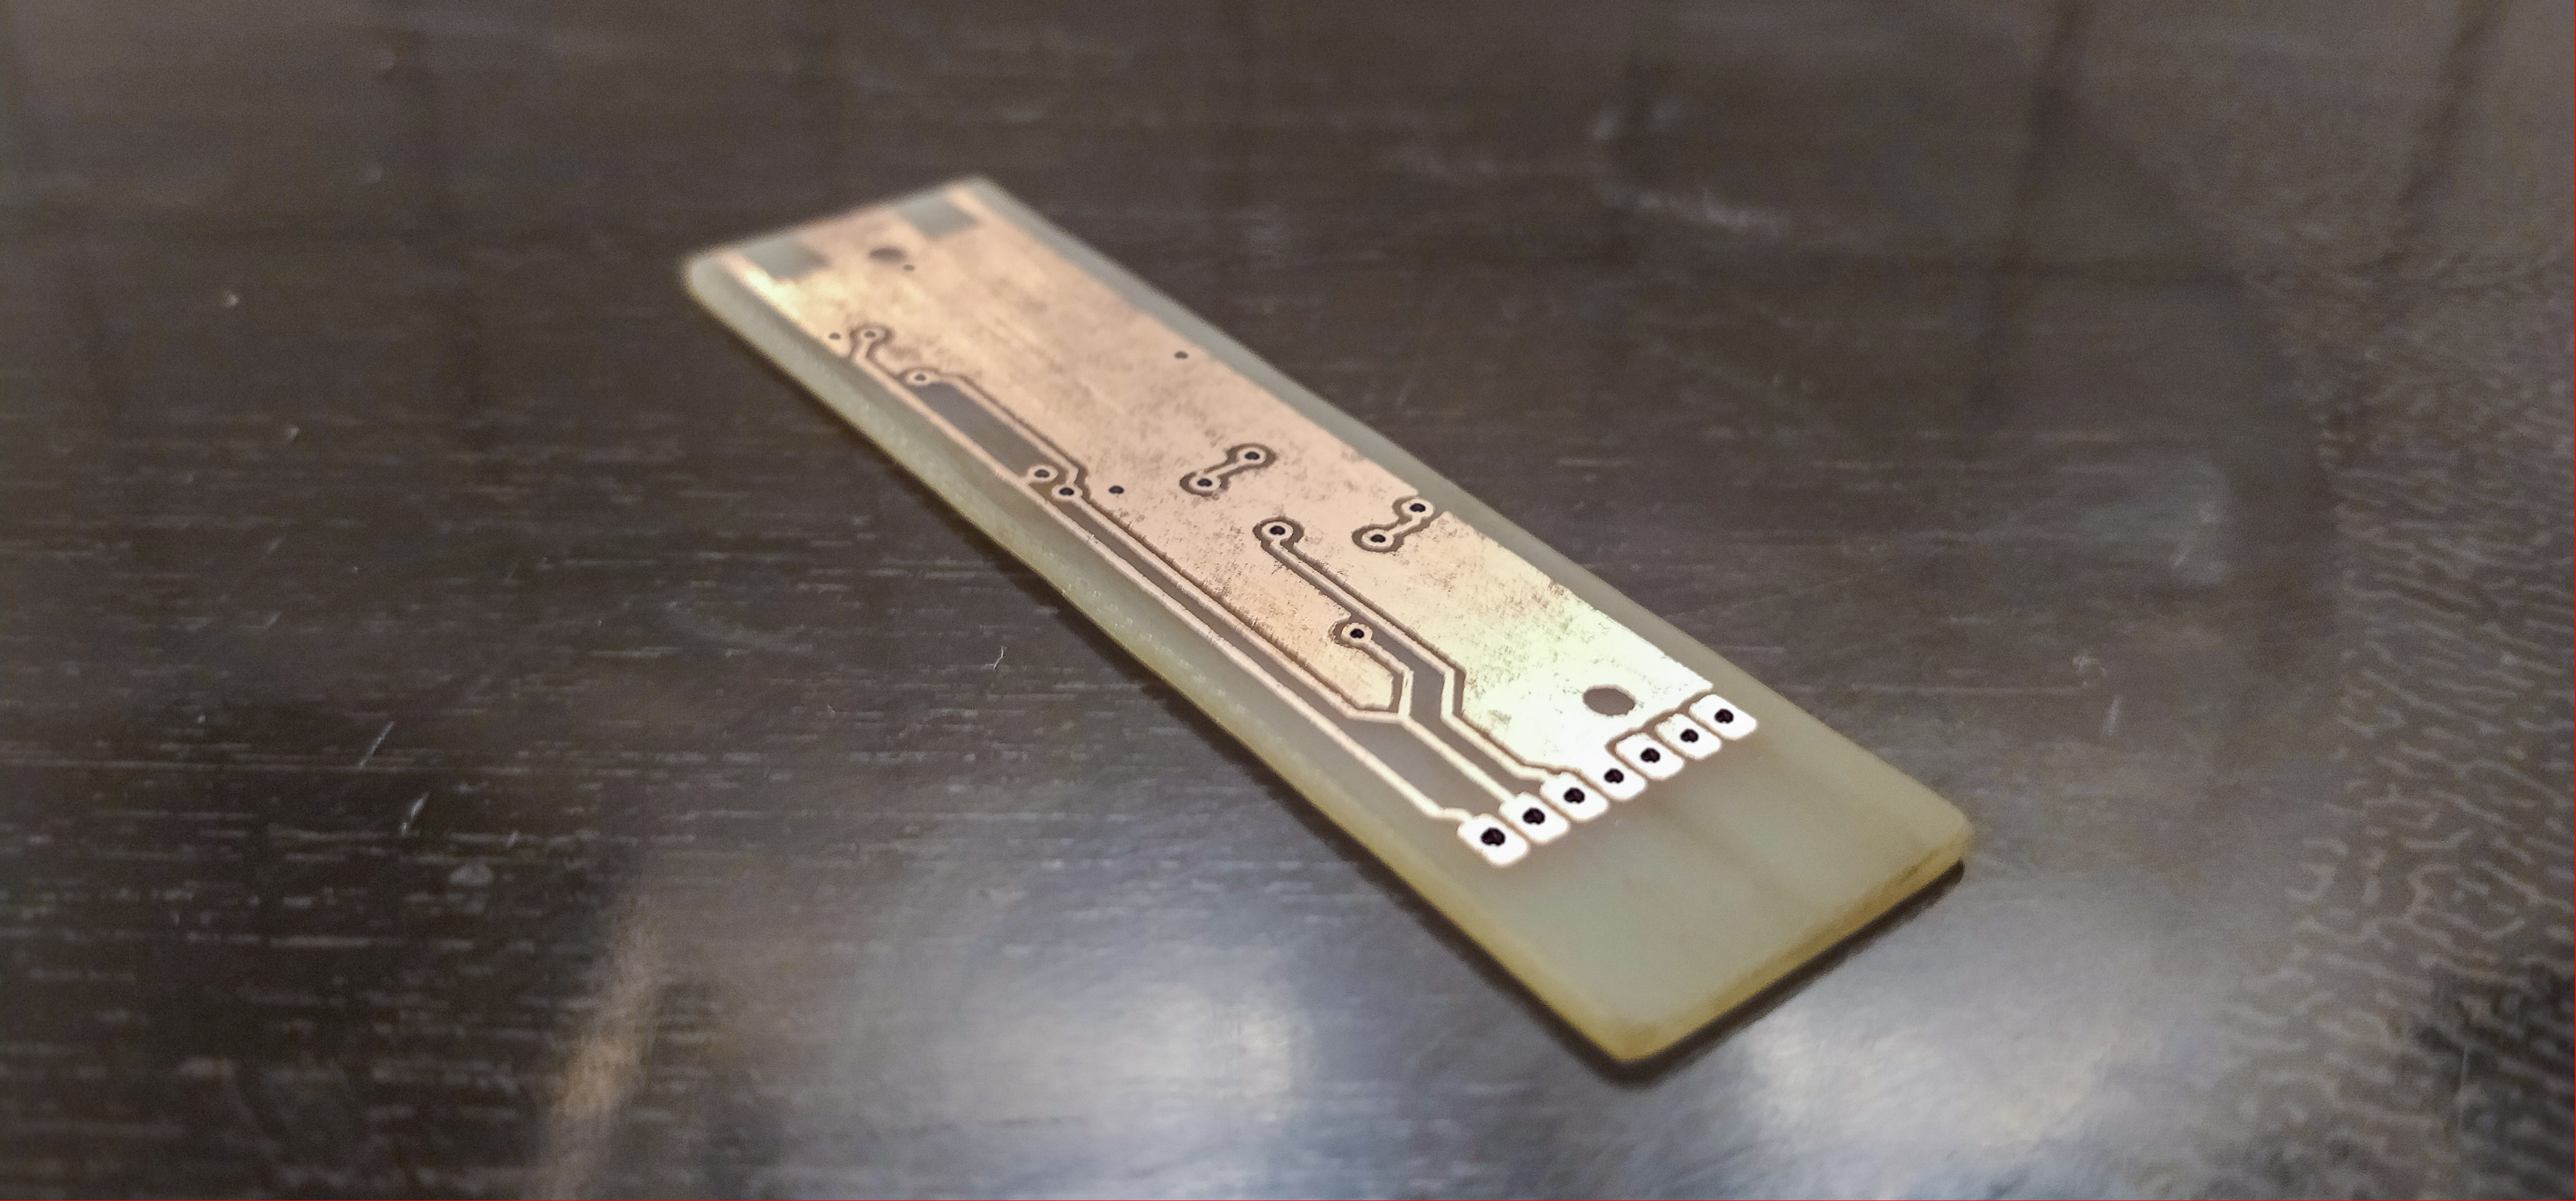
\includegraphics[width=\linewidth]{media/album/PSX_20220301_054445.jpg}
            \caption{}
            \label{fig:PhotoPCBPrepareDone}
        \end{minipage}
    \end{figure}

    The next step is soldering\footnote{Figures \ref{fig:PhotoPCBProgress1}, \ref{fig:PhotoPCBProgress2}, \ref{fig:PhotoPCBProgress3}, \ref{fig:PhotoCableProgress4}, \ref{fig:PhotoCableProgress5}} the circuit, and here fine motor skills come into play.
    % TRANSLATOR NOTE: "antiossidante" (antioxidant) translated as "flux", which is what is meant in soldering.
    The only advice I can give is to pay attention to the flux you use, because some types conduct electricity and, if not completely removed\footnote{With SMD components it cannot be removed from underneath the soldered part} after soldering, can cause malfunctions.
    \begin{figure}[H]
        \centering
        \begin{minipage}[H]{.45\linewidth}
            \centering
            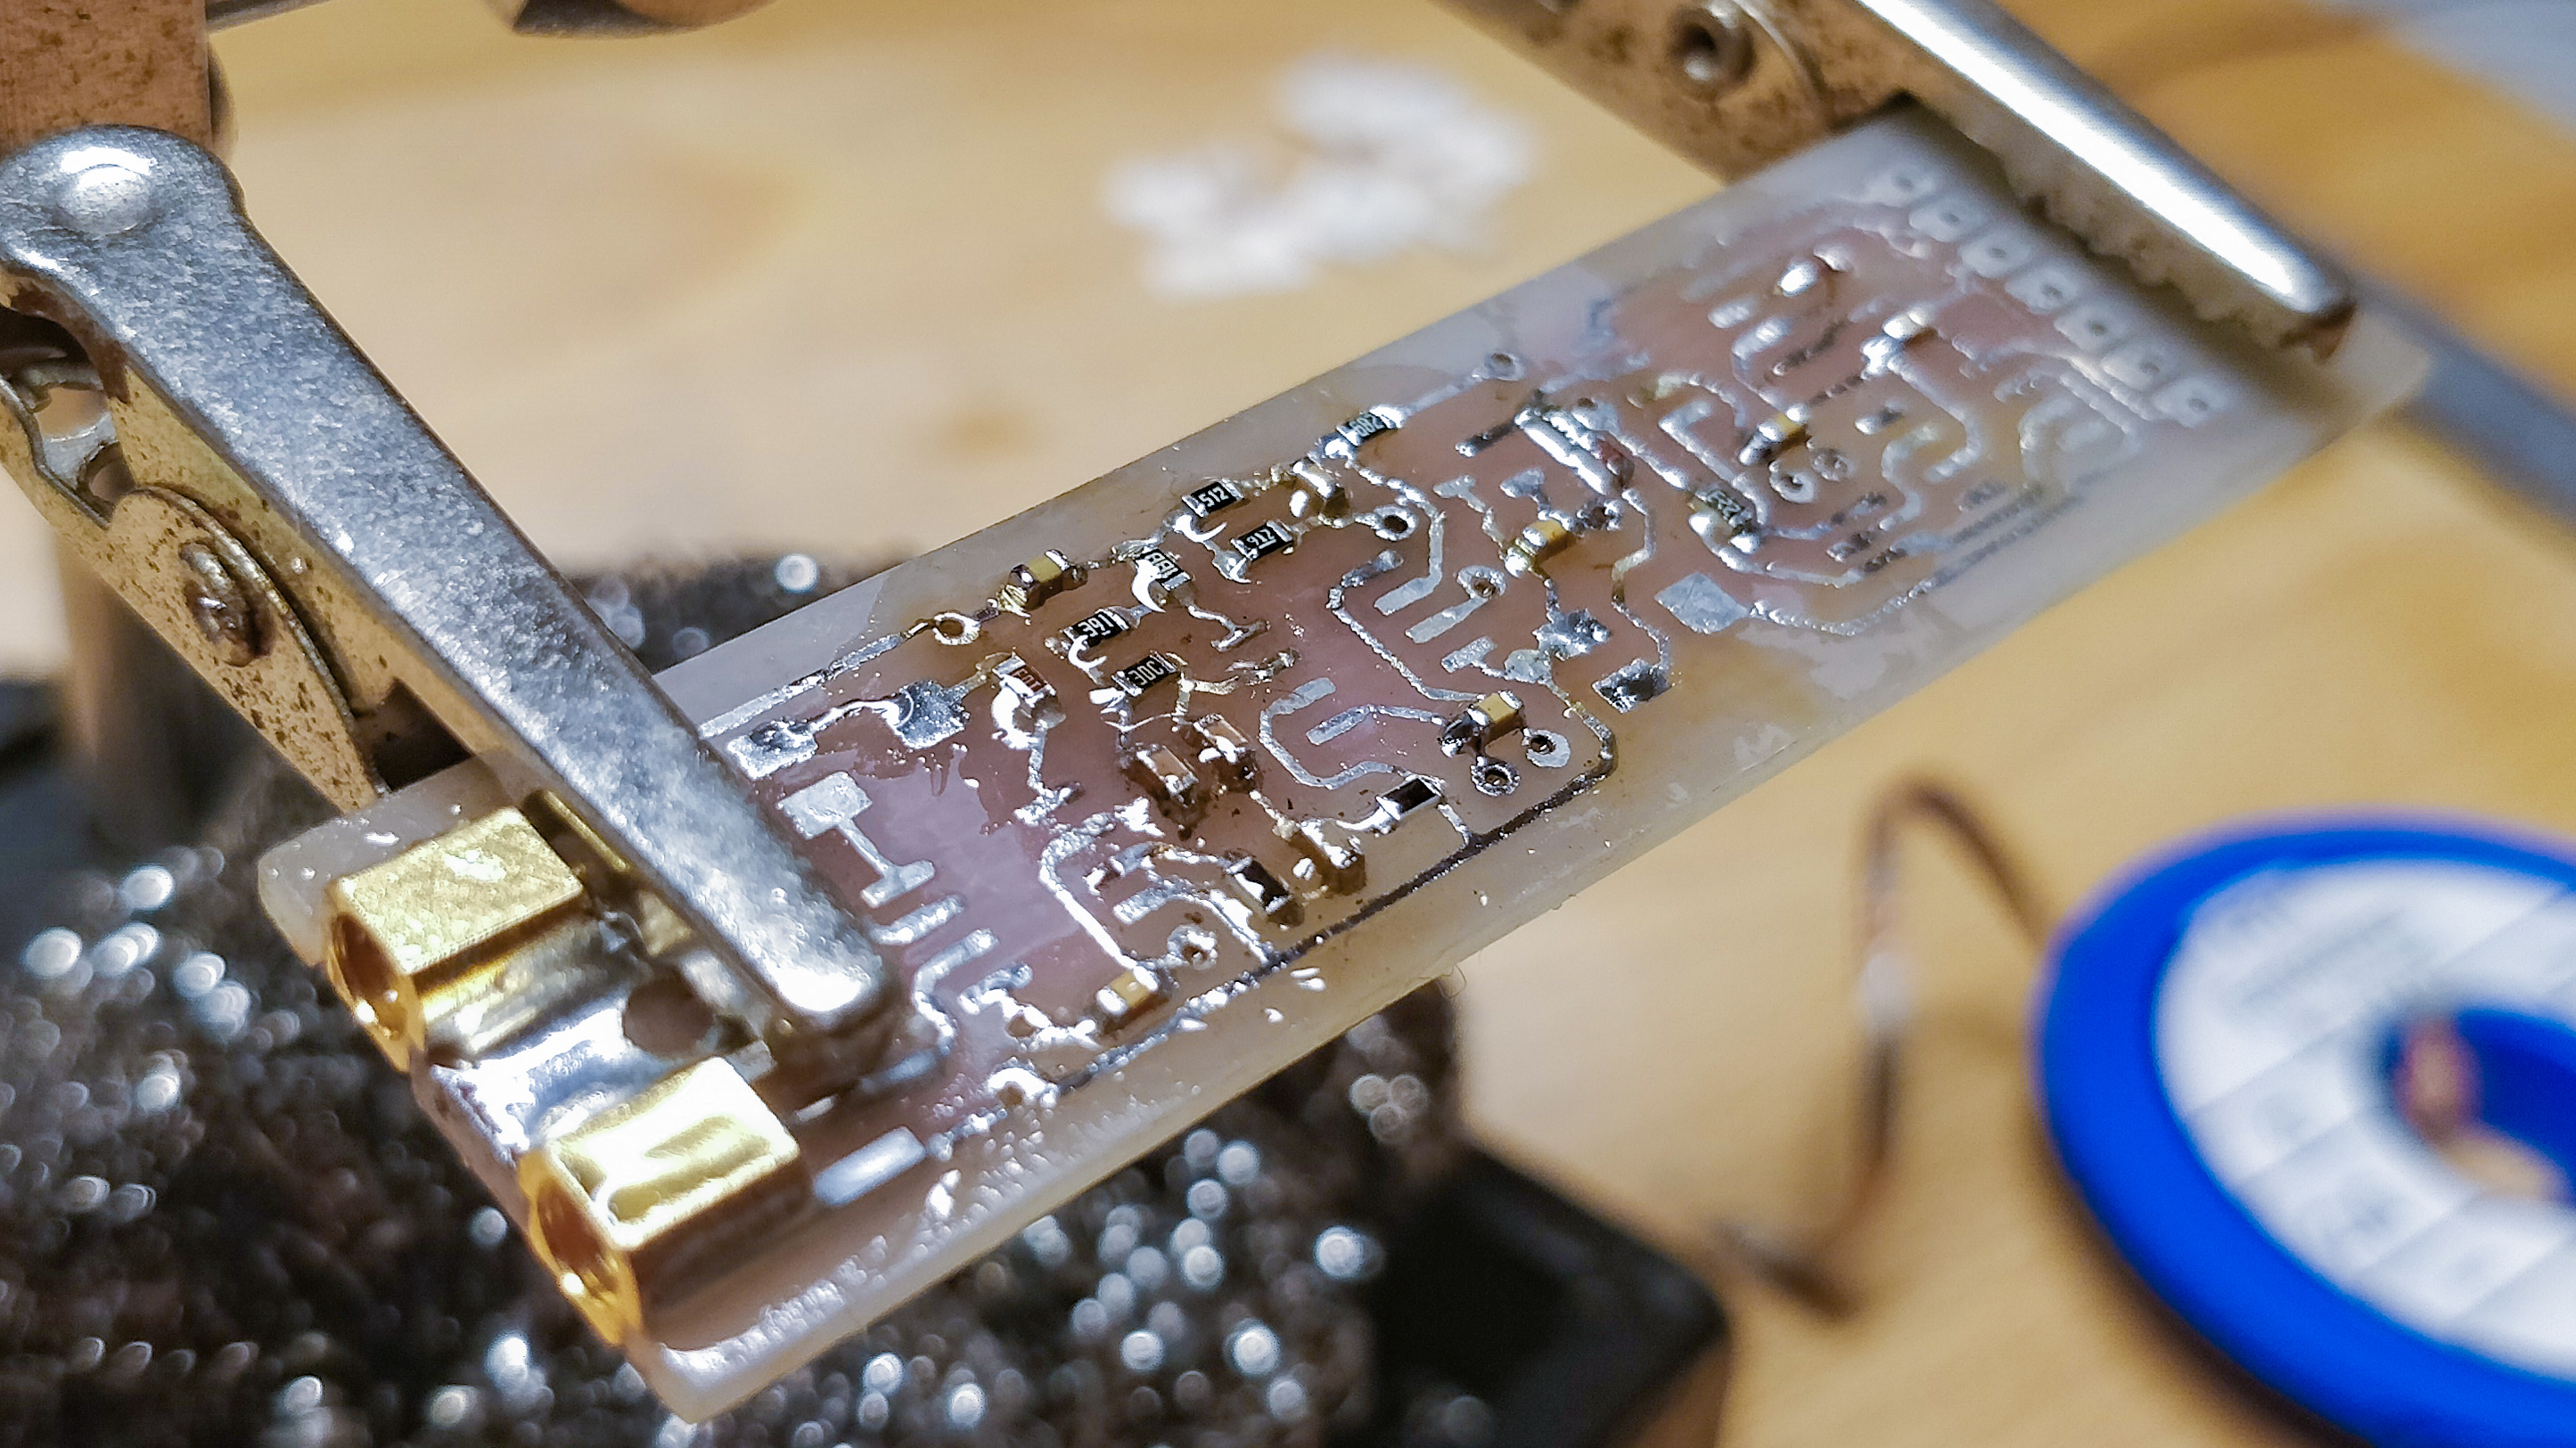
\includegraphics[width=\linewidth]{media/album/PSX_20220228_161847.jpg}
            \caption{}
            \label{fig:PhotoPCBProgress1}
        \end{minipage}
        \hspace{.04\linewidth}
        \begin{minipage}[H]{.45\linewidth}
            \centering
            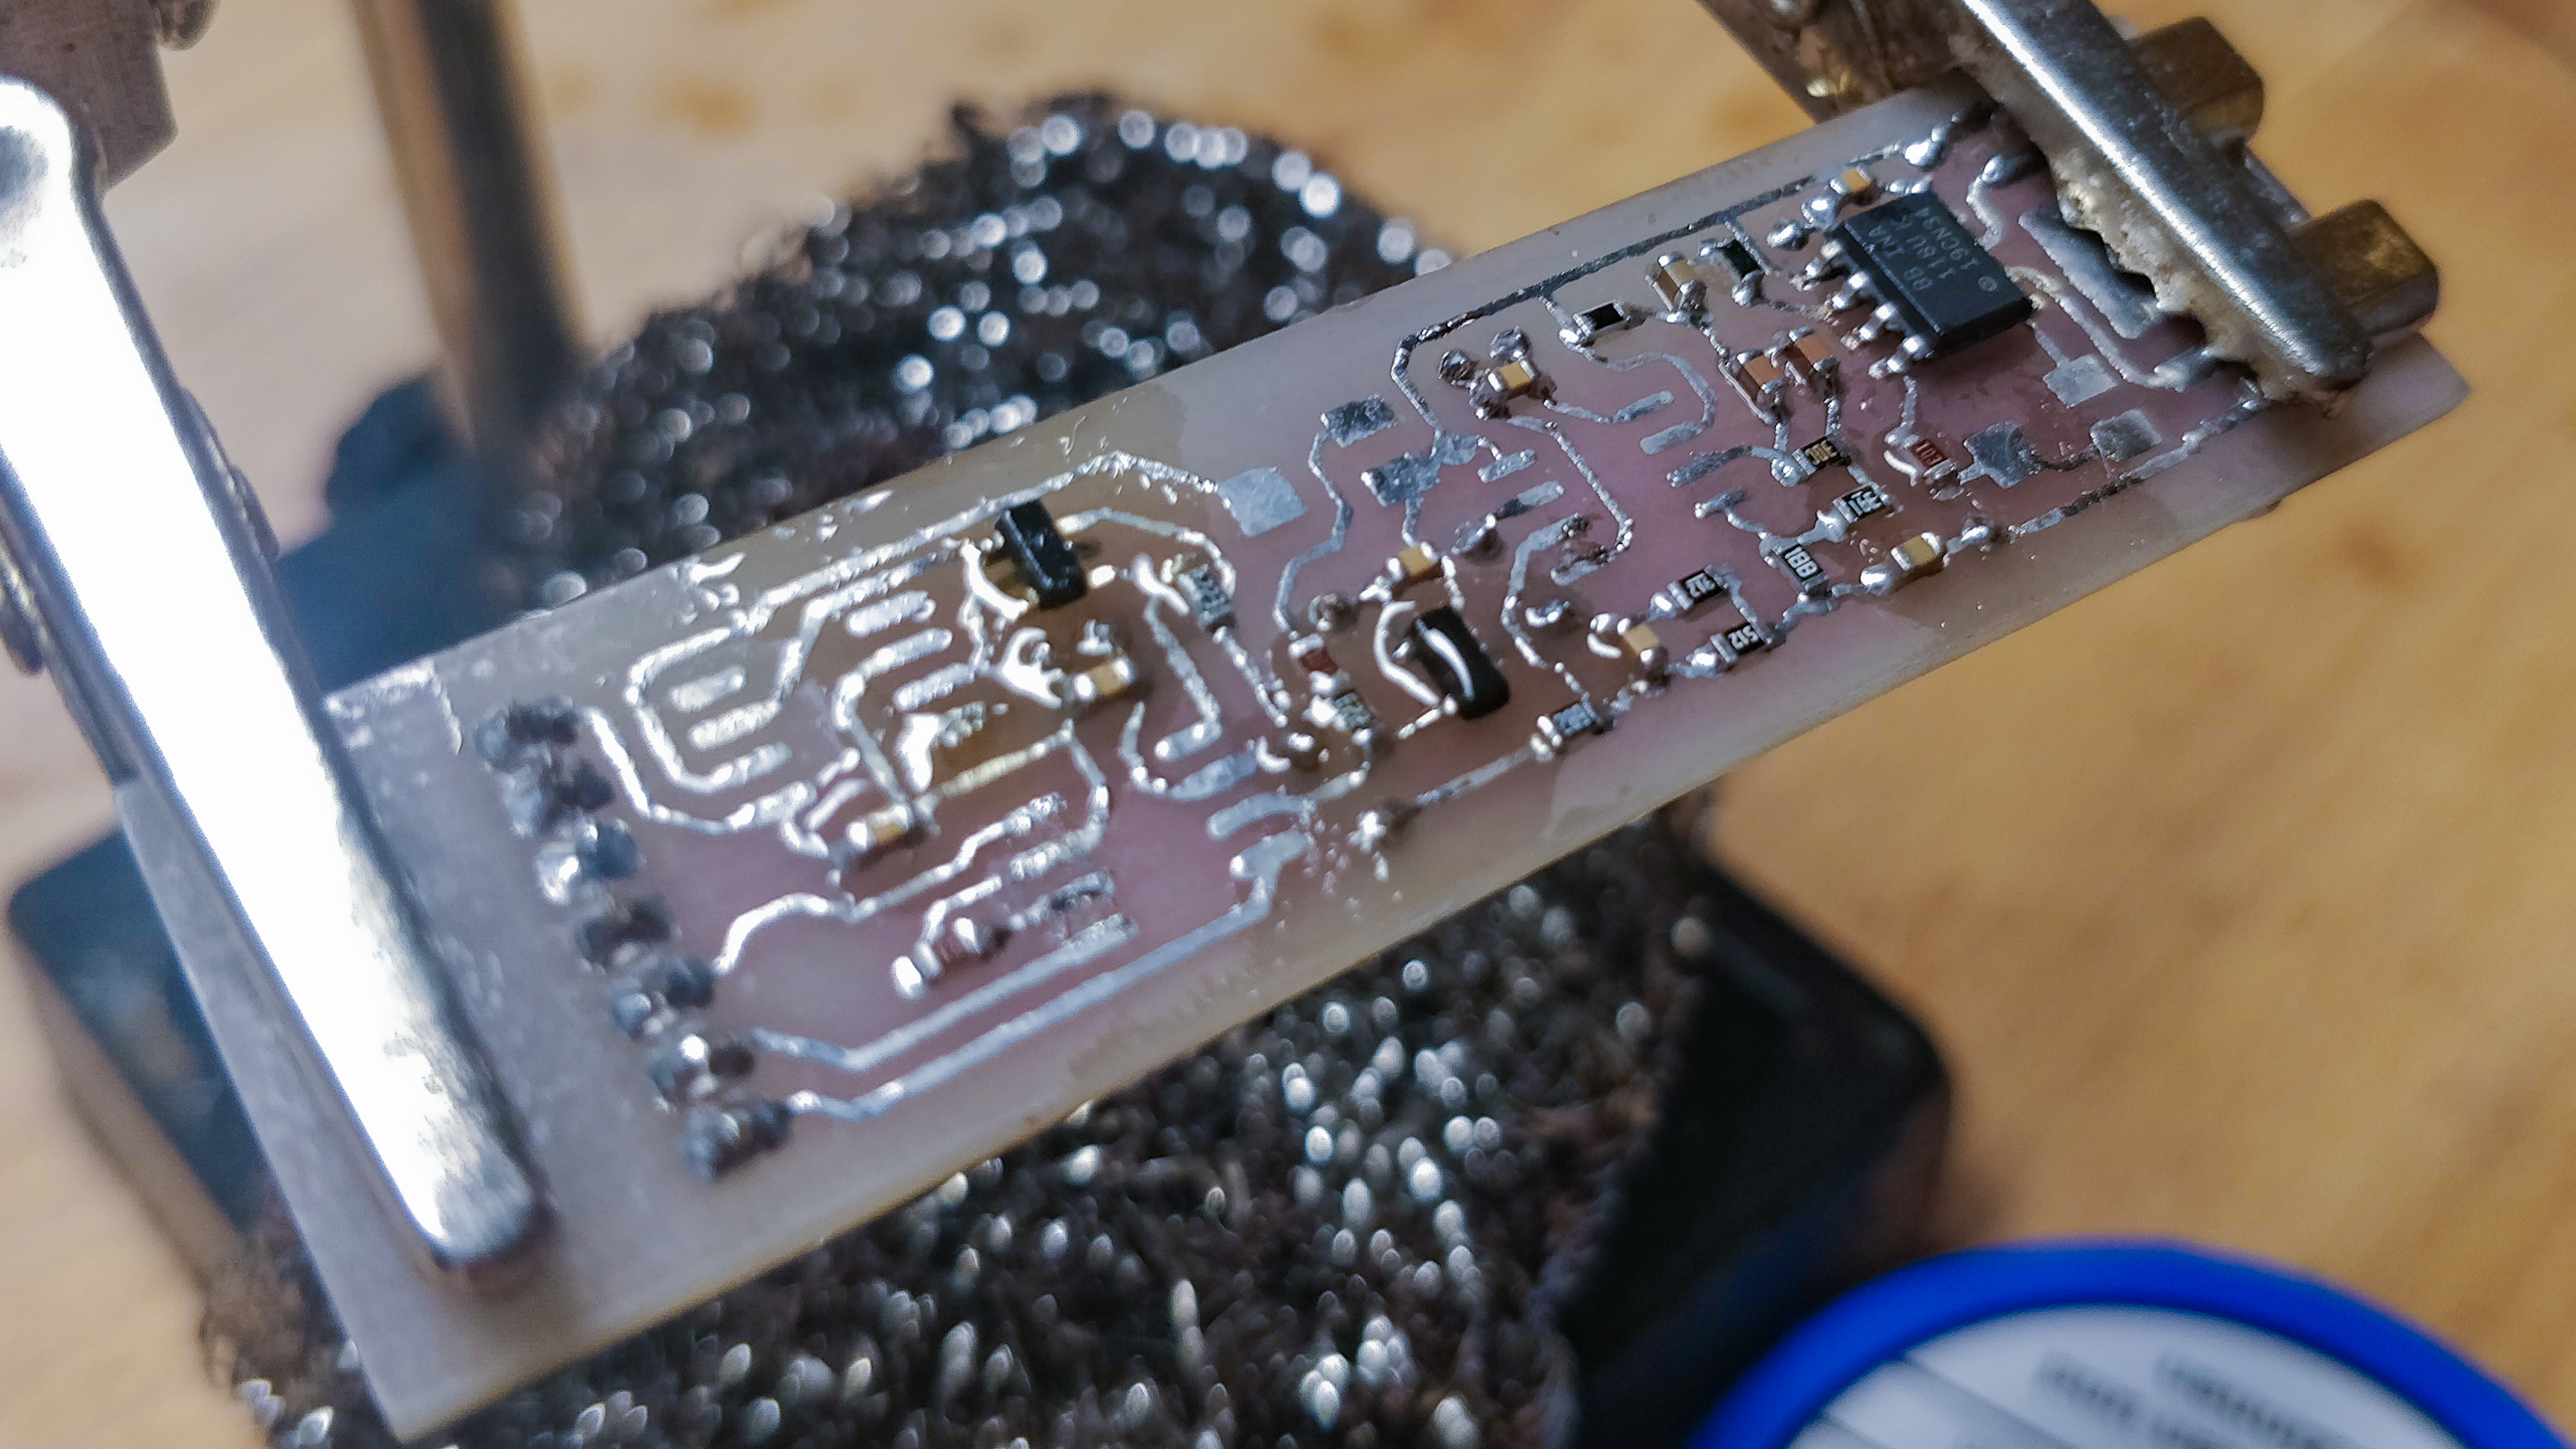
\includegraphics[width=\linewidth]{media/album/PSX_20220228_162014.jpg}
            \caption{}
            \label{fig:PhotoPCBProgress2}
        \end{minipage}
        \\
        \vspace*{.01\linewidth}
        \begin{minipage}[H]{.95\linewidth}
            \centering
            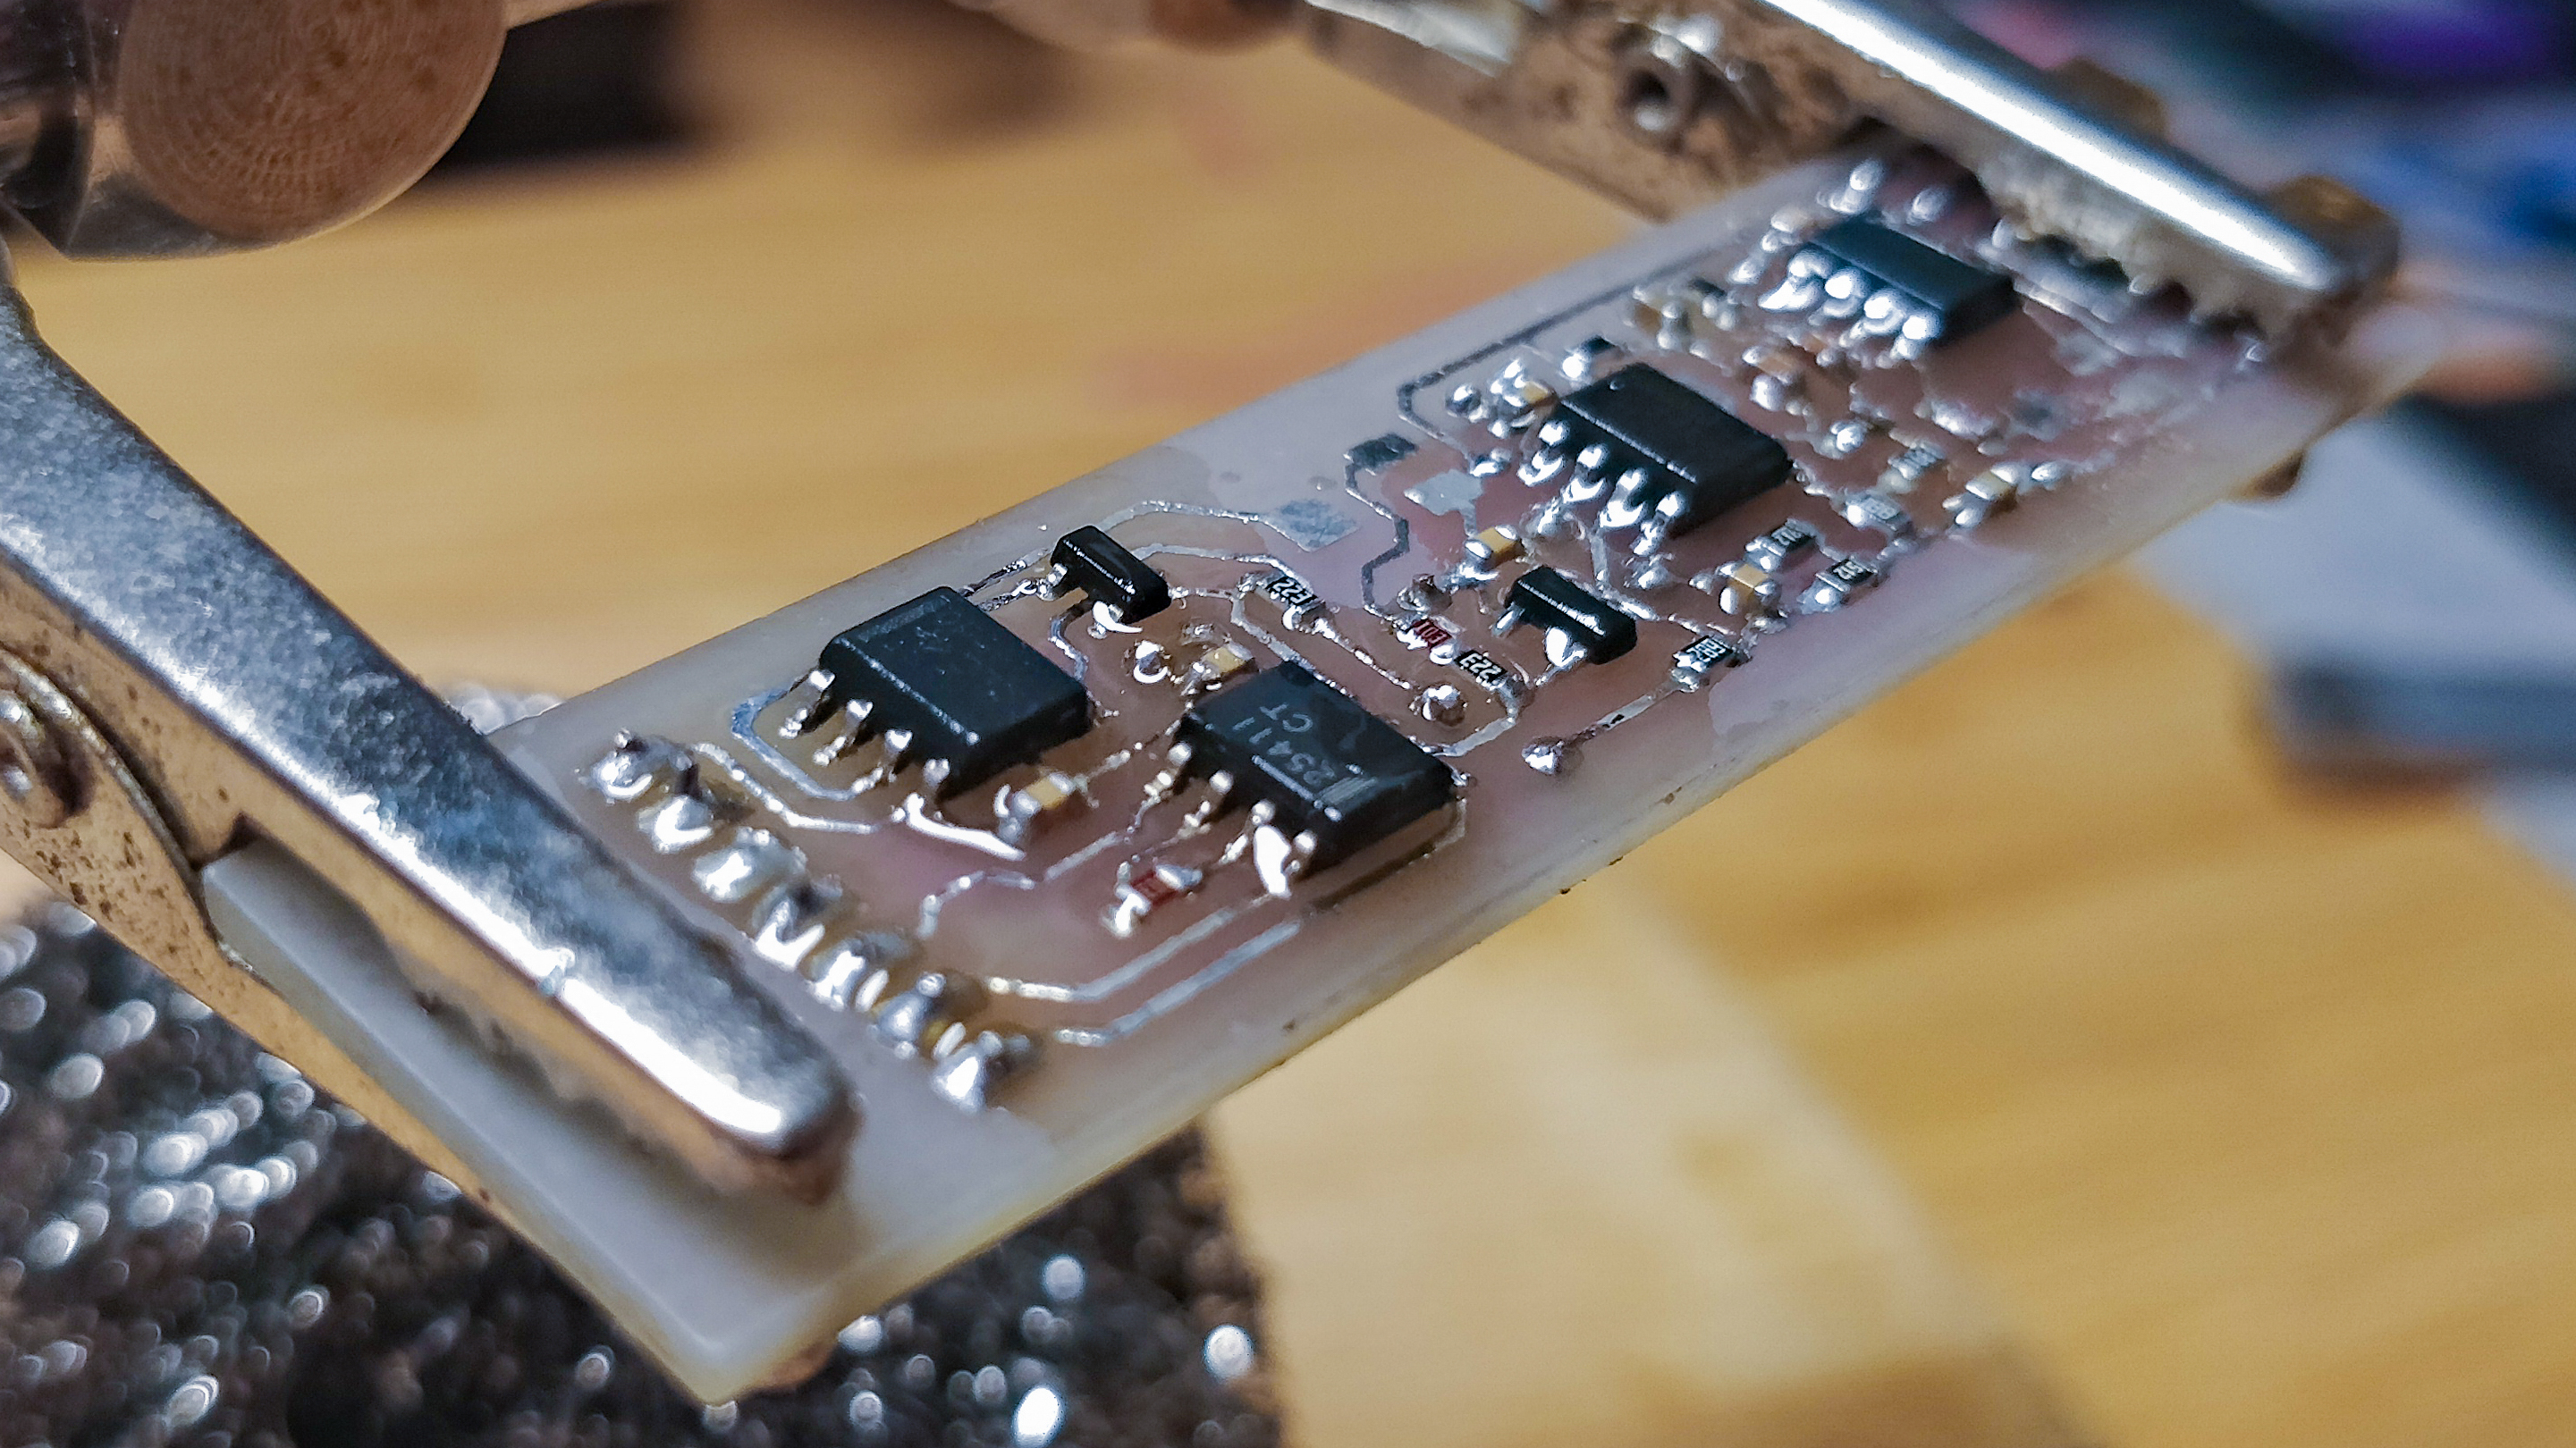
\includegraphics[width=\linewidth]{media/album/PSX_20220301_044735.jpg}
            \caption{}
            \label{fig:PhotoPCBProgress3}
        \end{minipage}
        \\
        \vspace*{.01\linewidth}
        \begin{minipage}[H]{.95\linewidth}
            \centering
            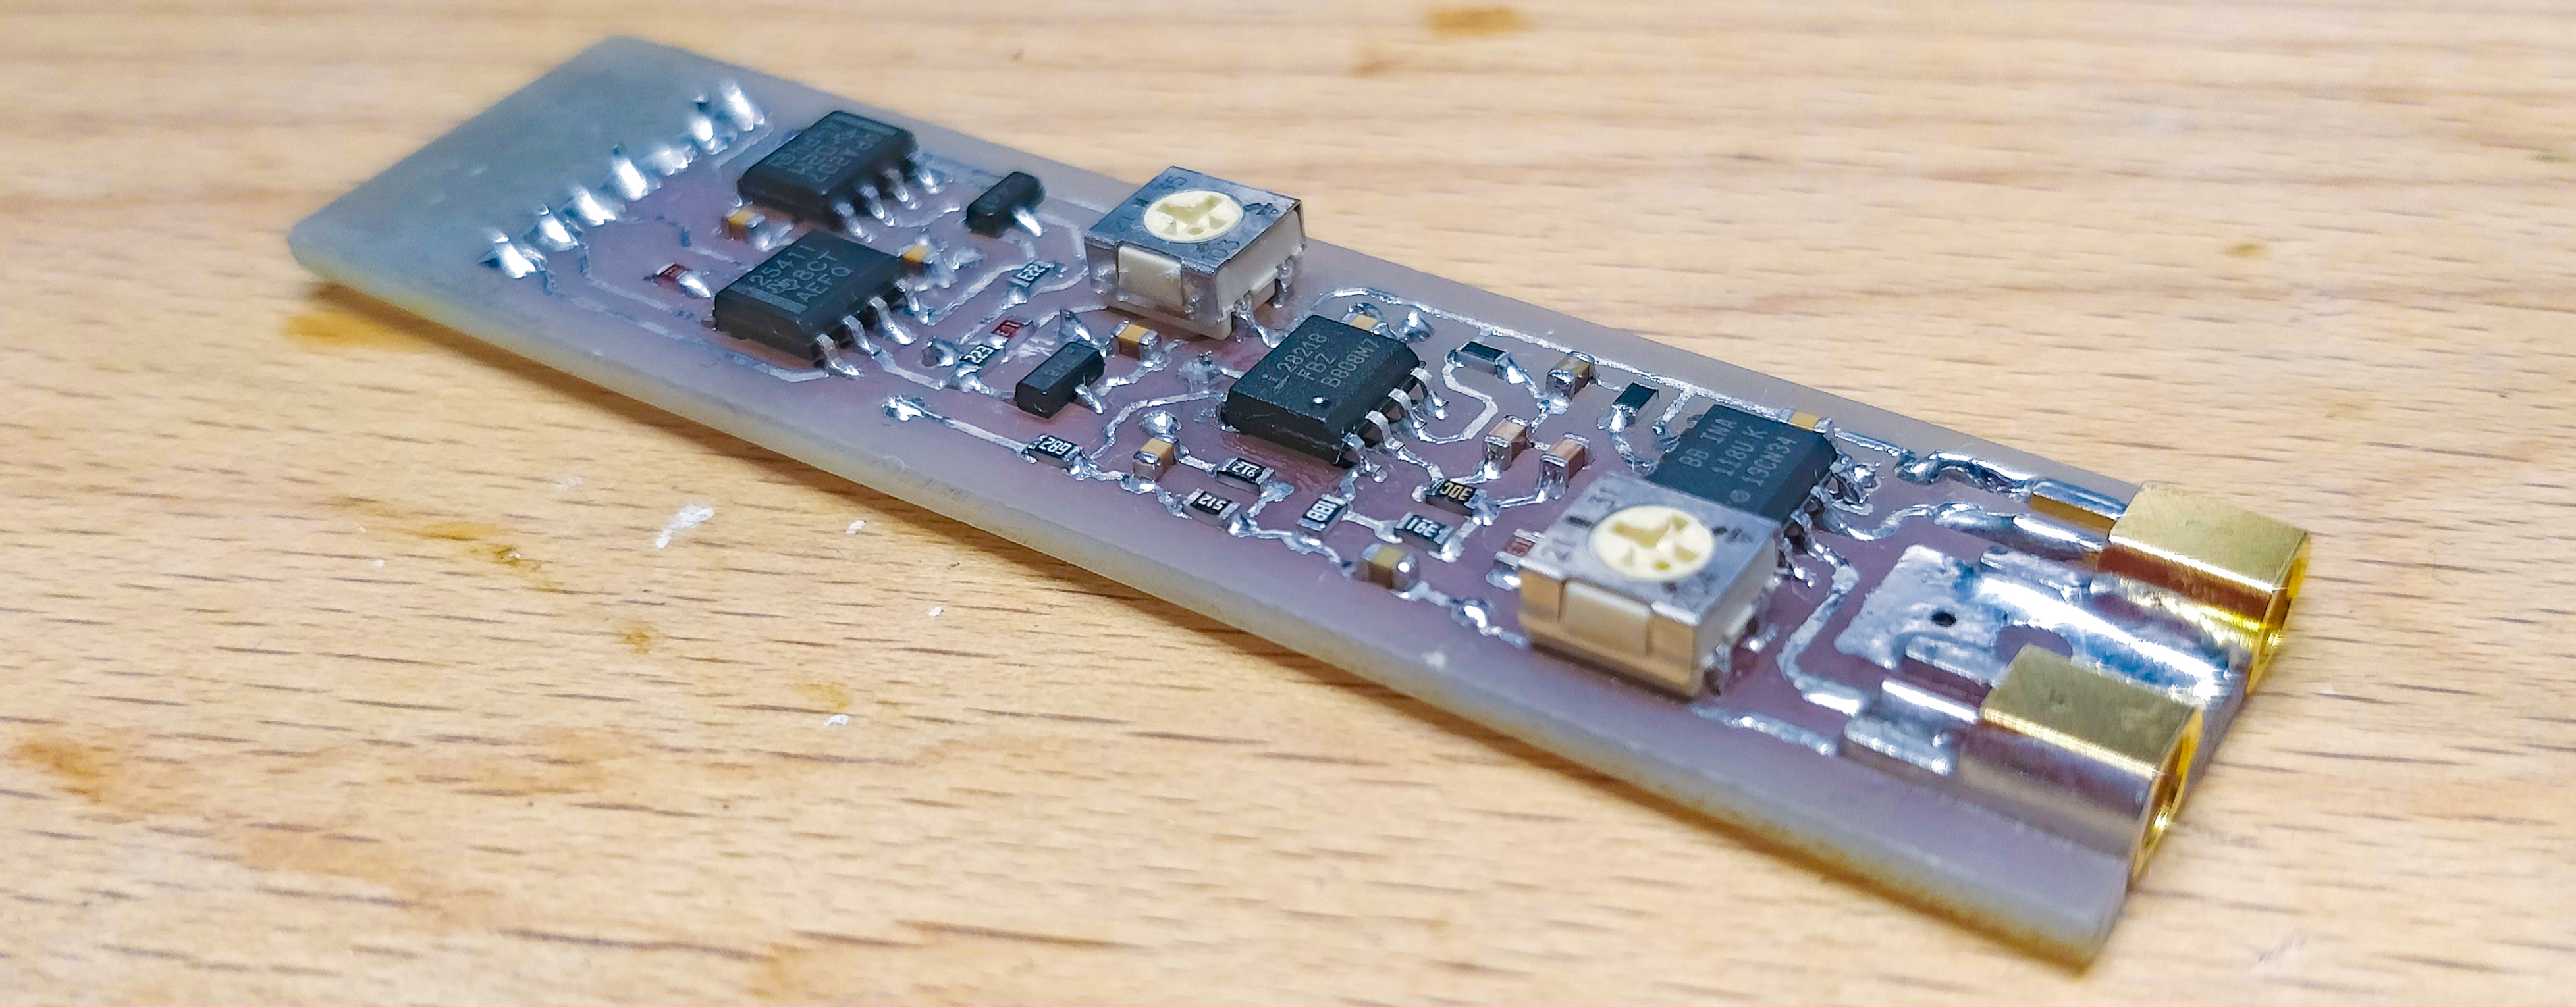
\includegraphics[width=\linewidth]{media/album/PSX_20220228_020356.jpg}
            \caption{}
            \label{fig:PhotoPCBDone}
        \end{minipage}
    \end{figure}

    Because of a small ordering mistake I could not solder connector $J3$, so I soldered wires in its place. With the soldering of the electrode cables\footnote{Figures \ref{fig:PhotoCableProgress1}, \ref{fig:PhotoCableProgress2}, \ref{fig:PhotoCableProgress3}, \ref{fig:PhotoCableProgress4}, \ref{fig:PhotoCableProgress5}, \ref{fig:PhotoCableDone}} the circuit was complete.
    \begin{figure}[H]
        \RaggedRight
        \centering   
        \begin{minipage}[H]{.95\linewidth}
            \centering
            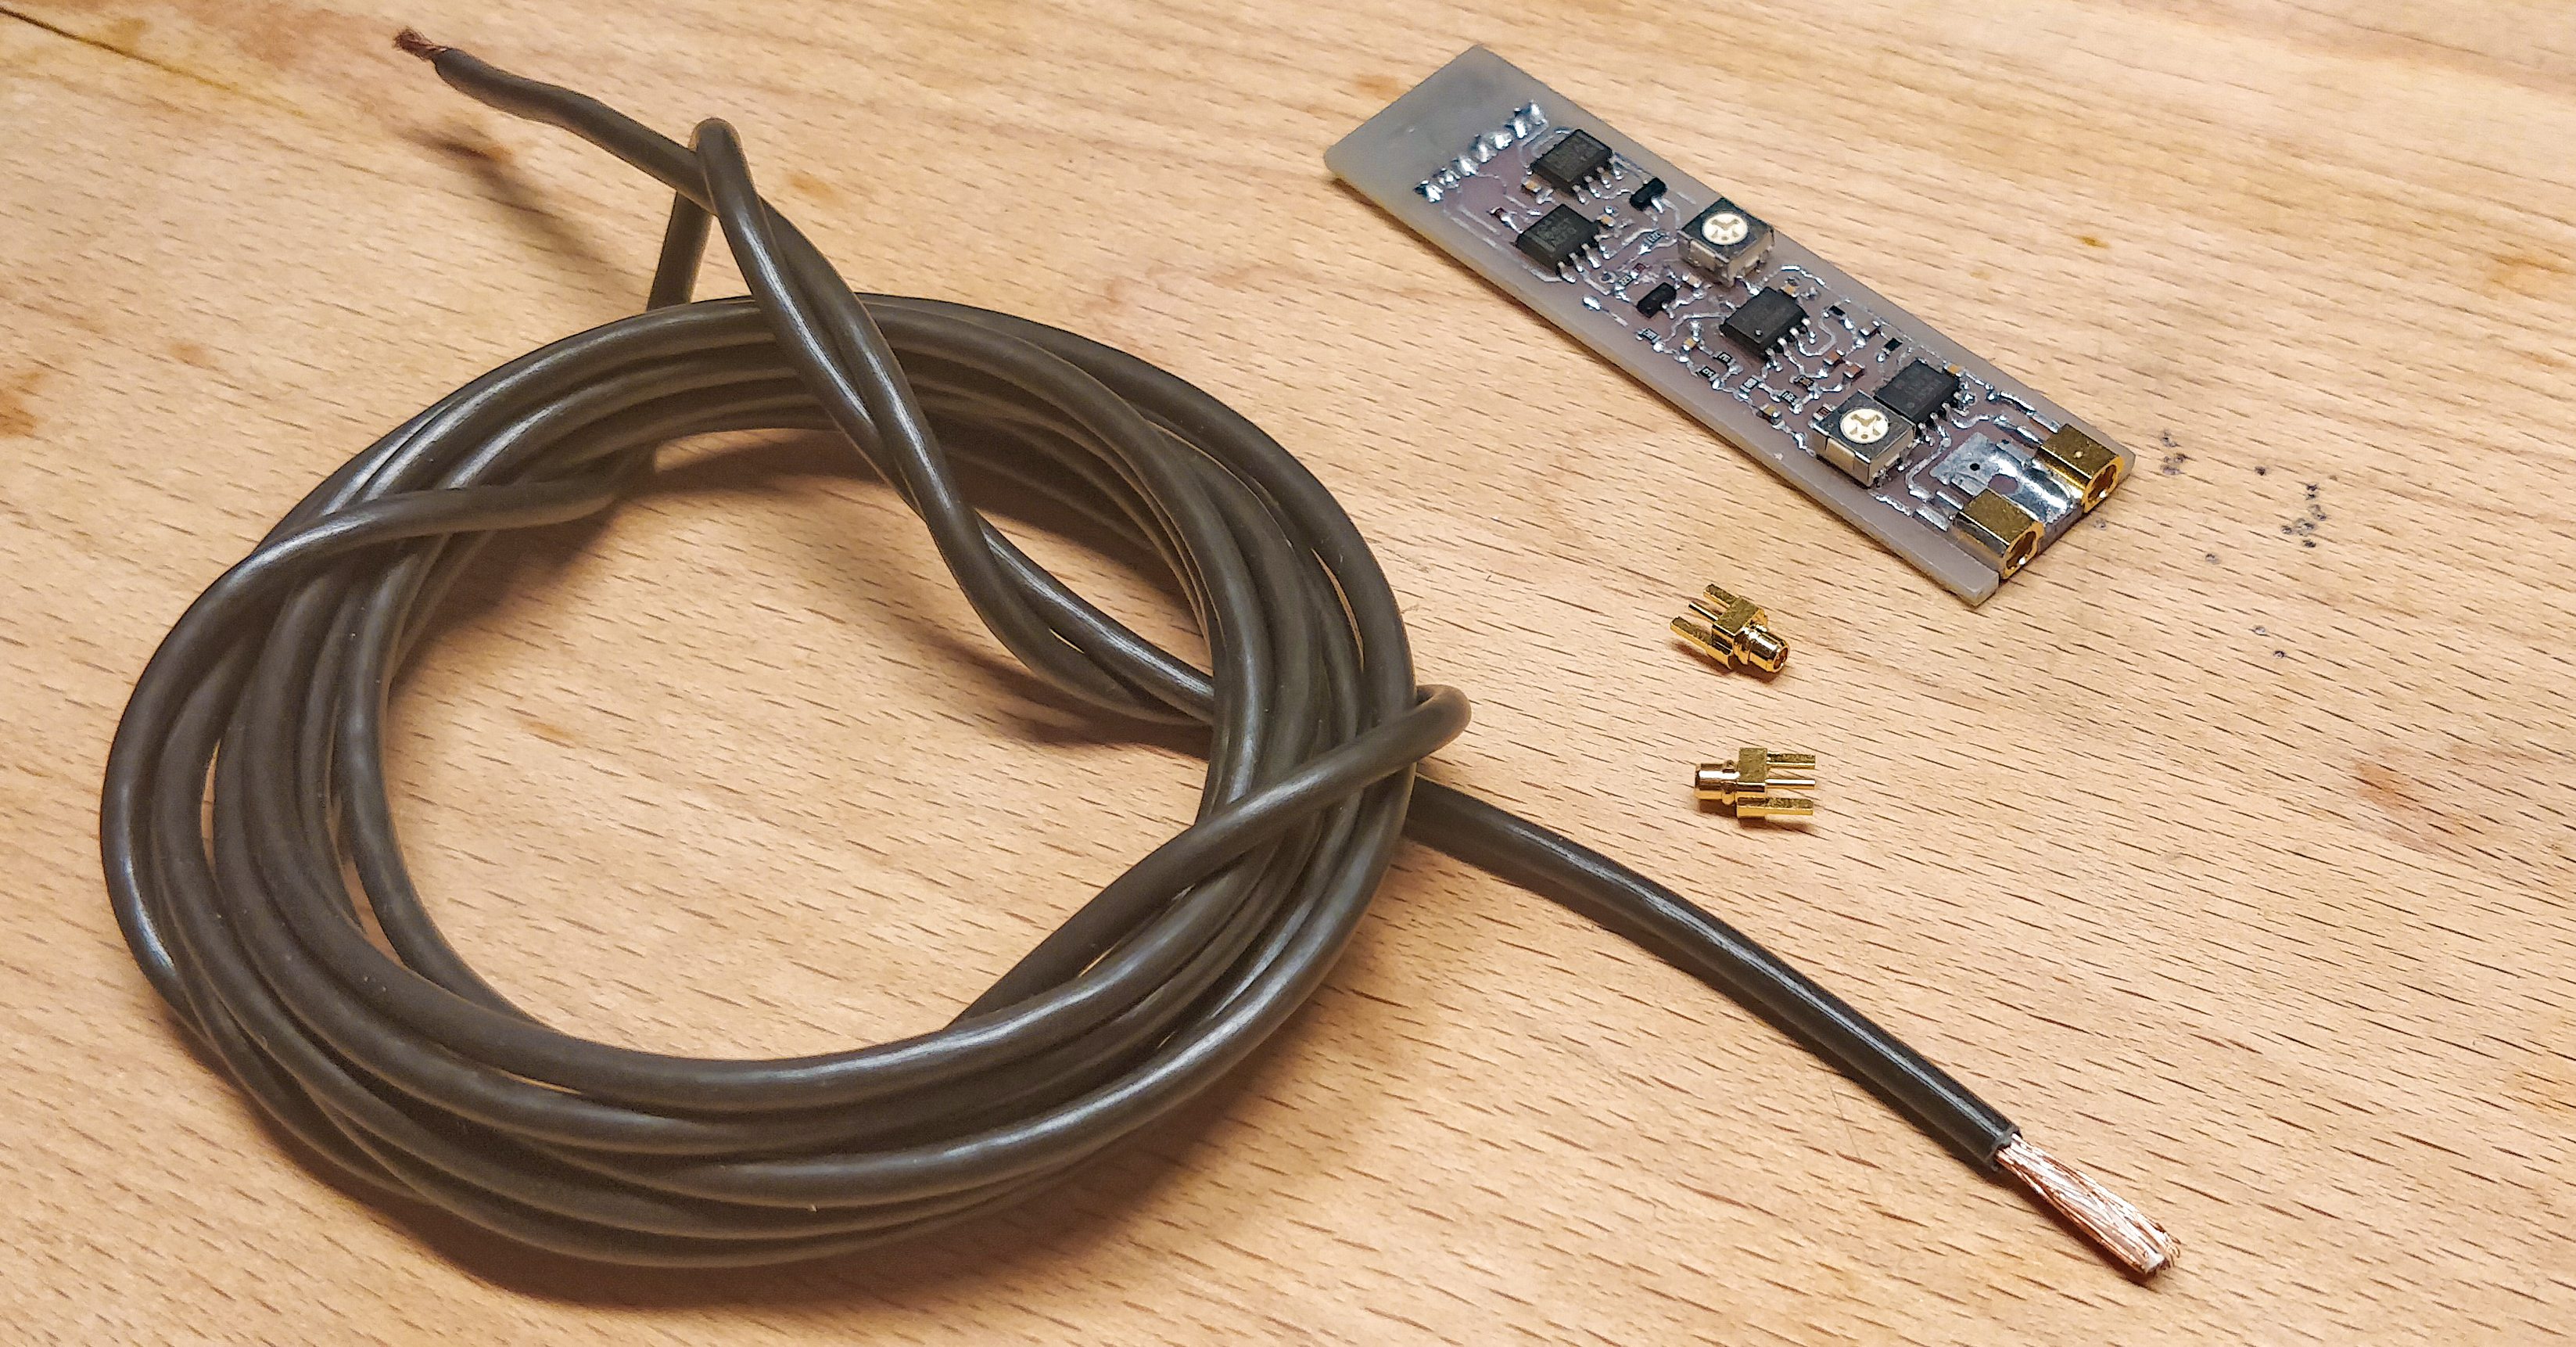
\includegraphics[width=\linewidth]{media/album/PSX_20220228_020856.jpg}
            \caption{}
            \label{fig:PhotoCableProgress1}
        \end{minipage}
        \\
        \vspace*{.01\linewidth}
        \begin{minipage}[H]{.28\linewidth}
            \centering
            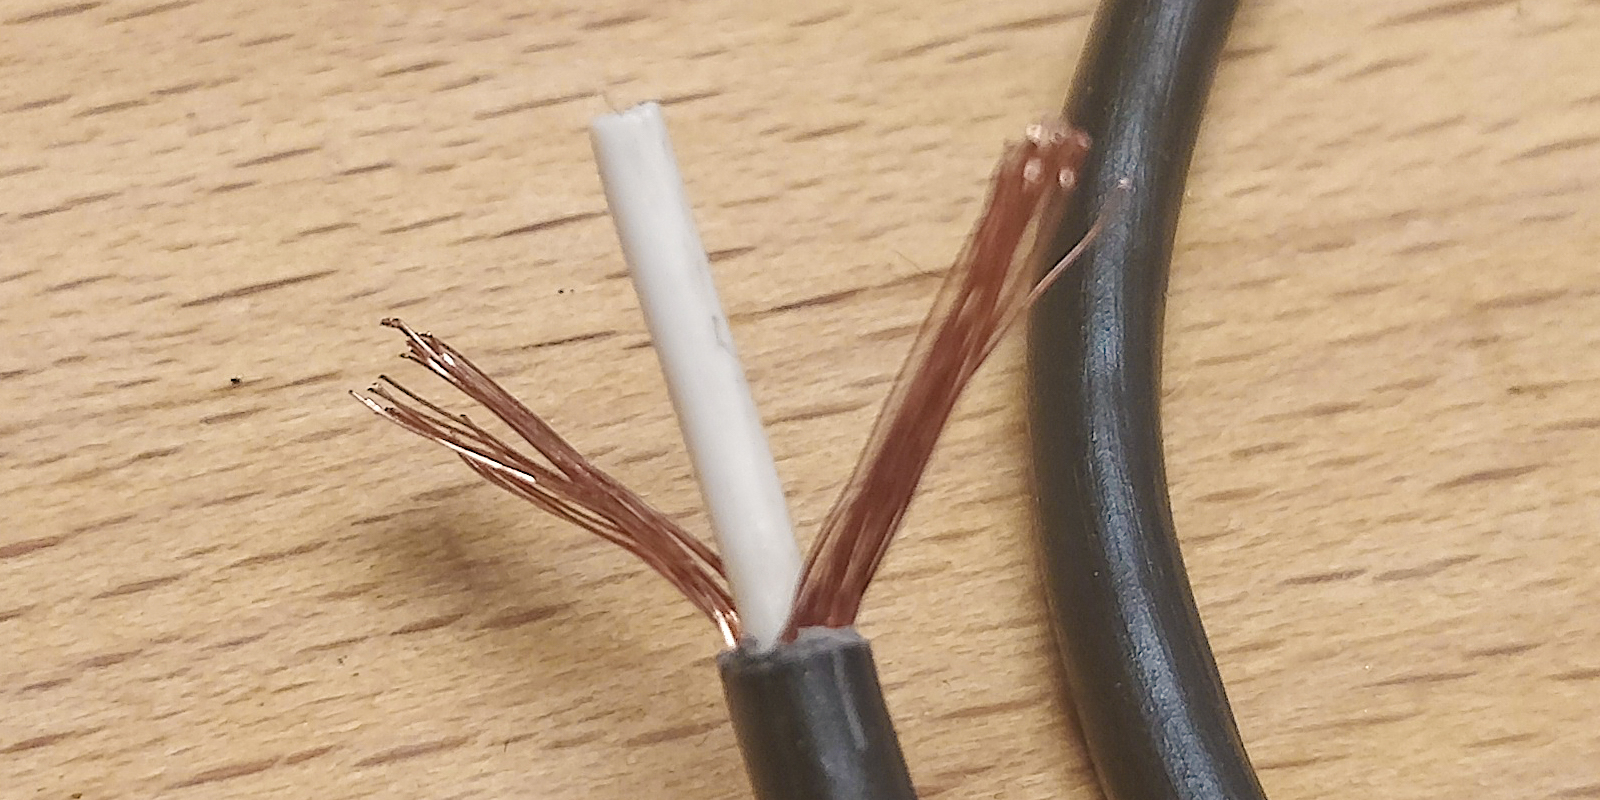
\includegraphics[width=\linewidth]{media/album/PSX_20220228_020741.jpg}
            \caption{}
            \label{fig:PhotoCableProgress2}
        \end{minipage}
        \hspace{.04\linewidth}
        \begin{minipage}[H]{.28\linewidth}
            \centering
            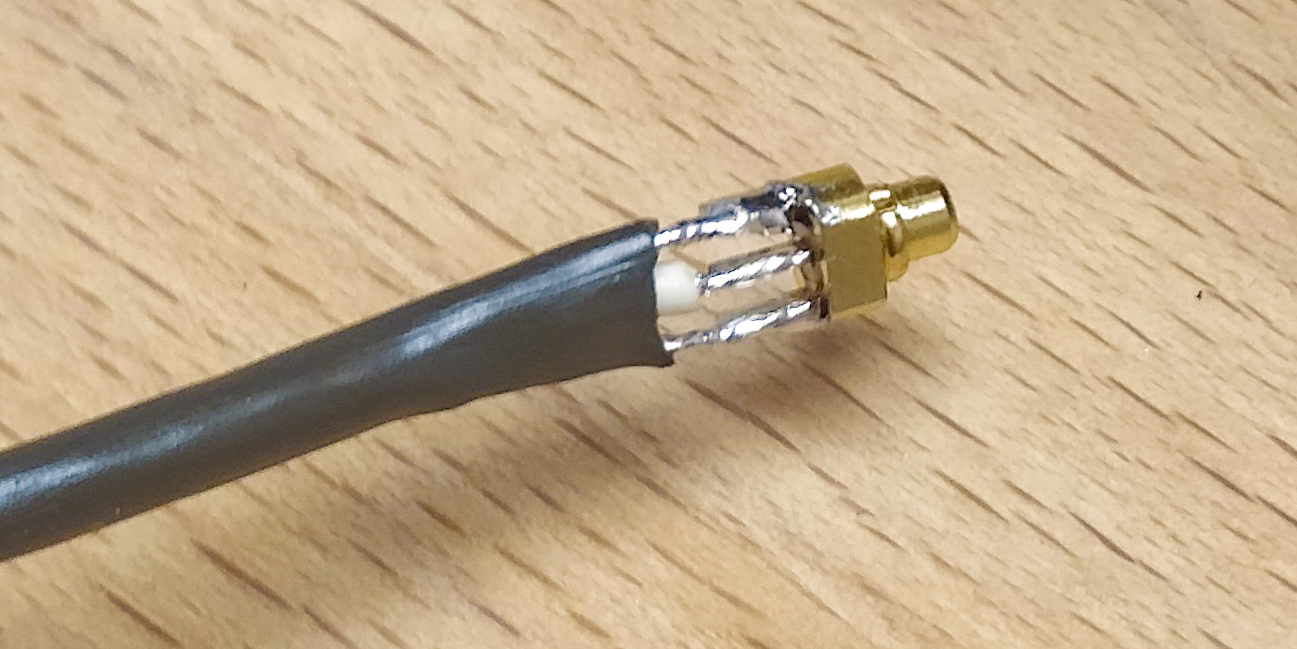
\includegraphics[width=\linewidth]{media/album/PSX_20220228_162153.jpg}
            \caption{}
            \label{fig:PhotoCableProgress3}
        \end{minipage}
        \hspace{.04\linewidth}
        \begin{minipage}[H]{.28\linewidth}
            \centering
            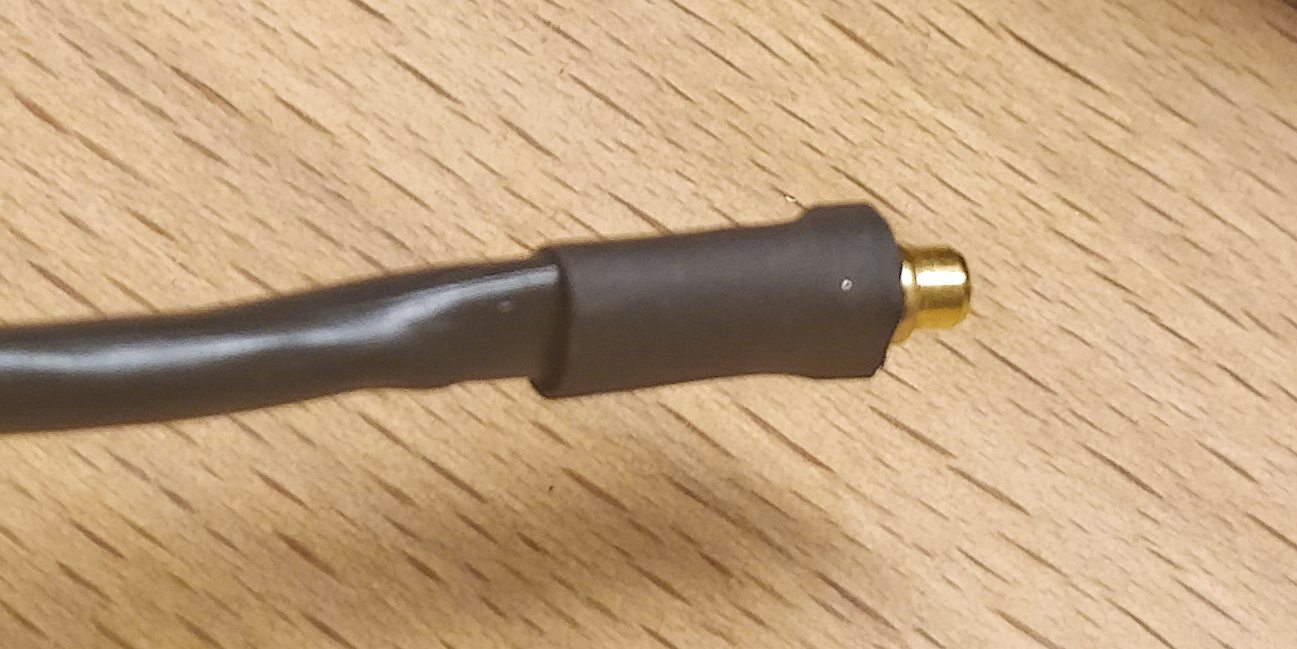
\includegraphics[width=\linewidth]{media/album/PSX_20220228_162233.jpg}
            \caption{}
            \label{fig:PhotoCableProgress4}
        \end{minipage}
        \\
        \vspace*{.01\linewidth}
        \begin{minipage}[H]{.95\linewidth}
            \centering
            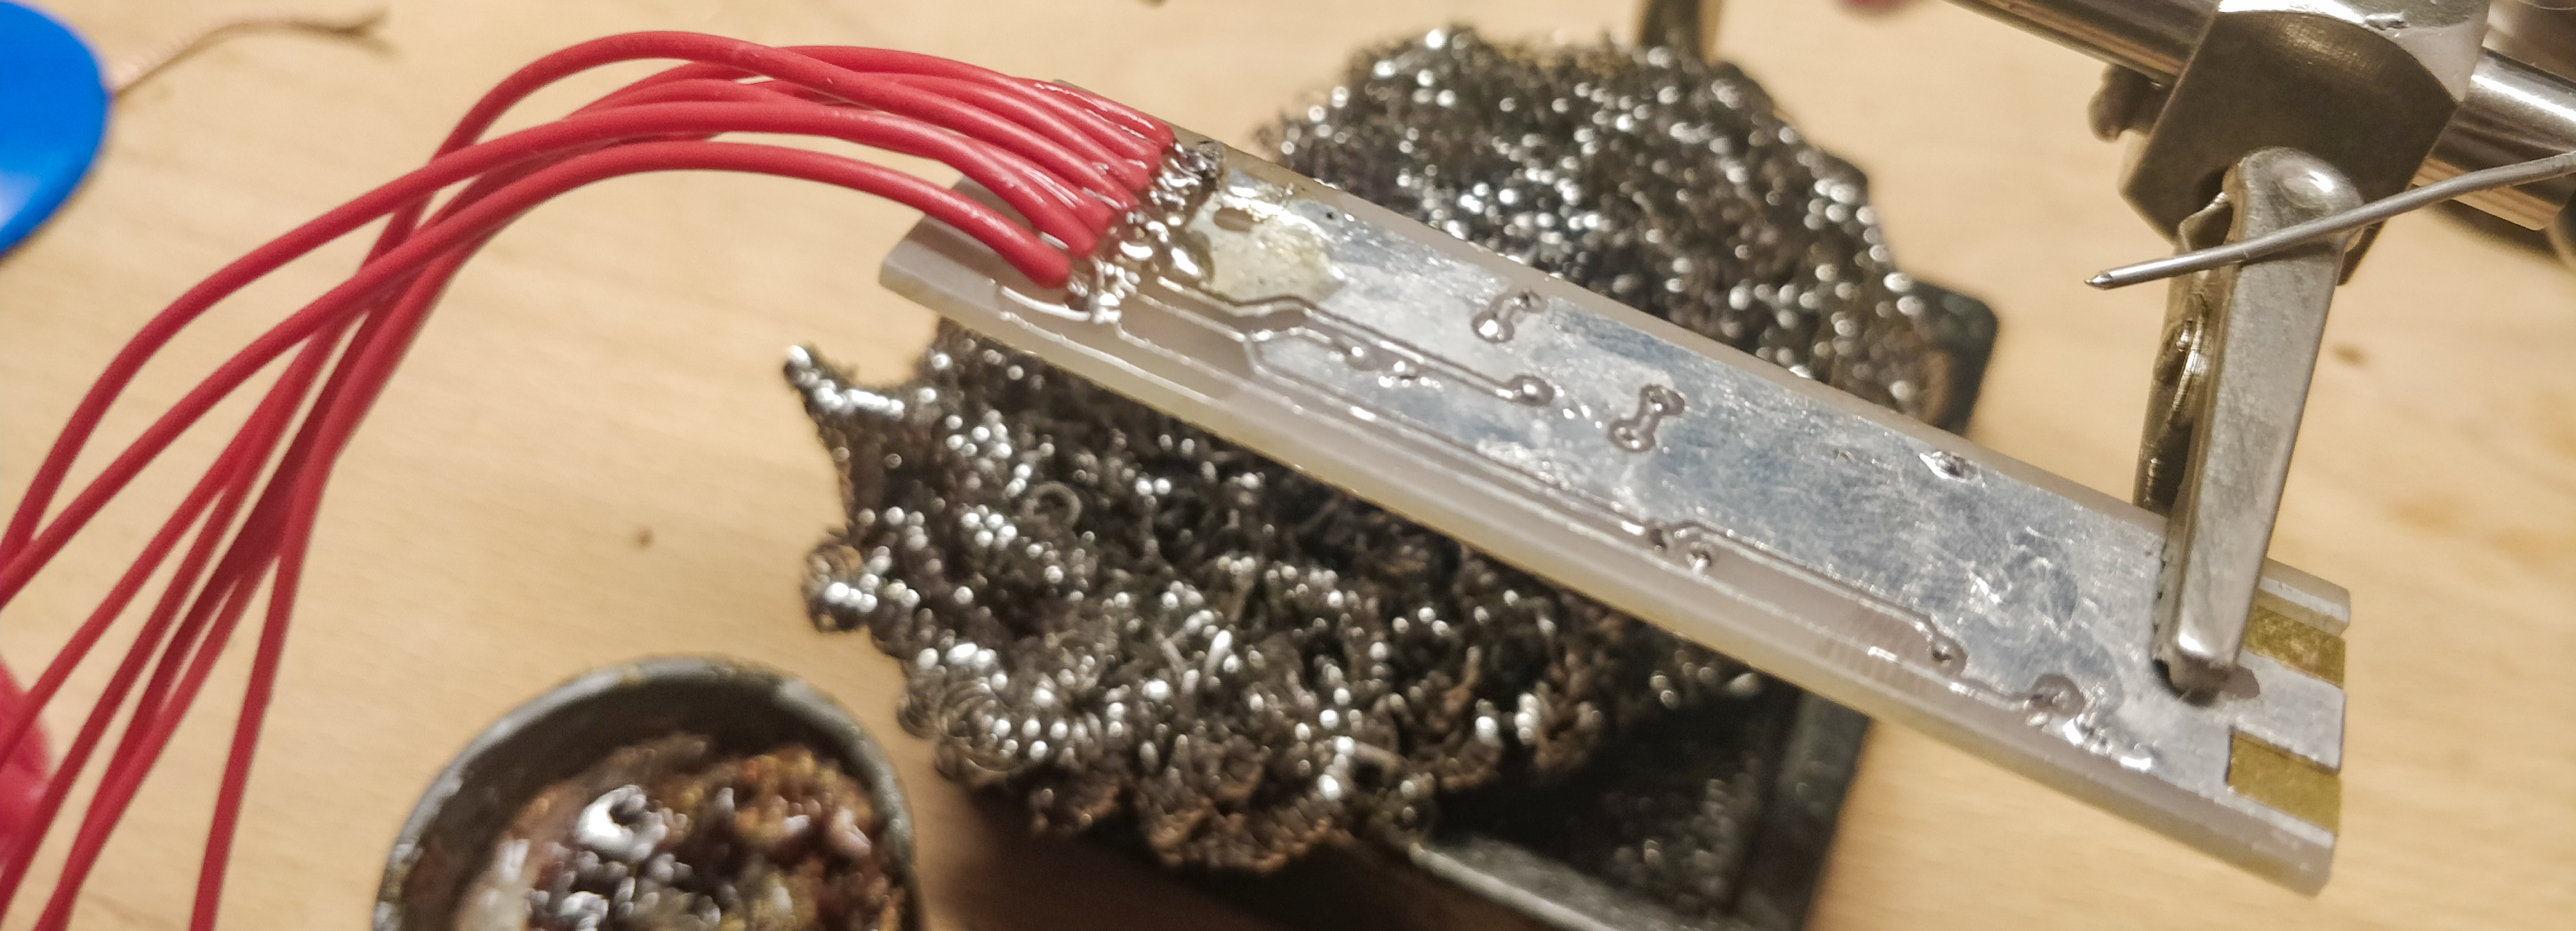
\includegraphics[width=\linewidth]{media/album/PSX_20220228_020557.jpg}
            
            \caption{}
            \label{fig:PhotoCableProgress5}
        \end{minipage}
        \\
        \vspace*{.01\linewidth}
        \begin{minipage}[H]{.95\linewidth}
            \centering
            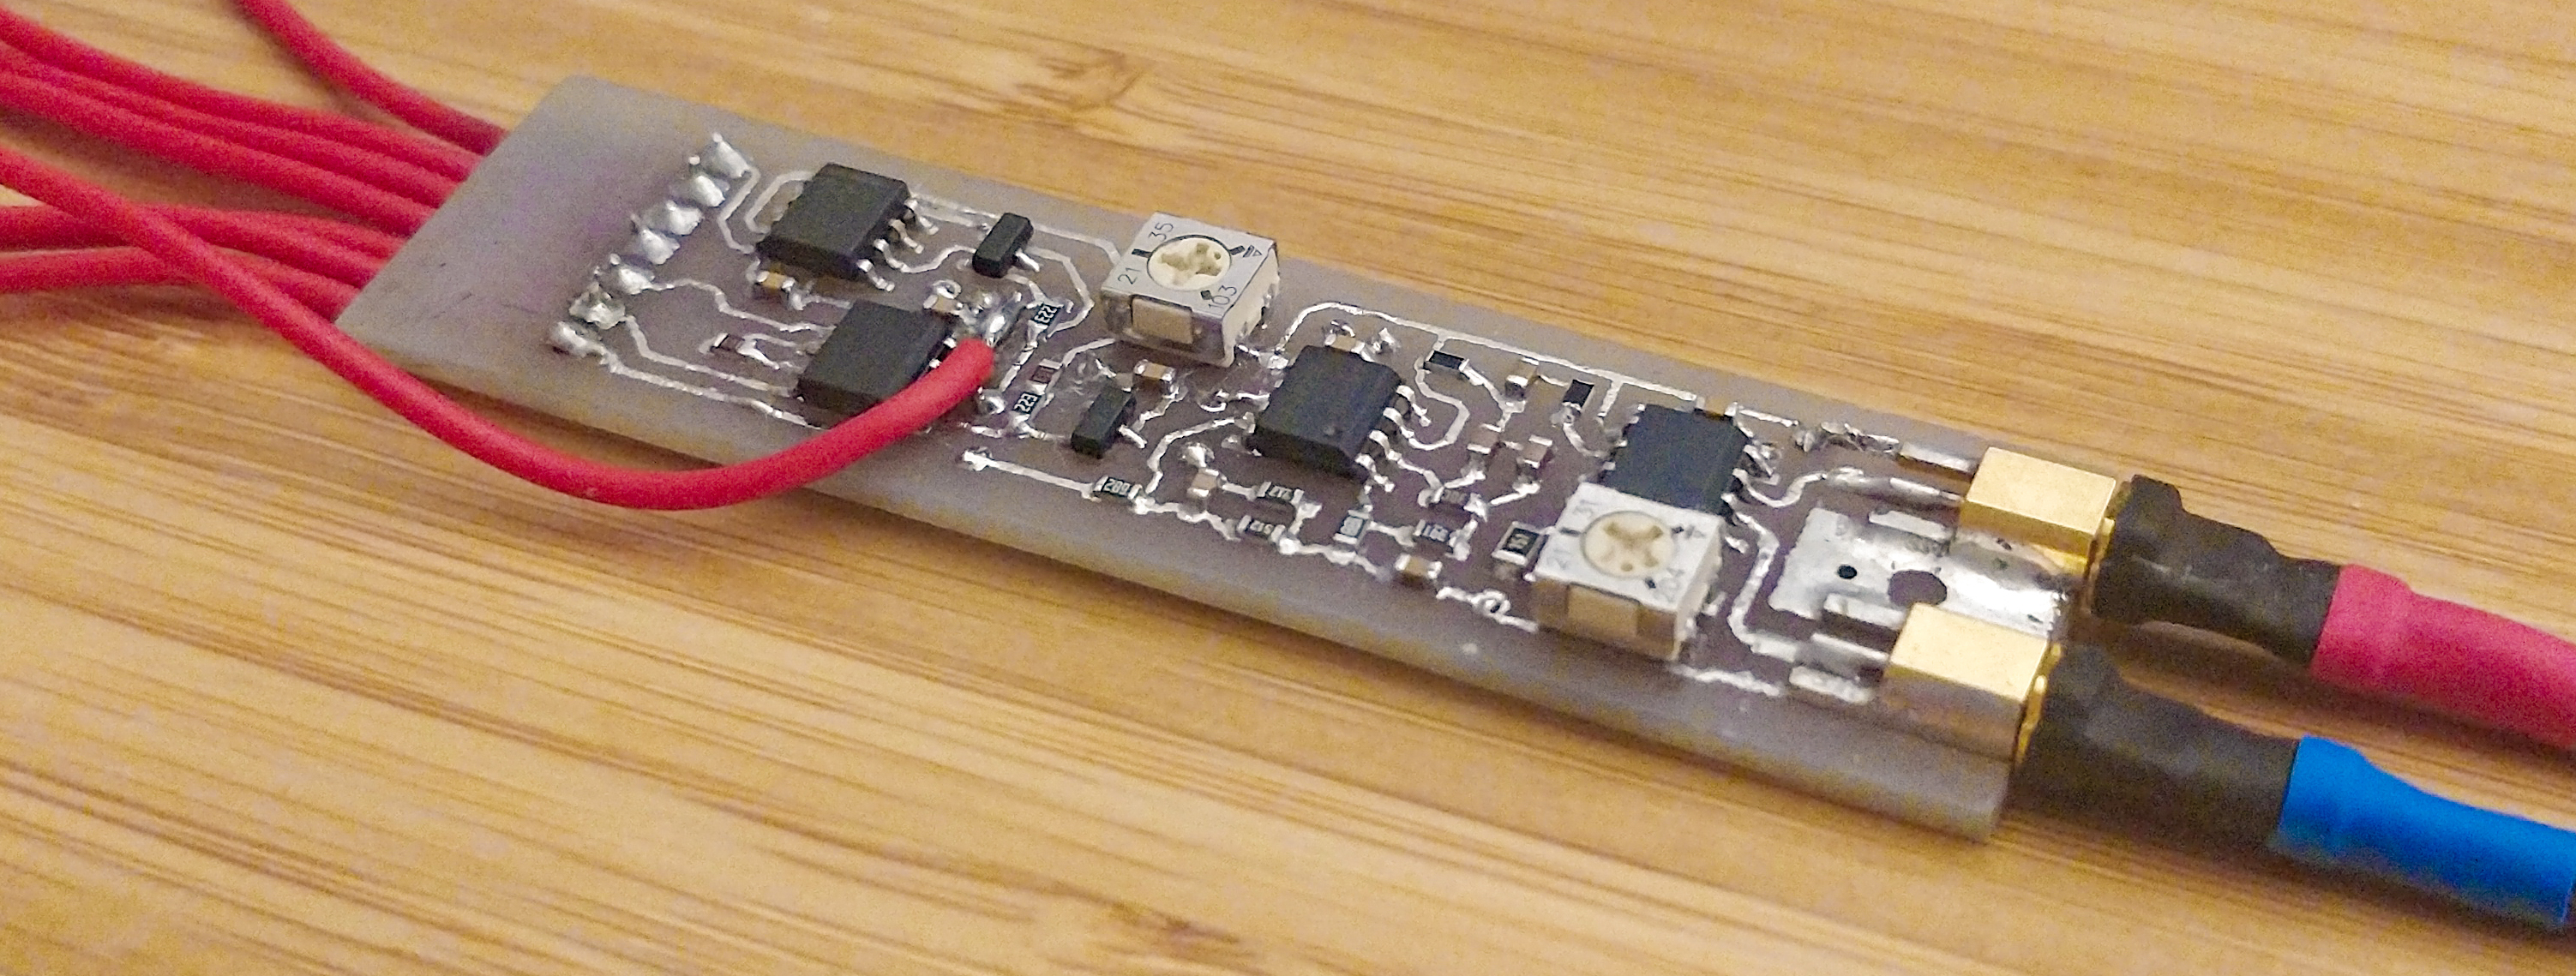
\includegraphics[width=\linewidth]{media/album/PSX_20220227_234925.jpg}
            \caption{}
            \label{fig:PhotoCableDone}
        \end{minipage}
    \end{figure}


    \subsection{Connection}
    I connected the circuit as foreseen by the schematic:
    \begin{center}
    \begin{tabular}{ ||l|l|| }
        \hline
        \multicolumn{1}{||l|}{Sensor Board} & \multicolumn{1}{|l||}{Arduino Due \& Regulator} \\
        \hline
        \hline
        CS\footnote{Chip Select} & pin 4\footnote{Any digital pin will do}\\
        \hline
        SDO\footnote{Serial Data Output} & MISO\\
        \hline
        SCLK\footnote{Serial Clock, the serial pin that sets the pace of data transmission} & SCLK\\
        \hline
        $5V$   & $5V$\\
        \hline
        $3V3$  & $3.3V$\\
        \hline
        $-3V3$ & $-3.3V$ (Regulator)\\
        \hline
        GND    & GND\\
        \hline
    \end{tabular}
    \end{center}
    \noindent Only to discover that the ADC did not work for a reason unknown to me\footnote{The ADC's SDO always stayed at "$0$": $0-20mV$}.
    So I decided to use the analog port of the Arduino DUE, with a 10bit ADC.

    \noindent The new connection is the following
    \begin{center}
        \begin{tabular}{ ||l|l|| }
            \hline
            \multicolumn{1}{||l|}{Sensor Board} & \multicolumn{1}{|l||}{Arduino Due \& Regulator} \\
            \hline
            \hline
            Output of the rectification stage\footnote{SEMG Sensor Board - RECT} & A0\footnote{The analog port of the Arduino DUE}\\
            \hline
            $5V$   & $5V$\\
            \hline
            $3V3$  & $3.3V$\\
            \hline
            $-3V3$ & $-3.3V$ (Regulator)\\
            \hline
            GND    & GND\\
            \hline
        \end{tabular}
    \end{center}

    \begin{figure}[H]
        \centering
        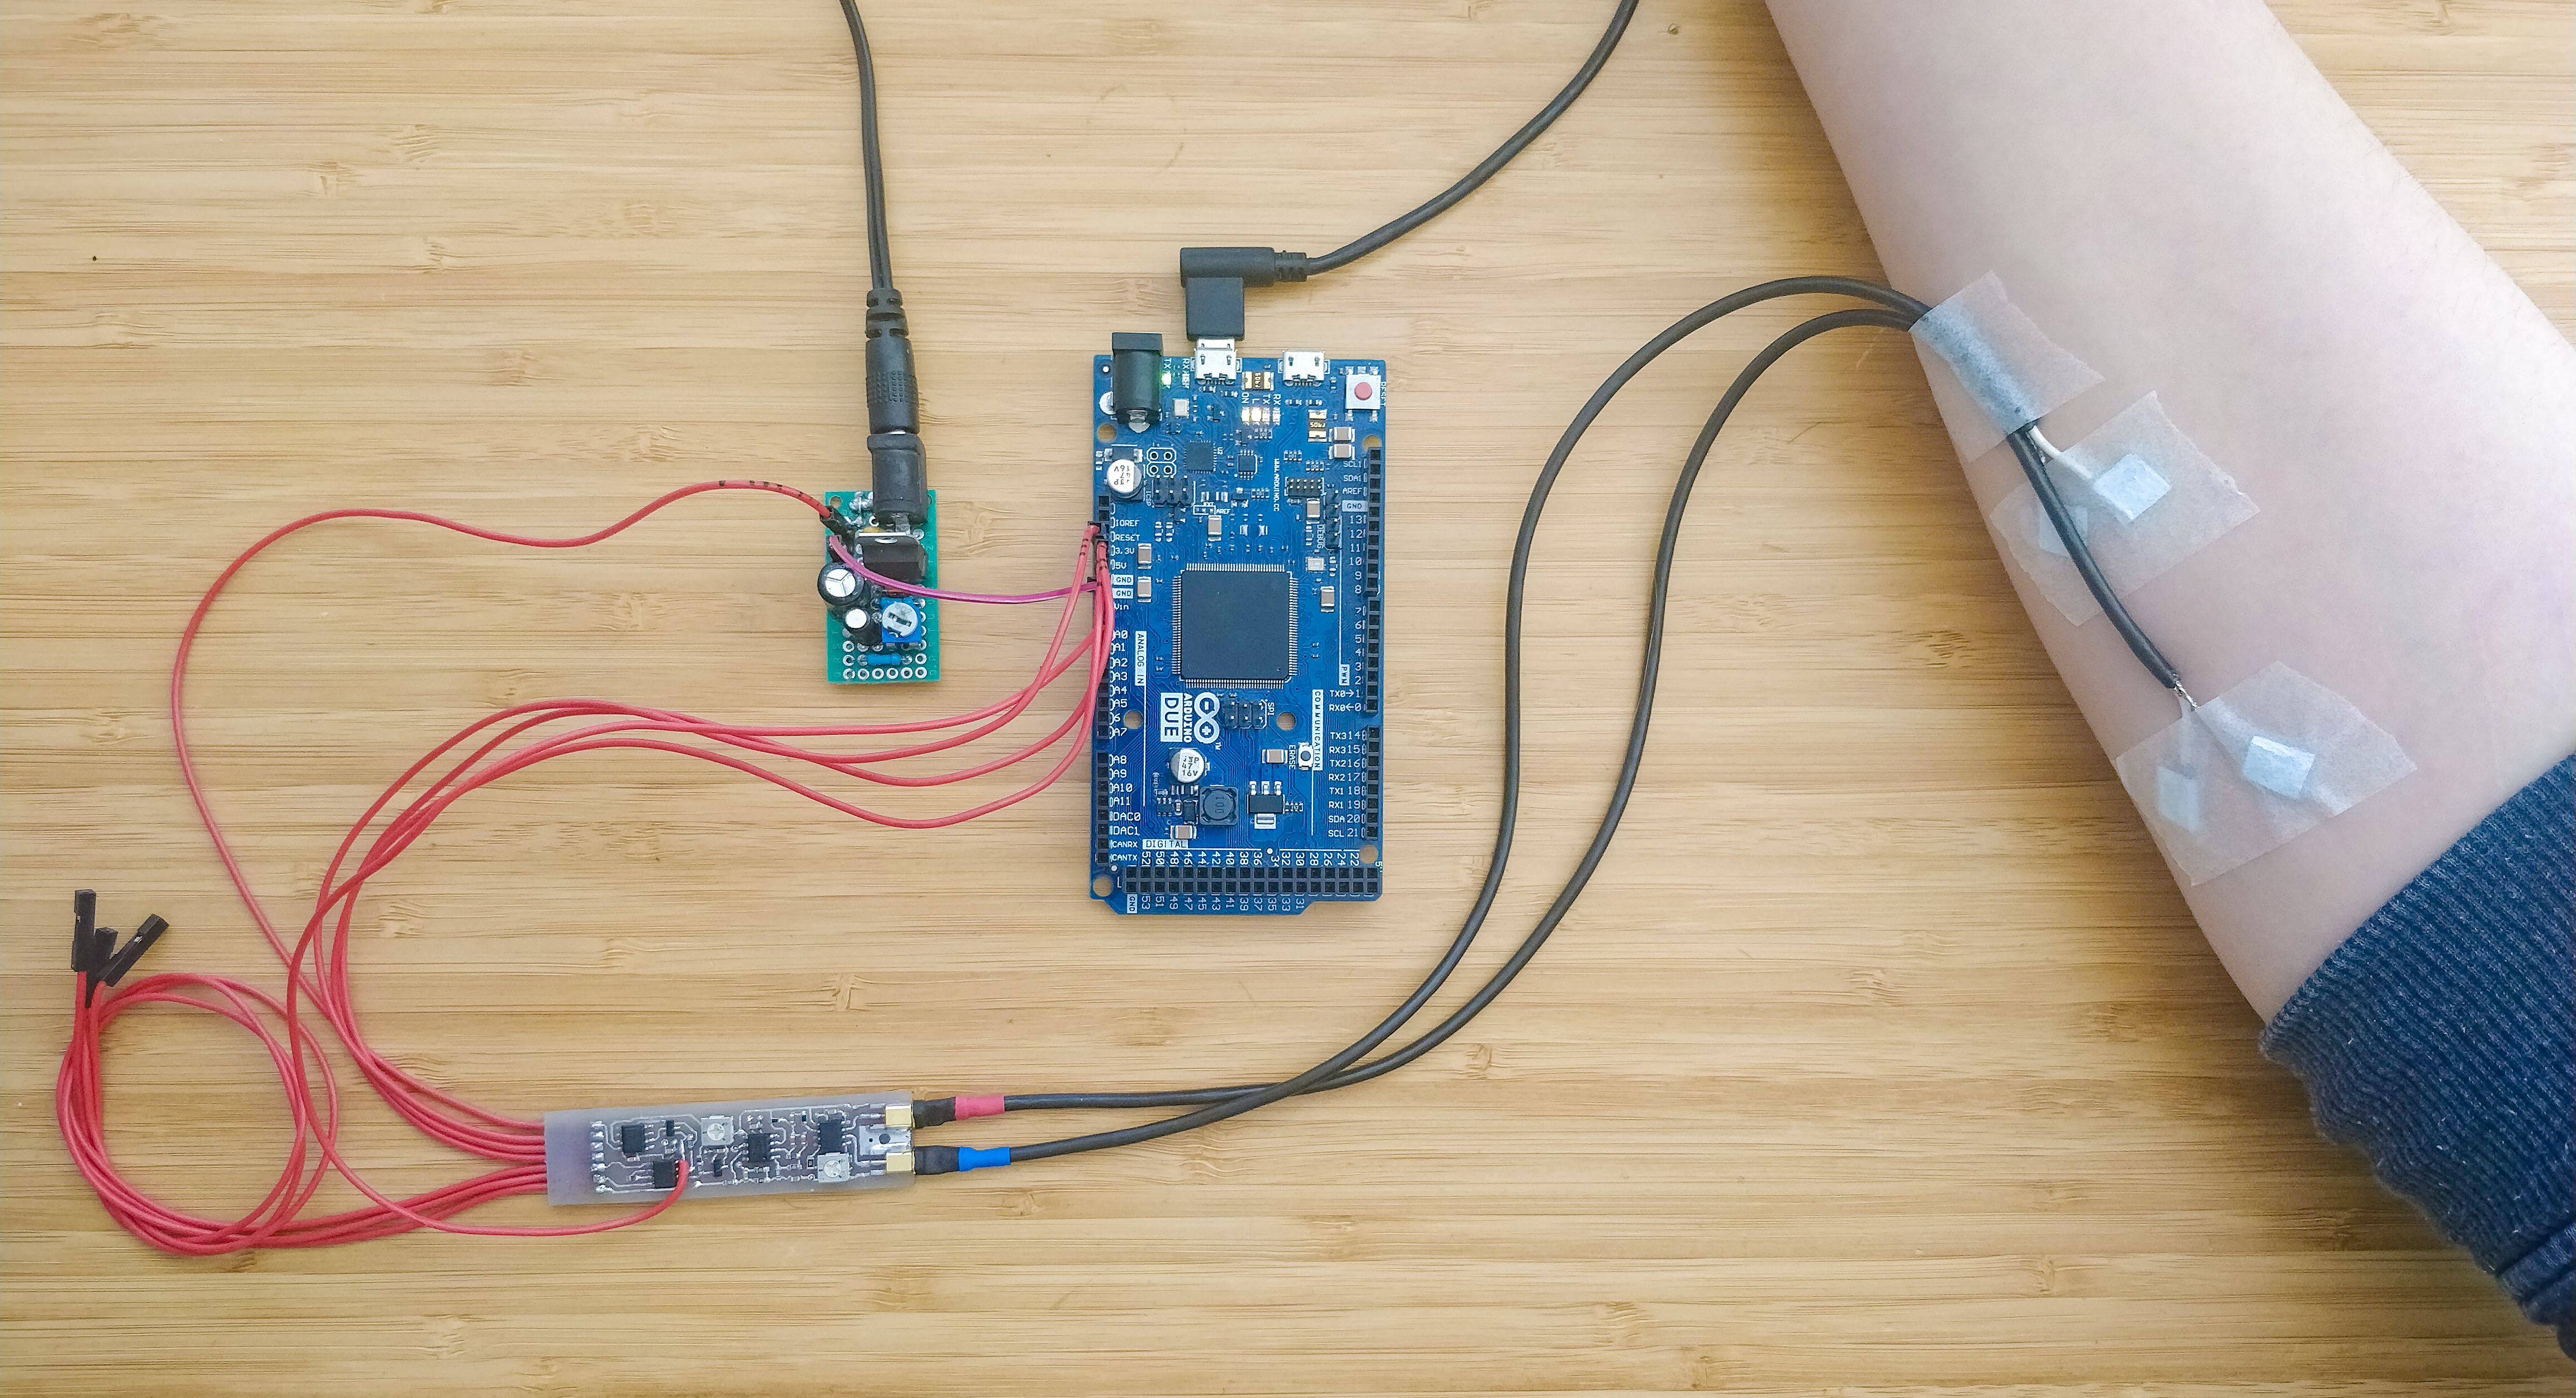
\includegraphics[width=\linewidth]{media/album/PSX_20220227_234659.jpg}
        \caption{Connection of the whole prototype}
        \label{fig:AllConnection}
    \end{figure}
    
    \subsection{Software}
    The code to communicate with the ADC via the SPI protocol:
    \begin{verbatim}
        #include <Arduino.h>            // Importa la libreria di Arudino
        #include <SPI.h>                // Importa la libreria del protocollo SPI

        /* --------------------- */
        #define SS_PIN_TLV2541  4       // Pin digitale connesso al Chip Select dell'ADC
        #define FREQ_SAMPLE 1500        // Frequenza di lettura
        /* --------------------- */

        #define DELAY_INTERSAMPLE 1000000. / FREQ_SAMPLE  // Lunghezza della pausa tra 
                                                          // le letture

        SPISettings SPI_settings_TLV2541(10000000, MSBFIRST, SPI_MODE1);  // Dichiara
                                                                // le impostazioni
                                                                // dell'ADC per l'SPI

        void setup() {
            pinMode(SS_PIN_TLV2541, OUTPUT);            // Metti il Chip Select 
                                                        // dell'ADC nella
                                                        // modalita di uscita
            Serial.begin(115200);                       // Inizializza la porta SPI
            SPI.begin();                                // Inizializza la 
                                                        // comunicazione SPI
        }

        void loop() {
            digitalWrite(SS_PIN_TLV2541, LOW);          // Attiva l'ADC
            SPI.beginTransaction(SPI_settings_TLV2541); // Inizia trasmissione dati
                                                        // con impostazioni
                                                        // dell'ADC
            uint16_t val = SPI.transfer16(0x00);        // Leggi il valore in una
                                                        // variabile di 16 bit senza
                                                        // segno
            delayMicroseconds(4);                       // Dai del tempo all'ADC
                                                        // per convertire il segnale
            SPI.endTransaction();                       // Finisci trasmissione dati
            digitalWrite(SS_PIN_TLV2541, HIGH);         // Disabilita l'ADC

            Serial.println(val);                        // Stampa il valore nella porta
                                                        // seriale
            delayMicroseconds(DELAY_INTERSAMPLE);       // Aspetta il tempo predefinito
        }
    \end{verbatim}

    \noindent The current code to read the value from analog port A0
    \begin{verbatim}
        #include <Arduino.h>          // Importa la libreria di Arudino

        /* --------------------- */
        #define SENSE_PIN A0          // Pin analogico
        #define FREQ_SAMPLE 1500      // Frequenza di lettura
        /* --------------------- */

        #define DELAY_INTERSAMPLE 1000000. / FREQ_SAMPLE  // Lunghezza della pausa tra
                                                          //le letture

        void setup() {
            Serial.begin(115200); // Inizia la comunicazione seriale
        }

        void loop() {
            Serial.println(analogRead(SENSE_PIN));  // Leggi il valore dal pin 
                                                    // analogico e invialo
                                                    // alla porta seriale
            delayMicroseconds(DELAY_INTERSAMPLE);   // Aspetta il tempo predefinito
        }
    \end{verbatim}

    To display the plot I used the following existing program written in Processing \parenciteit{}{ProcessingGrapher:Software}
    \section{Results} \label{sec:Results}
    \begin{figure}[H]
        \centering
        \begin{minipage}[H]{\linewidth}
            \begin{tikzpicture}
                \begin{axis}[
                    axis x line=bottom,
                    axis y line*=left,
                    ylabel style={rotate=-90},
                    xlabel={$t[ms]$},
                    ylabel={$U[V]\cdot k$},
                    legend entries={$($Channel $1)$},
                    legend pos=north east,
                    height=.4\textwidth,
                    width=.85\textwidth,
                    smooth,
                    clip=true,
                    xmin=0,
                    % xmax=17500,
                    colormap/twilight_shifted,
                    axis_style_default_data,
                    ymajorgrids=true,
                    xmajorgrids=false,
                    grid style=dashed,
                    cycle list={[colors of colormap={145,250},]},
                    every axis plot/.append style={mark=none, thick, draw opacity=.7},
                    ]
                    % [2026 revision] measured signal in solid dark teal (was twilight_shifted
                    % mid-range + draw opacity .7; user request: clearer "real measured" color)
                    \addplot[draw=teal!70!black, draw opacity=1] table [header=false, col sep=comma]{datasets/result/gr1.csv};
                \end{axis}
            \end{tikzpicture}
            \subcaption{Demonstration that the signal can be read}
        \end{minipage}
        \begin{minipage}[H]{\linewidth}
            \begin{tikzpicture}
                \begin{axis}[
                    axis x line=bottom,
                    axis y line*=left,
                    ylabel style={rotate=-90},
                    xlabel={$t[ms]$},
                    ylabel={$U[V]\cdot k$},
                    legend entries={$($Channel $1)$},
                    legend pos=north east,
                    height=.4\textwidth,
                    width=.85\textwidth,
                    smooth,
                    clip=true,
                    xmin=0,
                    % xmax=17500,
                    colormap/twilight_shifted,
                    axis_style_default_data,
                    ymajorgrids=true,
                    xmajorgrids=false,
                    grid style=dashed,
                    cycle list={[colors of colormap={145,250},]},
                    every axis plot/.append style={mark=none, thick, draw opacity=.7},
                    ]
                    \addplot[draw=teal!70!black, draw opacity=1] table [header=false, col sep=comma]{datasets/result/gr2.csv};
                \end{axis}
            \end{tikzpicture}
            \subcaption{Demonstration that the signal amplitude can be adjusted \emph{(The first three muscle contractions are at one amplification threshold, while the next two are at another one that is clearly lower)}}
        \end{minipage}
        \begin{minipage}[H]{\linewidth}
            \begin{tikzpicture}
                \begin{axis}[
                    axis x line=bottom,
                    axis y line*=left,
                    ylabel style={rotate=-90},
                    xlabel={$t[ms]$},
                    ylabel={$U[V]\cdot k$},
                    legend entries={$($Channel $1)$},
                    legend pos=north east,
                    height=.4\textwidth,
                    width=.85\textwidth,
                    smooth,
                    clip=true,
                    xmin=0,
                    % xmax=17500,
                    colormap/twilight_shifted,
                    axis_style_default_data,
                    ymajorgrids=true,
                    xmajorgrids=false,
                    grid style=dashed,
                    cycle list={[colors of colormap={145,250},]},
                    every axis plot/.append style={mark=none, thick, draw opacity=.7},
                    ]
                    \addplot[draw=teal!70!black, draw opacity=1] table [header=false, col sep=comma]{datasets/result/gr3.csv};
                \end{axis}
            \end{tikzpicture}
            % TRANSLATOR NOTE: "altezza del segnale" (height of the signal) most likely means the DC offset set by RV2; kept literal.
            \subcaption{Demonstration that the height of the signal can be adjusted}
        \end{minipage}
        \caption{Sampled signals from the sensor board during a series of hand contractions \emph{(A larger signal means the muscle is contracting)}}
    \end{figure}
    Having shown this, I can consider the goal of the \emph{maturit\`{a}} thesis achieved.

    \section{Conclusions}
    I consider this prototype a success, both as a proof that it works and for the great deal of knowledge I acquired during the research.
    Despite some small mistakes\footnote{Such as the non-working ADC} that prevented me from verifying other factors, such as the noise introduced by the circuit and the appropriate amplification of the signal, I managed to filter the signal adequately and obtain a fairly clean signal.
    The numerous difficulties I encountered during the design of the project, ranging from problems with the computer's operating system to time lost on the internet searching for very scattered information, have made me more confident in my abilities and my problem-solving methods.
    % TRANSLATOR NOTE: original has a typo "e non e molto piu vasto"; read as "is not much larger".
    The work still to be done to obtain a working skateboard is not much larger than the work I did during this \emph{maturit\`{a}} thesis, because I believe that designing analog signal-processing circuits is one of the most complex things in all of electrical engineering.
    I am also glad that my project was done with future plans in mind, even though this part took a lot of my time: for example, the gain adjustment can easily be replaced by a digital potentiometer\footnote{A component that varies its resistance via digital communication protocols} to obtain a self-calibration feature, and the low current drawn by the circuit\footnote{This part is also included in the calculations} lets me choose how sophisticated to make the circuit thanks to the spare battery capacity (or to shrink the circuit even further without fearing that it will overheat).
    Finally, I am happy not only with the work I did, but also with how it was done: by myself, with my own hands and my own mind.

    \section{Calculations} \label{sec:Calculations}
    In this Section I present various documents I obtained while using Maple to calculate different results.
    \begin{center}
        \begin{tabular}{ ||l|l|| }
            \hline
            \multicolumn{1}{||l|}{Title} & \multicolumn{1}{|l||}{Topic} \\
            \hline
            \hline
            LPF Theor Model & Theoretical model of the transfer function of an LPF \\
            HPF Theor Model & Theoretical model of the transfer function of an HPF \\
            Transfer Function Derivation & Derivation of the transfer functions \\
            Voltage Regulator & Information about the voltage regulator \\
            Voltage Reference & Information about the voltage reference \\
            Offset Amplification Tuning & Tuning of the gain distribution across the circuit stages \\
            Noise & Calculation of the noise introduced by the circuit \\
            INA & Information about the INA \\
            OA & Information about the OA \\
            ADC & Information about the ADC \\
            \hline
        \end{tabular}
    \end{center}

    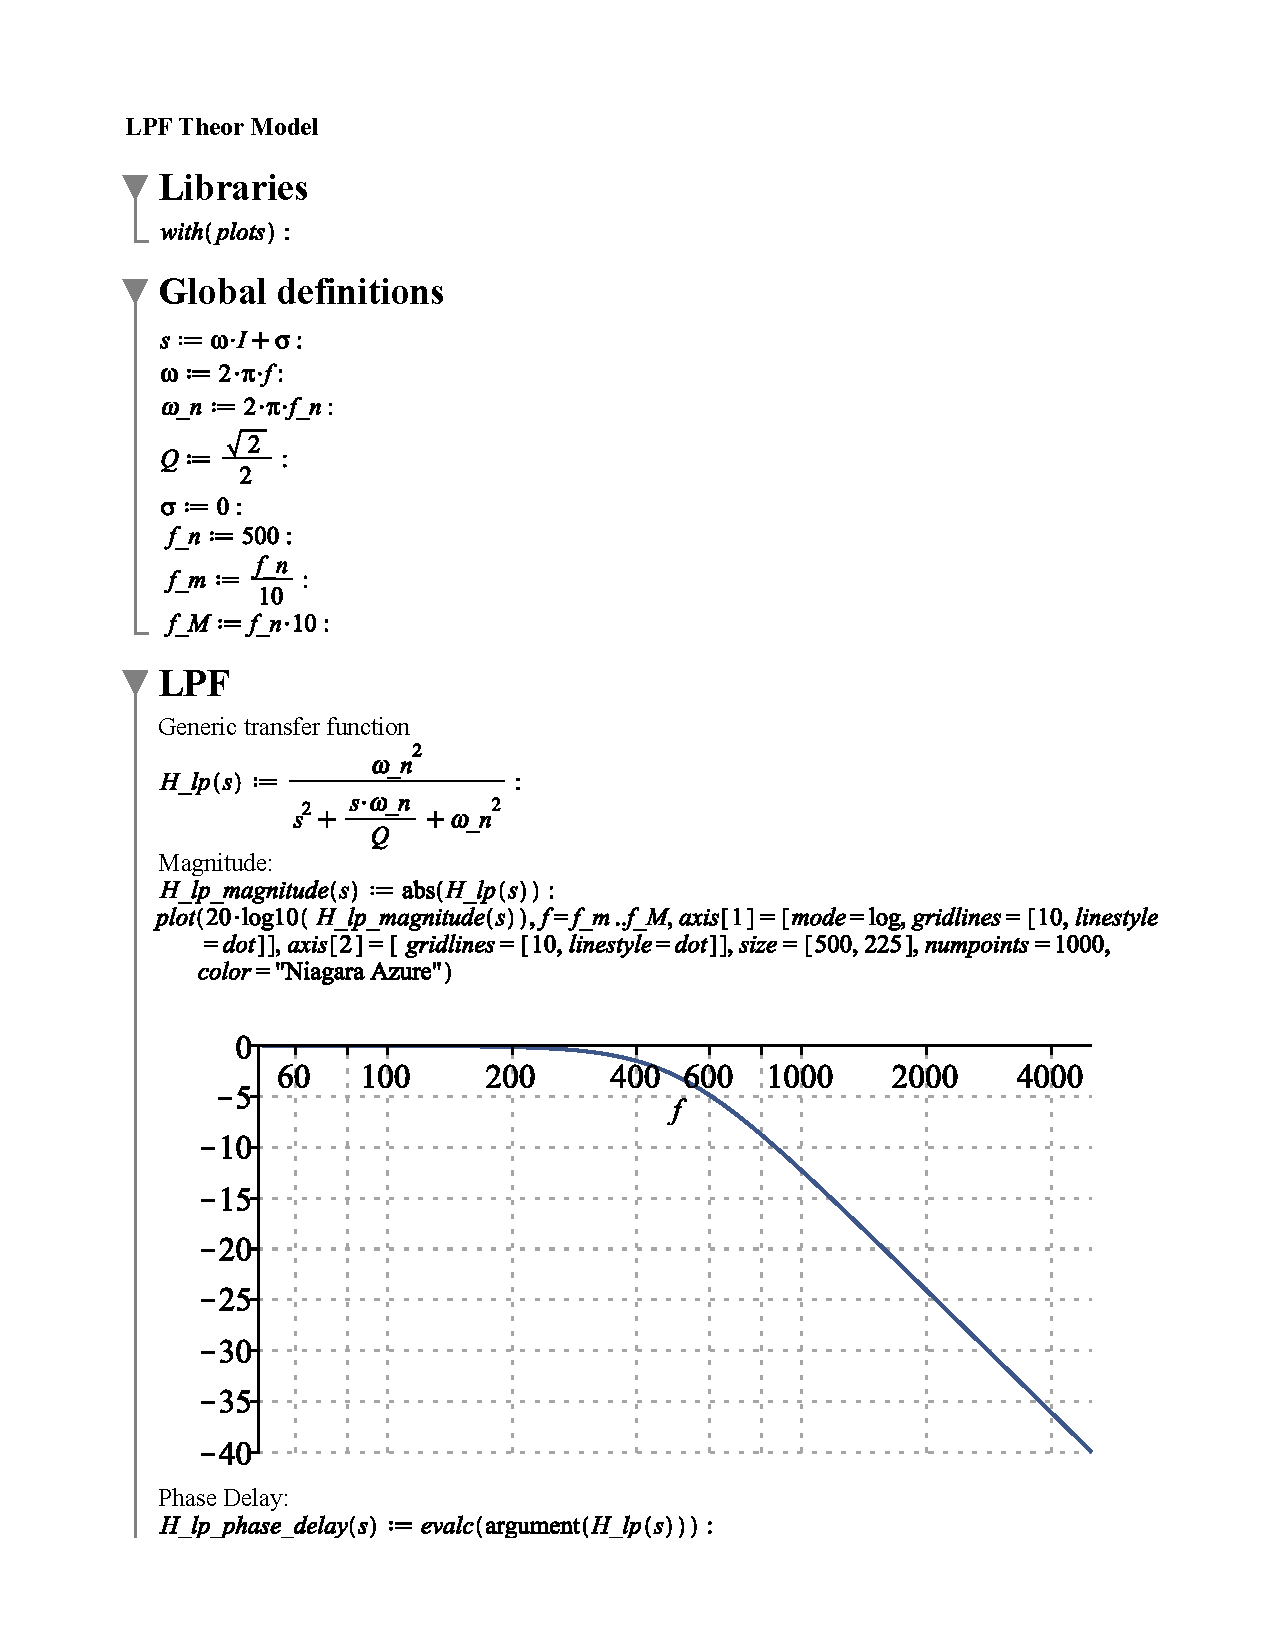
\includepdf[pages=-]{media/maple/lpf_theor-model.pdf}
    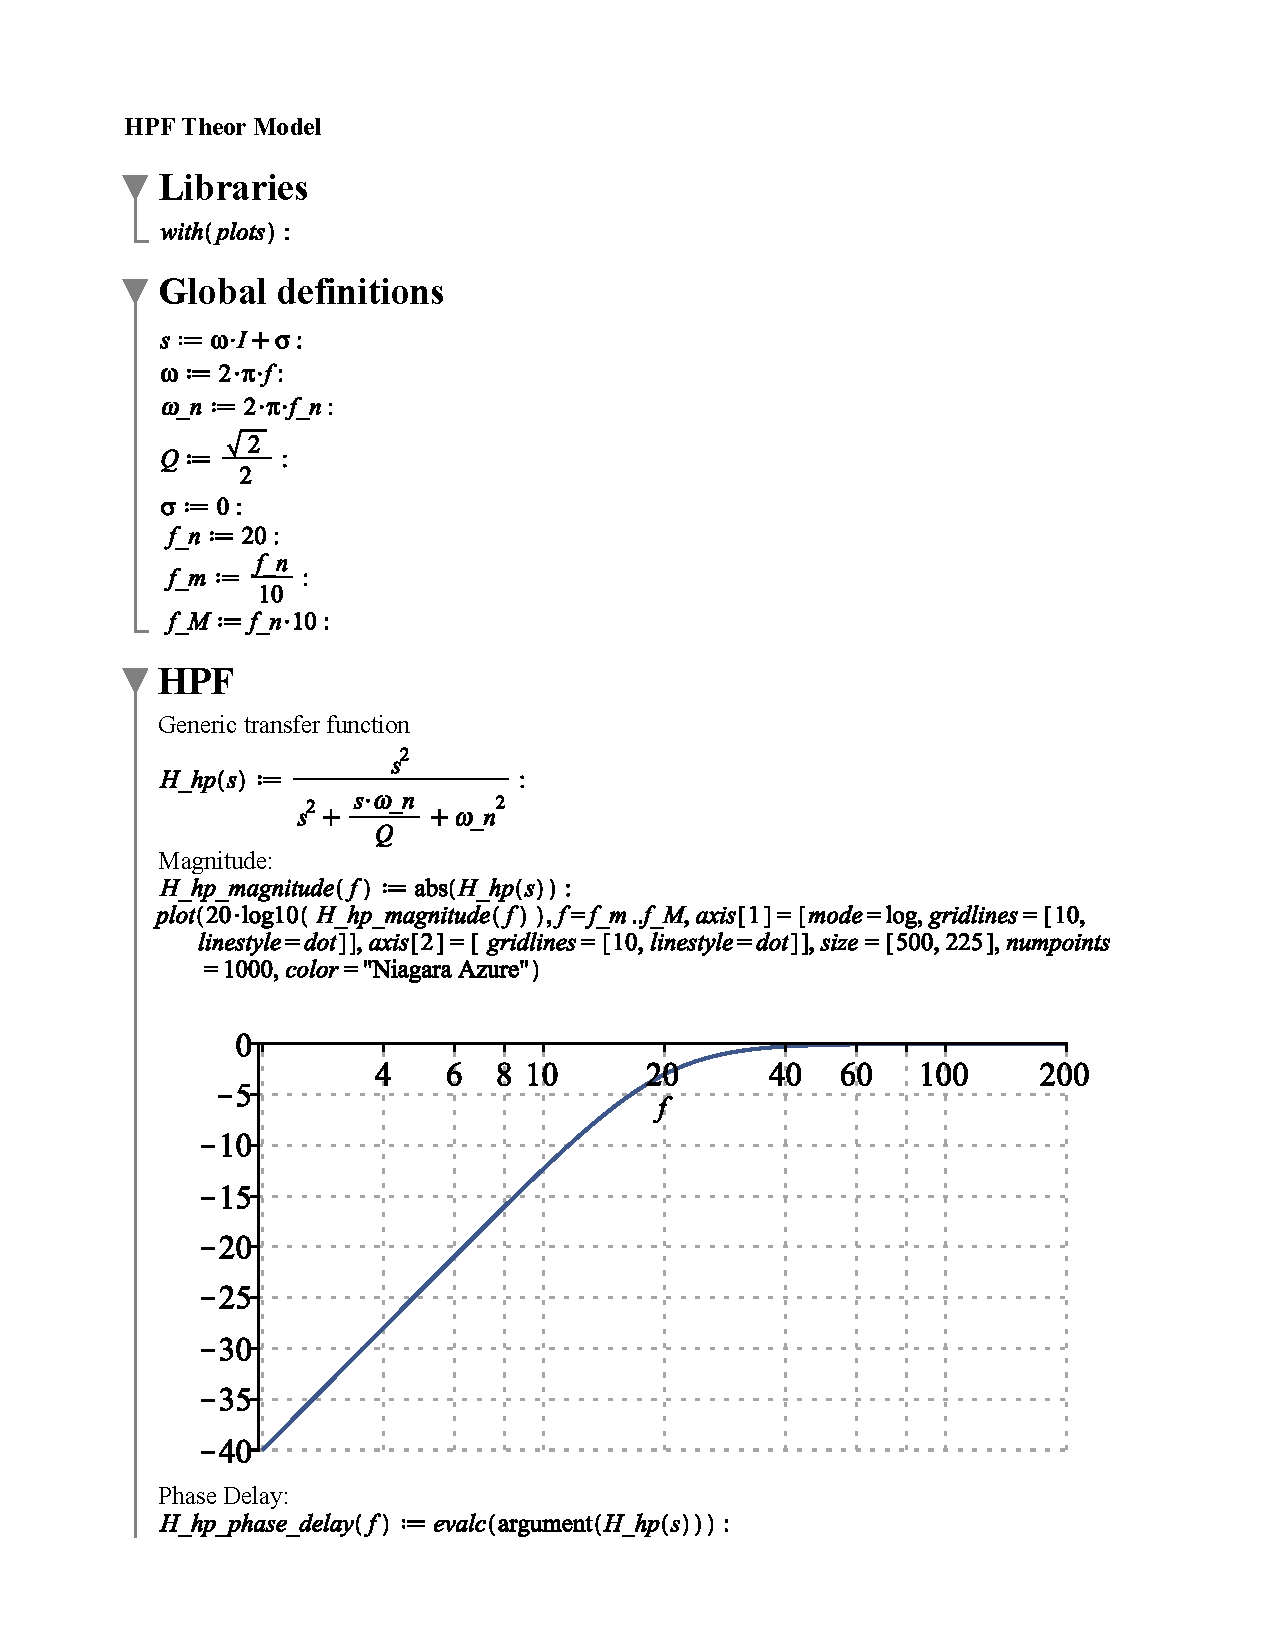
\includepdf[pages=-]{media/maple/hpf_theor-model.pdf}
    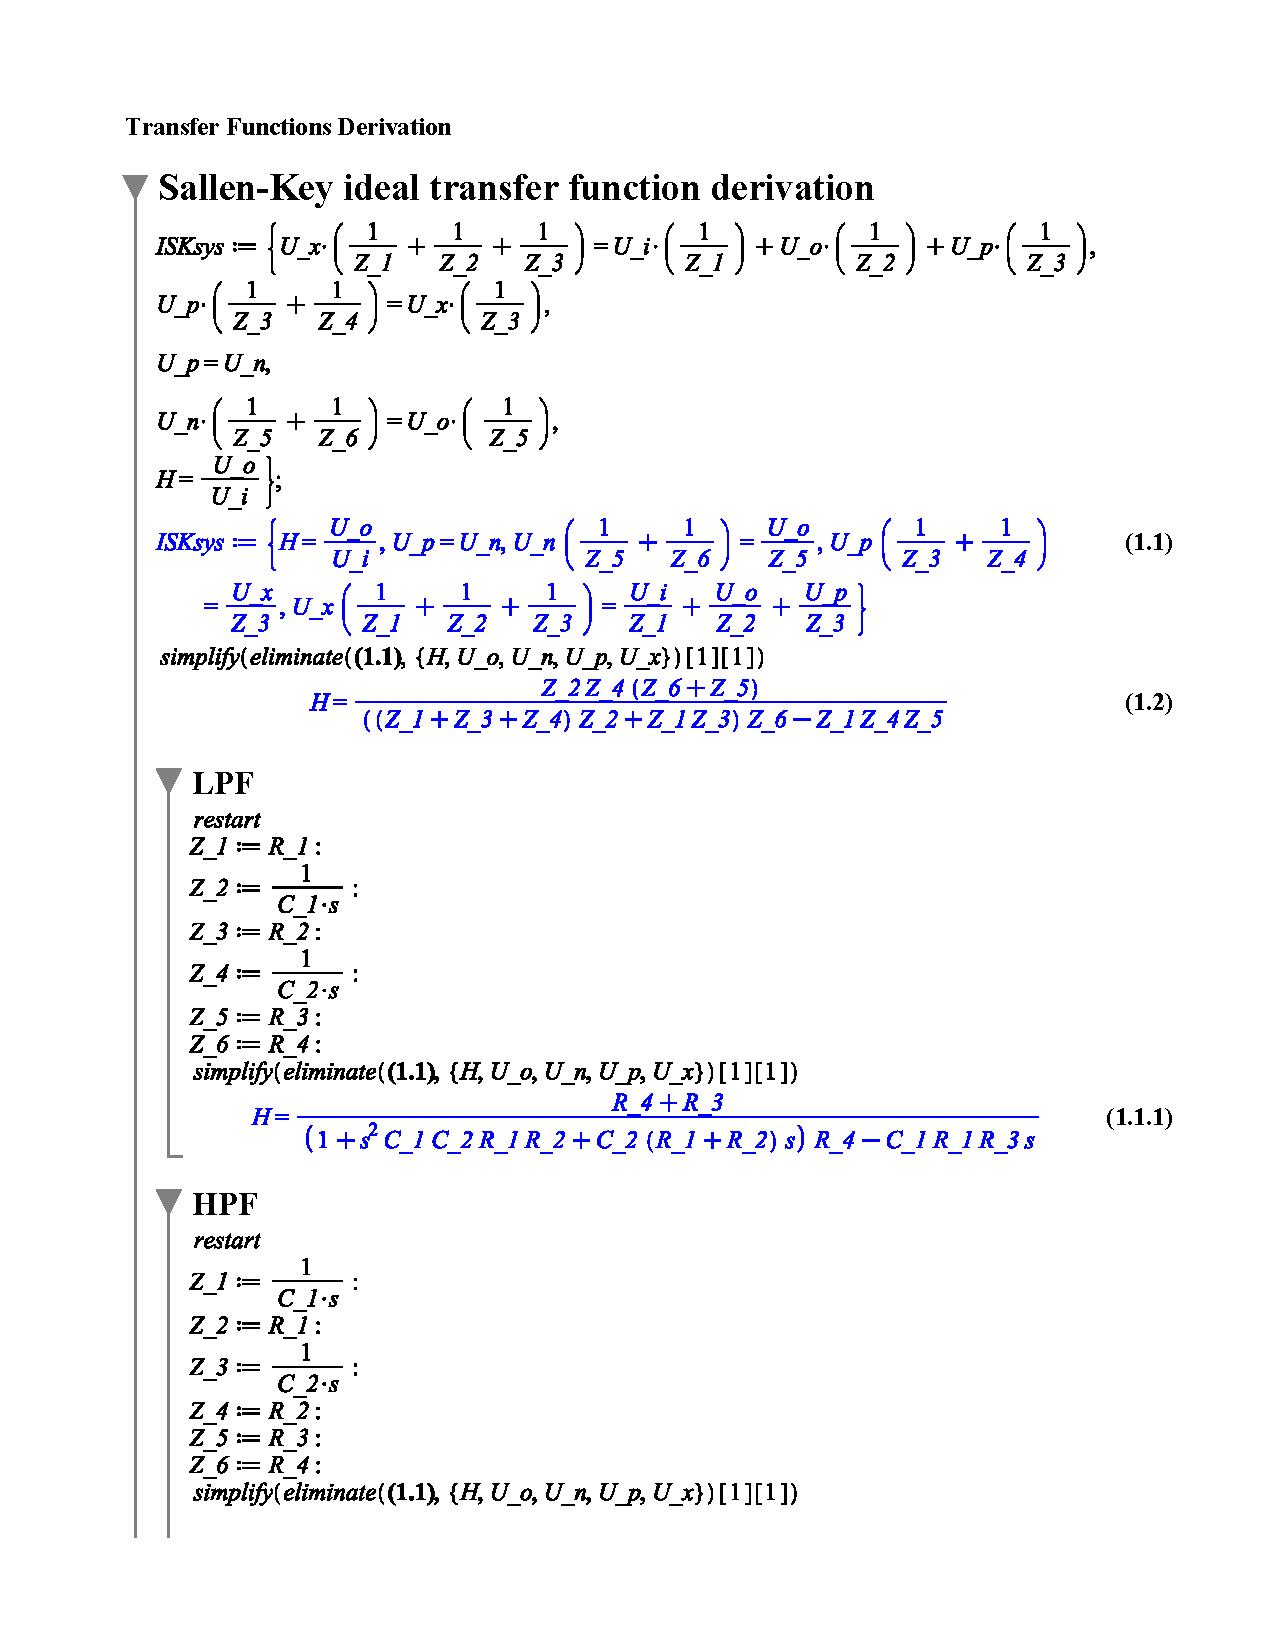
\includepdf[pages=-]{media/maple/tranfer_functions_derivation.pdf}
    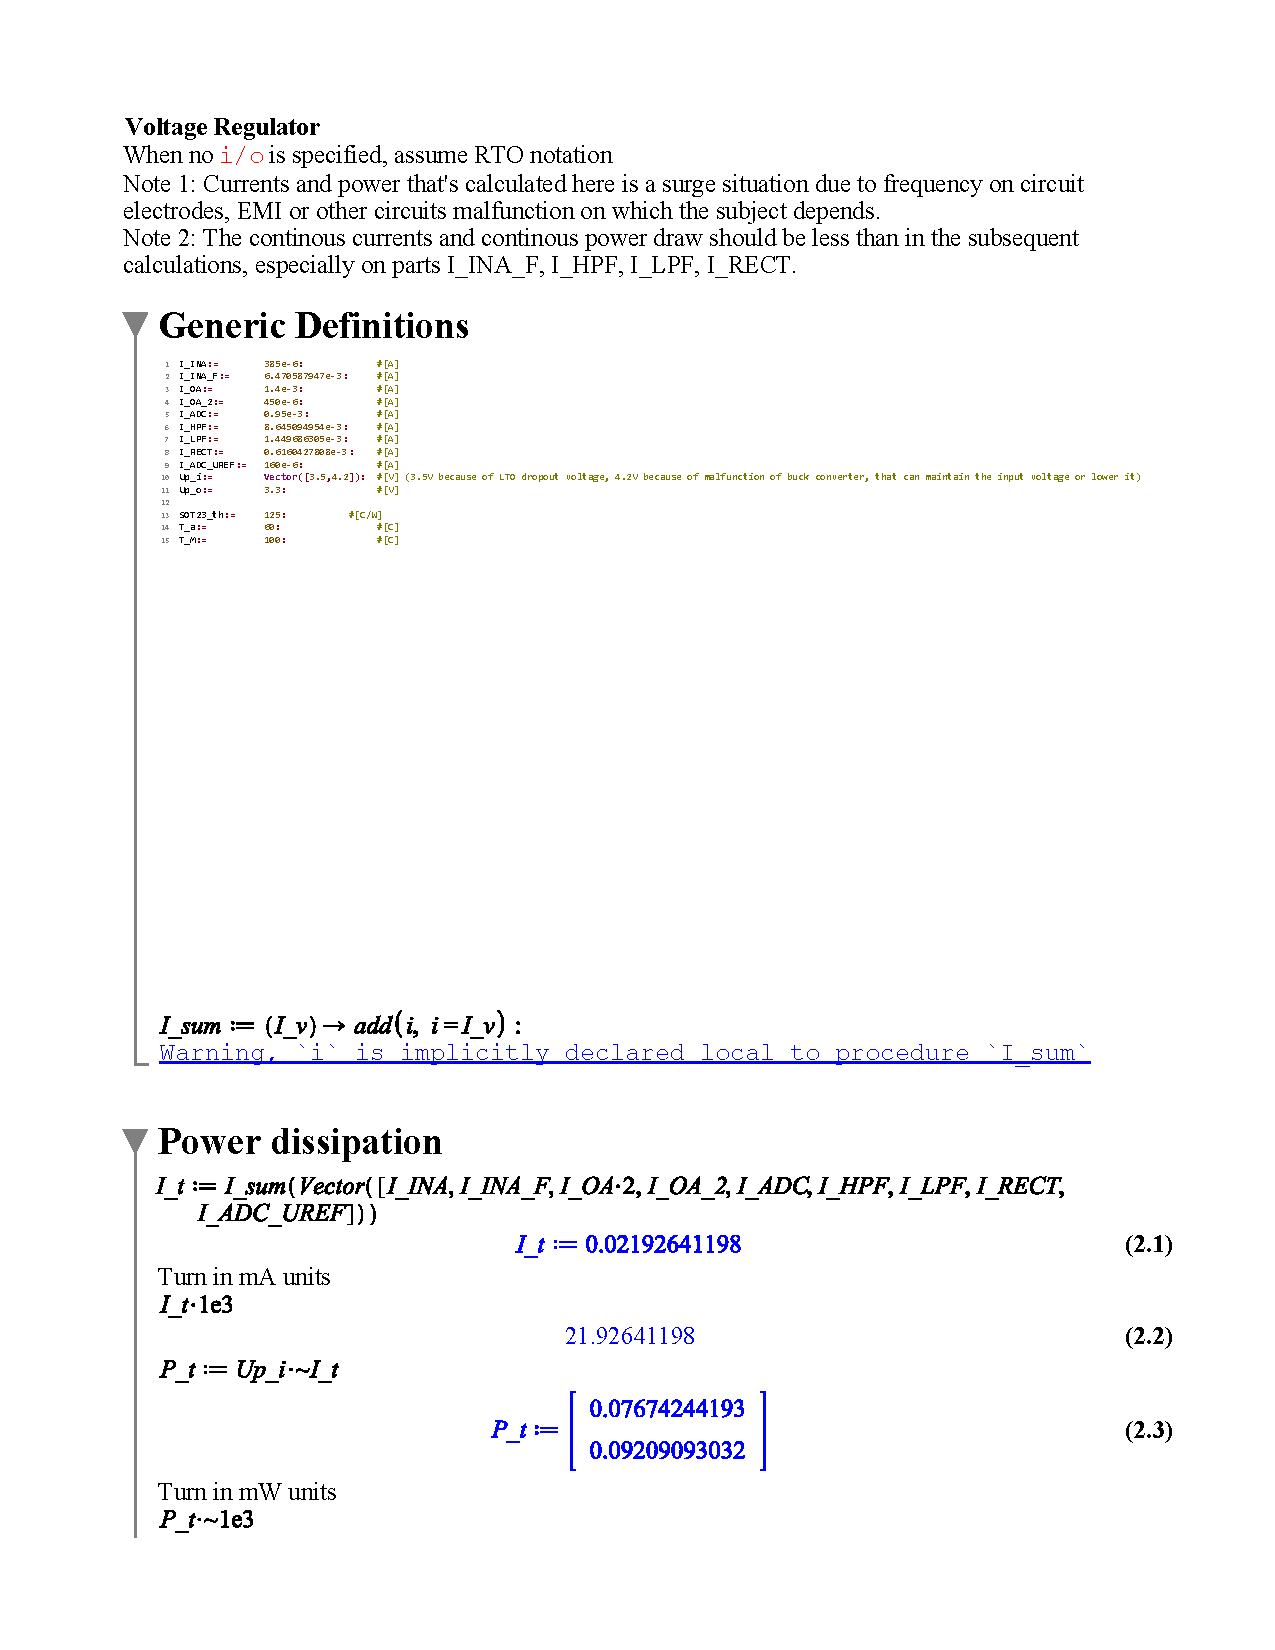
\includepdf[pages=-]{media/maple/voltage_regulator.pdf}
    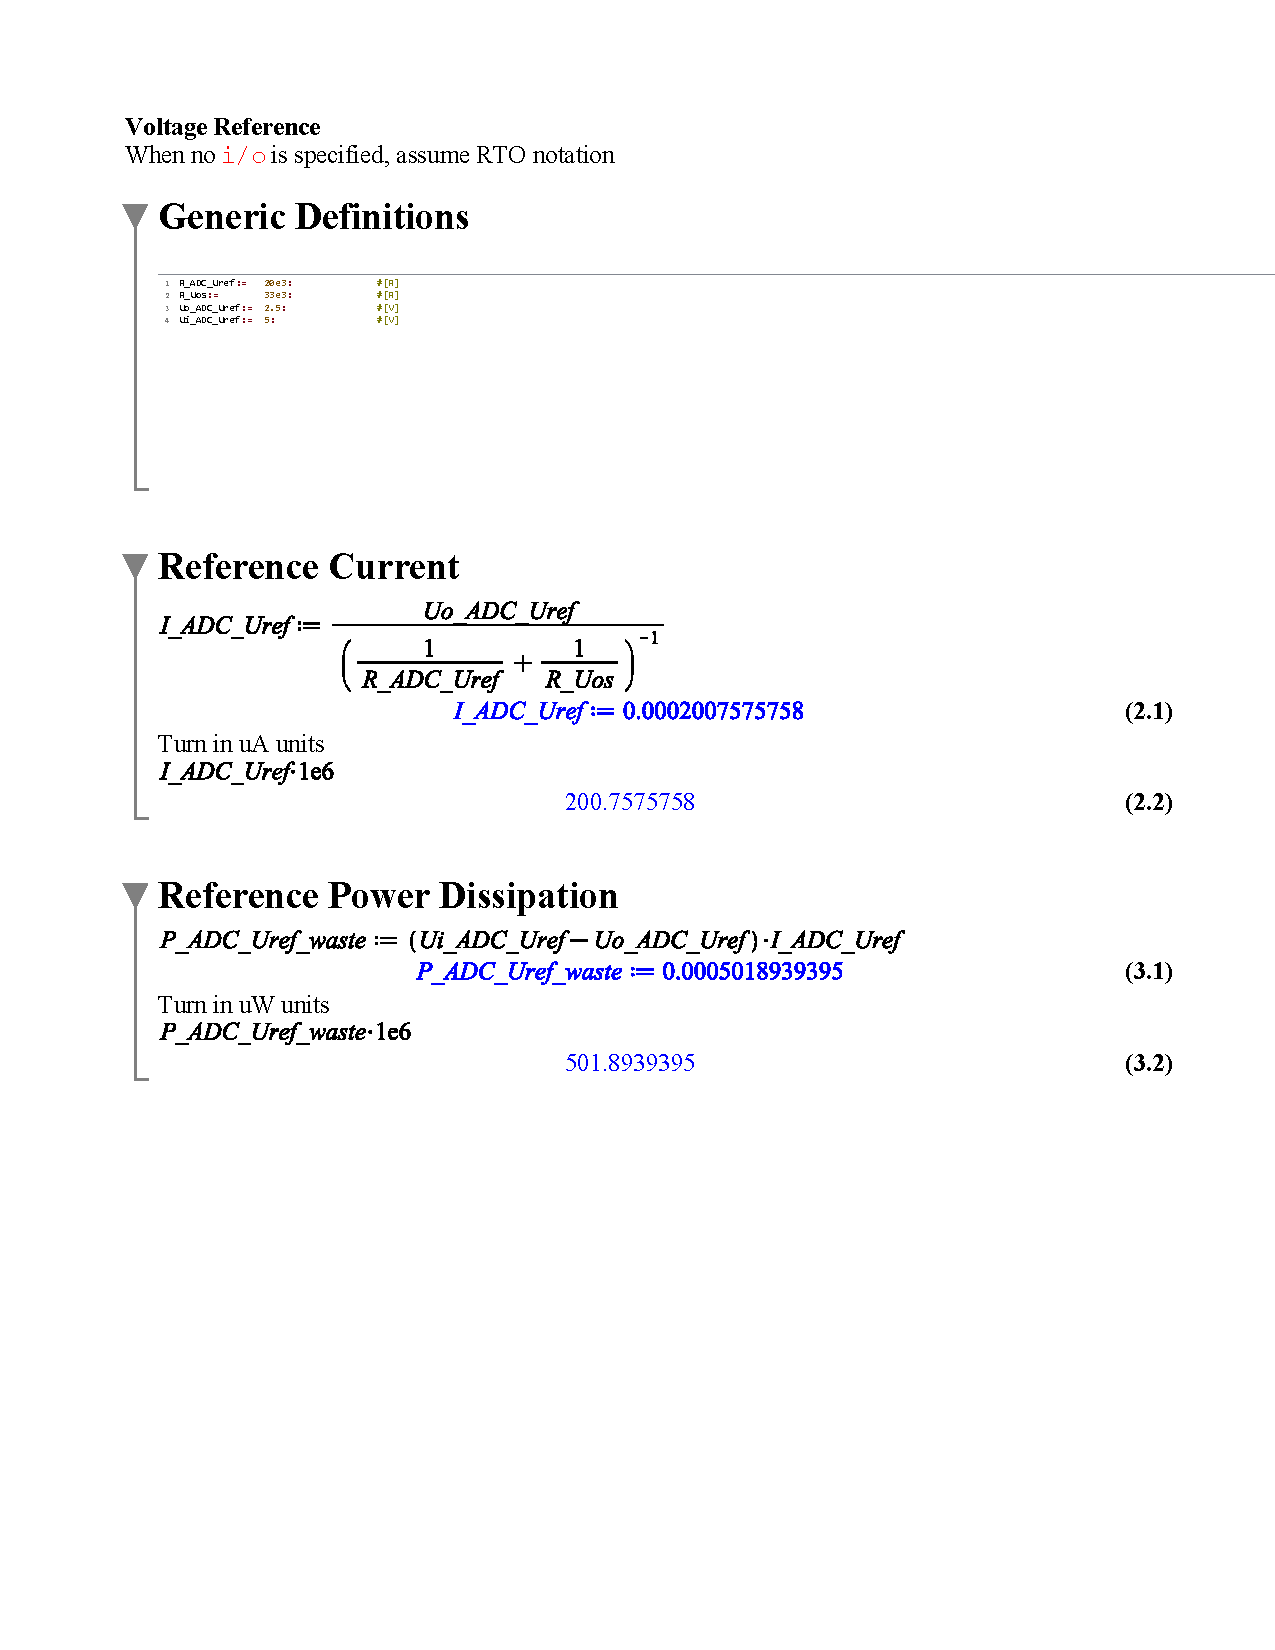
\includepdf[pages=-]{media/maple/voltage_reference.pdf}
    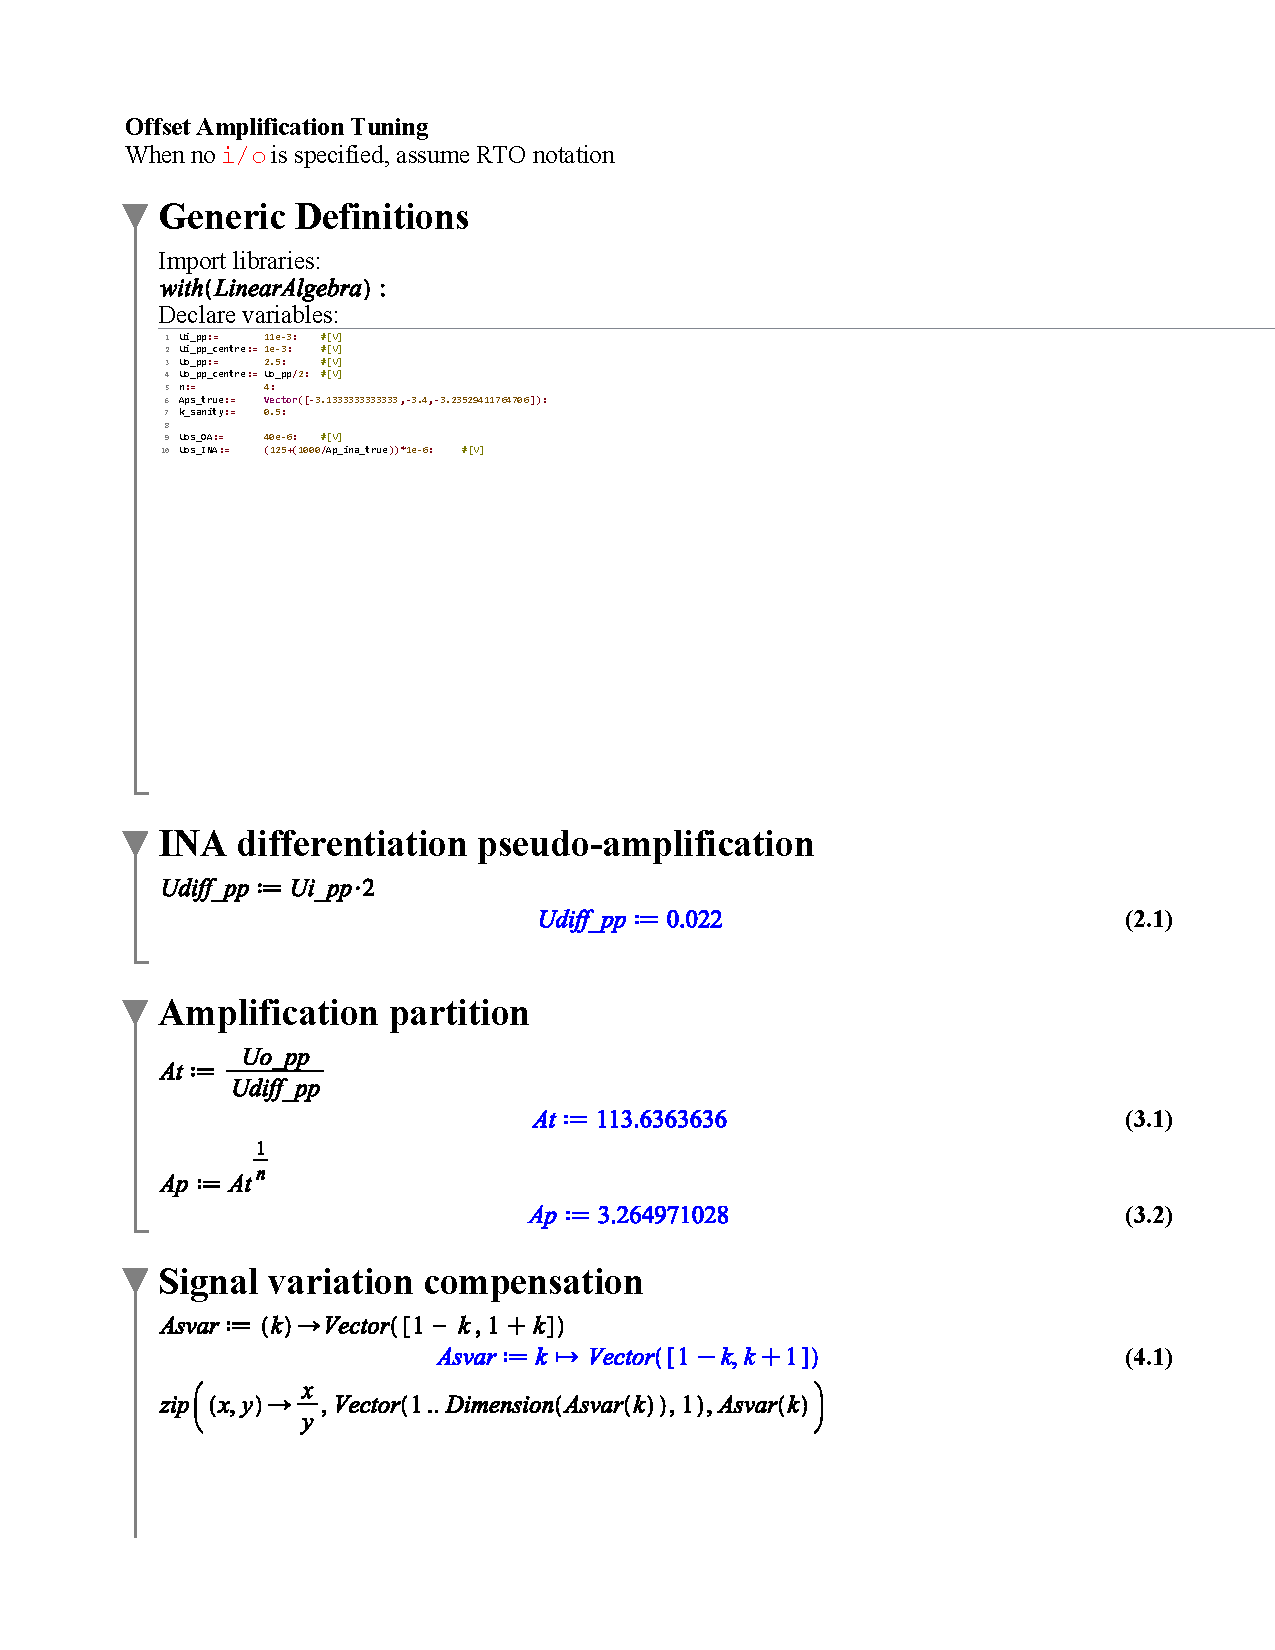
\includepdf[pages=-]{media/maple/offset_amplification_tuning.pdf}
    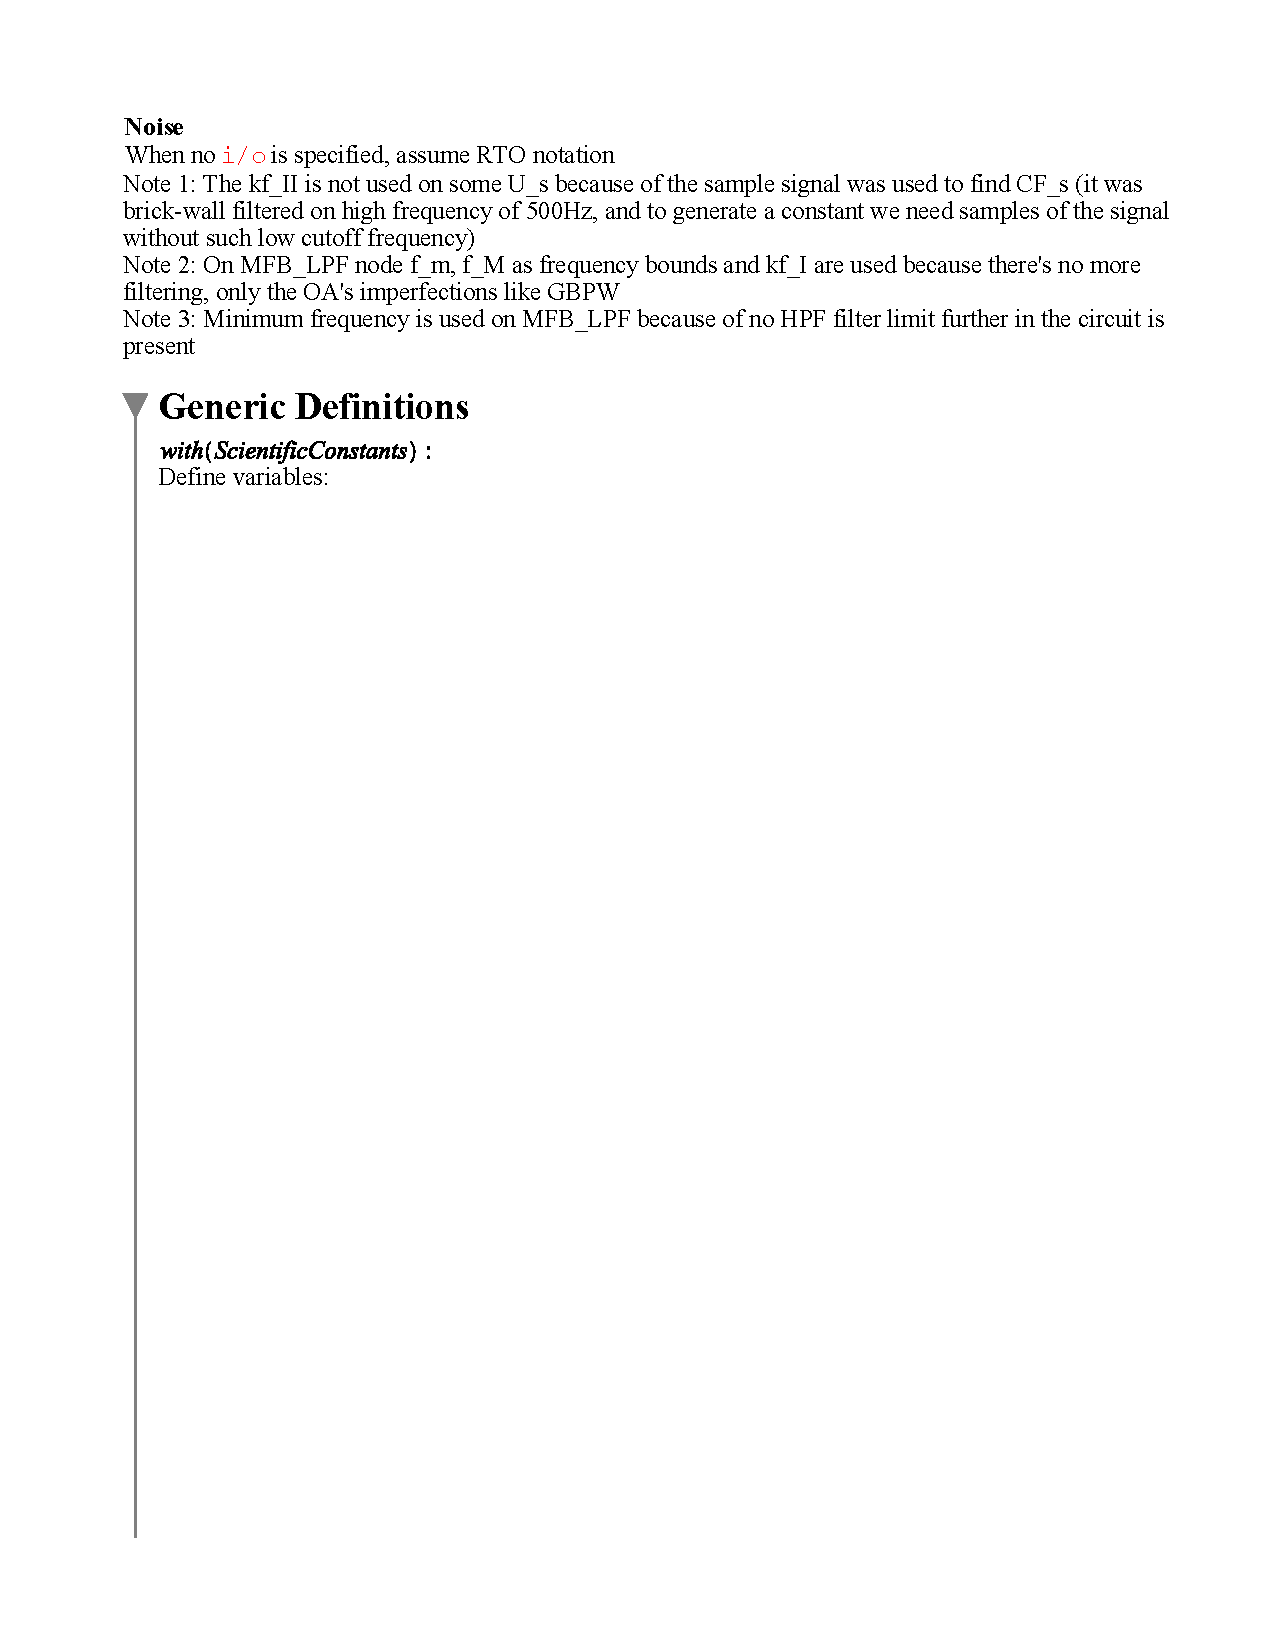
\includepdf[pages=-]{media/maple/noise.pdf}
    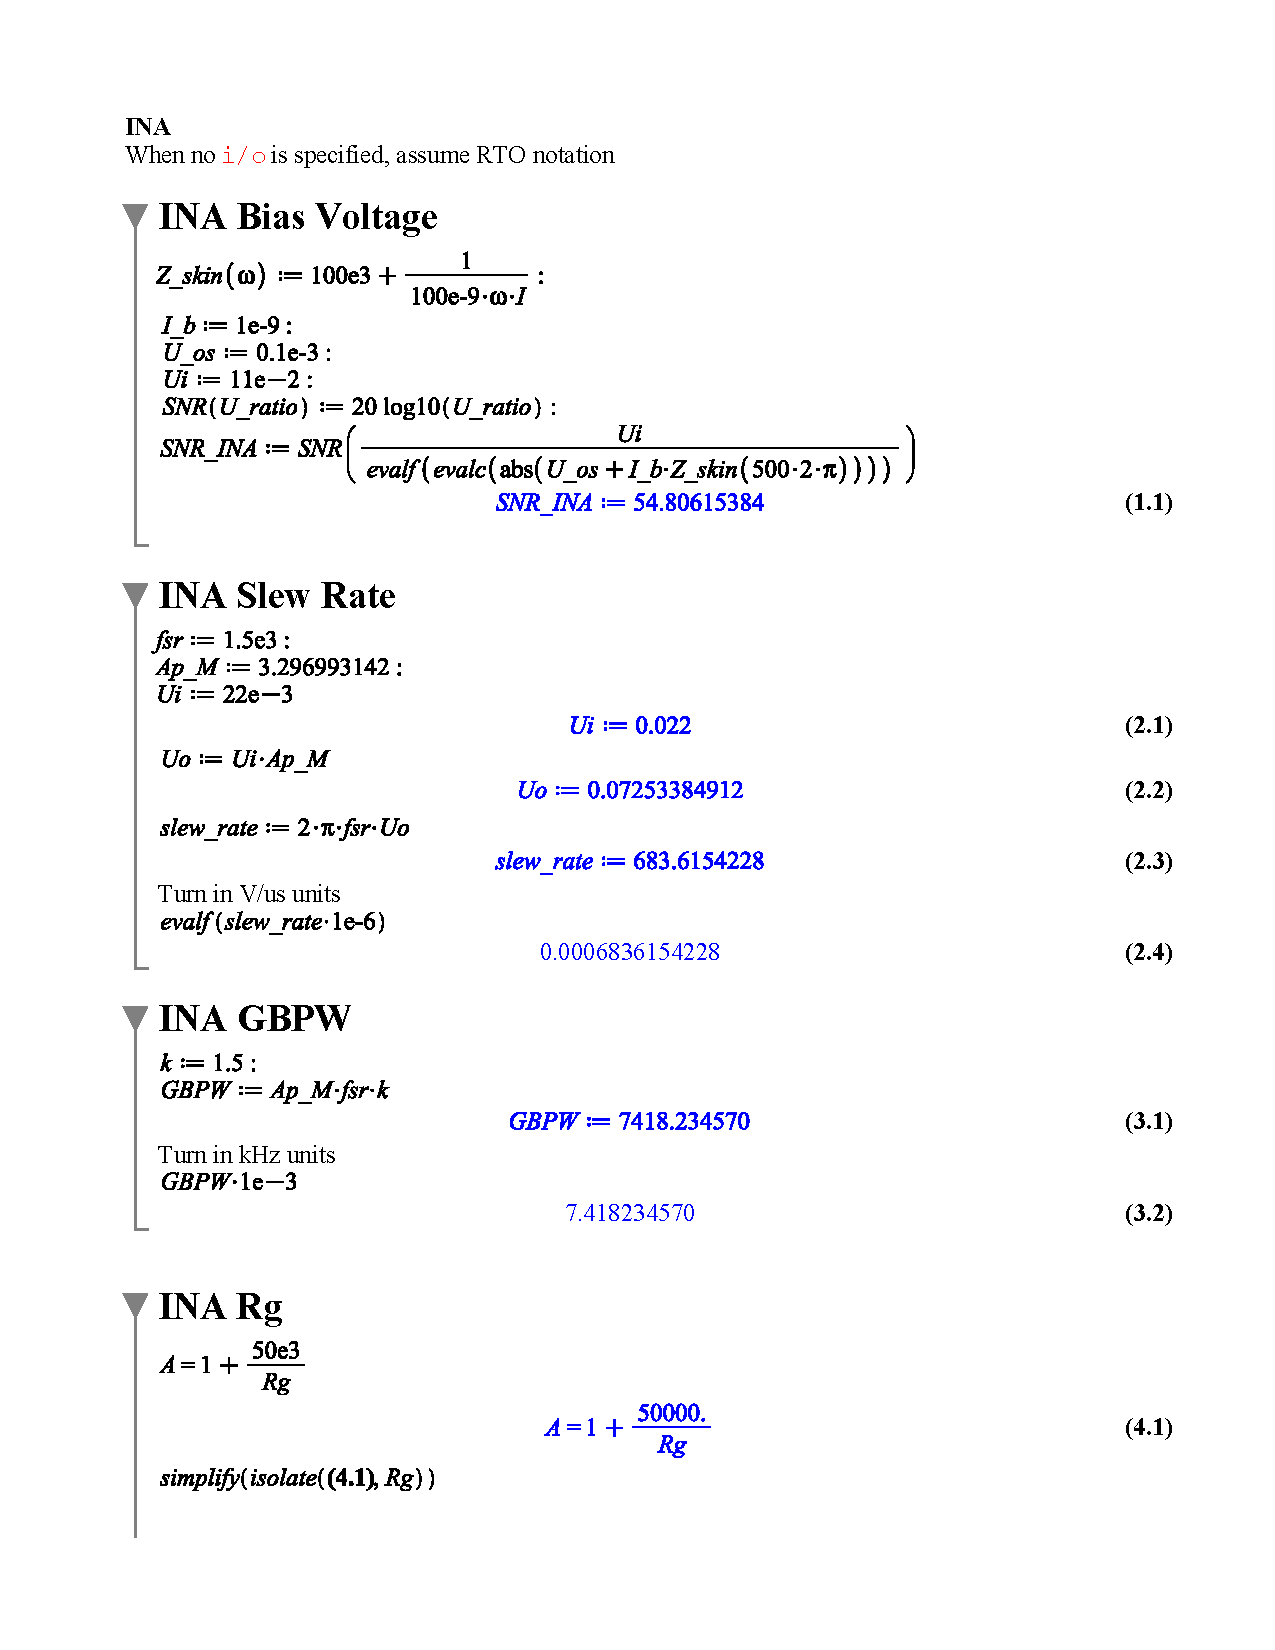
\includepdf[pages=-]{media/maple/INA.pdf}
    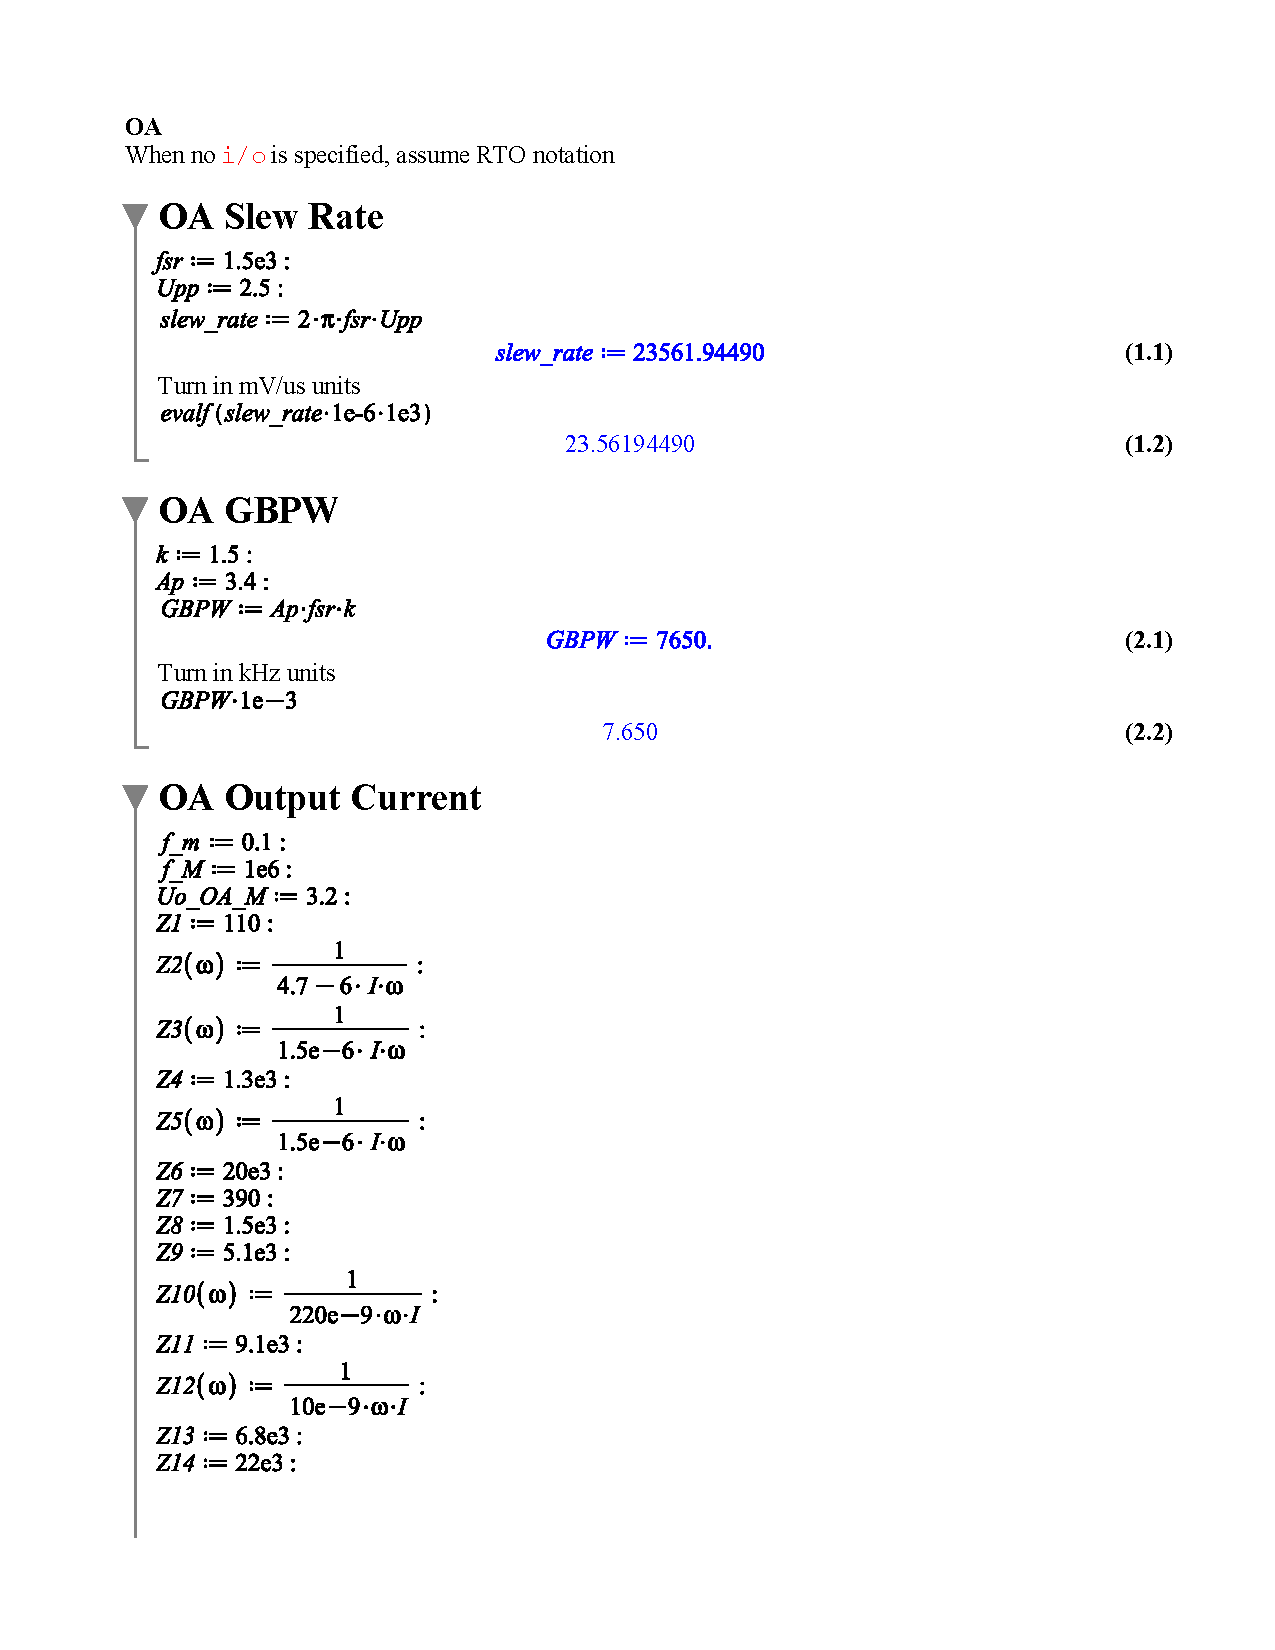
\includepdf[pages=-]{media/maple/OA.pdf}
    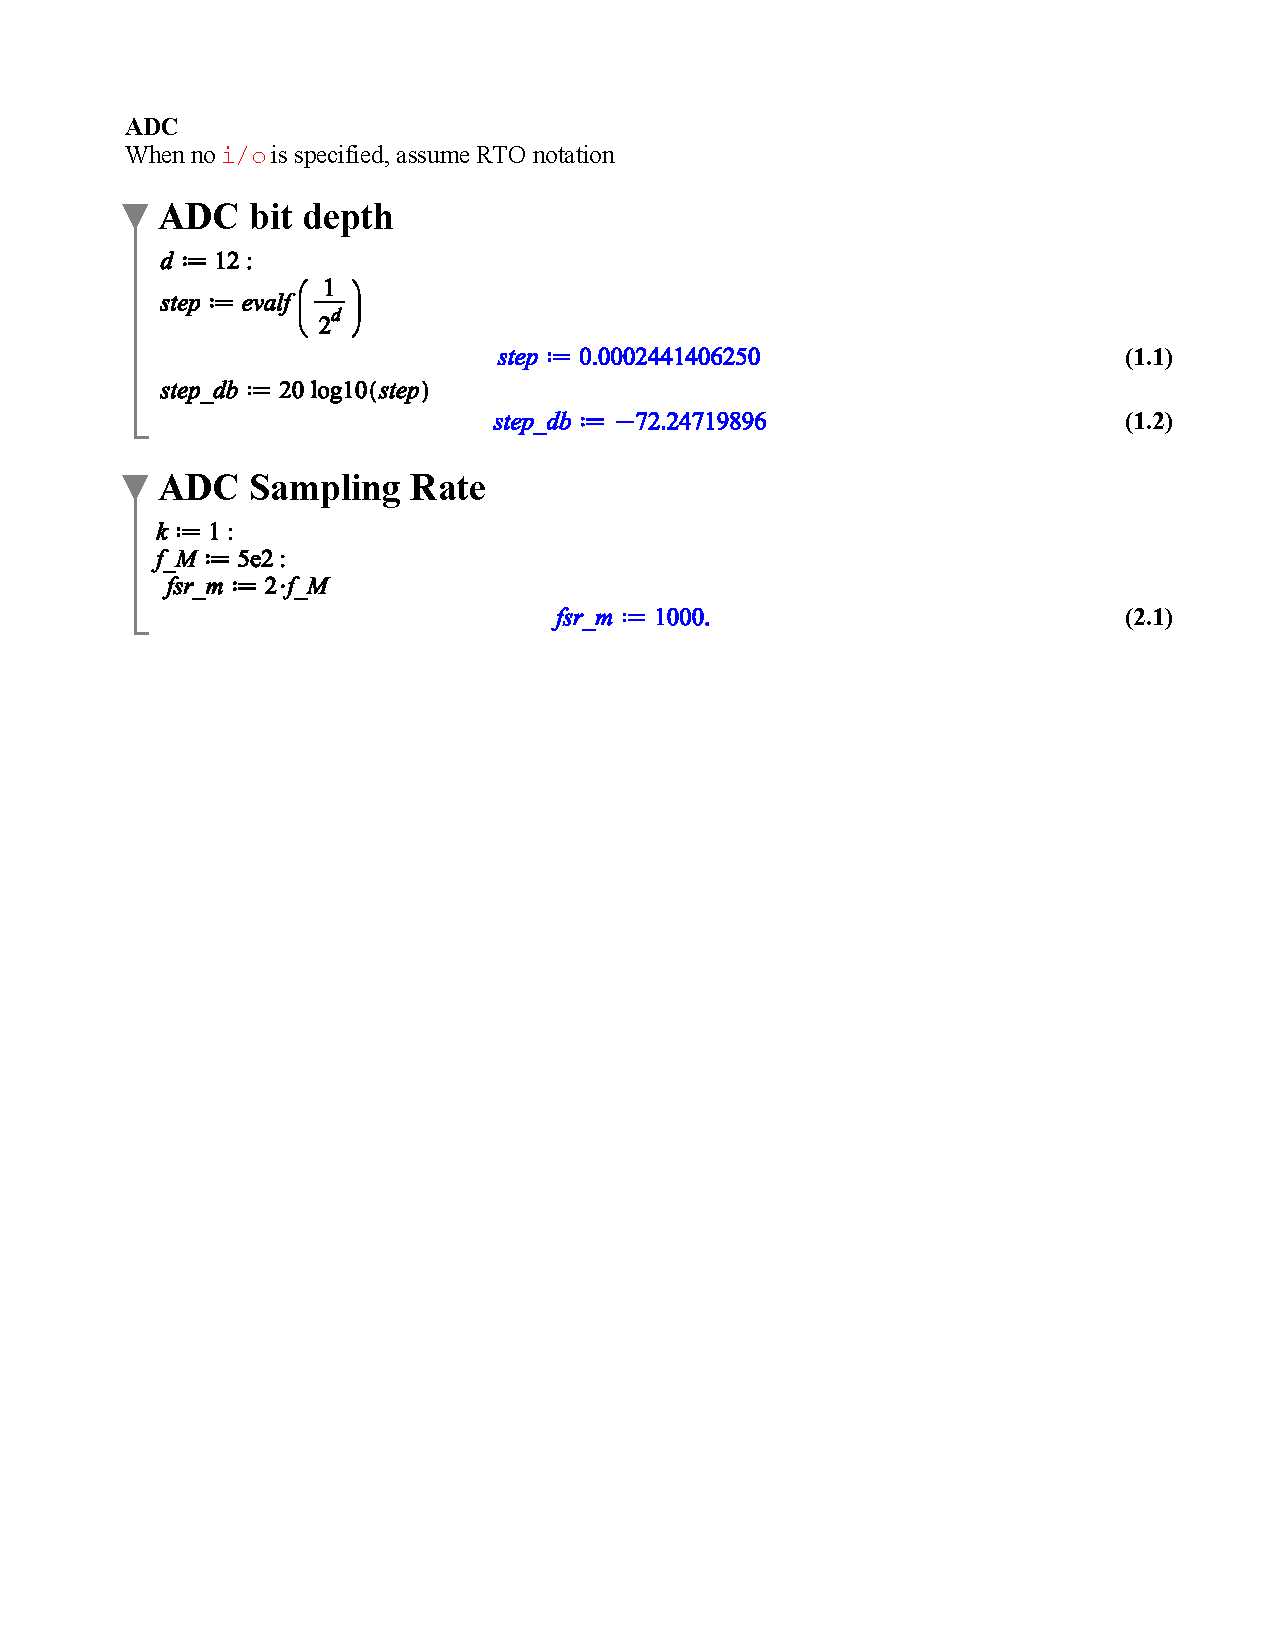
\includepdf[pages=-]{media/maple/ADC.pdf}

    \printbibheading
    \printbibliography[keyword=major, heading=subbibliography, title={Key Sources}]
    \printbibliography[keyword=minor, heading=subbibliography, title={Secondary Sources}]
    \printbibliography[keyword=data, heading=subbibliography, title={Data Sources}]
    \printbibliography[keyword=image, heading=subbibliography, title={Image Sources}]
    \printbibliography[keyword=datasheet, heading=subbibliography, title={Datasheet Sources}]
    \printbibliography[keyword=software, heading=subbibliography, title={Software Sources}]
    % TRANSLATOR NOTE: "Sorgenti Componenti" and "Sorgenti Software" were not in the given mapping; translated as "Component Sources" / "Software Sources".
    \printbibliography[keyword=web, heading=subbibliography, title={Component Sources}]
\end{document}
